% Options for packages loaded elsewhere
\PassOptionsToPackage{unicode}{hyperref}
\PassOptionsToPackage{hyphens}{url}
\PassOptionsToPackage{dvipsnames,svgnames,x11names}{xcolor}
%
\documentclass[
  letterpaper,
  DIV=11,
  numbers=noendperiod]{scrreprt}

\usepackage{amsmath,amssymb}
\usepackage{iftex}
\ifPDFTeX
  \usepackage[T1]{fontenc}
  \usepackage[utf8]{inputenc}
  \usepackage{textcomp} % provide euro and other symbols
\else % if luatex or xetex
  \usepackage{unicode-math}
  \defaultfontfeatures{Scale=MatchLowercase}
  \defaultfontfeatures[\rmfamily]{Ligatures=TeX,Scale=1}
\fi
\usepackage{lmodern}
\ifPDFTeX\else  
    % xetex/luatex font selection
\fi
% Use upquote if available, for straight quotes in verbatim environments
\IfFileExists{upquote.sty}{\usepackage{upquote}}{}
\IfFileExists{microtype.sty}{% use microtype if available
  \usepackage[]{microtype}
  \UseMicrotypeSet[protrusion]{basicmath} % disable protrusion for tt fonts
}{}
\makeatletter
\@ifundefined{KOMAClassName}{% if non-KOMA class
  \IfFileExists{parskip.sty}{%
    \usepackage{parskip}
  }{% else
    \setlength{\parindent}{0pt}
    \setlength{\parskip}{6pt plus 2pt minus 1pt}}
}{% if KOMA class
  \KOMAoptions{parskip=half}}
\makeatother
\usepackage{xcolor}
\setlength{\emergencystretch}{3em} % prevent overfull lines
\setcounter{secnumdepth}{3}
% Make \paragraph and \subparagraph free-standing
\ifx\paragraph\undefined\else
  \let\oldparagraph\paragraph
  \renewcommand{\paragraph}[1]{\oldparagraph{#1}\mbox{}}
\fi
\ifx\subparagraph\undefined\else
  \let\oldsubparagraph\subparagraph
  \renewcommand{\subparagraph}[1]{\oldsubparagraph{#1}\mbox{}}
\fi

\usepackage{color}
\usepackage{fancyvrb}
\newcommand{\VerbBar}{|}
\newcommand{\VERB}{\Verb[commandchars=\\\{\}]}
\DefineVerbatimEnvironment{Highlighting}{Verbatim}{commandchars=\\\{\}}
% Add ',fontsize=\small' for more characters per line
\usepackage{framed}
\definecolor{shadecolor}{RGB}{241,243,245}
\newenvironment{Shaded}{\begin{snugshade}}{\end{snugshade}}
\newcommand{\AlertTok}[1]{\textcolor[rgb]{0.68,0.00,0.00}{#1}}
\newcommand{\AnnotationTok}[1]{\textcolor[rgb]{0.37,0.37,0.37}{#1}}
\newcommand{\AttributeTok}[1]{\textcolor[rgb]{0.40,0.45,0.13}{#1}}
\newcommand{\BaseNTok}[1]{\textcolor[rgb]{0.68,0.00,0.00}{#1}}
\newcommand{\BuiltInTok}[1]{\textcolor[rgb]{0.00,0.23,0.31}{#1}}
\newcommand{\CharTok}[1]{\textcolor[rgb]{0.13,0.47,0.30}{#1}}
\newcommand{\CommentTok}[1]{\textcolor[rgb]{0.37,0.37,0.37}{#1}}
\newcommand{\CommentVarTok}[1]{\textcolor[rgb]{0.37,0.37,0.37}{\textit{#1}}}
\newcommand{\ConstantTok}[1]{\textcolor[rgb]{0.56,0.35,0.01}{#1}}
\newcommand{\ControlFlowTok}[1]{\textcolor[rgb]{0.00,0.23,0.31}{#1}}
\newcommand{\DataTypeTok}[1]{\textcolor[rgb]{0.68,0.00,0.00}{#1}}
\newcommand{\DecValTok}[1]{\textcolor[rgb]{0.68,0.00,0.00}{#1}}
\newcommand{\DocumentationTok}[1]{\textcolor[rgb]{0.37,0.37,0.37}{\textit{#1}}}
\newcommand{\ErrorTok}[1]{\textcolor[rgb]{0.68,0.00,0.00}{#1}}
\newcommand{\ExtensionTok}[1]{\textcolor[rgb]{0.00,0.23,0.31}{#1}}
\newcommand{\FloatTok}[1]{\textcolor[rgb]{0.68,0.00,0.00}{#1}}
\newcommand{\FunctionTok}[1]{\textcolor[rgb]{0.28,0.35,0.67}{#1}}
\newcommand{\ImportTok}[1]{\textcolor[rgb]{0.00,0.46,0.62}{#1}}
\newcommand{\InformationTok}[1]{\textcolor[rgb]{0.37,0.37,0.37}{#1}}
\newcommand{\KeywordTok}[1]{\textcolor[rgb]{0.00,0.23,0.31}{#1}}
\newcommand{\NormalTok}[1]{\textcolor[rgb]{0.00,0.23,0.31}{#1}}
\newcommand{\OperatorTok}[1]{\textcolor[rgb]{0.37,0.37,0.37}{#1}}
\newcommand{\OtherTok}[1]{\textcolor[rgb]{0.00,0.23,0.31}{#1}}
\newcommand{\PreprocessorTok}[1]{\textcolor[rgb]{0.68,0.00,0.00}{#1}}
\newcommand{\RegionMarkerTok}[1]{\textcolor[rgb]{0.00,0.23,0.31}{#1}}
\newcommand{\SpecialCharTok}[1]{\textcolor[rgb]{0.37,0.37,0.37}{#1}}
\newcommand{\SpecialStringTok}[1]{\textcolor[rgb]{0.13,0.47,0.30}{#1}}
\newcommand{\StringTok}[1]{\textcolor[rgb]{0.13,0.47,0.30}{#1}}
\newcommand{\VariableTok}[1]{\textcolor[rgb]{0.07,0.07,0.07}{#1}}
\newcommand{\VerbatimStringTok}[1]{\textcolor[rgb]{0.13,0.47,0.30}{#1}}
\newcommand{\WarningTok}[1]{\textcolor[rgb]{0.37,0.37,0.37}{\textit{#1}}}

\providecommand{\tightlist}{%
  \setlength{\itemsep}{0pt}\setlength{\parskip}{0pt}}\usepackage{longtable,booktabs,array}
\usepackage{calc} % for calculating minipage widths
% Correct order of tables after \paragraph or \subparagraph
\usepackage{etoolbox}
\makeatletter
\patchcmd\longtable{\par}{\if@noskipsec\mbox{}\fi\par}{}{}
\makeatother
% Allow footnotes in longtable head/foot
\IfFileExists{footnotehyper.sty}{\usepackage{footnotehyper}}{\usepackage{footnote}}
\makesavenoteenv{longtable}
\usepackage{graphicx}
\makeatletter
\def\maxwidth{\ifdim\Gin@nat@width>\linewidth\linewidth\else\Gin@nat@width\fi}
\def\maxheight{\ifdim\Gin@nat@height>\textheight\textheight\else\Gin@nat@height\fi}
\makeatother
% Scale images if necessary, so that they will not overflow the page
% margins by default, and it is still possible to overwrite the defaults
% using explicit options in \includegraphics[width, height, ...]{}
\setkeys{Gin}{width=\maxwidth,height=\maxheight,keepaspectratio}
% Set default figure placement to htbp
\makeatletter
\def\fps@figure{htbp}
\makeatother

\KOMAoption{captions}{tableheading}
\makeatletter
\@ifpackageloaded{tcolorbox}{}{\usepackage[skins,breakable]{tcolorbox}}
\@ifpackageloaded{fontawesome5}{}{\usepackage{fontawesome5}}
\definecolor{quarto-callout-color}{HTML}{909090}
\definecolor{quarto-callout-note-color}{HTML}{0758E5}
\definecolor{quarto-callout-important-color}{HTML}{CC1914}
\definecolor{quarto-callout-warning-color}{HTML}{EB9113}
\definecolor{quarto-callout-tip-color}{HTML}{00A047}
\definecolor{quarto-callout-caution-color}{HTML}{FC5300}
\definecolor{quarto-callout-color-frame}{HTML}{acacac}
\definecolor{quarto-callout-note-color-frame}{HTML}{4582ec}
\definecolor{quarto-callout-important-color-frame}{HTML}{d9534f}
\definecolor{quarto-callout-warning-color-frame}{HTML}{f0ad4e}
\definecolor{quarto-callout-tip-color-frame}{HTML}{02b875}
\definecolor{quarto-callout-caution-color-frame}{HTML}{fd7e14}
\makeatother
\makeatletter
\makeatother
\makeatletter
\@ifpackageloaded{bookmark}{}{\usepackage{bookmark}}
\makeatother
\makeatletter
\@ifpackageloaded{caption}{}{\usepackage{caption}}
\AtBeginDocument{%
\ifdefined\contentsname
  \renewcommand*\contentsname{Table of contents}
\else
  \newcommand\contentsname{Table of contents}
\fi
\ifdefined\listfigurename
  \renewcommand*\listfigurename{List of Figures}
\else
  \newcommand\listfigurename{List of Figures}
\fi
\ifdefined\listtablename
  \renewcommand*\listtablename{List of Tables}
\else
  \newcommand\listtablename{List of Tables}
\fi
\ifdefined\figurename
  \renewcommand*\figurename{Figure}
\else
  \newcommand\figurename{Figure}
\fi
\ifdefined\tablename
  \renewcommand*\tablename{Table}
\else
  \newcommand\tablename{Table}
\fi
}
\@ifpackageloaded{float}{}{\usepackage{float}}
\floatstyle{ruled}
\@ifundefined{c@chapter}{\newfloat{codelisting}{h}{lop}}{\newfloat{codelisting}{h}{lop}[chapter]}
\floatname{codelisting}{Listing}
\newcommand*\listoflistings{\listof{codelisting}{List of Listings}}
\makeatother
\makeatletter
\@ifpackageloaded{caption}{}{\usepackage{caption}}
\@ifpackageloaded{subcaption}{}{\usepackage{subcaption}}
\makeatother
\makeatletter
\@ifpackageloaded{tcolorbox}{}{\usepackage[skins,breakable]{tcolorbox}}
\makeatother
\makeatletter
\@ifundefined{shadecolor}{\definecolor{shadecolor}{rgb}{.97, .97, .97}}
\makeatother
\makeatletter
\makeatother
\makeatletter
\makeatother
\ifLuaTeX
  \usepackage{selnolig}  % disable illegal ligatures
\fi
\IfFileExists{bookmark.sty}{\usepackage{bookmark}}{\usepackage{hyperref}}
\IfFileExists{xurl.sty}{\usepackage{xurl}}{} % add URL line breaks if available
\urlstyle{same} % disable monospaced font for URLs
\hypersetup{
  pdftitle={STA 2450 Computing for Math \& Stat},
  colorlinks=true,
  linkcolor={blue},
  filecolor={Maroon},
  citecolor={Blue},
  urlcolor={Blue},
  pdfcreator={LaTeX via pandoc}}

\title{STA 2450 Computing for Math \& Stat}
\author{}
\date{}

\begin{document}
\maketitle
\ifdefined\Shaded\renewenvironment{Shaded}{\begin{tcolorbox}[boxrule=0pt, interior hidden, enhanced, frame hidden, sharp corners, borderline west={3pt}{0pt}{shadecolor}, breakable]}{\end{tcolorbox}}\fi

\renewcommand*\contentsname{Table of contents}
{
\hypersetup{linkcolor=}
\setcounter{tocdepth}{2}
\tableofcontents
}
\bookmarksetup{startatroot}

\hypertarget{introduction}{%
\chapter*{Introduction}\label{introduction}}
\addcontentsline{toc}{chapter}{Introduction}

\markboth{Introduction}{Introduction}

These are the lecture notes for STA 2450 - Computing for Math \& Stat.

\textbf{Prerequisites:} None

\hypertarget{course-description}{%
\subsubsection*{Course Description:}\label{course-description}}
\addcontentsline{toc}{subsubsection}{Course Description:}

Computer programming for mathematical scientists with emphasis on
designing algorithms, problem solving, and coding practices. Topics
include development of programs from specifications; appropriate use of
data types; functions; modular program organization; documentation and
style; and version control and collaborative programming.

\bookmarksetup{startatroot}

\hypertarget{an-intro-to-computing}{%
\chapter{An Intro to Computing}\label{an-intro-to-computing}}

In the early 9th century AD, the Persian scholar Muhammad ibn Musa
al-Khwarizmi authored a book that significantly influenced the
development of European mathematics. Titled ``Al-Kitāb al-mukhtaṣar fī
ḥisāb al-jabr wa'l-muqābala'' (``The Compendious Book on Calculation by
Completion and Balancing''), Al-Khwarizmi introduced a collection of
rules for solving linear and quadratic equations based on intuitive
geometric arguments to the Western world. This work was translated into
Latin in the 12th century, leading to the term algebra (the Latin title
of the book is ``Liber Algebræ et Almucabola''). Although algebra had
earlier roots in Greece, it was Al-Khwarizmi's book that made it
accessible to European mathematicians, and it also laid the foundations
for algorithms.

An algorithm is a finite, well-defined sequence of computational
instructions or steps designed to perform a specific task or solve a
particular problem. Each step in an algorithm is precise and
unambiguous, and the algorithm is expected to produce a desired output
within a finite amount of time. Algorithms are fundamental to computer
science and mathematics, providing a systematic method for
problem-solving and decision-making.

Let's consider making a pot of coffee as an example of an algorithm.
Here's a simple, step-by-step process:

\begin{enumerate}
\def\labelenumi{\arabic{enumi}.}
\tightlist
\item
  \textbf{Fill the Coffee Maker with Water}: Measure and pour the
  required amount of water into the coffee maker's reservoir.
\item
  \textbf{Place the Coffee Filter}: Open the filter compartment and
  place a coffee filter inside.
\item
  \textbf{Add Coffee Grounds}: Measure the appropriate amount of coffee
  grounds and pour them into the filter.
\item
  \textbf{Close the Filter Compartment}: Securely close the filter
  compartment.
\item
  \textbf{Turn On the Coffee Maker}: Press the power button to start the
  brewing process.
\item
  \textbf{Wait for the Coffee to Brew}: Allow the coffee maker to
  complete its brewing cycle.
\item
  \textbf{Serve the Coffee}: Once the brewing is finished, pour the
  freshly brewed coffee into a cup and enjoy.
\end{enumerate}

Each step in this process must be followed in the correct order to
successfully make a pot of coffee, illustrating the fundamental nature
of algorithms in organizing and executing tasks.

Algorithms are like recipes for computing. They provide instructions on
how to solve problems, find answers, or move from point A to point B
using only the resources available in your computer's memory.

\hypertarget{algorithms-on-computers}{%
\section{Algorithms on Computers}\label{algorithms-on-computers}}

One way to illustrate the concept of a recipe in a mechanical process is
by designing machines specifically intended to solve certain problems.
The earliest computers were \textbf{fixed-program} computers, meaning
they were designed to solve a specific mathematical problem. Some simple
computers still use this approach. For example, a four-function
calculator can perform basic arithmetic but is not designed for word
processing or gaming. Users cannot change their programs without
replacing internal components.

The first modern computer to run a program was the Manchester Mark 1 in
1949. Unlike its predecessors, it was a \textbf{stored-program}
computer. These machines store sequences of instructions that can be
executed by an \textbf{interpreter}. This interpreter can execute any
legal set of instructions, enabling it to compute anything that can be
described using those instructions. The program and the data it
manipulates reside in memory.

Typically, a program \textbf{counter} points to a specific location in
memory, and computation starts by executing the instruction at that
point. Most often, the interpreter simply proceeds to the next
instruction in the sequence. However, in some cases, it performs a test,
and based on that test, execution may jump to another point in the
sequence of instructions.

\hypertarget{programming-languages}{%
\section{Programming Languages}\label{programming-languages}}

To use execute algorithms on a computer, we need a programming language
to describe the sequence of instructions. The British mathematician Alan
Turing devised a theoretical device in 1936 known as the Universal
Turing Machine. This hypothetical computer had unlimited memory,
represented by a tape on which one could write zeroes and ones. It also
consisted of simple instructions for moving, reading, and writing on the
tape.

The Church-Turing thesis posits that if a function is computable, a
Turing Machine can be programmed to compute it. The ``if'' in the
Church-Turing thesis is crucial because not all problems have
computational solutions.

\begin{tcolorbox}[enhanced jigsaw, coltitle=black, colback=white, bottomrule=.15mm, arc=.35mm, titlerule=0mm, opacitybacktitle=0.6, toptitle=1mm, left=2mm, toprule=.15mm, opacityback=0, bottomtitle=1mm, title=\textcolor{quarto-callout-note-color}{\faInfo}\hspace{0.5em}{Note}, rightrule=.15mm, colframe=quarto-callout-note-color-frame, breakable, colbacktitle=quarto-callout-note-color!10!white, leftrule=.75mm]

A function or problem is considered \textbf{computable} if there exists
a finite sequence of well-defined steps, an algorithm, that can be
implemented by a computational model (such as a Turing Machine) to
produce the correct output for any valid input within a finite amount of
time. In other words, a problem is computable if there is a systematic
method to solve it using an algorithm.

\end{tcolorbox}

The Church-Turing thesis leads directly to the concept of Turing
completeness. A programming language is said to be \textbf{Turing
complete} if it can simulate a universal Turing Machine. All modern
programming languages are Turing complete, meaning that anything that
can be programmed in one language (e.g., Python) can also be programmed
in another language (e.g., Java). While certain tasks may be easier to
program in specific languages, all languages are fundamentally equal in
terms of computational power.

\hypertarget{types-of-programming-languages}{%
\section{Types of Programming
Languages}\label{types-of-programming-languages}}

\hypertarget{low-level-vs.-high-level-languages}{%
\subsection{Low-Level vs.~High-Level
Languages}\label{low-level-vs.-high-level-languages}}

\textbf{Low-level} languages are closer to machine language, providing
little to no abstraction from a computer's hardware. They allow direct
control over the hardware and memory, making them highly efficient but
also more complex to write and understand. Examples of low-level
languages include Assembly language and machine code.

Low-level languages operate with minimal abstraction which results in
high-performance programs that execute faster and are more efficient in
resource usage. However, this comes with the trade-off of complex and
less intuitive code, requiring a deep understanding of computer
architecture. Additionally, low-level programs are often
platform-specific, meaning they are tailored to a particular type of
processor or computer architecture.

\hypertarget{example-assembly-language}{%
\paragraph{Example: Assembly Language}\label{example-assembly-language}}

\begin{Shaded}
\begin{Highlighting}[]
\NormalTok{MOV AX, 1   ; Move the value 1 into the AX register}
\NormalTok{ADD AX, 2   ; Add the value 2 to the AX register}
\NormalTok{MOV BX, AX  ; Move the result from AX to BX}
\end{Highlighting}
\end{Shaded}

\textbf{High-level} languages abstract away the details of computer
hardware, allowing programmers to focus on the logic of the problem
rather than the intricacies of the machine. They feature more intuitive
syntax and semantics, making them easier to learn and use. Programs
written in high-level languages are generally portable across different
platforms with minimal modification. These languages also come with
extensive libraries and frameworks that simplify complex tasks such as
GUI development, web programming, and data manipulation. Although this
abstraction can result in slower execution compared to low-level
languages, the trade-off is often worth it for the ease of development
and maintenance.

\hypertarget{example-print-a-greeting-to-the-screen-in-python}{%
\paragraph{Example: Print a greeting to the screen in
Python}\label{example-print-a-greeting-to-the-screen-in-python}}

\begin{Shaded}
\begin{Highlighting}[]
\BuiltInTok{print}\NormalTok{(}\StringTok{"Hello, World!"}\NormalTok{)  }
\end{Highlighting}
\end{Shaded}

Low-level languages offer greater control over hardware and performance
optimization, whereas high-level languages prioritize ease of use and
development speed. This means that while low-level languages generally
result in faster and more efficient programs, they come at the cost of
greater complexity. In contrast, high-level languages, although
potentially slower, provide significant productivity benefits. Their
readability and maintainability make them suitable for large-scale
applications and collaborative projects. Additionally, high-level
languages reduce development time due to their simplicity and the
availability of powerful libraries and frameworks.

Understanding the trade-offs between low-level and high-level languages
is crucial for selecting the right tool for a given task. For most
applications, high-level languages provide sufficient performance while
dramatically simplifying development. However, for performance-critical
applications, such as operating system kernels or embedded systems,
low-level languages remain indispensable.

\hypertarget{general-purpose-vs.-domain-specific-languages}{%
\subsection{General-Purpose vs.~Domain-Specific
Languages}\label{general-purpose-vs.-domain-specific-languages}}

\textbf{General-purpose} programming languages are highly versatile,
allowing them to be used for a wide array of programming tasks,
including web development, data analysis, game development, and more.
They come with extensive standard libraries and frameworks that support
diverse functionalities, making it easier to implement complex features.
Programs written in these languages are often portable across different
operating systems and platforms. Additionally, these languages usually
have large communities, extensive documentation, and abundant resources
for learning and troubleshooting. Examples of well-known general-purpose
programming languages include Python, Java, C++, and JavaScript.

\textbf{Domain-specific} Domain-specific languages (DSLs) are designed
to handle specific types of tasks, offering features and abstractions
directly relevant to their domain. They often allow for more concise and
efficient coding within their domain, reducing the complexity and effort
required to develop certain applications. However, their functionality
is typically narrow, focusing on particular problem areas and lacking
the versatility of general-purpose languages. Examples of well-known
domain-specific languages include SQL, HTML, and MATLAB.

General-purpose languages are suitable for a wide variety of
applications, providing greater flexibility and usability across many
contexts. In contrast, domain-specific languages are specialized for
particular tasks, making them more efficient and easier to use within
their specific domains. While general-purpose languages often require
learning a broader set of concepts and syntax, domain-specific languages
might have a steeper but narrower learning curve focused on their
particular use case.

\hypertarget{interpreted-vs.-compiled-languages}{%
\subsection{Interpreted vs.~Compiled
Languages}\label{interpreted-vs.-compiled-languages}}

\textbf{Interpreted} languages execute code directly through an
interpreter, which translates high-level instructions into machine code
line by line. This immediate execution provides several advantages, such
as ease of debugging, as interpreted languages often generate more
informative error messages, making it simpler to identify and correct
issues by pointing to the exact line where an error occurred.
Additionally, interpreted languages offer platform independence,
allowing the same source code to run on any platform with a compatible
interpreter, enhancing portability. However, interpreted programs
generally run slower than compiled programs because the translation
occurs at runtime. Well-known interpreted languages include Python,
JavaScript, Ruby, and PHP.

\textbf{Compiled} languages require the source code to be translated
into machine code by a compiler before execution, producing an
executable file. This pre-execution compilation results in faster
execution, as the translation is completed beforehand, allowing the
executable file to be directly executed by the hardware. Compilers also
perform extensive checks during compilation, catching many types of
errors before the program runs. However, compiled executables are
specific to the target platform's architecture, making them less
portable unless recompiled for different platforms. Well-known compiled
languages include C, C++, Rust, and Go.

\hypertarget{example-of-c-code}{%
\paragraph{Example of C Code:}\label{example-of-c-code}}

\begin{Shaded}
\begin{Highlighting}[]
\PreprocessorTok{\#include }\ImportTok{\textless{}stdio.h\textgreater{}}

\DataTypeTok{int}\NormalTok{ main}\OperatorTok{()} \OperatorTok{\{}
\NormalTok{    printf}\OperatorTok{(}\StringTok{"Hello, World!}\SpecialCharTok{\textbackslash{}n}\StringTok{"}\OperatorTok{);}
    \ControlFlowTok{return} \DecValTok{0}\OperatorTok{;}
\OperatorTok{\}}
\end{Highlighting}
\end{Shaded}

This C code must be compiled into an executable file before it can be
run.

Compiled languages generally produce faster-running programs since the
code is translated into machine language ahead of time, whereas
interpreted languages tend to be slower due to on-the-fly translation.
However, interpreted languages offer a quicker development cycle,
allowing code to be written and tested immediately without a separate
compilation step, which is advantageous for rapid prototyping and
iterative development. Interpreted languages also boast better
portability, as the same code can run on any platform with the
appropriate interpreter, while compiled languages require recompilation
for different platforms, adding complexity.

Debugging is typically easier with interpreted languages because they
provide more immediate and informative error feedback, pointing directly
to issues in the source code. Although compiled languages catch many
errors at compile time, their runtime error messages can be less
detailed. Additionally, interpreted languages can support more dynamic
programming features, such as dynamic typing and runtime evaluation of
code, which can be more challenging to implement efficiently in compiled
languages.

\hypertarget{intro-to-python}{%
\section{Intro to Python}\label{intro-to-python}}

In this course, we will be using Python. Python is a general-purpose
programming language that can be used to build almost any kind of
program that does not require direct access to the computer's hardware.
However, Python is not optimal for programs with high reliability
constraints or those that are built and maintained by many people over a
long period.

Python has several advantages over many other languages. It is
relatively simple and easy to learn. Because Python is designed to be
interpreted, it provides runtime feedback that is especially helpful for
novice programmers.

Python was first developed by Guido van Rossum in 1990. It went largely
unnoticed during its first decade but gained popularity around 2000 with
the release of Python 2.0. Python 3.0, released at the end of 2008,
cleaned up many inconsistencies in Python 2's design. While Python 3.0
is not backward-compatible with earlier versions, most important public
domain libraries have been ported over, eliminating the need to use
outdated software.

\bookmarksetup{startatroot}

\hypertarget{installing-python-and-setting-up-your-ide}{%
\chapter{Installing Python and Setting Up Your
IDE}\label{installing-python-and-setting-up-your-ide}}

\hypertarget{installing-python}{%
\section{Installing Python}\label{installing-python}}

To start programming in Python, you'll first need to install Python on
your computer. Follow the instructions below based on your operating
system:

\textbf{Windows:}

\begin{enumerate}
\def\labelenumi{\arabic{enumi}.}
\tightlist
\item
  Go to the official Python website:
  \href{https://www.python.org/}{python.org}.
\item
  Click on the ``Downloads'' tab.
\item
  Download the latest version of Python (ensure it's a stable release).
\item
  Run the installer and make sure to check the box that says ``Add
  Python to PATH''.
\item
  Follow the installation prompts.
\end{enumerate}

\textbf{macOS:}

\begin{enumerate}
\def\labelenumi{\arabic{enumi}.}
\item
  Open Terminal.
\item
  Use Homebrew to install Python (if you don't have Homebrew, you can
  install it from \href{https://brew.sh/}{brew.sh}):

\begin{Shaded}
\begin{Highlighting}[]
\NormalTok{/bin/bash {-}c "$(curl {-}fsSL https://raw.githubusercontent.com/Homebrew/install/HEAD/install.sh)"}
\end{Highlighting}
\end{Shaded}
\item
  Install Python:

\begin{Shaded}
\begin{Highlighting}[]
\NormalTok{brew install python}
\end{Highlighting}
\end{Shaded}
\end{enumerate}

\textbf{Linux:}

\begin{enumerate}
\def\labelenumi{\arabic{enumi}.}
\item
  Open Terminal.
\item
  Use your package manager to install Python. For Debian-based systems
  like Ubuntu:

\begin{Shaded}
\begin{Highlighting}[]
\NormalTok{sudo apt update}
\NormalTok{sudo apt install python3}
\end{Highlighting}
\end{Shaded}

  For Red Hat-based systems like Fedora:

\begin{Shaded}
\begin{Highlighting}[]
\NormalTok{sudo dnf install python3}
\end{Highlighting}
\end{Shaded}
\end{enumerate}

To verify the installation, open your terminal or command prompt and
type:

\begin{Shaded}
\begin{Highlighting}[]
\NormalTok{python {-}{-}version}
\end{Highlighting}
\end{Shaded}

You should see the installed Python version displayed.

\hypertarget{understanding-integrated-development-environments-ides}{%
\section{Understanding Integrated Development Environments
(IDEs)}\label{understanding-integrated-development-environments-ides}}

\hypertarget{what-is-an-ide}{%
\subsubsection{What is an IDE?}\label{what-is-an-ide}}

An Integrated Development Environment (IDE) is a software application
that provides comprehensive facilities to programmers for software
development. An IDE typically includes:

\begin{enumerate}
\def\labelenumi{\arabic{enumi}.}
\tightlist
\item
  \textbf{Source Code Editor}: A text editor that supports code writing
  with features like syntax highlighting, auto-completion, and error
  detection.
\item
  \textbf{Build Automation Tools}: Tools that automate tasks like
  compiling code, packaging files, and running tests.
\item
  \textbf{Debugger}: A tool that helps you test and debug your code by
  allowing you to step through your code, set breakpoints, and inspect
  variables.
\end{enumerate}

IDEs are designed to make the process of coding easier and more
efficient by combining all the tools you need into a single application.

\hypertarget{benefits-of-using-an-ide}{%
\subsubsection{Benefits of Using an
IDE}\label{benefits-of-using-an-ide}}

Using an IDE offers numerous benefits and features that enhance the
coding process. An IDE can significantly speed up development by
providing quick access to all necessary tools, enhancing efficiency.
Features like syntax highlighting and error detection help catch
mistakes early, reducing the amount of debugging needed, thereby
improving error reduction.

The convenience of having everything in one place makes it easier to
manage projects, especially as they grow in size and complexity.
Additionally, many IDEs include tools for version control, making it
easier to track changes and collaborate with others, thus improving code
management.

Key features of an IDE streamline the coding process further. Syntax
highlighting colors keywords, variables, and syntax, making the code
more readable and easier to debug. Auto-completion suggests code
completions as you type, helping to write code faster and avoid typos.
Code navigation allows you to quickly jump to definitions, references,
and files within your project. The integrated debugger lets you run your
code step by step, inspect variables, and identify issues.

\hypertarget{popular-python-ides}{%
\subsubsection{Popular Python IDEs}\label{popular-python-ides}}

\begin{itemize}
\tightlist
\item
  \textbf{PyCharm}: A powerful IDE specifically for Python development,
  offering advanced features and professional tools.
\item
  \textbf{RStudio}: Primarily used for R programming but also supports
  Python, providing a familiar interface for those who use both
  languages.
\item
  \textbf{Visual Studio Code}: A versatile code editor with extensive
  Python support through extensions, combining lightweight design with
  powerful features.
\end{itemize}

\hypertarget{choosing-an-ide}{%
\subsubsection{Choosing an IDE}\label{choosing-an-ide}}

Choosing the right IDE depends on your needs and preferences. Some
factors to consider include ease of use, which refers to how intuitive
and user-friendly the IDE is, and the feature set, which involves the
availability of features that match your development needs. Performance
is also crucial, particularly how well the IDE performs with larger
projects. Additionally, consider the community and support available,
including documentation, tutorials, and community support.

Whether you use PyCharm, RStudio, or another IDE, having a good
development environment can make a significant difference in your
productivity and the quality of your code. A well-chosen IDE enhances
your coding experience, making it easier to write, manage, and debug
your projects efficiently.

\hypertarget{setting-up-your-ide}{%
\section{Setting Up Your IDE}\label{setting-up-your-ide}}

\textbf{Using PyCharm:}

PyCharm, developed by JetBrains, is a popular IDE specifically designed
for Python programming. JetBrains, a software development company based
in Prague, Czech Republic, was founded in 2000 and has since become
renowned for creating intelligent, productivity-enhancing tools for
software developers. The journey of PyCharm began in 2010, when
JetBrains identified the need for a dedicated, feature-rich IDE for
Python developers. At that time, Python was gaining significant traction
due to its simplicity and versatility, and there was a growing demand
for an IDE that could cater specifically to Python's unique
requirements.

JetBrains leveraged its extensive experience in creating IDEs, such as
IntelliJ IDEA for Java, to develop PyCharm. They aimed to build an IDE
that would not only support the standard features expected by
developers, such as code completion and debugging, but also include
advanced capabilities like scientific computing support, web development
frameworks, and robust version control integration. PyCharm quickly
became popular within the Python community for its powerful features,
intuitive user interface, and the comprehensive support it provided for
various Python frameworks and libraries. Over the years, PyCharm has
continued to evolve, incorporating feedback from its user base and
keeping pace with the latest advancements in Python development.

Here's how to set up PyCharm:

\begin{enumerate}
\def\labelenumi{\arabic{enumi}.}
\tightlist
\item
  Download and Install PyCharm:

  \begin{itemize}
  \tightlist
  \item
    Go to the JetBrains website:
    \href{https://www.jetbrains.com/pycharm/download/}{jetbrains.com/pycharm/download}.
  \item
    Choose the Community edition (it's free).
  \item
    Follow the installation instructions for your operating system.
  \end{itemize}
\item
  Configuring PyCharm:

  \begin{itemize}
  \tightlist
  \item
    Open PyCharm.
  \item
    Select ``New Project''.
  \item
    Choose a location for your project.
  \item
    Ensure the Python interpreter is set correctly. If Python is not
    listed, click on ``Existing interpreter'' and locate your Python
    installation.
  \item
    Click ``Create''.
  \end{itemize}
\item
  Writing Your First Program:

  \begin{itemize}
  \item
    Right-click on your project folder in the Project pane.
  \item
    Select ``New'' \textgreater{} ``Python File''.
  \item
    Name your file (e.g., \texttt{hello\_world.py}).
  \item
    Type the following code:

\begin{Shaded}
\begin{Highlighting}[]
\BuiltInTok{print}\NormalTok{(}\StringTok{"Hello, world!"}\NormalTok{)}
\end{Highlighting}
\end{Shaded}
  \item
    Right-click on the file and select ``Run'' to execute your code.
  \end{itemize}
\end{enumerate}

\textbf{Using RStudio:}

RStudio, developed by RStudio, PBC, is a comprehensive IDE primarily
designed for the R programming language. The inception of RStudio dates
back to 2008, when its founders, including JJ Allaire, sought to create
a powerful tool to support the growing community of R users. R, a
language and environment for statistical computing and graphics, was
gaining popularity among statisticians and data scientists due to its
robust capabilities for data analysis and visualization. However, the
available development tools for R at that time were limited, and there
was a clear need for a more sophisticated and user-friendly IDE.

JJ Allaire, already an experienced software developer known for creating
the ColdFusion web development platform, aimed to fill this gap by
developing RStudio. The initial release of RStudio in 2011 was met with
enthusiasm from the R community. It offered a user-friendly interface,
integrating essential features like a source code editor, console,
workspace, and graphics viewer within a single window. This made it
significantly easier for users to write, debug, and visualize their R
code.

Over the years, RStudio has expanded its functionality to support not
only R but also other programming languages like Python, enhancing its
utility for data scientists and statisticians. The open-source nature of
RStudio and its commitment to the R community have contributed to its
widespread adoption. Today, RStudio is a central tool in data science,
used by individuals and organizations worldwide for data analysis,
research, and reporting.

Here's how to set up RStudio:

\begin{enumerate}
\def\labelenumi{\arabic{enumi}.}
\tightlist
\item
  Download and Install RStudio:

  \begin{itemize}
  \tightlist
  \item
    Go to the RStudio website:
    \href{https://rstudio.com/products/rstudio/download/}{rstudio.com}.
  \item
    Download the free version for your operating system.
  \item
    Follow the installation instructions.
  \end{itemize}
\item
  Configuring RStudio for Python:

  \begin{itemize}
  \tightlist
  \item
    Open RStudio.
  \item
    Go to ``Tools'' \textgreater{} ``Global Options''.
  \item
    Select ``Python'' from the menu on the left.
  \item
    Set the Python interpreter to your installed Python version (e.g.,
    \texttt{/usr/bin/python3} or
    \texttt{C:\textbackslash{}Python39\textbackslash{}python.exe}).
  \end{itemize}
\item
  Writing Your First Program:

  \begin{itemize}
  \item
    Go to ``File'' \textgreater{} ``New File'' \textgreater{} ``Python
    Script''.
  \item
    Type the following code:

\begin{Shaded}
\begin{Highlighting}[]
\BuiltInTok{print}\NormalTok{(}\StringTok{"Hello, world!"}\NormalTok{)}
\end{Highlighting}
\end{Shaded}
  \item
    Save the file with a \texttt{.py} extension (e.g.,
    \texttt{hello\_world.py}).
  \item
    Click the ``Run'' button to execute your code.
  \end{itemize}
\end{enumerate}

By following these instructions, you'll have Python installed and be
ready to start coding with PyCharm or RStudio as your IDE.

\hypertarget{using-google-colab}{%
\section{Using Google Colab}\label{using-google-colab}}

Google Colab is a powerful tool that allows you to write and run Python
code in a browser. It provides free access to computing resources,
including GPU and TPU options, making it ideal for learning,
experimenting, or running intensive computations without needing a
high-performance computer. Colab is built on Jupyter Notebooks, which
means you can easily share your code and outputs.

In this section, The following will be covered:

\begin{enumerate}
\def\labelenumi{\arabic{enumi}.}
\tightlist
\item
  Accessing and using Google Colab
\item
  Connecting to your Google Drive
\item
  Installing additional Python packages in Colab
\end{enumerate}

\hypertarget{accessing-google-colab}{%
\subsection{Accessing Google Colab}\label{accessing-google-colab}}

To access Google Colab, simply navigate to
\url{https://colab.research.google.com} in your browser. You can start a
new notebook by selecting \texttt{New\ Notebook} from the main
dashboard.

Alternatively, if you have a Jupyter Notebook (.ipynb) saved on your
local machine or in Google Drive, you can upload and work on it
directly.

\hypertarget{connecting-google-drive-to-colab}{%
\subsection{Connecting Google Drive to
Colab}\label{connecting-google-drive-to-colab}}

One of the most useful features of Google Colab is its ability to
connect directly to your Google Drive, allowing you to load and save
files with ease.

Here's how to connect your Google Drive to your Colab notebook:

\begin{enumerate}
\def\labelenumi{\arabic{enumi}.}
\item
  \textbf{Open a new or existing Colab notebook}.
\item
  \textbf{Mount Google Drive} using the following code:

\begin{Shaded}
\begin{Highlighting}[]
\ImportTok{from}\NormalTok{ google.colab }\ImportTok{import}\NormalTok{ drive}
\NormalTok{drive.mount(}\StringTok{\textquotesingle{}/content/drive\textquotesingle{}}\NormalTok{)}
\end{Highlighting}
\end{Shaded}
\item
  \textbf{Run the cell} by clicking the play button. A link will appear
  that directs you to authorize access to your Google Drive. Click the
  link and follow the instructions to grant access.
\item
  (If Necessary) After authorizing, \textbf{copy the authentication
  code} provided and paste it into the Colab input box.
\item
  Your Google Drive is now mounted, and you can access your files under
  the path \texttt{/content/drive/My\ Drive/}.
\end{enumerate}

For example, to read a file from your Google Drive, you can use:

\begin{Shaded}
\begin{Highlighting}[]
\NormalTok{file\_path }\OperatorTok{=} \StringTok{\textquotesingle{}/content/drive/My Drive/your\_folder/your\_file.csv\textquotesingle{}}
\end{Highlighting}
\end{Shaded}

To save a file back to Google Drive, specify the path similarly.

\hypertarget{installing-packages-in-google-colab}{%
\subsection{Installing Packages in Google
Colab}\label{installing-packages-in-google-colab}}

Google Colab comes pre-installed with many common Python libraries (like
NumPy, pandas, and Matplotlib), but you may occasionally need to install
additional packages.

To install a new package, use the \texttt{!pip} or \texttt{!apt-get}
commands directly within a notebook cell. For example, to install a
package with pip:

\begin{Shaded}
\begin{Highlighting}[]
\OperatorTok{!}\NormalTok{pip install some}\OperatorTok{{-}}\NormalTok{package}
\end{Highlighting}
\end{Shaded}

For example, to install \texttt{plotly}, a Python library for creating
interactive plots, you would use:

\begin{Shaded}
\begin{Highlighting}[]
\OperatorTok{!}\NormalTok{pip install plotly}
\end{Highlighting}
\end{Shaded}

After running the command, the package will be available for immediate
use in the current Colab session.

\bookmarksetup{startatroot}

\hypertarget{basic-syntax-and-expressions}{%
\chapter{Basic Syntax and
Expressions}\label{basic-syntax-and-expressions}}

In the realm of programming, understanding the basic syntax and
semantics of a language is akin to grasping the fundamentals of a
natural language. Syntax refers to the structure or format of the code,
dictating how symbols and keywords can be combined to create valid
instructions. Semantics, on the other hand, pertains to the meaning
behind these instructions --- what actions they perform when executed.

\hypertarget{syntax-in-programming-languages}{%
\section{Syntax in Programming
Languages}\label{syntax-in-programming-languages}}

Syntax rules in programming languages define how the code should be
written and structured. These rules ensure that the code is readable
both by humans and by the computer. Just as syntax in a spoken language
dictates how words and phrases should be combined to convey meaning,
syntax in programming languages dictates how symbols and keywords can be
combined to create valid instructions.

Key elements of syntax include keywords, operators, punctuation, and the
overall structure of statements.

\hypertarget{keywords}{%
\subsubsection{Keywords}\label{keywords}}

Keywords are reserved words that have special meanings in a programming
language. For example, in English, words like ``and,'' ``or,'' ``if,''
and ``then'' are used to connect ideas and indicate logical
relationships. Similarly, in Python, keywords like \texttt{if},
\texttt{else}, \texttt{while}, \texttt{for}, and \texttt{def} are used
to construct control flow and define functions.

Example in English: - ``If it rains, then bring an umbrella.''

Example in Python:

\begin{Shaded}
\begin{Highlighting}[]
\ControlFlowTok{if}\NormalTok{ it\_rains:}
\NormalTok{    bring\_umbrella()}
\end{Highlighting}
\end{Shaded}

\hypertarget{operators}{%
\subsubsection{Operators}\label{operators}}

Operators are symbols that perform operations on values. In both English
and programming languages, operators are used to combine or modify
elements.

Example in English: - ``Three plus five equals eight.''

Example in Python:

\begin{Shaded}
\begin{Highlighting}[]
\DecValTok{3} \OperatorTok{+} \DecValTok{5}
\end{Highlighting}
\end{Shaded}

\hypertarget{punctuation}{%
\subsubsection{Punctuation}\label{punctuation}}

Punctuation marks, such as periods, commas, and parentheses, are used to
group and organize sentences in English. Similarly, in programming
languages, punctuation marks like parentheses \texttt{()}, brackets
\texttt{{[}{]}}, and braces \texttt{\{\}} are used to group and organize
code.

Example in English: - ``He said, `Hello!'\,''

Example in Python:

\begin{Shaded}
\begin{Highlighting}[]
\BuiltInTok{print}\NormalTok{(}\StringTok{"Hello!"}\NormalTok{)}
\end{Highlighting}
\end{Shaded}

\hypertarget{statements-and-expressions}{%
\subsubsection{Statements and
Expressions}\label{statements-and-expressions}}

A statement is an instruction that the Python interpreter can execute,
while an expression is a combination of values, variables, and operators
that can be evaluated to produce another value. Every expression is a
statement, but not every statement is an expression.

Example in English: - ``The sum of three and five is eight.''
(Expression: ``Three plus five'')

Example in Python:

\begin{Shaded}
\begin{Highlighting}[]
\DecValTok{3} \OperatorTok{+} \DecValTok{5}  \CommentTok{\# Expression}
\BuiltInTok{print}\NormalTok{(}\DecValTok{3} \OperatorTok{+} \DecValTok{5}\NormalTok{)  }\CommentTok{\# Statement}
\end{Highlighting}
\end{Shaded}

\begin{tcolorbox}[enhanced jigsaw, coltitle=black, colback=white, bottomrule=.15mm, arc=.35mm, titlerule=0mm, opacitybacktitle=0.6, toptitle=1mm, left=2mm, toprule=.15mm, opacityback=0, bottomtitle=1mm, title=\textcolor{quarto-callout-note-color}{\faInfo}\hspace{0.5em}{Note}, rightrule=.15mm, colframe=quarto-callout-note-color-frame, breakable, colbacktitle=quarto-callout-note-color!10!white, leftrule=.75mm]

Comments in Python code are denoted by the \texttt{\#} symbol and are
used to explain and document the code. They are ignored by the Python
interpreter and do not affect the execution of the program, making them
useful for enhancing code readability and providing context for
developers.

\end{tcolorbox}

Understanding the syntax rules in both natural and programming languages
is crucial for effective communication and problem-solving. Syntax
ensures that our messages, whether written in English or Python, are
clear and interpretable by others, including computers.

\hypertarget{semantics-in-programming-languages}{%
\section{Semantics in Programming
Languages}\label{semantics-in-programming-languages}}

Semantics concerns the meaning of syntactically correct strings of
symbols. In other words, while syntax is about the form, semantics is
about the function. Semantics ensure that a piece of code not only
adheres to the rules of the language but also performs the intended
operations.

For instance, the expression \texttt{3\ +\ 4} adheres to Python's syntax
rules and its semantics dictate that this expression will evaluate to
\texttt{7}.

To illustrate basic syntax and semantics, let's look at some simple
Python expressions.

\hypertarget{example-1-arithmetic-operations}{%
\subsubsection{Example 1: Arithmetic
Operations}\label{example-1-arithmetic-operations}}

Arithmetic operations in Python are straightforward and follow standard
mathematical conventions.

\begin{Shaded}
\begin{Highlighting}[]
\CommentTok{\# Adding two numbers}
\DecValTok{3} \OperatorTok{+} \DecValTok{5}

\CommentTok{\# Subtracting two numbers}
\DecValTok{10} \OperatorTok{{-}} \DecValTok{4}

\CommentTok{\# Multiplying two numbers}
\DecValTok{7} \OperatorTok{*} \DecValTok{6}

\CommentTok{\# Dividing two numbers}
\DecValTok{8} \OperatorTok{/} \DecValTok{2}
\end{Highlighting}
\end{Shaded}

Each of these expressions follows the syntax rules for arithmetic
operators in Python and has clear semantics: they perform addition,
subtraction, multiplication, and division, respectively.

\hypertarget{example-2-comparison-operations}{%
\subsubsection{Example 2: Comparison
Operations}\label{example-2-comparison-operations}}

Comparison operations are used to compare values and produce Boolean
results (\texttt{True} or \texttt{False}).

\begin{Shaded}
\begin{Highlighting}[]
\CommentTok{\# Checking equality}
\DecValTok{4} \OperatorTok{==} \DecValTok{4}

\CommentTok{\# Checking inequality}
\DecValTok{5} \OperatorTok{!=} \DecValTok{3}

\CommentTok{\# Checking greater than}
\DecValTok{9} \OperatorTok{\textgreater{}} \DecValTok{7}

\CommentTok{\# Checking less than}
\DecValTok{2} \OperatorTok{\textless{}} \DecValTok{6}
\end{Highlighting}
\end{Shaded}

These expressions compare two values and return a Boolean value based on
the comparison.

\hypertarget{example-3-logical-operations}{%
\subsubsection{Example 3: Logical
Operations}\label{example-3-logical-operations}}

Logical operations combine Boolean values and are useful in conditional
expressions.

\begin{Shaded}
\begin{Highlighting}[]
\CommentTok{\# Logical AND}
\VariableTok{True} \KeywordTok{and} \VariableTok{False}

\CommentTok{\# Logical OR}
\VariableTok{True} \KeywordTok{or} \VariableTok{False}

\CommentTok{\# Logical NOT}
\KeywordTok{not} \VariableTok{True}
\end{Highlighting}
\end{Shaded}

In these examples, logical operators evaluate the Boolean expressions
and return a Boolean result.

Understanding the basic syntax and semantics of a programming language
is crucial for writing correct and efficient code. Syntax provides the
structure, while semantics ensures that the code performs the intended
operations.

\bookmarksetup{startatroot}

\hypertarget{names-and-variables}{%
\chapter{Names and Variables}\label{names-and-variables}}

In programming, names and variables are fundamental concepts that form
the building blocks of a program. They enable us to store, manipulate,
and access data within our code, making it possible to write flexible
and efficient programs. This chapter will delve into these essential
concepts, exploring their significance and how they are used in Python.

\hypertarget{sec-names}{%
\section{Names}\label{sec-names}}

\textbf{Names} in programming are identifiers used to label and
reference entities such as variables, functions, classes, and modules.
They serve as a means to access stored data and functionality, making
code more readable and maintainable. For instance, instead of repeatedly
using a complex expression or value, we can assign it a name and refer
to it using that name.

\hypertarget{rules-for-naming}{%
\subsection{Rules for Naming}\label{rules-for-naming}}

In Python, there are specific rules and conventions for naming
identifiers:

\begin{enumerate}
\def\labelenumi{\arabic{enumi}.}
\tightlist
\item
  \textbf{Alphabetic Characters and Underscores}: Names must begin with
  a letter (a-z, A-Z) or an underscore (\_), followed by letters, digits
  (0-9), or underscores.
\item
  \textbf{Case Sensitivity}: Names are case-sensitive, meaning
  \texttt{Variable}, \texttt{variable}, and \texttt{VARIABLE} are
  distinct identifiers.
\item
  \textbf{Reserved Keywords}: Names cannot be Python reserved keywords,
  such as \texttt{if}, \texttt{else}, \texttt{for}, \texttt{while},
  \texttt{class}, \texttt{def}, etc.
\end{enumerate}

\hypertarget{variables}{%
\section{Variables}\label{variables}}

Variables are names assigned to data values stored in memory. They act
as containers holding information that can be manipulated and accessed
throughout a program. Variables allow for dynamic and flexible data
handling, making it possible to perform computations, store results, and
manage state.

\hypertarget{variable-assignment}{%
\subsubsection{Variable Assignment}\label{variable-assignment}}

In Python, variable assignment is straightforward. Use the assignment
operator (\texttt{=}) to assign a value to a variable:

\begin{Shaded}
\begin{Highlighting}[]
\NormalTok{x }\OperatorTok{=} \DecValTok{10}
\NormalTok{name }\OperatorTok{=} \StringTok{"Alice"}
\NormalTok{is\_student }\OperatorTok{=} \VariableTok{True}
\end{Highlighting}
\end{Shaded}

\hypertarget{variable-scope}{%
\subsubsection{Variable Scope}\label{variable-scope}}

The scope of a variable determines its accessibility within different
parts of a program. There are two primary types of scope in Python:

\begin{enumerate}
\def\labelenumi{\arabic{enumi}.}
\tightlist
\item
  \textbf{Global Scope}: Variables defined outside any function
  (functions will be discussed in Chapter~\ref{sec-functions}) or block
  have global scope and can be accessed anywhere in the program.
\item
  \textbf{Local Scope}: Variables defined within a function or block
  have local scope and can only be accessed within that function or
  block.
\end{enumerate}

\begin{Shaded}
\begin{Highlighting}[]
\NormalTok{global\_var }\OperatorTok{=} \StringTok{"I am global"}

\KeywordTok{def}\NormalTok{ my\_function():}
\NormalTok{    local\_var }\OperatorTok{=} \StringTok{"I am local"}
    \BuiltInTok{print}\NormalTok{(global\_var)  }\CommentTok{\# Accessible}
    \BuiltInTok{print}\NormalTok{(local\_var)  }\CommentTok{\# Accessible}

\NormalTok{my\_function()}
\BuiltInTok{print}\NormalTok{(global\_var)  }\CommentTok{\# Accessible}
\BuiltInTok{print}\NormalTok{(local\_var)  }\CommentTok{\# Error: NameError}
\end{Highlighting}
\end{Shaded}

\hypertarget{constants}{%
\subsubsection{Constants}\label{constants}}

Constants are variables whose values are intended to remain unchanged
throughout the program. While Python does not have built-in constant
types, by convention, we use all uppercase letters to indicate
constants:

\begin{Shaded}
\begin{Highlighting}[]
\NormalTok{PI }\OperatorTok{=} \FloatTok{3.14159}
\NormalTok{MAX\_STUDENTS }\OperatorTok{=} \DecValTok{50}
\end{Highlighting}
\end{Shaded}

\hypertarget{examples-and-applications}{%
\subsection{Examples and Applications}\label{examples-and-applications}}

To solidify our understanding of names and variables, let's explore some
practical examples and applications:

\hypertarget{example-simple-calculator}{%
\paragraph{Example: Simple Calculator}\label{example-simple-calculator}}

\begin{Shaded}
\begin{Highlighting}[]
\CommentTok{\# Simple Calculator Program}
\NormalTok{num1 }\OperatorTok{=} \DecValTok{10}
\NormalTok{num2 }\OperatorTok{=} \DecValTok{5}

\CommentTok{\# Performing arithmetic operations}
\NormalTok{sum\_result }\OperatorTok{=}\NormalTok{ num1 }\OperatorTok{+}\NormalTok{ num2}
\NormalTok{difference }\OperatorTok{=}\NormalTok{ num1 }\OperatorTok{{-}}\NormalTok{ num2}
\NormalTok{product }\OperatorTok{=}\NormalTok{ num1 }\OperatorTok{*}\NormalTok{ num2}
\NormalTok{quotient }\OperatorTok{=}\NormalTok{ num1 }\OperatorTok{/}\NormalTok{ num2}

\BuiltInTok{print}\NormalTok{(}\StringTok{"Sum:"}\NormalTok{, sum\_result)}
\BuiltInTok{print}\NormalTok{(}\StringTok{"Difference:"}\NormalTok{, difference)}
\BuiltInTok{print}\NormalTok{(}\StringTok{"Product:"}\NormalTok{, product)}
\BuiltInTok{print}\NormalTok{(}\StringTok{"Quotient:"}\NormalTok{, quotient)}
\end{Highlighting}
\end{Shaded}

\hypertarget{example-temperature-conversion}{%
\paragraph{Example: Temperature
Conversion}\label{example-temperature-conversion}}

\begin{Shaded}
\begin{Highlighting}[]
\CommentTok{\# Temperature Conversion Program (Celsius to Fahrenheit)}
\NormalTok{celsius }\OperatorTok{=} \DecValTok{25}
\NormalTok{fahrenheit }\OperatorTok{=}\NormalTok{ (celsius }\OperatorTok{*} \DecValTok{9}\OperatorTok{/}\DecValTok{5}\NormalTok{) }\OperatorTok{+} \DecValTok{32}

\BuiltInTok{print}\NormalTok{(celsius, }\StringTok{"Celsius is"}\NormalTok{, fahrenheit, }\StringTok{"Fahrenheit"}\NormalTok{)}
\end{Highlighting}
\end{Shaded}

Understanding names and variables is crucial for effective programming.
Names provide a way to reference and access data, while variables store
the data we work with. By adhering to naming conventions and
understanding variable scope and types, we can write clearer, more
maintainable code. As we progress, these fundamental concepts will
underpin more complex programming tasks and techniques.

\hypertarget{exercises}{%
\section{Exercises}\label{exercises}}

\hypertarget{exercise-1-variable-assignment}{%
\subsubsection{Exercise 1: Variable
Assignment}\label{exercise-1-variable-assignment}}

\begin{enumerate}
\def\labelenumi{\alph{enumi}.}
\tightlist
\item
  Assign the value \texttt{50} to a variable named \texttt{my\_age} and
  use \texttt{print} to display the variable.
\item
  Assign the string \texttt{"Hello,\ Python!"} to a variable named
  \texttt{greeting} and use \texttt{print} to display the variable.
\item
  Assign the boolean value \texttt{False} to a variable named
  \texttt{is\_raining} and use \texttt{print} to display the variable.
\end{enumerate}

\hypertarget{exercise-2-variable-reassignment}{%
\subsubsection{Exercise 2: Variable
Reassignment}\label{exercise-2-variable-reassignment}}

\begin{enumerate}
\def\labelenumi{\alph{enumi}.}
\tightlist
\item
  Assign the value \texttt{10} to a variable named \texttt{number} and
  use \texttt{print} to display the variable.
\item
  Reassign the value of \texttt{number} to \texttt{20} and use
  \texttt{print} to display the variable.
\item
  Reassign the value of \texttt{number} to the string \texttt{"twenty"}
  and use \texttt{print} to display the variable.
\end{enumerate}

\hypertarget{exercise-3-basic-arithmetic}{%
\subsubsection{Exercise 3: Basic
Arithmetic}\label{exercise-3-basic-arithmetic}}

\begin{enumerate}
\def\labelenumi{\alph{enumi}.}
\tightlist
\item
  Create two variables \texttt{a} and \texttt{b}, and assign them the
  values \texttt{8} and \texttt{3} respectively.
\item
  Perform the following operations and print the results:

  \begin{itemize}
  \tightlist
  \item
    Sum of \texttt{a} and \texttt{b}
  \item
    Difference between \texttt{a} and \texttt{b}
  \item
    Product of \texttt{a} and \texttt{b}
  \item
    Quotient of \texttt{a} divided by \texttt{b}
  \end{itemize}
\end{enumerate}

\hypertarget{exercise-4-temperature-conversion}{%
\subsubsection{Exercise 4: Temperature
Conversion}\label{exercise-4-temperature-conversion}}

\begin{enumerate}
\def\labelenumi{\alph{enumi}.}
\tightlist
\item
  Create a variable \texttt{fahrenheit} and assign it the value
  \texttt{86}.
\item
  Convert the temperature to Fahrenheit using the formula:
  \texttt{celsius\ =\ (fahrenheit\ -\ 32)\ *\ 5/9}.
\item
  Print the Celsius value.
\end{enumerate}

\hypertarget{exercise-5-constants}{%
\subsubsection{Exercise 5: Constants}\label{exercise-5-constants}}

\begin{enumerate}
\def\labelenumi{\alph{enumi}.}
\tightlist
\item
  Define a constant \texttt{PI} with the value \texttt{3.14159}.
\item
  Define a constant \texttt{MAX\_SPEED} with the value \texttt{120}.
\item
  Print both constants.
\end{enumerate}

\bookmarksetup{startatroot}

\hypertarget{data-types}{%
\chapter{Data Types}\label{data-types}}

Understanding data types is fundamental to programming in Python, as
they dictate how the interpreter will manipulate and store values. Data
types are the classification of data items. They tell the interpreter
how the programmer intends to use the data. In Python, every value has a
data type, and it is crucial to know these types to write efficient and
error-free code.

\hypertarget{the-importance-of-data-types}{%
\subsubsection{The Importance of Data
Types}\label{the-importance-of-data-types}}

Data types define the operations that can be performed on a particular
piece of data, the structure in which the data can be stored, and the
way the data can be manipulated. For example, you cannot perform
arithmetic operations on a string of text, but you can concatenate it
with another string. Understanding data types helps in preventing
type-related errors and optimizing code performance.

\hypertarget{common-data-types-in-python}{%
\section{Common Data Types in
Python}\label{common-data-types-in-python}}

Python supports various built-in data types, each suited for different
kinds of operations and uses. The primary data types include:

\begin{enumerate}
\def\labelenumi{\arabic{enumi}.}
\tightlist
\item
  \textbf{Integer (int)}
\item
  \textbf{Float (float)}
\item
  \textbf{String (str)}
\item
  \textbf{Boolean (bool)}
\item
  \textbf{NoneType (None)}
\end{enumerate}

We will discuss each of these types in detail.

\hypertarget{integer-int}{%
\subsection{Integer (int)}\label{integer-int}}

An integer is a whole number, positive or negative, without decimals, of
unlimited length. In Python, integers are of type \texttt{int}.

\textbf{Example:}

\begin{Shaded}
\begin{Highlighting}[]
\NormalTok{a }\OperatorTok{=} \DecValTok{10}
\NormalTok{b }\OperatorTok{=} \OperatorTok{{-}}\DecValTok{5}
\NormalTok{c }\OperatorTok{=} \DecValTok{123456789}
\end{Highlighting}
\end{Shaded}

To check the type of a variable, use the \texttt{type()} function:

\begin{Shaded}
\begin{Highlighting}[]
\BuiltInTok{print}\NormalTok{(}\BuiltInTok{type}\NormalTok{(a))  }
\BuiltInTok{print}\NormalTok{(}\BuiltInTok{type}\NormalTok{(b))}
\end{Highlighting}
\end{Shaded}

\begin{verbatim}
<class 'int'>
<class 'int'>
\end{verbatim}

\hypertarget{float-float}{%
\subsection{Float (float)}\label{float-float}}

A float, or floating-point number, is a number that has a decimal place.
Python uses the \texttt{float} type to represent these numbers.

\textbf{Example:}

\begin{Shaded}
\begin{Highlighting}[]
\NormalTok{x }\OperatorTok{=} \FloatTok{10.5}
\NormalTok{y }\OperatorTok{=} \OperatorTok{{-}}\FloatTok{3.14}
\NormalTok{z }\OperatorTok{=} \FloatTok{1.0}
\end{Highlighting}
\end{Shaded}

Checking the type of a float variable:

\begin{Shaded}
\begin{Highlighting}[]
\BuiltInTok{print}\NormalTok{(}\BuiltInTok{type}\NormalTok{(x))}
\BuiltInTok{print}\NormalTok{(}\BuiltInTok{type}\NormalTok{(y))}
\end{Highlighting}
\end{Shaded}

\begin{verbatim}
<class 'float'>
<class 'float'>
\end{verbatim}

\hypertarget{string-str}{%
\subsection{String (str)}\label{string-str}}

A string is a sequence of characters enclosed in quotes. Strings can be
enclosed in single quotes (\texttt{\textquotesingle{}}), double quotes
(\texttt{"}), or triple quotes
(\texttt{\textquotesingle{}\textquotesingle{}\textquotesingle{}} or
\texttt{"""}).

\textbf{Example:}

\begin{Shaded}
\begin{Highlighting}[]
\NormalTok{name }\OperatorTok{=} \StringTok{"Alice"}
\NormalTok{greeting }\OperatorTok{=} \StringTok{\textquotesingle{}Hello, World!\textquotesingle{}}
\NormalTok{paragraph }\OperatorTok{=} \StringTok{"""This is a}
\StringTok{multiline string."""}
\end{Highlighting}
\end{Shaded}

To determine if a variable is a string:

\begin{Shaded}
\begin{Highlighting}[]
\BuiltInTok{print}\NormalTok{(}\BuiltInTok{type}\NormalTok{(name)) }
\end{Highlighting}
\end{Shaded}

\begin{verbatim}
<class 'str'>
\end{verbatim}

\hypertarget{boolean-bool}{%
\subsection{Boolean (bool)}\label{boolean-bool}}

Booleans represent one of two values: \texttt{True} or \texttt{False}.
They are commonly used in conditional statements and comparisons.

\textbf{Example:}

\begin{Shaded}
\begin{Highlighting}[]
\NormalTok{is\_student }\OperatorTok{=} \VariableTok{True}
\NormalTok{is\_raining }\OperatorTok{=} \VariableTok{False}
\end{Highlighting}
\end{Shaded}

Checking the type of a boolean variable:

\begin{Shaded}
\begin{Highlighting}[]
\BuiltInTok{print}\NormalTok{(}\BuiltInTok{type}\NormalTok{(is\_student)) }
\end{Highlighting}
\end{Shaded}

\begin{verbatim}
<class 'bool'>
\end{verbatim}

\hypertarget{nonetype-none}{%
\subsection{NoneType (None)}\label{nonetype-none}}

\texttt{None} is a special data type in Python that represents the
absence of a value. It is an object of its own datatype, the
\texttt{NoneType}.

\textbf{Example:}

\begin{Shaded}
\begin{Highlighting}[]
\NormalTok{unknown }\OperatorTok{=} \VariableTok{None}
\end{Highlighting}
\end{Shaded}

To check if a variable is of \texttt{NoneType}:

\begin{Shaded}
\begin{Highlighting}[]
\BuiltInTok{print}\NormalTok{(}\BuiltInTok{type}\NormalTok{(unknown))}
\end{Highlighting}
\end{Shaded}

\begin{verbatim}
<class 'NoneType'>
\end{verbatim}

\hypertarget{dynamic-typing-in-python}{%
\section{Dynamic Typing in Python}\label{dynamic-typing-in-python}}

Python is a dynamically typed language, which means you do not need to
declare the type of a variable when you create one. The type is
determined at runtime based on the value assigned to it.

\textbf{Example:}

\begin{Shaded}
\begin{Highlighting}[]
\NormalTok{variable }\OperatorTok{=} \DecValTok{5}
\BuiltInTok{print}\NormalTok{(}\BuiltInTok{type}\NormalTok{(variable)) }

\NormalTok{variable }\OperatorTok{=} \StringTok{"Hello"}
\BuiltInTok{print}\NormalTok{(}\BuiltInTok{type}\NormalTok{(variable)) }
\end{Highlighting}
\end{Shaded}

\begin{verbatim}
<class 'int'>
<class 'str'>
\end{verbatim}

This feature provides flexibility but requires careful handling to avoid
type-related errors.

\hypertarget{type-conversion}{%
\section{Type Conversion}\label{type-conversion}}

Sometimes, you may need to convert values from one type to another. This
is known as \textbf{type casting}. Python provides several built-in
functions for this purpose.

\begin{itemize}
\tightlist
\item
  \texttt{int()}: Converts a value to an integer.
\item
  \texttt{float()}: Converts a value to a float.
\item
  \texttt{str()}: Converts a value to a string.
\item
  \texttt{bool()}: Converts a value to a boolean.
\end{itemize}

\textbf{Example:}

\begin{Shaded}
\begin{Highlighting}[]
\NormalTok{a }\OperatorTok{=} \FloatTok{10.5}
\NormalTok{b }\OperatorTok{=} \BuiltInTok{int}\NormalTok{(a)  }\CommentTok{\# b is now 10}

\NormalTok{c }\OperatorTok{=} \StringTok{"123"}
\NormalTok{d }\OperatorTok{=} \BuiltInTok{int}\NormalTok{(c)  }\CommentTok{\# d is now 123}

\NormalTok{e }\OperatorTok{=} \StringTok{"True"}
\NormalTok{f }\OperatorTok{=} \BuiltInTok{bool}\NormalTok{(e)  }\CommentTok{\# f is now True}
\end{Highlighting}
\end{Shaded}

Checking the types after conversion:

\begin{Shaded}
\begin{Highlighting}[]
\BuiltInTok{print}\NormalTok{(}\BuiltInTok{type}\NormalTok{(b))}
\BuiltInTok{print}\NormalTok{(}\BuiltInTok{type}\NormalTok{(d))}
\BuiltInTok{print}\NormalTok{(}\BuiltInTok{type}\NormalTok{(f))}
\end{Highlighting}
\end{Shaded}

\begin{verbatim}
<class 'int'>
<class 'int'>
<class 'bool'>
\end{verbatim}

\hypertarget{operators-and-data-types}{%
\section{Operators and Data Types}\label{operators-and-data-types}}

Operators are used to perform operations on variables and values. Python
supports various operators, and their behavior can differ based on the
data types they operate on. Here, we will explore how operators work
with different data types.

\hypertarget{arithmetic-operators}{%
\subsection{Arithmetic Operators}\label{arithmetic-operators}}

Arithmetic operators are used to perform common mathematical operations
such as addition, subtraction, multiplication, and division.

\textbf{Example with Integers:}

\begin{Shaded}
\begin{Highlighting}[]
\NormalTok{a }\OperatorTok{=} \DecValTok{10}
\NormalTok{b }\OperatorTok{=} \DecValTok{3}

\BuiltInTok{print}\NormalTok{(a }\OperatorTok{+}\NormalTok{ b) }
\BuiltInTok{print}\NormalTok{(a }\OperatorTok{{-}}\NormalTok{ b)  }
\BuiltInTok{print}\NormalTok{(a }\OperatorTok{*}\NormalTok{ b)  }
\BuiltInTok{print}\NormalTok{(a }\OperatorTok{/}\NormalTok{ b)  }
\BuiltInTok{print}\NormalTok{(a }\OperatorTok{\%}\NormalTok{ b)  }
\BuiltInTok{print}\NormalTok{(a }\OperatorTok{**}\NormalTok{ b) }
\BuiltInTok{print}\NormalTok{(a }\OperatorTok{//}\NormalTok{ b)  }
\end{Highlighting}
\end{Shaded}

\begin{verbatim}
13
7
30
3.3333333333333335
1
1000
3
\end{verbatim}

\textbf{Example with Floats:}

\begin{Shaded}
\begin{Highlighting}[]
\NormalTok{x }\OperatorTok{=} \FloatTok{10.5}
\NormalTok{y }\OperatorTok{=} \FloatTok{3.2}

\BuiltInTok{print}\NormalTok{(x }\OperatorTok{+}\NormalTok{ y)  }
\BuiltInTok{print}\NormalTok{(x }\OperatorTok{{-}}\NormalTok{ y)  }
\BuiltInTok{print}\NormalTok{(x }\OperatorTok{*}\NormalTok{ y)  }
\BuiltInTok{print}\NormalTok{(x }\OperatorTok{/}\NormalTok{ y)}
\end{Highlighting}
\end{Shaded}

\begin{verbatim}
13.7
7.3
33.6
3.28125
\end{verbatim}

\hypertarget{string-operators}{%
\subsection{String Operators}\label{string-operators}}

Strings can be manipulated using the \texttt{+} (concatenation) and
\texttt{*} (repetition) operators.

\textbf{Example:}

\begin{Shaded}
\begin{Highlighting}[]
\NormalTok{str1 }\OperatorTok{=} \StringTok{"Hello"}
\NormalTok{str2 }\OperatorTok{=} \StringTok{"World"}

\BuiltInTok{print}\NormalTok{(str1 }\OperatorTok{+} \StringTok{" "} \OperatorTok{+}\NormalTok{ str2)  }
\BuiltInTok{print}\NormalTok{(str1 }\OperatorTok{*} \DecValTok{3}\NormalTok{)  }
\end{Highlighting}
\end{Shaded}

\begin{verbatim}
Hello World
HelloHelloHello
\end{verbatim}

\hypertarget{comparison-operators}{%
\subsection{Comparison Operators}\label{comparison-operators}}

Comparison operators are used to compare two values. They return a
boolean value (\texttt{True} or \texttt{False}).

\textbf{Example with Integers and Floats:}

\begin{Shaded}
\begin{Highlighting}[]
\NormalTok{a }\OperatorTok{=} \DecValTok{10}
\NormalTok{b }\OperatorTok{=} \DecValTok{5}
\NormalTok{c }\OperatorTok{=} \FloatTok{10.0}

\BuiltInTok{print}\NormalTok{(a }\OperatorTok{==}\NormalTok{ b)  }
\BuiltInTok{print}\NormalTok{(a }\OperatorTok{!=}\NormalTok{ b)  }
\BuiltInTok{print}\NormalTok{(a }\OperatorTok{\textgreater{}}\NormalTok{ b)   }
\BuiltInTok{print}\NormalTok{(a }\OperatorTok{\textless{}}\NormalTok{ b)   }
\BuiltInTok{print}\NormalTok{(a }\OperatorTok{\textgreater{}=}\NormalTok{ c)  }
\BuiltInTok{print}\NormalTok{(a }\OperatorTok{\textless{}=}\NormalTok{ c) }
\end{Highlighting}
\end{Shaded}

\begin{verbatim}
False
True
True
False
True
True
\end{verbatim}

\textbf{Example with Strings:}

\begin{Shaded}
\begin{Highlighting}[]
\NormalTok{str1 }\OperatorTok{=} \StringTok{"Hello"}
\NormalTok{str2 }\OperatorTok{=} \StringTok{"World"}
\NormalTok{str3 }\OperatorTok{=} \StringTok{"Hello"}

\BuiltInTok{print}\NormalTok{(str1 }\OperatorTok{==}\NormalTok{ str2)  }
\BuiltInTok{print}\NormalTok{(str1 }\OperatorTok{==}\NormalTok{ str3)  }
\BuiltInTok{print}\NormalTok{(str1 }\OperatorTok{!=}\NormalTok{ str2) }
\BuiltInTok{print}\NormalTok{(str1 }\OperatorTok{\textgreater{}}\NormalTok{ str2)   }\CommentTok{\# (Lexicographical comparison)}
\BuiltInTok{print}\NormalTok{(str1 }\OperatorTok{\textless{}}\NormalTok{ str2)  }
\end{Highlighting}
\end{Shaded}

\begin{verbatim}
False
True
True
False
True
\end{verbatim}

\hypertarget{logical-operators}{%
\subsection{Logical Operators}\label{logical-operators}}

Logical operators are used to combine conditional statements.

\textbf{Example:}

\begin{Shaded}
\begin{Highlighting}[]
\NormalTok{a }\OperatorTok{=} \VariableTok{True}
\NormalTok{b }\OperatorTok{=} \VariableTok{False}

\BuiltInTok{print}\NormalTok{(a }\KeywordTok{and}\NormalTok{ b)  }
\BuiltInTok{print}\NormalTok{(a }\KeywordTok{or}\NormalTok{ b)  }
\BuiltInTok{print}\NormalTok{(}\KeywordTok{not}\NormalTok{ a)   }
\end{Highlighting}
\end{Shaded}

\begin{verbatim}
False
True
False
\end{verbatim}

Logical operators can also be used with integers, where \texttt{0} is
considered \texttt{False} and any non-zero value is considered
\texttt{True}.

\begin{Shaded}
\begin{Highlighting}[]
\NormalTok{x }\OperatorTok{=} \DecValTok{0}
\NormalTok{y }\OperatorTok{=} \DecValTok{10}

\BuiltInTok{print}\NormalTok{(x }\KeywordTok{and}\NormalTok{ y)  }
\BuiltInTok{print}\NormalTok{(x }\KeywordTok{or}\NormalTok{ y)   }
\BuiltInTok{print}\NormalTok{(}\KeywordTok{not}\NormalTok{ x)  }
\end{Highlighting}
\end{Shaded}

\begin{verbatim}
0
10
True
\end{verbatim}

\hypertarget{exercises-1}{%
\section{Exercises}\label{exercises-1}}

\hypertarget{exercise-1-identifying-data-types}{%
\subsubsection{Exercise 1: Identifying Data
Types}\label{exercise-1-identifying-data-types}}

For each of the following variables, use the \texttt{type()} function to
determine its data type.

\begin{Shaded}
\begin{Highlighting}[]
\NormalTok{a }\OperatorTok{=} \DecValTok{42}
\NormalTok{b }\OperatorTok{=} \FloatTok{3.14}
\NormalTok{c }\OperatorTok{=} \StringTok{"Python"}
\NormalTok{d }\OperatorTok{=} \VariableTok{True}
\NormalTok{e }\OperatorTok{=} \VariableTok{None}
\end{Highlighting}
\end{Shaded}

\hypertarget{exercise-2-type-conversion}{%
\subsubsection{Exercise 2: Type
Conversion}\label{exercise-2-type-conversion}}

Convert the following values to the specified types and print the
results.

\begin{enumerate}
\def\labelenumi{\alph{enumi}.}
\tightlist
\item
  Convert \texttt{x\ =\ 3.75} to an integer.
\item
  Convert \texttt{y\ =\ "123"} to a float.
\item
  Convert \texttt{z\ =\ 0} to a boolean.
\item
  Convert \texttt{w\ =\ False} to a string.
\end{enumerate}

\hypertarget{exercise-3-arithmetic-operations}{%
\subsubsection{Exercise 3: Arithmetic
Operations}\label{exercise-3-arithmetic-operations}}

Perform the following arithmetic operations and print the results.

\begin{enumerate}
\def\labelenumi{\alph{enumi}.}
\tightlist
\item
  Add 15 and 23.
\item
  Subtract 9 from 45.
\item
  Multiply 7 by 8.
\item
  Divide 20 by 4.
\item
  Calculate the modulus of 27 and 4.
\item
  Raise 2 to the power of 5.
\item
  Perform floor division of 17 by 3.
\end{enumerate}

\hypertarget{exercise-4-string-operations}{%
\subsubsection{Exercise 4: String
Operations}\label{exercise-4-string-operations}}

Use the appropriate operations to do the following and print the
results.

\begin{enumerate}
\def\labelenumi{\alph{enumi}.}
\tightlist
\item
  Concatenate the strings \texttt{"Data"} and \texttt{"Science"} with a
  space in between.
\item
  Repeat the string \texttt{"Hello"} 5 times.
\end{enumerate}

\hypertarget{exercise-5-logical-operations}{%
\subsubsection{Exercise 5: Logical
Operations}\label{exercise-5-logical-operations}}

Evaluate the following logical expressions and print the results.

\begin{enumerate}
\def\labelenumi{\alph{enumi}.}
\tightlist
\item
  \texttt{True\ and\ False}
\item
  \texttt{True\ or\ False}
\item
  \texttt{not\ True}
\item
  \texttt{(5\ \textgreater{}\ 3)\ and\ (2\ \textless{}\ 4)}
\item
  \texttt{(10\ ==\ 10)\ or\ (5\ !=\ 5)}
\end{enumerate}

\hypertarget{exercise-6-mixed-type-operations}{%
\subsubsection{Exercise 6: Mixed-Type
Operations}\label{exercise-6-mixed-type-operations}}

Do the following operations and print the results.

\begin{enumerate}
\def\labelenumi{\alph{enumi}.}
\tightlist
\item
  Add an integer and a float: \texttt{7\ +\ 3.14}
\item
  Concatenate a string and an integer (convert the integer to a string
  first): \texttt{"Age:\ "\ +\ str(30)}
\item
  Multiply a string by an integer: \texttt{"Data"\ *\ 4}
\end{enumerate}

\bookmarksetup{startatroot}

\hypertarget{control-structures-conditional-statements}{%
\chapter{Control Structures: Conditional
Statements}\label{control-structures-conditional-statements}}

In programming, the ability to make decisions is crucial. Conditional
statements allow a program to take different actions based on whether
certain conditions are true or false. This chapter will introduce the
concept of conditional statements in Python, illustrating their
significance and how they can be utilized effectively in various
programming scenarios.

\hypertarget{the-if-statement}{%
\section{\texorpdfstring{The \texttt{if}
Statement}{The if Statement}}\label{the-if-statement}}

The \texttt{if} statement is the most fundamental building block of
conditional statements in Python. It allows the program to execute a
block of code only if a specified condition is true. This section will
delve deeper into the mechanics of the \texttt{if} statement, its
syntax, and its practical applications.

\hypertarget{basic-syntax}{%
\subsubsection{Basic Syntax}\label{basic-syntax}}

The basic syntax of an \texttt{if} statement in Python is
straightforward. It consists of the keyword \texttt{if} followed by a
condition, a colon, and an indented block of code that will be executed
if the condition is true.

\textbf{Syntax:}

\begin{Shaded}
\begin{Highlighting}[]
\ControlFlowTok{if}\NormalTok{ condition:}
\NormalTok{    statement(s)}
\end{Highlighting}
\end{Shaded}

\begin{itemize}
\tightlist
\item
  \textbf{condition}: This is an expression that evaluates to either
  \texttt{True} or \texttt{False}.
\item
  \textbf{statement(s)}: This is the block of code that will be executed
  if the condition evaluates to \texttt{True}.
\end{itemize}

The condition can be any expression that returns a Boolean value (i.e.,
\texttt{True} or \texttt{False}). If the condition evaluates to
\texttt{True}, the indented block of code following the \texttt{if}
statement is executed. If the condition evaluates to \texttt{False}, the
block of code is skipped.

\textbf{Example:}

\begin{Shaded}
\begin{Highlighting}[]
\NormalTok{x }\OperatorTok{=} \DecValTok{10}
\ControlFlowTok{if}\NormalTok{ x }\OperatorTok{\textgreater{}} \DecValTok{5}\NormalTok{:}
    \BuiltInTok{print}\NormalTok{(}\StringTok{"x is greater than 5"}\NormalTok{)}
\end{Highlighting}
\end{Shaded}

\begin{verbatim}
x is greater than 5
\end{verbatim}

In this example, the condition \texttt{x\ \textgreater{}\ 5} evaluates
to \texttt{True} because \texttt{10} is greater than \texttt{5}.
Therefore, the code within the \texttt{if} block is executed, resulting
in the output ``x is greater than 5''.

\hypertarget{using-comparison-operators}{%
\subsubsection{Using Comparison
Operators}\label{using-comparison-operators}}

The condition in an \texttt{if} statement often involves comparison
operators. These operators compare two values and return \texttt{True}
or \texttt{False} based on the comparison.

\textbf{Common Comparison Operators:}

\begin{itemize}
\tightlist
\item
  \texttt{==}: Equal to
\item
  \texttt{!=}: Not equal to
\item
  \texttt{\textgreater{}}: Greater than
\item
  \texttt{\textless{}}: Less than
\item
  \texttt{\textgreater{}=}: Greater than or equal to
\item
  \texttt{\textless{}=}: Less than or equal to
\end{itemize}

\textbf{Examples:}

\begin{Shaded}
\begin{Highlighting}[]
\CommentTok{\# Equal to}
\NormalTok{x }\OperatorTok{=} \DecValTok{5}
\ControlFlowTok{if}\NormalTok{ x }\OperatorTok{==} \DecValTok{5}\NormalTok{:}
    \BuiltInTok{print}\NormalTok{(}\StringTok{"x is equal to 5"}\NormalTok{)}
\end{Highlighting}
\end{Shaded}

\begin{verbatim}
x is equal to 5
\end{verbatim}

\begin{Shaded}
\begin{Highlighting}[]
\CommentTok{\# Not equal to}
\NormalTok{y }\OperatorTok{=} \DecValTok{10}
\ControlFlowTok{if}\NormalTok{ y }\OperatorTok{!=} \DecValTok{5}\NormalTok{:}
    \BuiltInTok{print}\NormalTok{(}\StringTok{"y is not equal to 5"}\NormalTok{)}
\end{Highlighting}
\end{Shaded}

\begin{verbatim}
y is not equal to 5
\end{verbatim}

\begin{Shaded}
\begin{Highlighting}[]
\CommentTok{\# Greater than}
\NormalTok{a }\OperatorTok{=} \DecValTok{7}
\ControlFlowTok{if}\NormalTok{ a }\OperatorTok{\textgreater{}} \DecValTok{3}\NormalTok{:}
    \BuiltInTok{print}\NormalTok{(}\StringTok{"a is greater than 3"}\NormalTok{)}
\end{Highlighting}
\end{Shaded}

\begin{verbatim}
a is greater than 3
\end{verbatim}

\begin{Shaded}
\begin{Highlighting}[]
\CommentTok{\# Less than}
\NormalTok{b }\OperatorTok{=} \DecValTok{2}
\ControlFlowTok{if}\NormalTok{ b }\OperatorTok{\textless{}} \DecValTok{5}\NormalTok{:}
    \BuiltInTok{print}\NormalTok{(}\StringTok{"b is less than 5"}\NormalTok{)}
\end{Highlighting}
\end{Shaded}

\begin{verbatim}
b is less than 5
\end{verbatim}

\begin{Shaded}
\begin{Highlighting}[]
\CommentTok{\# Greater than or equal to}
\NormalTok{c }\OperatorTok{=} \DecValTok{8}
\ControlFlowTok{if}\NormalTok{ c }\OperatorTok{\textgreater{}=} \DecValTok{8}\NormalTok{:}
    \BuiltInTok{print}\NormalTok{(}\StringTok{"c is greater than or equal to 8"}\NormalTok{)}
\end{Highlighting}
\end{Shaded}

\begin{verbatim}
c is greater than or equal to 8
\end{verbatim}

\begin{Shaded}
\begin{Highlighting}[]
\CommentTok{\# Less than or equal to}
\NormalTok{d }\OperatorTok{=} \DecValTok{4}
\ControlFlowTok{if}\NormalTok{ d }\OperatorTok{\textless{}=} \DecValTok{4}\NormalTok{:}
    \BuiltInTok{print}\NormalTok{(}\StringTok{"d is less than or equal to 4"}\NormalTok{)}
\end{Highlighting}
\end{Shaded}

\begin{verbatim}
d is less than or equal to 4
\end{verbatim}

\hypertarget{combining-conditions-with-logical-operators}{%
\subsubsection{Combining Conditions with Logical
Operators}\label{combining-conditions-with-logical-operators}}

Sometimes, you need to check multiple conditions simultaneously. Python
provides logical operators to combine multiple conditions.

\textbf{Logical Operators:}

\begin{itemize}
\tightlist
\item
  \texttt{and}: Returns \texttt{True} if both conditions are
  \texttt{True}
\item
  \texttt{or}: Returns \texttt{True} if at least one condition is
  \texttt{True}
\item
  \texttt{not}: Returns \texttt{True} if the condition is \texttt{False}
\end{itemize}

\textbf{Examples:}

\begin{Shaded}
\begin{Highlighting}[]
\CommentTok{\# Using \textquotesingle{}and\textquotesingle{} operator}
\NormalTok{x }\OperatorTok{=} \DecValTok{10}
\NormalTok{y }\OperatorTok{=} \DecValTok{20}
\ControlFlowTok{if}\NormalTok{ x }\OperatorTok{\textgreater{}} \DecValTok{5} \KeywordTok{and}\NormalTok{ y }\OperatorTok{\textgreater{}} \DecValTok{15}\NormalTok{:}
    \BuiltInTok{print}\NormalTok{(}\StringTok{"Both conditions are true"}\NormalTok{)}
\end{Highlighting}
\end{Shaded}

\begin{verbatim}
Both conditions are true
\end{verbatim}

\begin{Shaded}
\begin{Highlighting}[]
\CommentTok{\# Using \textquotesingle{}or\textquotesingle{} operator}
\NormalTok{a }\OperatorTok{=} \DecValTok{5}
\NormalTok{b }\OperatorTok{=} \DecValTok{10}
\ControlFlowTok{if}\NormalTok{ a }\OperatorTok{\textgreater{}} \DecValTok{7} \KeywordTok{or}\NormalTok{ b }\OperatorTok{\textgreater{}} \DecValTok{7}\NormalTok{:}
    \BuiltInTok{print}\NormalTok{(}\StringTok{"At least one condition is true"}\NormalTok{)}
\end{Highlighting}
\end{Shaded}

\begin{verbatim}
At least one condition is true
\end{verbatim}

\begin{Shaded}
\begin{Highlighting}[]
\CommentTok{\# Using \textquotesingle{}not\textquotesingle{} operator}
\NormalTok{c }\OperatorTok{=} \DecValTok{3}
\ControlFlowTok{if} \KeywordTok{not}\NormalTok{ c }\OperatorTok{\textgreater{}} \DecValTok{5}\NormalTok{:}
    \BuiltInTok{print}\NormalTok{(}\StringTok{"c is not greater than 5"}\NormalTok{)}
\end{Highlighting}
\end{Shaded}

\begin{verbatim}
c is not greater than 5
\end{verbatim}

In the first example, the condition
\texttt{x\ \textgreater{}\ 5\ and\ y\ \textgreater{}\ 15} evaluates to
\texttt{True} because both \texttt{10\ \textgreater{}\ 5} and
\texttt{20\ \textgreater{}\ 15} are true. Therefore, the code within the
\texttt{if} block is executed, resulting in the output ``Both conditions
are true''.

In the second example, the condition
\texttt{a\ \textgreater{}\ 7\ or\ b\ \textgreater{}\ 7} evaluates to
\texttt{True} because \texttt{10\ \textgreater{}\ 7} is true even though
\texttt{5\ \textgreater{}\ 7} is false. Hence, the output is ``At least
one condition is true''.

In the third example, the condition \texttt{not\ c\ \textgreater{}\ 5}
evaluates to \texttt{True} because \texttt{c\ \textgreater{}\ 5} is
false, and \texttt{not} operator negates it. Therefore, the output is
``c is not greater than 5''.

\hypertarget{nested-if-statements}{%
\subsubsection{\texorpdfstring{Nested \texttt{if}
Statements}{Nested if Statements}}\label{nested-if-statements}}

You can nest \texttt{if} statements within other \texttt{if} statements
to create more complex decision structures. This means placing one
\texttt{if} statement inside another \texttt{if} statement's block of
code.

\textbf{Example:}

\begin{Shaded}
\begin{Highlighting}[]
\NormalTok{x }\OperatorTok{=} \DecValTok{15}
\ControlFlowTok{if}\NormalTok{ x }\OperatorTok{\textgreater{}} \DecValTok{10}\NormalTok{:}
    \BuiltInTok{print}\NormalTok{(}\StringTok{"x is greater than 10"}\NormalTok{)}
    \ControlFlowTok{if}\NormalTok{ x }\OperatorTok{\textgreater{}} \DecValTok{20}\NormalTok{:}
        \BuiltInTok{print}\NormalTok{(}\StringTok{"x is also greater than 20"}\NormalTok{)}
\end{Highlighting}
\end{Shaded}

\begin{verbatim}
x is greater than 10
\end{verbatim}

In this example, the outer \texttt{if} statement checks if \texttt{x} is
greater than \texttt{10}. Since \texttt{x} is \texttt{15}, the condition
is true, and the code within the block is executed. Inside this block,
there is another \texttt{if} statement that checks if \texttt{x} is
greater than \texttt{20}. Since \texttt{15} is not greater than
\texttt{20}, the block of the nested \texttt{if} statement is not
executed.

\hypertarget{the-else-clause}{%
\section{\texorpdfstring{The \texttt{else}
Clause}{The else Clause}}\label{the-else-clause}}

The \texttt{else} clause in Python provides an alternative block of code
that will execute if the condition in the \texttt{if} statement
evaluates to \texttt{False}. This allows for a two-way decision-making
process: if the condition is true, one set of statements will run,
otherwise, a different set of statements will run.

\hypertarget{basic-syntax-1}{%
\subsubsection{Basic Syntax}\label{basic-syntax-1}}

The basic syntax for using the \texttt{else} clause follows directly
after an \texttt{if} statement. The \texttt{else} clause must be at the
same indentation level as the \texttt{if} statement, and its block of
code must be indented further.

\textbf{Syntax:}

\begin{Shaded}
\begin{Highlighting}[]
\ControlFlowTok{if}\NormalTok{ condition:}
\NormalTok{    statement(s)}
\ControlFlowTok{else}\NormalTok{:}
\NormalTok{    statement(s)}
\end{Highlighting}
\end{Shaded}

\begin{itemize}
\tightlist
\item
  \textbf{condition}: This is an expression that evaluates to either
  \texttt{True} or \texttt{False}.
\item
  \textbf{statement(s)}: This is the block of code that will be executed
  if the condition evaluates to \texttt{False}.
\end{itemize}

\textbf{Example:}

\begin{Shaded}
\begin{Highlighting}[]
\NormalTok{x }\OperatorTok{=} \DecValTok{3}
\ControlFlowTok{if}\NormalTok{ x }\OperatorTok{\textgreater{}} \DecValTok{5}\NormalTok{:}
    \BuiltInTok{print}\NormalTok{(}\StringTok{"x is greater than 5"}\NormalTok{)}
\ControlFlowTok{else}\NormalTok{:}
    \BuiltInTok{print}\NormalTok{(}\StringTok{"x is not greater than 5"}\NormalTok{)}
\end{Highlighting}
\end{Shaded}

\begin{verbatim}
x is not greater than 5
\end{verbatim}

In this example, the condition \texttt{x\ \textgreater{}\ 5} evaluates
to \texttt{False} because \texttt{3} is not greater than \texttt{5}.
Therefore, the code within the \texttt{else} block is executed,
resulting in the output ``x is not greater than 5''.

\hypertarget{nested-else-clauses}{%
\subsubsection{\texorpdfstring{Nested \texttt{else}
Clauses}{Nested else Clauses}}\label{nested-else-clauses}}

\texttt{else} clauses can be nested within other conditional blocks to
create more complex decision structures. This is useful when the logic
requires multiple levels of checks.

\textbf{Example:}

\begin{Shaded}
\begin{Highlighting}[]
\NormalTok{x }\OperatorTok{=} \DecValTok{15}
\ControlFlowTok{if}\NormalTok{ x }\OperatorTok{\textgreater{}} \DecValTok{10}\NormalTok{:}
    \BuiltInTok{print}\NormalTok{(}\StringTok{"x is greater than 10"}\NormalTok{)}
    \ControlFlowTok{if}\NormalTok{ x }\OperatorTok{\textgreater{}} \DecValTok{20}\NormalTok{:}
        \BuiltInTok{print}\NormalTok{(}\StringTok{"x is also greater than 20"}\NormalTok{)}
    \ControlFlowTok{else}\NormalTok{:}
        \BuiltInTok{print}\NormalTok{(}\StringTok{"x is between 11 and 20"}\NormalTok{)}
\ControlFlowTok{else}\NormalTok{:}
    \BuiltInTok{print}\NormalTok{(}\StringTok{"x is 10 or less"}\NormalTok{)}
\end{Highlighting}
\end{Shaded}

\begin{verbatim}
x is greater than 10
x is between 11 and 20
\end{verbatim}

In this example, the outer \texttt{if} statement checks if \texttt{x} is
greater than \texttt{10}. Since \texttt{x} is \texttt{15}, the condition
is true, and the code within the block is executed. Inside this block,
there is another \texttt{if} statement that checks if \texttt{x} is
greater than \texttt{20}. Since \texttt{15} is not greater than
\texttt{20}, the \texttt{else} block of the nested \texttt{if} statement
is executed, resulting in the output ``x is between 11 and 20''.

\hypertarget{the-elif-clause}{%
\section{\texorpdfstring{The \texttt{elif}
Clause}{The elif Clause}}\label{the-elif-clause}}

In Python, the \texttt{elif} clause (short for ``else if'') is used to
check multiple conditions in a sequence. It allows you to add more than
one conditional expression to an \texttt{if} statement, creating a chain
of conditions that are evaluated in order. When one of these conditions
evaluates to \texttt{True}, the corresponding block of code is executed,
and the rest of the conditions are skipped.

\hypertarget{basic-syntax-2}{%
\subsubsection{Basic Syntax}\label{basic-syntax-2}}

The \texttt{elif} clause follows the \texttt{if} clause and is used to
test additional conditions if the previous conditions were not true. You
can have as many \texttt{elif} clauses as you need, and an optional
\texttt{else} clause can be included at the end to handle cases where
none of the \texttt{if} or \texttt{elif} conditions are true.

\textbf{Syntax:}

\begin{Shaded}
\begin{Highlighting}[]
\ControlFlowTok{if}\NormalTok{ condition1:}
\NormalTok{    statement(s)}
\ControlFlowTok{elif}\NormalTok{ condition2:}
\NormalTok{    statement(s)}
\ControlFlowTok{elif}\NormalTok{ condition3:}
\NormalTok{    statement(s)}
\end{Highlighting}
\end{Shaded}

\begin{itemize}
\tightlist
\item
  \textbf{condition1, condition2, condition3}: These are expressions
  that evaluate to either \texttt{True} or \texttt{False}.
\item
  \textbf{statement(s)}: These are the blocks of code that will be
  executed if the corresponding condition evaluates to \texttt{True}.
\end{itemize}

\hypertarget{using-multiple-elif-clauses}{%
\subsubsection{\texorpdfstring{Using Multiple \texttt{elif}
Clauses}{Using Multiple elif Clauses}}\label{using-multiple-elif-clauses}}

The \texttt{elif} clause allows you to handle multiple potential cases
in a clear and concise manner. The conditions are evaluated from top to
bottom, and as soon as a \texttt{True} condition is found, the
corresponding block of code is executed, and the rest of the conditions
are skipped.

\textbf{Example:}

\begin{Shaded}
\begin{Highlighting}[]
\NormalTok{score }\OperatorTok{=} \DecValTok{85}

\ControlFlowTok{if}\NormalTok{ score }\OperatorTok{\textgreater{}=} \DecValTok{90}\NormalTok{:}
    \BuiltInTok{print}\NormalTok{(}\StringTok{"Grade: A"}\NormalTok{)}
\ControlFlowTok{elif}\NormalTok{ score }\OperatorTok{\textgreater{}=} \DecValTok{80}\NormalTok{:}
    \BuiltInTok{print}\NormalTok{(}\StringTok{"Grade: B"}\NormalTok{)}
\ControlFlowTok{elif}\NormalTok{ score }\OperatorTok{\textgreater{}=} \DecValTok{70}\NormalTok{:}
    \BuiltInTok{print}\NormalTok{(}\StringTok{"Grade: C"}\NormalTok{)}
\ControlFlowTok{elif}\NormalTok{ score }\OperatorTok{\textgreater{}=} \DecValTok{60}\NormalTok{:}
    \BuiltInTok{print}\NormalTok{(}\StringTok{"Grade: D"}\NormalTok{)}
\ControlFlowTok{elif}\NormalTok{ score }\OperatorTok{\textless{}} \DecValTok{60}\NormalTok{:}
    \BuiltInTok{print}\NormalTok{(}\StringTok{"Grade: F"}\NormalTok{)}
\end{Highlighting}
\end{Shaded}

\begin{verbatim}
Grade: B
\end{verbatim}

In this example, the program checks the score and assigns a grade based
on predefined ranges. The conditions are evaluated in order:
\texttt{score\ \textgreater{}=\ 90} is \texttt{False},
\texttt{score\ \textgreater{}=\ 80} is \texttt{True}, so the code within
the \texttt{elif\ score\ \textgreater{}=\ 80} block is executed,
resulting in the output ``Grade: B''.

\hypertarget{combining-elif-with-else}{%
\subsubsection{\texorpdfstring{Combining \texttt{elif} with
\texttt{else}}{Combining elif with else}}\label{combining-elif-with-else}}

The \texttt{else} clause is optional but often used at the end of an
\texttt{if-elif} chain to catch any cases that do not meet the previous
conditions. This ensures that there is always a defined action for any
possible input.

\textbf{Example:}

\begin{Shaded}
\begin{Highlighting}[]
\NormalTok{temperature }\OperatorTok{=} \DecValTok{75}

\ControlFlowTok{if}\NormalTok{ temperature }\OperatorTok{\textgreater{}} \DecValTok{85}\NormalTok{:}
    \BuiltInTok{print}\NormalTok{(}\StringTok{"It\textquotesingle{}s hot outside."}\NormalTok{)}
\ControlFlowTok{elif}\NormalTok{ temperature }\OperatorTok{\textgreater{}} \DecValTok{65}\NormalTok{:}
    \BuiltInTok{print}\NormalTok{(}\StringTok{"The weather is nice."}\NormalTok{)}
\ControlFlowTok{else}\NormalTok{:}
    \BuiltInTok{print}\NormalTok{(}\StringTok{"It\textquotesingle{}s cold outside."}\NormalTok{)}
\end{Highlighting}
\end{Shaded}

\begin{verbatim}
The weather is nice.
\end{verbatim}

In this example, the temperature is checked against three conditions. If
the temperature is greater than 85, it prints ``It's hot outside.'' If
not, it checks if the temperature is greater than 65, printing ``The
weather is nice.'' If neither condition is true, it defaults to printing
``It's cold outside.''

\hypertarget{practical-applications}{%
\subsubsection{Practical Applications}\label{practical-applications}}

\textbf{Example: Speed Limit Checker}

Let's create a program that checks a car's speed and prints a message
based on the speed.

\begin{Shaded}
\begin{Highlighting}[]
\NormalTok{speed }\OperatorTok{=} \DecValTok{55}

\ControlFlowTok{if}\NormalTok{ speed }\OperatorTok{\textgreater{}} \DecValTok{80}\NormalTok{:}
    \BuiltInTok{print}\NormalTok{(}\StringTok{"You are speeding excessively."}\NormalTok{)}
\ControlFlowTok{elif}\NormalTok{ speed }\OperatorTok{\textgreater{}} \DecValTok{60}\NormalTok{:}
    \BuiltInTok{print}\NormalTok{(}\StringTok{"You are speeding."}\NormalTok{)}
\ControlFlowTok{elif}\NormalTok{ speed }\OperatorTok{\textgreater{}} \DecValTok{40}\NormalTok{:}
    \BuiltInTok{print}\NormalTok{(}\StringTok{"You are driving at a safe speed."}\NormalTok{)}
\ControlFlowTok{else}\NormalTok{:}
    \BuiltInTok{print}\NormalTok{(}\StringTok{"You are driving below the speed limit."}\NormalTok{)}
\end{Highlighting}
\end{Shaded}

\begin{verbatim}
You are driving at a safe speed.
\end{verbatim}

In this program, the speed is checked against multiple conditions to
provide feedback on the driving speed. The conditions are evaluated in
sequence, and the appropriate message is printed based on the speed.

\hypertarget{nested-elif-clauses}{%
\subsubsection{\texorpdfstring{Nested \texttt{elif}
Clauses}{Nested elif Clauses}}\label{nested-elif-clauses}}

Sometimes, you may need to nest \texttt{elif} clauses within other
\texttt{if-elif-else} blocks to handle more complex decision-making
processes.

\textbf{Example: Admission Criteria}

Let's create a program that checks admission criteria based on age and
test scores.

\begin{Shaded}
\begin{Highlighting}[]
\NormalTok{age }\OperatorTok{=} \DecValTok{18}
\NormalTok{test\_score }\OperatorTok{=} \DecValTok{85}

\ControlFlowTok{if}\NormalTok{ age }\OperatorTok{\textgreater{}=} \DecValTok{18}\NormalTok{:}
    \ControlFlowTok{if}\NormalTok{ test\_score }\OperatorTok{\textgreater{}=} \DecValTok{90}\NormalTok{:}
        \BuiltInTok{print}\NormalTok{(}\StringTok{"Admitted with a scholarship."}\NormalTok{)}
    \ControlFlowTok{elif}\NormalTok{ test\_score }\OperatorTok{\textgreater{}=} \DecValTok{75}\NormalTok{:}
        \BuiltInTok{print}\NormalTok{(}\StringTok{"Admitted."}\NormalTok{)}
    \ControlFlowTok{else}\NormalTok{:}
        \BuiltInTok{print}\NormalTok{(}\StringTok{"Not admitted due to low test score."}\NormalTok{)}
\ControlFlowTok{else}\NormalTok{:}
    \BuiltInTok{print}\NormalTok{(}\StringTok{"Not admitted due to age requirement."}\NormalTok{)}
\end{Highlighting}
\end{Shaded}

\begin{verbatim}
Admitted.
\end{verbatim}

In this example, the outer \texttt{if} statement checks if the age is 18
or older. If true, it enters a nested \texttt{if-elif-else} block that
checks the test score. Depending on the test score, it prints the
appropriate admission status. If the age condition is not met, it prints
``Not admitted due to age requirement.''

The \texttt{elif} clause in Python is a powerful tool for handling
multiple conditions in a clear and structured manner. By combining
\texttt{if}, \texttt{elif}, and \texttt{else} clauses, you can create
flexible decision-making processes in your programs. This allows your
code to react dynamically to a wide range of inputs and conditions,
making it more robust and versatile.

\hypertarget{conditional-expressions}{%
\section{Conditional Expressions}\label{conditional-expressions}}

Python also supports conditional expressions, which are a more concise
way to write simple \texttt{if-else} statements.

\textbf{Syntax:}

\begin{Shaded}
\begin{Highlighting}[]
\NormalTok{value\_if\_true }\ControlFlowTok{if}\NormalTok{ condition }\ControlFlowTok{else}\NormalTok{ value\_if\_false}
\end{Highlighting}
\end{Shaded}

\textbf{Example:}

\begin{Shaded}
\begin{Highlighting}[]
\NormalTok{x }\OperatorTok{=} \DecValTok{5}
\NormalTok{result }\OperatorTok{=} \StringTok{"Positive"} \ControlFlowTok{if}\NormalTok{ x }\OperatorTok{\textgreater{}} \DecValTok{0} \ControlFlowTok{else} \StringTok{"Non{-}positive"}
\BuiltInTok{print}\NormalTok{(result)}
\end{Highlighting}
\end{Shaded}

\begin{verbatim}
Positive
\end{verbatim}

This example assigns the value ``Positive'' to the variable
\texttt{result} if the condition \texttt{x\ \textgreater{}\ 0} is
\texttt{True}, otherwise it assigns ``Non-positive''. The output will be
``Positive''.

\hypertarget{exercises-2}{%
\section{Exercises}\label{exercises-2}}

\hypertarget{exercise-1-odd-or-even}{%
\subsubsection{Exercise 1: Odd or Even}\label{exercise-1-odd-or-even}}

Write a program that checks if a number is odd or even using
conditionals.

\hypertarget{exercise-2-age-group}{%
\subsubsection{Exercise 2: Age Group}\label{exercise-2-age-group}}

Write a program that categorizes a person's age group using only
\texttt{if} and \texttt{else} statements.

\hypertarget{exercise-3-positive-negative-or-zero}{%
\subsubsection{Exercise 3: Positive, Negative, or
Zero}\label{exercise-3-positive-negative-or-zero}}

Write a program that checks if a number is positive, negative, or zero.
You must use at least one \texttt{elif} and one \texttt{else}
statements.

\bookmarksetup{startatroot}

\hypertarget{control-structures-loops}{%
\chapter{Control Structures: Loops}\label{control-structures-loops}}

Loops are one of the most powerful features in programming, enabling the
repeated execution of a block of code. This repetition is often
necessary for tasks such as processing elements in a collection,
generating sequences of values, and executing complex algorithms.
Understanding loops is essential for developing efficient and concise
programs, as they reduce redundancy and simplify code that would
otherwise require numerous repetitive statements.

\hypertarget{why-use-loops}{%
\subsubsection{Why Use Loops?}\label{why-use-loops}}

Loops are used to automate repetitive tasks, making code more efficient
and easier to manage. Here are some key reasons to use loops:

\begin{enumerate}
\def\labelenumi{\arabic{enumi}.}
\tightlist
\item
  \textbf{Reducing Code Duplication}: Without loops, you would need to
  write repetitive code multiple times. Loops allow you to write a block
  of code once and execute it multiple times.
\item
  \textbf{Dynamic Execution}: Loops can handle dynamic and varying data
  sizes. For instance, processing user input or reading data from a file
  where the number of elements is unknown beforehand.
\item
  \textbf{Complex Calculations}: Many algorithms, such as those used in
  searching and sorting, rely on loops to iterate through data and
  perform calculations.
\end{enumerate}

\hypertarget{types-of-loops-in-python}{%
\subsubsection{Types of Loops in
Python}\label{types-of-loops-in-python}}

Python supports two primary types of loops:

\begin{enumerate}
\def\labelenumi{\arabic{enumi}.}
\tightlist
\item
  \textbf{\texttt{while} Loop}: Executes a block of code as long as a
  specified condition is \texttt{True}. The condition is checked before
  each iteration.
\item
  \textbf{\texttt{for} Loop}: Iterates over a sequence and executes a
  block of code for each item in the sequence.
\end{enumerate}

\hypertarget{the-while-loop}{%
\section{\texorpdfstring{The \texttt{while}
Loop}{The while Loop}}\label{the-while-loop}}

The \texttt{while} loop is one of the fundamental control structures in
Python, allowing the repeated execution of a block of code as long as a
specified condition is \texttt{True}. This type of loop is particularly
useful when the number of iterations is not known beforehand and depends
on dynamic conditions during runtime.

\hypertarget{basic-syntax-3}{%
\subsubsection{Basic Syntax}\label{basic-syntax-3}}

The basic syntax of a \texttt{while} loop is:

\begin{Shaded}
\begin{Highlighting}[]
\ControlFlowTok{while}\NormalTok{ condition:}
\NormalTok{    statement(s)}
\end{Highlighting}
\end{Shaded}

\begin{itemize}
\tightlist
\item
  \textbf{condition}: An expression that evaluates to \texttt{True} or
  \texttt{False}.
\item
  \textbf{statement(s)}: The block of code that will be executed
  repeatedly as long as the condition is \texttt{True}.
\end{itemize}

\hypertarget{example-simple-while-loop}{%
\subsubsection{\texorpdfstring{Example: Simple \texttt{while}
Loop}{Example: Simple while Loop}}\label{example-simple-while-loop}}

Consider a simple example where we print numbers from 1 to 5:

\begin{Shaded}
\begin{Highlighting}[]
\NormalTok{i }\OperatorTok{=} \DecValTok{1}
\ControlFlowTok{while}\NormalTok{ i }\OperatorTok{\textless{}=} \DecValTok{5}\NormalTok{:}
    \BuiltInTok{print}\NormalTok{(i)}
\NormalTok{    i }\OperatorTok{+=} \DecValTok{1}
\end{Highlighting}
\end{Shaded}

\begin{verbatim}
1
2
3
4
5
\end{verbatim}

In this example, the variable \texttt{i} is initialized to 1. The
\texttt{while} loop checks if \texttt{i} is less than or equal to 5. If
the condition is \texttt{True}, it prints the value of \texttt{i} and
increments \texttt{i} by 1. The loop continues until \texttt{i} becomes
greater than 5.

\hypertarget{infinite-loops}{%
\subsubsection{Infinite Loops}\label{infinite-loops}}

A common pitfall with \texttt{while} loops is the creation of infinite
loops, which occur when the loop's condition never becomes
\texttt{False}. This can cause the program to run indefinitely,
potentially causing it to become unresponsive.

Example of an infinite loop:

\begin{Shaded}
\begin{Highlighting}[]
\ControlFlowTok{while} \VariableTok{True}\NormalTok{:}
    \BuiltInTok{print}\NormalTok{(}\StringTok{"This loop will run forever."}\NormalTok{)}
\end{Highlighting}
\end{Shaded}

To prevent infinite loops, ensure that the loop's condition will
eventually become \texttt{False}.

\hypertarget{while-loop-with-else-clause}{%
\subsubsection{\texorpdfstring{\texttt{while} Loop with Else
Clause}{while Loop with Else Clause}}\label{while-loop-with-else-clause}}

Python allows an optional \texttt{else} clause with \texttt{while}
loops. The \texttt{else} block is executed when the loop condition
becomes \texttt{False}.

Example:

\begin{Shaded}
\begin{Highlighting}[]
\NormalTok{i }\OperatorTok{=} \DecValTok{1}
\ControlFlowTok{while}\NormalTok{ i }\OperatorTok{\textless{}=} \DecValTok{5}\NormalTok{:}
    \BuiltInTok{print}\NormalTok{(i)}
\NormalTok{    i }\OperatorTok{+=} \DecValTok{1}
\ControlFlowTok{else}\NormalTok{:}
    \BuiltInTok{print}\NormalTok{(}\StringTok{"Loop ended naturally."}\NormalTok{)}
\end{Highlighting}
\end{Shaded}

\begin{verbatim}
1
2
3
4
5
Loop ended naturally.
\end{verbatim}

In this example, the \texttt{else} block is executed after the
\texttt{while} loop finishes executing, printing ``Loop ended
naturally.''

\hypertarget{nested-while-loops}{%
\subsubsection{\texorpdfstring{Nested \texttt{while}
Loops}{Nested while Loops}}\label{nested-while-loops}}

\texttt{while} loops can be nested within other loops to handle more
complex tasks, such as iterating over multi-dimensional data structures.

Example:

\begin{Shaded}
\begin{Highlighting}[]
\NormalTok{i }\OperatorTok{=} \DecValTok{1}
\ControlFlowTok{while}\NormalTok{ i }\OperatorTok{\textless{}=} \DecValTok{3}\NormalTok{:}
\NormalTok{    j }\OperatorTok{=} \DecValTok{1}
    \ControlFlowTok{while}\NormalTok{ j }\OperatorTok{\textless{}=} \DecValTok{3}\NormalTok{:}
        \BuiltInTok{print}\NormalTok{(j)}
\NormalTok{        j }\OperatorTok{+=} \DecValTok{1}
\NormalTok{    i }\OperatorTok{+=} \DecValTok{1}
\end{Highlighting}
\end{Shaded}

In this example, the outer \texttt{while} loop iterates over the
variable \texttt{i} from 1 to 3, and for each iteration, the inner
\texttt{while} loop iterates over the variable \texttt{j} from 1 to 3.

\hypertarget{controlling-loop-execution}{%
\subsubsection{Controlling Loop
Execution}\label{controlling-loop-execution}}

Python provides several statements to control the execution of
\texttt{while} loops:

\begin{itemize}
\tightlist
\item
  \textbf{\texttt{break}}: Terminates the loop prematurely.
\item
  \textbf{\texttt{continue}}: Skips the rest of the loop body for the
  current iteration and proceeds to the next iteration.
\item
  \textbf{\texttt{pass}}: Does nothing and is used as a placeholder in
  loops or functions where code will be added later.
\end{itemize}

Examples:

\begin{enumerate}
\def\labelenumi{\arabic{enumi}.}
\item
  \textbf{Using \texttt{break}}:

\begin{Shaded}
\begin{Highlighting}[]
\NormalTok{i }\OperatorTok{=} \DecValTok{1}
\ControlFlowTok{while}\NormalTok{ i }\OperatorTok{\textless{}=} \DecValTok{10}\NormalTok{:}
    \ControlFlowTok{if}\NormalTok{ i }\OperatorTok{==} \DecValTok{5}\NormalTok{:}
        \ControlFlowTok{break}
    \BuiltInTok{print}\NormalTok{(i)}
\NormalTok{    i }\OperatorTok{+=} \DecValTok{1}
\end{Highlighting}
\end{Shaded}

\begin{verbatim}
1
2
3
4
\end{verbatim}
\item
  \textbf{Using \texttt{continue}}:

\begin{Shaded}
\begin{Highlighting}[]
\NormalTok{i }\OperatorTok{=} \DecValTok{1}
\ControlFlowTok{while}\NormalTok{ i }\OperatorTok{\textless{}=} \DecValTok{10}\NormalTok{:}
    \ControlFlowTok{if}\NormalTok{ i }\OperatorTok{\%} \DecValTok{2} \OperatorTok{==} \DecValTok{0}\NormalTok{:}
\NormalTok{        i }\OperatorTok{+=} \DecValTok{1}
        \ControlFlowTok{continue}
    \BuiltInTok{print}\NormalTok{(i)}
\NormalTok{    i }\OperatorTok{+=} \DecValTok{1}
\end{Highlighting}
\end{Shaded}

\begin{verbatim}
1
3
5
7
9
\end{verbatim}
\item
  \textbf{Using \texttt{pass}}:

\begin{Shaded}
\begin{Highlighting}[]
\NormalTok{i }\OperatorTok{=} \DecValTok{1}
\ControlFlowTok{while}\NormalTok{ i }\OperatorTok{\textless{}=} \DecValTok{10}\NormalTok{:}
    \ControlFlowTok{if}\NormalTok{ i }\OperatorTok{\%} \DecValTok{2} \OperatorTok{==} \DecValTok{0}\NormalTok{:}
        \ControlFlowTok{pass}  \CommentTok{\# Placeholder for future code}
    \ControlFlowTok{else}\NormalTok{:}
        \BuiltInTok{print}\NormalTok{(i)}
\NormalTok{    i }\OperatorTok{+=} \DecValTok{1}
\end{Highlighting}
\end{Shaded}

\begin{verbatim}
1
3
5
7
9
\end{verbatim}
\end{enumerate}

\hypertarget{the-for-loop}{%
\section{\texorpdfstring{The \texttt{for}
Loop}{The for Loop}}\label{the-for-loop}}

The \texttt{for} loop in Python is used for iterating over a sequence.
Unlike the \texttt{while} loop, the \texttt{for} loop is preferred for
its simplicity and readability when working with sequences. It provides
a straightforward way to traverse elements in a collection, making it
easier to write and understand.

\hypertarget{basic-syntax-4}{%
\subsubsection{Basic Syntax}\label{basic-syntax-4}}

The basic syntax of a \texttt{for} loop is:

\begin{Shaded}
\begin{Highlighting}[]
\ControlFlowTok{for}\NormalTok{ variable }\KeywordTok{in}\NormalTok{ sequence:}
\NormalTok{    statement(s)}
\end{Highlighting}
\end{Shaded}

\begin{itemize}
\tightlist
\item
  \textbf{variable}: A variable that takes the value of each item in the
  sequence during iteration.
\item
  \textbf{sequence}: A collection of items to iterate over (e.g., list,
  tuple, string, range).
\item
  \textbf{statement(s)}: The block of code that will be executed for
  each item in the sequence.
\end{itemize}

\hypertarget{example-iterating-over-a-list}{%
\subsubsection{Example: Iterating Over a
List}\label{example-iterating-over-a-list}}

Consider an example where we iterate over a list of numbers and print
each number:

\begin{Shaded}
\begin{Highlighting}[]
\NormalTok{numbers }\OperatorTok{=}\NormalTok{ [}\DecValTok{1}\NormalTok{, }\DecValTok{2}\NormalTok{, }\DecValTok{3}\NormalTok{, }\DecValTok{4}\NormalTok{, }\DecValTok{5}\NormalTok{]}
\ControlFlowTok{for}\NormalTok{ num }\KeywordTok{in}\NormalTok{ numbers:}
    \BuiltInTok{print}\NormalTok{(num)}
\end{Highlighting}
\end{Shaded}

\begin{verbatim}
1
2
3
4
5
\end{verbatim}

In this example, the \texttt{for} loop iterates over the list
\texttt{numbers}, and the variable \texttt{num} takes the value of each
item in the list during each iteration.

\hypertarget{the-range-function}{%
\subsubsection{\texorpdfstring{The \texttt{range()}
Function}{The range() Function}}\label{the-range-function}}

The \texttt{range()} function generates a sequence of numbers, which is
particularly useful for creating loops that run a specific number of
times. The \texttt{range()} function can take up to three arguments:
\texttt{start}, \texttt{stop}, and \texttt{step}.

\begin{itemize}
\tightlist
\item
  \textbf{start}: The starting value of the sequence (inclusive).
  Default is 0.
\item
  \textbf{stop}: The ending value of the sequence (exclusive).
\item
  \textbf{step}: The difference between each pair of consecutive values.
  Default is 1.
\end{itemize}

Example using \texttt{range()}:

\begin{Shaded}
\begin{Highlighting}[]
\ControlFlowTok{for}\NormalTok{ i }\KeywordTok{in} \BuiltInTok{range}\NormalTok{(}\DecValTok{1}\NormalTok{, }\DecValTok{6}\NormalTok{):}
    \BuiltInTok{print}\NormalTok{(i)}
\end{Highlighting}
\end{Shaded}

\begin{verbatim}
1
2
3
4
5
\end{verbatim}

This loop prints numbers from 1 to 5. The \texttt{range(1,\ 6)} function
generates the numbers 1, 2, 3, 4, and 5.

\hypertarget{iterating-over-strings}{%
\subsubsection{Iterating Over Strings}\label{iterating-over-strings}}

Strings are sequences of characters, and you can use a \texttt{for} loop
to iterate over each character in a string.

Example:

\begin{Shaded}
\begin{Highlighting}[]
\NormalTok{message }\OperatorTok{=} \StringTok{"Hello, World!"}
\ControlFlowTok{for}\NormalTok{ char }\KeywordTok{in}\NormalTok{ message:}
    \BuiltInTok{print}\NormalTok{(char)}
\end{Highlighting}
\end{Shaded}

\begin{verbatim}
H
e
l
l
o
,
 
W
o
r
l
d
!
\end{verbatim}

In this example, the \texttt{for} loop iterates over the string
\texttt{message}, and the variable \texttt{char} takes the value of each
character in the string during each iteration.

\hypertarget{loop-control-statements}{%
\subsubsection{Loop Control Statements}\label{loop-control-statements}}

As with \texttt{while} loops, Python provides several statements to
control the execution of \texttt{for} loops:

\begin{itemize}
\tightlist
\item
  \textbf{\texttt{break}}: Terminates the loop prematurely.
\item
  \textbf{\texttt{continue}}: Skips the rest of the code inside the loop
  for the current iteration and moves to the next iteration.
\item
  \textbf{\texttt{pass}}: Does nothing and is used as a placeholder in
  loops or functions where code will be added later.
\end{itemize}

Examples:

\begin{enumerate}
\def\labelenumi{\arabic{enumi}.}
\item
  \textbf{Using \texttt{break}}:

\begin{Shaded}
\begin{Highlighting}[]
\ControlFlowTok{for}\NormalTok{ i }\KeywordTok{in} \BuiltInTok{range}\NormalTok{(}\DecValTok{1}\NormalTok{, }\DecValTok{10}\NormalTok{):}
    \ControlFlowTok{if}\NormalTok{ i }\OperatorTok{==} \DecValTok{5}\NormalTok{:}
        \ControlFlowTok{break}
    \BuiltInTok{print}\NormalTok{(i)}
\end{Highlighting}
\end{Shaded}

\begin{verbatim}
1
2
3
4
\end{verbatim}
\item
  \textbf{Using \texttt{continue}}:

\begin{Shaded}
\begin{Highlighting}[]
\ControlFlowTok{for}\NormalTok{ i }\KeywordTok{in} \BuiltInTok{range}\NormalTok{(}\DecValTok{1}\NormalTok{, }\DecValTok{10}\NormalTok{):}
    \ControlFlowTok{if}\NormalTok{ i }\OperatorTok{\%} \DecValTok{2} \OperatorTok{==} \DecValTok{0}\NormalTok{:}
        \ControlFlowTok{continue}
    \BuiltInTok{print}\NormalTok{(i)}
\end{Highlighting}
\end{Shaded}

\begin{verbatim}
1
3
5
7
9
\end{verbatim}
\item
  \textbf{Using \texttt{pass}}:

\begin{Shaded}
\begin{Highlighting}[]
\ControlFlowTok{for}\NormalTok{ i }\KeywordTok{in} \BuiltInTok{range}\NormalTok{(}\DecValTok{1}\NormalTok{, }\DecValTok{10}\NormalTok{):}
    \ControlFlowTok{if}\NormalTok{ i }\OperatorTok{\%} \DecValTok{2} \OperatorTok{==} \DecValTok{0}\NormalTok{:}
        \ControlFlowTok{pass}  \CommentTok{\# Placeholder for future code}
    \ControlFlowTok{else}\NormalTok{:}
        \BuiltInTok{print}\NormalTok{(i)}
\end{Highlighting}
\end{Shaded}

\begin{verbatim}
1
3
5
7
9
\end{verbatim}
\end{enumerate}

\hypertarget{practical-applications-1}{%
\subsubsection{Practical Applications}\label{practical-applications-1}}

\texttt{for} loops are used in a wide range of practical applications,
from data processing to generating patterns. Here are some examples:

\textbf{Example: Summing Numbers in a List}

Calculate the sum of all numbers in a list:

\begin{Shaded}
\begin{Highlighting}[]
\NormalTok{numbers }\OperatorTok{=}\NormalTok{ [}\DecValTok{23}\NormalTok{, }\DecValTok{45}\NormalTok{, }\DecValTok{12}\NormalTok{, }\DecValTok{89}\NormalTok{, }\DecValTok{34}\NormalTok{]}
\NormalTok{total }\OperatorTok{=} \DecValTok{0}

\ControlFlowTok{for}\NormalTok{ num }\KeywordTok{in}\NormalTok{ numbers:}
\NormalTok{    total }\OperatorTok{+=}\NormalTok{ num}

\BuiltInTok{print}\NormalTok{(}\StringTok{"Sum:"}\NormalTok{, total)}
\end{Highlighting}
\end{Shaded}

\begin{verbatim}
Sum: 203
\end{verbatim}

In this example, the \texttt{for} loop iterates over the list
\texttt{numbers}, adding each number to the variable \texttt{total},
which holds the sum.

\textbf{Example: Finding the Maximum Value}

Find the maximum value in a list:

\begin{Shaded}
\begin{Highlighting}[]
\NormalTok{numbers }\OperatorTok{=}\NormalTok{ [}\DecValTok{23}\NormalTok{, }\DecValTok{45}\NormalTok{, }\DecValTok{12}\NormalTok{, }\DecValTok{89}\NormalTok{, }\DecValTok{34}\NormalTok{]}
\NormalTok{max\_value }\OperatorTok{=}\NormalTok{ numbers[}\DecValTok{0}\NormalTok{]}

\ControlFlowTok{for}\NormalTok{ num }\KeywordTok{in}\NormalTok{ numbers:}
    \ControlFlowTok{if}\NormalTok{ num }\OperatorTok{\textgreater{}}\NormalTok{ max\_value:}
\NormalTok{        max\_value }\OperatorTok{=}\NormalTok{ num}

\BuiltInTok{print}\NormalTok{(}\StringTok{"Maximum value:"}\NormalTok{, max\_value)}
\end{Highlighting}
\end{Shaded}

\begin{verbatim}
Maximum value: 89
\end{verbatim}

In this example, the \texttt{for} loop iterates over the list
\texttt{numbers}, updating the variable \texttt{max\_value} if a larger
number is found.

\hypertarget{exercises-3}{%
\section{Exercises}\label{exercises-3}}

\hypertarget{exercise-1-counting-down}{%
\subsubsection{Exercise 1: Counting
Down}\label{exercise-1-counting-down}}

Write a program that counts down from 10 to 1 using a \texttt{while}
loop.

\hypertarget{exercise-2-sum-of-positive-numbers}{%
\subsubsection{Exercise 2: Sum of Positive
Numbers}\label{exercise-2-sum-of-positive-numbers}}

Write a program that repeatedly asks the user for a number until they
enter a negative number. The program should then print the sum of all
positive numbers entered.

\begin{tcolorbox}[enhanced jigsaw, coltitle=black, colback=white, bottomrule=.15mm, arc=.35mm, titlerule=0mm, opacitybacktitle=0.6, toptitle=1mm, left=2mm, toprule=.15mm, opacityback=0, bottomtitle=1mm, title=\textcolor{quarto-callout-note-color}{\faInfo}\hspace{0.5em}{\texttt{input()}}, rightrule=.15mm, colframe=quarto-callout-note-color-frame, breakable, colbacktitle=quarto-callout-note-color!10!white, leftrule=.75mm]

The \texttt{input()} function is used to display the given string to the
console and wait for user input. The value entered by the user will be a
string. Thus, the input must be converted to an \texttt{int} if an
integer is needed in the rest of the code.

For this exercise, you can get the user input with the command

\begin{Shaded}
\begin{Highlighting}[]
\NormalTok{num }\OperatorTok{=} \BuiltInTok{int}\NormalTok{(}\BuiltInTok{input}\NormalTok{(}\StringTok{"Enter a number (negative number to stop): "}\NormalTok{))}
\end{Highlighting}
\end{Shaded}

\end{tcolorbox}

\hypertarget{exercise-3-factorial-calculation}{%
\subsubsection{Exercise 3: Factorial
Calculation}\label{exercise-3-factorial-calculation}}

Write a program to calculate the factorial of a number using a
\texttt{while} loop. Print the end result. Use an \texttt{input()}
function as in Exercise 2.

\hypertarget{exercise-4-guess-the-number}{%
\subsubsection{Exercise 4: Guess the
Number}\label{exercise-4-guess-the-number}}

Write a number guessing game where the program generates a random number
between 1 and 100, and the user has to guess it. The program should give
hints if the guess is too high or too low and keep asking until the user
guesses correctly.

Use the following code to generate the random number:

\begin{Shaded}
\begin{Highlighting}[]
\ImportTok{import}\NormalTok{ random}
\NormalTok{number }\OperatorTok{=}\NormalTok{ random.randint(}\DecValTok{1}\NormalTok{, }\DecValTok{100}\NormalTok{)}
\end{Highlighting}
\end{Shaded}

\hypertarget{exercise-5-sum-of-even-numbers}{%
\subsubsection{Exercise 5: Sum of Even
Numbers}\label{exercise-5-sum-of-even-numbers}}

Write a program to calculate the sum of all even numbers between 1 and
50.

\hypertarget{exercise-6-prime-numbers}{%
\subsubsection{Exercise 6: Prime
Numbers}\label{exercise-6-prime-numbers}}

Write a program to print all prime numbers between 1 and 50 using a
\texttt{for} loop and conditional statements.

\bookmarksetup{startatroot}

\hypertarget{sec-functions}{%
\chapter{Functions}\label{sec-functions}}

Functions are integral to Python programming, and their importance
cannot be overstated. At their core, functions encapsulate a specific
block of code that performs a well-defined task. By isolating this task
within a function, it can be easily reused, tested, and modified without
affecting other parts of the program. This modular approach to
programming offers several significant benefits, particularly in the
context of writing efficient and maintainable code.

\hypertarget{reusability}{%
\subsubsection{Reusability}\label{reusability}}

One of the most compelling reasons to use functions is their ability to
promote code reusability. Consider a scenario where you need to perform
the same calculation at multiple points in your program. Without
functions, you would have to write the same code multiple times, leading
to redundancy and increased chances of errors. By defining a function,
you can write the code once and reuse it wherever needed, thereby
reducing duplication and ensuring consistency.

\hypertarget{modularity}{%
\subsubsection{Modularity}\label{modularity}}

Functions play a crucial role in breaking down complex problems into
smaller, more manageable parts, a concept known as modularity. This
makes it easier to develop, understand, and maintain your code. Each
function is responsible for a specific task, allowing you to focus on
one part of the problem at a time. This modular approach is particularly
valuable in large programs, where managing the entire codebase as a
single monolithic block would be overwhelming.

\hypertarget{abstraction}{%
\subsubsection{Abstraction}\label{abstraction}}

Functions enable abstraction by hiding the complexity of certain
operations behind a simple interface. When you call a function, you
don't need to know the intricate details of how it works---only what it
does. This abstraction allows you to use complex operations without
being bogged down by their implementation details.

\textbf{Example:} When you use Python's built-in \texttt{print()}
function, you don't need to know how Python interacts with the system's
output stream to display text on the screen. You just need to know that
calling \texttt{print("Hello,\ World!")} will display the text.
Similarly, when you write your own functions, you can encapsulate
complex logic and expose a simple interface to the rest of your program.

\hypertarget{maintainability}{%
\subsubsection{Maintainability}\label{maintainability}}

As software evolves, maintaining and updating code becomes increasingly
important. Functions contribute to maintainability by isolating specific
pieces of logic, making it easier to update or fix bugs in one part of
the code without affecting others. When a function's logic needs to be
updated, you only need to modify the function itself, rather than search
through the entire codebase for instances where that logic was used.

\hypertarget{testing-and-debugging}{%
\subsubsection{Testing and Debugging}\label{testing-and-debugging}}

Functions simplify the testing and debugging process. Since functions
are self-contained blocks of code, they can be tested independently of
the rest of the program. This allows you to isolate and fix issues more
efficiently. Additionally, functions with well-defined inputs and
outputs are easier to verify for correctness.

\hypertarget{defining-a-function}{%
\section{Defining a Function}\label{defining-a-function}}

To define a function in Python, you use the \texttt{def} keyword,
followed by the function name, parentheses \texttt{()}, and a colon
\texttt{:}. The function body, which contains the code to be executed,
is indented beneath the function definition.

\textbf{Syntax:}

\begin{Shaded}
\begin{Highlighting}[]
\KeywordTok{def}\NormalTok{ function\_name(parameters):}
    \CommentTok{\# Function body}
\NormalTok{    statement(s)}
\end{Highlighting}
\end{Shaded}

\textbf{Example:}

\begin{Shaded}
\begin{Highlighting}[]
\KeywordTok{def}\NormalTok{ greet():}
    \BuiltInTok{print}\NormalTok{(}\StringTok{"Hello, World!"}\NormalTok{)}
\end{Highlighting}
\end{Shaded}

In this example, the function \texttt{greet()} is defined to print the
message ``Hello, World!'' when called.

\hypertarget{calling-a-function}{%
\section{Calling a Function}\label{calling-a-function}}

Once a function is defined, it can be called by using its name followed
by parentheses \texttt{()}.

\textbf{Example:}

\begin{Shaded}
\begin{Highlighting}[]
\NormalTok{greet() }
\end{Highlighting}
\end{Shaded}

\begin{verbatim}
Hello, World!
\end{verbatim}

Here, the \texttt{greet()} function is invoked, and the message is
displayed.

\hypertarget{function-arguments}{%
\section{Function Arguments}\label{function-arguments}}

Functions can accept input values called arguments or parameters,
allowing them to perform operations based on the input provided. These
arguments are specified within the parentheses when defining the
function.

\hypertarget{positional-arguments}{%
\subsection{Positional Arguments}\label{positional-arguments}}

Positional arguments are the most straightforward type of arguments.
They are assigned to parameters based on their position in the function
call.

\textbf{Example:}

\begin{Shaded}
\begin{Highlighting}[]
\KeywordTok{def}\NormalTok{ greet(name):}
    \BuiltInTok{print}\NormalTok{(}\SpecialStringTok{f"Hello, }\SpecialCharTok{\{}\NormalTok{name}\SpecialCharTok{\}}\SpecialStringTok{!"}\NormalTok{)}

\NormalTok{greet(}\StringTok{"Alice"}\NormalTok{)}
\end{Highlighting}
\end{Shaded}

\begin{verbatim}
Hello, Alice!
\end{verbatim}

\begin{tcolorbox}[enhanced jigsaw, coltitle=black, colback=white, bottomrule=.15mm, arc=.35mm, titlerule=0mm, opacitybacktitle=0.6, toptitle=1mm, left=2mm, toprule=.15mm, opacityback=0, bottomtitle=1mm, title=\textcolor{quarto-callout-note-color}{\faInfo}\hspace{0.5em}{f-strings}, rightrule=.15mm, colframe=quarto-callout-note-color-frame, breakable, colbacktitle=quarto-callout-note-color!10!white, leftrule=.75mm]

The argument in the \texttt{print()} function above is called an
f-string. An f-string, introduced in Python 3.6, is a way to embed
expressions inside string literals using curly braces \texttt{\{\}}. The
\texttt{f} or \texttt{F} before the opening quote of the string
indicates that it is an f-string. This allows you to include variables
or expressions directly within the string, making string formatting more
concise and readable.

\end{tcolorbox}

Positional arguments are assigned to function parameters by their order
of appearance. This means the first argument in the function call is
passed to the first parameter, the second argument to the second
parameter, and so on.

\textbf{Example:} Consider the following function definition:

\begin{Shaded}
\begin{Highlighting}[]
\KeywordTok{def}\NormalTok{ describe\_person(name, age, city):}
    \BuiltInTok{print}\NormalTok{(}\SpecialStringTok{f"}\SpecialCharTok{\{}\NormalTok{name}\SpecialCharTok{\}}\SpecialStringTok{ is }\SpecialCharTok{\{}\NormalTok{age}\SpecialCharTok{\}}\SpecialStringTok{ years old and lives in }\SpecialCharTok{\{}\NormalTok{city}\SpecialCharTok{\}}\SpecialStringTok{."}\NormalTok{)}
\end{Highlighting}
\end{Shaded}

If you call this function with the following positional arguments:

\begin{Shaded}
\begin{Highlighting}[]
\NormalTok{describe\_person(}\StringTok{"Alice"}\NormalTok{, }\DecValTok{30}\NormalTok{, }\StringTok{"New York"}\NormalTok{)}
\end{Highlighting}
\end{Shaded}

The function execution will map the arguments as follows:

\begin{itemize}
\tightlist
\item
  \texttt{name} will be assigned the value \texttt{"Alice"}
\item
  \texttt{age} will be assigned the value \texttt{30}
\item
  \texttt{city} will be assigned the value \texttt{"New\ York"}
\end{itemize}

The output will be:

\begin{verbatim}
Alice is 30 years old and lives in New York.
\end{verbatim}

\hypertarget{importance-of-order}{%
\subsubsection{Importance of Order}\label{importance-of-order}}

Since positional arguments rely on the order in which they are passed,
swapping the order can lead to incorrect or unintended results.

\textbf{Example of Incorrect Order:}

\begin{Shaded}
\begin{Highlighting}[]
\NormalTok{describe\_person(}\DecValTok{30}\NormalTok{, }\StringTok{"Alice"}\NormalTok{, }\StringTok{"New York"}\NormalTok{)}
\end{Highlighting}
\end{Shaded}

In this case:

\begin{itemize}
\tightlist
\item
  \texttt{name} will be assigned \texttt{30}
\item
  \texttt{age} will be assigned \texttt{"Alice"}
\item
  \texttt{city} will be assigned \texttt{"New\ York"}
\end{itemize}

This will produce the incorrect output:

\begin{verbatim}
30 is Alice years old and lives in New York.
\end{verbatim}

\hypertarget{keyword-arguments}{%
\subsection{Keyword Arguments}\label{keyword-arguments}}

Keyword arguments allow you to specify the values for parameters by
explicitly naming them in the function call, regardless of their order.

\textbf{Example:}

\begin{Shaded}
\begin{Highlighting}[]
\KeywordTok{def}\NormalTok{ greet(name, message):}
    \BuiltInTok{print}\NormalTok{(}\SpecialStringTok{f"}\SpecialCharTok{\{}\NormalTok{message}\SpecialCharTok{\}}\SpecialStringTok{, }\SpecialCharTok{\{}\NormalTok{name}\SpecialCharTok{\}}\SpecialStringTok{!"}\NormalTok{)}

\NormalTok{greet(name}\OperatorTok{=}\StringTok{"Bob"}\NormalTok{, message}\OperatorTok{=}\StringTok{"Good morning"}\NormalTok{) }
\end{Highlighting}
\end{Shaded}

\begin{verbatim}
Good morning, Bob!
\end{verbatim}

The function can also be called with the order swapped but with the
correct names.

\begin{Shaded}
\begin{Highlighting}[]
\NormalTok{greet(message}\OperatorTok{=}\StringTok{"Good morning"}\NormalTok{, name}\OperatorTok{=}\StringTok{"Bob"}\NormalTok{) }
\end{Highlighting}
\end{Shaded}

\begin{verbatim}
Good morning, Bob!
\end{verbatim}

Here, the arguments are passed by specifying the parameter names,
providing flexibility in the order of arguments.

\hypertarget{combining-positional-and-keyword-arguments}{%
\subsubsection{Combining Positional and Keyword
Arguments}\label{combining-positional-and-keyword-arguments}}

Positional arguments can be combined with keyword arguments. However,
when mixing them, positional arguments must always come before keyword
arguments.

\textbf{Example:}

\begin{Shaded}
\begin{Highlighting}[]
\NormalTok{describe\_person(}\StringTok{"Alice"}\NormalTok{, age}\OperatorTok{=}\DecValTok{30}\NormalTok{, city}\OperatorTok{=}\StringTok{"New York"}\NormalTok{)}
\end{Highlighting}
\end{Shaded}

\begin{verbatim}
Alice is 30 years old and lives in New York.
\end{verbatim}

This call is valid and will produce the correct output, as the
positional argument \texttt{"Alice"} is followed by keyword arguments
for \texttt{age} and \texttt{city}.

\hypertarget{default-arguments}{%
\subsection{Default Arguments}\label{default-arguments}}

Default arguments allow you to define a function with default values for
certain parameters. If no argument is provided for a parameter with a
default value, the default is used.

\textbf{Example:}

\begin{Shaded}
\begin{Highlighting}[]
\KeywordTok{def}\NormalTok{ greet(name, message}\OperatorTok{=}\StringTok{"Hello"}\NormalTok{):}
    \BuiltInTok{print}\NormalTok{(}\SpecialStringTok{f"}\SpecialCharTok{\{}\NormalTok{message}\SpecialCharTok{\}}\SpecialStringTok{, }\SpecialCharTok{\{}\NormalTok{name}\SpecialCharTok{\}}\SpecialStringTok{!"}\NormalTok{)}

\NormalTok{greet(}\StringTok{"Charlie"}\NormalTok{)  }
\NormalTok{greet(}\StringTok{"Charlie"}\NormalTok{, }\StringTok{"Goodbye"}\NormalTok{) }
\end{Highlighting}
\end{Shaded}

\begin{verbatim}
Hello, Charlie!
Goodbye, Charlie!
\end{verbatim}

In this example, the \texttt{message} parameter has a default value of
\texttt{"Hello"}, which is used when no other value is provided.

\hypertarget{sec-functions_kargs}{%
\subsection{Variable-Length Arguments}\label{sec-functions_kargs}}

In Python, functions are not limited to accepting a fixed number of
arguments. You can design functions to accept a variable number of
arguments, allowing for greater flexibility and adaptability in
different scenarios. Python provides two special types of arguments for
this purpose: \texttt{*args} for positional arguments and
\texttt{**kwargs} for keyword arguments. We will discuss \texttt{*args}
here and come back to \texttt{**kwargs} later in Chapter~\ref{sec-data2}
after we discuss dictionaries.

\hypertarget{args-variable-length-positional-arguments}{%
\subsubsection{\texorpdfstring{\texttt{*args} -- Variable-Length
Positional
Arguments}{*args -- Variable-Length Positional Arguments}}\label{args-variable-length-positional-arguments}}

The \texttt{*args} syntax allows a function to accept any number of
positional arguments. When you use \texttt{*args} in a function
definition, Python collects all the positional arguments passed into the
function and stores them in a tuple, which is an ordered and immutable
collection of items (discussed in Chapter~\ref{sec-data1}). When you
define a function with \texttt{*args}, it can handle calls with any
number of positional arguments---from zero to many.

\textbf{Example:}

\begin{Shaded}
\begin{Highlighting}[]
\KeywordTok{def}\NormalTok{ greet(}\OperatorTok{*}\NormalTok{names):}
    \ControlFlowTok{for}\NormalTok{ name }\KeywordTok{in}\NormalTok{ names:}
        \BuiltInTok{print}\NormalTok{(}\SpecialStringTok{f"Hello, }\SpecialCharTok{\{}\NormalTok{name}\SpecialCharTok{\}}\SpecialStringTok{!"}\NormalTok{)}
\end{Highlighting}
\end{Shaded}

Here's how this function works:

\begin{itemize}
\tightlist
\item
  If you call \texttt{greet("Alice",\ "Bob",\ "Charlie")}, the function
  will receive \texttt{names} as a tuple containing
  \texttt{("Alice",\ "Bob",\ "Charlie")}.
\item
  The function will then iterate over the tuple and print a greeting for
  each name.
\end{itemize}

\begin{Shaded}
\begin{Highlighting}[]
\NormalTok{greet(}\StringTok{"Alice"}\NormalTok{, }\StringTok{"Bob"}\NormalTok{, }\StringTok{"Charlie"}\NormalTok{)}
\end{Highlighting}
\end{Shaded}

\begin{verbatim}
Hello, Alice!
Hello, Bob!
Hello, Charlie!
\end{verbatim}

\hypertarget{when-to-use-args}{%
\paragraph{\texorpdfstring{When to Use
\texttt{*args}}{When to Use *args}}\label{when-to-use-args}}

\begin{itemize}
\tightlist
\item
  \textbf{When the number of inputs is unknown:} If you're writing a
  function that might need to handle a varying number of inputs,
  \texttt{*args} is ideal.
\item
  \textbf{For flexible APIs:} In some cases, you want to provide a
  flexible API that allows users to pass in any number of arguments
  without enforcing a strict parameter count.
\end{itemize}

\textbf{Example:} Imagine a function that calculates the total sum of an
arbitrary number of numbers:

\begin{Shaded}
\begin{Highlighting}[]
\KeywordTok{def}\NormalTok{ calculate\_sum(}\OperatorTok{*}\NormalTok{numbers):}
\NormalTok{    total }\OperatorTok{=} \DecValTok{0}
    \ControlFlowTok{for}\NormalTok{ number }\KeywordTok{in}\NormalTok{ numbers:}
\NormalTok{        total }\OperatorTok{+=}\NormalTok{ number}
    \ControlFlowTok{return}\NormalTok{ total}

\BuiltInTok{print}\NormalTok{(calculate\_sum(}\DecValTok{1}\NormalTok{, }\DecValTok{2}\NormalTok{, }\DecValTok{3}\NormalTok{)) }
\BuiltInTok{print}\NormalTok{(calculate\_sum(}\DecValTok{5}\NormalTok{, }\DecValTok{10}\NormalTok{, }\DecValTok{15}\NormalTok{, }\DecValTok{20}\NormalTok{))}
\end{Highlighting}
\end{Shaded}

\begin{verbatim}
6
50
\end{verbatim}

This function can sum any number of integers or floats, demonstrating
how \texttt{*args} enables flexible input handling.

\hypertarget{return-values}{%
\section{Return Values}\label{return-values}}

Functions can return values using the \texttt{return} statement. The
value returned can be assigned to a variable for further use in the
program.

\textbf{Example:}

\begin{Shaded}
\begin{Highlighting}[]
\KeywordTok{def}\NormalTok{ add(a, b):}
    \ControlFlowTok{return}\NormalTok{ a }\OperatorTok{+}\NormalTok{ b}

\NormalTok{result }\OperatorTok{=}\NormalTok{ add(}\DecValTok{3}\NormalTok{, }\DecValTok{4}\NormalTok{)}
\BuiltInTok{print}\NormalTok{(result) }
\end{Highlighting}
\end{Shaded}

\begin{verbatim}
7
\end{verbatim}

Here, the \texttt{add} function returns the sum of \texttt{a} and
\texttt{b}, which is then stored in the variable \texttt{result}.

\hypertarget{returning-multiple-values}{%
\subsection{Returning Multiple Values}\label{returning-multiple-values}}

In Python, a function can return more than one value at a time, which is
a feature that adds considerable flexibility to the way functions are
used. When a function returns multiple values, it does so by returning a
tuple. This allows you to return several related pieces of data from a
single function call, without the need to explicitly create and manage a
complex data structure.

\hypertarget{how-multiple-return-values-work}{%
\subsubsection{How Multiple Return Values
Work}\label{how-multiple-return-values-work}}

When a function is designed to return multiple values, it simply lists
the values after the \texttt{return} keyword, separated by commas.
Python automatically packages these values into a tuple. The caller of
the function can then unpack this tuple (see Chapter~\ref{sec-data1})
into separate variables, each receiving one of the returned values.

\textbf{Example:}

Consider the following example:

\begin{Shaded}
\begin{Highlighting}[]
\KeywordTok{def}\NormalTok{ add\_subtract(a, b):}
    \ControlFlowTok{return}\NormalTok{ a }\OperatorTok{+}\NormalTok{ b, a }\OperatorTok{{-}}\NormalTok{ b}
\end{Highlighting}
\end{Shaded}

In this function:

\begin{itemize}
\tightlist
\item
  \texttt{a\ +\ b} computes the sum of the two arguments \texttt{a} and
  \texttt{b}.
\item
  \texttt{a\ -\ b} computes the difference between \texttt{a} and
  \texttt{b}.
\item
  Both values are returned together as a tuple.
\end{itemize}

When this function is called:

\begin{Shaded}
\begin{Highlighting}[]
\NormalTok{sum\_result, diff\_result }\OperatorTok{=}\NormalTok{ add\_subtract(}\DecValTok{10}\NormalTok{, }\DecValTok{5}\NormalTok{)}
\BuiltInTok{print}\NormalTok{(sum\_result)  }
\BuiltInTok{print}\NormalTok{(diff\_result)  }
\end{Highlighting}
\end{Shaded}

\begin{verbatim}
15
5
\end{verbatim}

Here, the tuple \texttt{(15,\ 5)} is returned, and it is immediately
unpacked into the variables \texttt{sum\_result} and
\texttt{diff\_result}. This allows the caller to easily access each
result separately.

\hypertarget{benefits-of-returning-multiple-values}{%
\subsubsection{Benefits of Returning Multiple
Values}\label{benefits-of-returning-multiple-values}}

Returning multiple values from a function is particularly advantageous
in situations where a single calculation or process naturally produces
more than one result.

\textbf{Example 1: Mathematical Operations}

\begin{Shaded}
\begin{Highlighting}[]
\KeywordTok{def}\NormalTok{ calculate\_area\_perimeter(length, width):}
\NormalTok{    area }\OperatorTok{=}\NormalTok{ length }\OperatorTok{*}\NormalTok{ width}
\NormalTok{    perimeter }\OperatorTok{=} \DecValTok{2} \OperatorTok{*}\NormalTok{ (length }\OperatorTok{+}\NormalTok{ width)}
    \ControlFlowTok{return}\NormalTok{ area, perimeter}

\NormalTok{area, perimeter }\OperatorTok{=}\NormalTok{ calculate\_area\_perimeter(}\DecValTok{5}\NormalTok{, }\DecValTok{3}\NormalTok{)}
\BuiltInTok{print}\NormalTok{(}\SpecialStringTok{f"Area: }\SpecialCharTok{\{}\NormalTok{area}\SpecialCharTok{\}}\SpecialStringTok{, Perimeter: }\SpecialCharTok{\{}\NormalTok{perimeter}\SpecialCharTok{\}}\SpecialStringTok{"}\NormalTok{)}
\end{Highlighting}
\end{Shaded}

\begin{verbatim}
Area: 15, Perimeter: 16
\end{verbatim}

In this example, the function \texttt{calculate\_area\_perimeter}
returns both the area and perimeter of a rectangle. This allows the
caller to retrieve and use both pieces of information with a single
function call.

\textbf{Example 2: Finding Extremes}

\begin{Shaded}
\begin{Highlighting}[]
\KeywordTok{def}\NormalTok{ find\_extremes(numbers):}
    \ControlFlowTok{return} \BuiltInTok{max}\NormalTok{(numbers), }\BuiltInTok{min}\NormalTok{(numbers)}

\NormalTok{maximum, minimum }\OperatorTok{=}\NormalTok{ find\_extremes([}\DecValTok{10}\NormalTok{, }\DecValTok{20}\NormalTok{, }\DecValTok{5}\NormalTok{, }\DecValTok{30}\NormalTok{, }\DecValTok{15}\NormalTok{])}
\BuiltInTok{print}\NormalTok{(}\SpecialStringTok{f"Maximum: }\SpecialCharTok{\{}\NormalTok{maximum}\SpecialCharTok{\}}\SpecialStringTok{, Minimum: }\SpecialCharTok{\{}\NormalTok{minimum}\SpecialCharTok{\}}\SpecialStringTok{"}\NormalTok{)}
\end{Highlighting}
\end{Shaded}

\begin{verbatim}
Maximum: 30, Minimum: 5
\end{verbatim}

Here, the function \texttt{find\_extremes} computes and returns both the
maximum and minimum values from a list of numbers, making it easy to
handle both results simultaneously.

\hypertarget{unpacking-returned-values}{%
\subsubsection{Unpacking Returned
Values}\label{unpacking-returned-values}}

When a function returns multiple values, the caller can unpack these
values into individual variables. This is done by assigning the function
call to a tuple of variables corresponding to the number of values
returned.

\textbf{Example:}

\begin{Shaded}
\begin{Highlighting}[]
\NormalTok{sum\_result, diff\_result }\OperatorTok{=}\NormalTok{ add\_subtract(}\DecValTok{10}\NormalTok{, }\DecValTok{5}\NormalTok{)}
\end{Highlighting}
\end{Shaded}

In this case, the returned tuple \texttt{(15,\ 5)} is unpacked into
\texttt{sum\_result} and \texttt{diff\_result}, making the individual
results accessible immediately.

\hypertarget{single-return-value-with-a-tuple}{%
\subsubsection{Single Return Value with a
Tuple}\label{single-return-value-with-a-tuple}}

If needed, the function can return a tuple directly without unpacking it
in the calling code. This can be useful when the function's result is
intended to be passed around or used as a single entity.

\textbf{Example:}

\begin{Shaded}
\begin{Highlighting}[]
\NormalTok{result }\OperatorTok{=}\NormalTok{ add\_subtract(}\DecValTok{10}\NormalTok{, }\DecValTok{5}\NormalTok{)}
\BuiltInTok{print}\NormalTok{(result) }
\end{Highlighting}
\end{Shaded}

\begin{verbatim}
(15, 5)
\end{verbatim}

Here, the entire tuple \texttt{(15,\ 5)} is returned as a single object
and can be used as such.

\hypertarget{best-practices-in-function-design}{%
\section{Best Practices in Function
Design}\label{best-practices-in-function-design}}

Designing functions effectively is crucial for writing clean,
maintainable, and efficient code. Well-designed functions not only make
your code easier to understand and use but also reduce the likelihood of
bugs and make it easier to extend and modify your programs. Below are
some best practices to follow when designing functions in Python.

\hypertarget{use-descriptive-names}{%
\subsubsection{Use Descriptive Names}\label{use-descriptive-names}}

A function's name should clearly and concisely describe what the
function does. Descriptive names make the code more readable and
self-documenting, allowing others (and your future self) to understand
the purpose of the function without needing extensive comments or
external documentation.

\textbf{Example:}

\begin{Shaded}
\begin{Highlighting}[]
\KeywordTok{def}\NormalTok{ calculate\_average(scores):}
    \ControlFlowTok{return} \BuiltInTok{sum}\NormalTok{(scores) }\OperatorTok{/} \BuiltInTok{len}\NormalTok{(scores)}
\end{Highlighting}
\end{Shaded}

In this example, the function name \texttt{calculate\_average} clearly
indicates that the function computes the average of a list of scores.
Anyone reading the code can immediately grasp the function's purpose
without needing to examine its implementation.

\textbf{Why This Matters:}

\begin{itemize}
\tightlist
\item
  \textbf{Readability:} Descriptive names make your code easier to read
  and understand.
\item
  \textbf{Maintainability:} When functions are clearly named, it's
  easier to locate and update the appropriate function when changes are
  needed.
\item
  \textbf{Collaboration:} In team settings, clear function names help
  other developers understand and use your code correctly, reducing the
  potential for errors.
\end{itemize}

\hypertarget{keep-functions-focused}{%
\subsubsection{Keep Functions Focused}\label{keep-functions-focused}}

A well-designed function should perform a single, clearly defined task
or a set of closely related tasks. This practice, often referred to as
the ``Single Responsibility Principle,'' ensures that your functions are
simple, modular, and reusable.

\textbf{Example:}

\begin{Shaded}
\begin{Highlighting}[]
\KeywordTok{def}\NormalTok{ read\_file(file\_path):}
    \CommentTok{\# Processing logic here}
    \ControlFlowTok{pass}

\KeywordTok{def}\NormalTok{ process\_data(data):}
    \CommentTok{\# Processing logic here}
    \ControlFlowTok{pass}

\KeywordTok{def}\NormalTok{ write\_file(file\_path, data):}
    \CommentTok{\# Processing logic here}
    \ControlFlowTok{pass}
\end{Highlighting}
\end{Shaded}

\begin{tcolorbox}[enhanced jigsaw, coltitle=black, colback=white, bottomrule=.15mm, arc=.35mm, titlerule=0mm, opacitybacktitle=0.6, toptitle=1mm, left=2mm, toprule=.15mm, opacityback=0, bottomtitle=1mm, title=\textcolor{quarto-callout-note-color}{\faInfo}\hspace{0.5em}{\texttt{pass}}, rightrule=.15mm, colframe=quarto-callout-note-color-frame, breakable, colbacktitle=quarto-callout-note-color!10!white, leftrule=.75mm]

In Python, the \texttt{pass} keyword is used as a placeholder in your
code. It allows you to write syntactically correct code blocks where no
action is required. Essentially, \texttt{pass} does nothing when
executed. It's particularly useful in situations where you have a code
structure that requires a statement, but you haven't decided what the
specific code should be yet.

Think of \texttt{pass} as a placeholder in your code that let you
outline the structure of your program without having to fill in the
details immediately. This can be very helpful during the initial stages
of writing or when planning out complex code.

\end{tcolorbox}

In this example, each function is focused on a specific task: reading a
file, processing data, and writing to a file. By keeping each function
focused, the code becomes more modular and easier to maintain.

\textbf{Why This Matters:}

\begin{itemize}
\tightlist
\item
  \textbf{Simplicity:} Functions that do one thing are easier to
  understand, test, and debug.
\item
  \textbf{Reusability:} Focused functions are more likely to be reusable
  in different parts of your program or even in other projects.
\item
  \textbf{Maintainability:} When functions are responsible for a single
  task, changes to one part of the code are less likely to have
  unintended side effects on other parts.
\end{itemize}

\hypertarget{avoid-side-effects}{%
\subsubsection{Avoid Side Effects}\label{avoid-side-effects}}

Side effects occur when a function modifies some state or interacts with
outside elements like global variables, files, or databases, which are
not directly related to its inputs and outputs. While side effects are
sometimes necessary, minimizing them helps ensure that functions are
predictable and easier to test.

Recall that global and local variables were first discussed in
Section~\ref{sec-names}.

\textbf{Example of a Function with Side Effects:}

\begin{Shaded}
\begin{Highlighting}[]
\NormalTok{total }\OperatorTok{=} \DecValTok{0}

\KeywordTok{def}\NormalTok{ add\_to\_total(amount):}
    \KeywordTok{global}\NormalTok{ total}
\NormalTok{    total }\OperatorTok{+=}\NormalTok{ amount}
\end{Highlighting}
\end{Shaded}

In this example, the function \texttt{add\_to\_total} modifies the
global variable \texttt{total}, which is a side effect. This can lead to
unpredictable behavior, especially in larger programs where the global
state is modified by multiple functions.

\textbf{Better Approach:}

\begin{Shaded}
\begin{Highlighting}[]
\KeywordTok{def}\NormalTok{ calculate\_new\_total(current\_total, amount):}
    \ControlFlowTok{return}\NormalTok{ current\_total }\OperatorTok{+}\NormalTok{ amount}
\end{Highlighting}
\end{Shaded}

In this revised example, the function \texttt{calculate\_new\_total}
returns a new total based on the inputs without modifying any external
state. The function is now pure, meaning its output depends only on its
inputs and has no side effects.

\textbf{Why This Matters:}

\begin{itemize}
\tightlist
\item
  \textbf{Predictability:} Functions without side effects are easier to
  reason about because they produce the same output for the same input
  every time.
\item
  \textbf{Testability:} Pure functions are easier to test since you
  don't need to set up or tear down any external state.
\item
  \textbf{Debugging:} Functions that don't cause side effects are less
  likely to introduce hidden bugs related to state changes elsewhere in
  the program.
\end{itemize}

\hypertarget{document-your-functions}{%
\subsubsection{Document Your Functions}\label{document-your-functions}}

Even with descriptive names, adding docstrings to your functions is a
good practice. A docstring provides a description of the function's
purpose, parameters, and return values, making it easier for others to
use your function correctly.

\textbf{Example:}

\begin{Shaded}
\begin{Highlighting}[]
\KeywordTok{def}\NormalTok{ calculate\_average(scores):}
    \CommentTok{"""}
\CommentTok{    Calculates the average of a list of scores.}

\CommentTok{    Parameters:}
\CommentTok{    scores (list of int/float): A list of numeric scores.}

\CommentTok{    Returns:}
\CommentTok{    float: The average of the scores.}
\CommentTok{    """}
    \ControlFlowTok{return} \BuiltInTok{sum}\NormalTok{(scores) }\OperatorTok{/} \BuiltInTok{len}\NormalTok{(scores)}
\end{Highlighting}
\end{Shaded}

\textbf{Why This Matters:}

\begin{itemize}
\tightlist
\item
  \textbf{Clarity:} Docstrings clarify how to use the function, what
  inputs it expects, and what outputs it provides.
\item
  \textbf{Collaboration:} Docstrings make it easier for others to
  understand and use your code.
\item
  \textbf{Self-Documentation:} Well-documented functions serve as a form
  of in-code documentation, reducing the need for external
  documentation.
\end{itemize}

By following these best practices in function design---using descriptive
names, keeping functions focused, avoiding side effects, and documenting
your functions---you can create Python code that is easier to read,
maintain, and extend. These practices not only improve the quality of
your code but also make it more robust and reliable, facilitating
collaboration and reducing the likelihood of bugs.

\hypertarget{exercises-4}{%
\section{Exercises}\label{exercises-4}}

\hypertarget{exercise-1-simple-greeting-function}{%
\subsubsection{Exercise 1: Simple Greeting
Function}\label{exercise-1-simple-greeting-function}}

Write a function \texttt{greet\_user} that takes a user's name as input
and prints a greeting message.

\hypertarget{exercise-2-arithmetic-function}{%
\subsubsection{Exercise 2: Arithmetic
Function}\label{exercise-2-arithmetic-function}}

Write a function \texttt{calculate} that takes two numbers and returns
their sum, difference, product, and quotient.

\hypertarget{exercise-3-temperature-conversion}{%
\subsubsection{Exercise 3: Temperature
Conversion}\label{exercise-3-temperature-conversion}}

Write a function \texttt{convert\_temperature} that converts a
temperature from Celsius to Fahrenheit.

\hypertarget{exercise-4-flexible-function}{%
\subsubsection{Exercise 4: Flexible
Function}\label{exercise-4-flexible-function}}

Write a function \texttt{summarize} that can take any number of
numerical arguments and returns their sum and average.

\bookmarksetup{startatroot}

\hypertarget{sec-libraries}{%
\chapter{Introduction to Modules and Libraries}\label{sec-libraries}}

In Python, modules and libraries play a crucial role in organizing code,
promoting reusability, and extending the functionality of your programs.
A module is a file containing Python definitions and statements that can
be imported into your scripts, while a library is a collection of
modules that provide related functionality. Understanding how to use
both built-in and custom modules will enhance your ability to write
efficient and maintainable code.

\hypertarget{understanding-modules}{%
\section{Understanding Modules}\label{understanding-modules}}

Modules allow you to break your code into separate files, making it
easier to manage and understand. A module can contain functions,
classes, variables, and runnable code. By organizing your code into
modules, you can create reusable components that can be easily imported
into other projects.

\textbf{Example: Creating a Simple Module}

Let's start by creating a simple module. Suppose we have a file named
\texttt{greetings.py}:

\begin{Shaded}
\begin{Highlighting}[]
\CommentTok{\# greetings.py}

\KeywordTok{def}\NormalTok{ say\_hello(name):}
    \CommentTok{"""Print a friendly greeting."""}
    \ControlFlowTok{return} \SpecialStringTok{f"Hello, }\SpecialCharTok{\{}\NormalTok{name}\SpecialCharTok{\}}\SpecialStringTok{!"}

\KeywordTok{def}\NormalTok{ say\_goodbye(name):}
    \CommentTok{"""Print a farewell message."""}
    \ControlFlowTok{return} \SpecialStringTok{f"Goodbye, }\SpecialCharTok{\{}\NormalTok{name}\SpecialCharTok{\}}\SpecialStringTok{!"}
\end{Highlighting}
\end{Shaded}

This module contains two functions: \texttt{say\_hello} and
\texttt{say\_goodbye}. You can import this module into another script
and use these functions.

\textbf{Example: Using the Module}

\begin{Shaded}
\begin{Highlighting}[]
\CommentTok{\# main.py}

\ImportTok{import}\NormalTok{ greetings}

\BuiltInTok{print}\NormalTok{(greetings.say\_hello(}\StringTok{"Alice"}\NormalTok{))}
\BuiltInTok{print}\NormalTok{(greetings.say\_goodbye(}\StringTok{"Alice"}\NormalTok{))}
\end{Highlighting}
\end{Shaded}

Running \texttt{main.py} would output:

\begin{verbatim}
Hello, Alice!
Goodbye, Alice!
\end{verbatim}

\begin{tcolorbox}[enhanced jigsaw, coltitle=black, colback=white, bottomrule=.15mm, arc=.35mm, titlerule=0mm, opacitybacktitle=0.6, toptitle=1mm, left=2mm, toprule=.15mm, opacityback=0, bottomtitle=1mm, title=\textcolor{quarto-callout-note-color}{\faInfo}\hspace{0.5em}{Note}, rightrule=.15mm, colframe=quarto-callout-note-color-frame, breakable, colbacktitle=quarto-callout-note-color!10!white, leftrule=.75mm]

The \texttt{.py} file that you are importing as a module needs to be in
the same directory as the file you are importing the module into. In the
example above, \texttt{greetings.py} and \texttt{main.py} needs to be in
the same directory.

\end{tcolorbox}

Here, the \texttt{greetings} module is imported, and its functions are
called to print personalized messages. This simple example demonstrates
the power of modules in keeping your code organized and reusable.

\hypertarget{importing-modules}{%
\section{Importing Modules}\label{importing-modules}}

Modules are imported to gain access to their functions, classes, and
variables. Python provides several methods for importing modules, each
offering different levels of control and flexibility depending on your
use case. Let's explore these methods in detail.

\hypertarget{standard-import}{%
\subsubsection{Standard Import}\label{standard-import}}

The most common way to import a module is by using a standard import
statement. This method imports the entire module, making all of its
contents accessible. However, to use any function or class from the
module, you must prefix it with the module's name. This ensures that
there are no conflicts between functions or variables from different
modules, as everything is neatly contained within its namespace.

\textbf{Example: Using \texttt{math} Module}

\begin{Shaded}
\begin{Highlighting}[]
\ImportTok{import}\NormalTok{ math}

\CommentTok{\# Accessing the square root function from the math module}
\NormalTok{result }\OperatorTok{=}\NormalTok{ math.sqrt(}\DecValTok{16}\NormalTok{)}
\BuiltInTok{print}\NormalTok{(result) }
\end{Highlighting}
\end{Shaded}

\begin{verbatim}
4.0
\end{verbatim}

In this example, the \texttt{math} module is imported, and we use the
\texttt{sqrt} function by referencing it through the module's name.

\hypertarget{importing-specific-functions-or-classes}{%
\subsubsection{Importing Specific Functions or
Classes}\label{importing-specific-functions-or-classes}}

Sometimes, you may only need a specific function, class, or variable
from a module. Python allows you to import only what you need, which can
make your code cleaner and more efficient. When you import specific
items, you don't need to prefix them with the module's name, as they are
directly accessible.

\textbf{Example: Importing \texttt{sqrt} from \texttt{math}}

\begin{Shaded}
\begin{Highlighting}[]
\ImportTok{from}\NormalTok{ math }\ImportTok{import}\NormalTok{ sqrt}

\CommentTok{\# Directly using the imported sqrt function}
\NormalTok{result }\OperatorTok{=}\NormalTok{ sqrt(}\DecValTok{16}\NormalTok{)}
\BuiltInTok{print}\NormalTok{(result) }
\end{Highlighting}
\end{Shaded}

\begin{verbatim}
4.0
\end{verbatim}

This method is particularly useful when you need to use a specific
function frequently and want to avoid repeatedly typing the module name.
However, it's important to be cautious with this approach, as it can
lead to naming conflicts if different modules contain functions or
variables with the same name.

You can import multiple items from a module by separating them with
commas:

\begin{Shaded}
\begin{Highlighting}[]
\ImportTok{from}\NormalTok{ math }\ImportTok{import}\NormalTok{ sqrt, pi}

\CommentTok{\# Using both imported items directly}
\BuiltInTok{print}\NormalTok{(sqrt(}\DecValTok{25}\NormalTok{))  }
\BuiltInTok{print}\NormalTok{(pi)       }
\end{Highlighting}
\end{Shaded}

\begin{verbatim}
5.0
3.141592653589793
\end{verbatim}

\hypertarget{importing-all-names-with}{%
\subsubsection{\texorpdfstring{Importing All Names with
\texttt{*}}{Importing All Names with *}}\label{importing-all-names-with}}

In certain cases, you might want to import everything from a module,
making all its functions and variables directly accessible without
needing to prefix them with the module's name. This can be done using
the \texttt{*} wildcard. However, this method is generally discouraged
because it can lead to unexpected name conflicts and make the code
harder to understand and debug.

\textbf{Example: Importing All from \texttt{math}}

\begin{Shaded}
\begin{Highlighting}[]
\ImportTok{from}\NormalTok{ math }\ImportTok{import} \OperatorTok{*}

\CommentTok{\# Using functions and constants directly}
\BuiltInTok{print}\NormalTok{(sqrt(}\DecValTok{16}\NormalTok{))  }
\BuiltInTok{print}\NormalTok{(pi)       }
\end{Highlighting}
\end{Shaded}

\begin{verbatim}
4.0
3.141592653589793
\end{verbatim}

While this approach can save typing and is convenient in small scripts
or interactive sessions, it is not recommended for larger programs or
libraries, where clarity and maintainability are critical.

\hypertarget{import-with-alias}{%
\subsubsection{Import with Alias}\label{import-with-alias}}

Modules can sometimes have long names, or you may want to avoid
conflicts between modules that share the same name. In these situations,
you can import a module under a different name, known as an alias. This
allows you to reference the module using a shorter or more descriptive
name, making your code more concise and readable.

\textbf{Example: Importing \texttt{math} with an Alias}

\begin{Shaded}
\begin{Highlighting}[]
\ImportTok{import}\NormalTok{ math }\ImportTok{as}\NormalTok{ m}

\CommentTok{\# Using the alias to access functions from the math module}
\NormalTok{result }\OperatorTok{=}\NormalTok{ m.sqrt(}\DecValTok{16}\NormalTok{)}
\BuiltInTok{print}\NormalTok{(result) }
\end{Highlighting}
\end{Shaded}

\begin{verbatim}
4.0
\end{verbatim}

Aliases are particularly useful when working with libraries that have
long names or when you frequently use a module in your code. They help
in maintaining readability while reducing the amount of typing required.

\textbf{Example: Avoiding Name Conflicts with Aliases}

\begin{Shaded}
\begin{Highlighting}[]
\ImportTok{import}\NormalTok{ matplotlib.pyplot }\ImportTok{as}\NormalTok{ plt}

\CommentTok{\# Using aliases in place of longer name}
\NormalTok{plt.plot([}\DecValTok{1}\NormalTok{, }\DecValTok{2}\NormalTok{, }\DecValTok{3}\NormalTok{], [}\DecValTok{4}\NormalTok{, }\DecValTok{5}\NormalTok{, }\DecValTok{6}\NormalTok{])}
\end{Highlighting}
\end{Shaded}

\begin{figure}[H]

{\centering 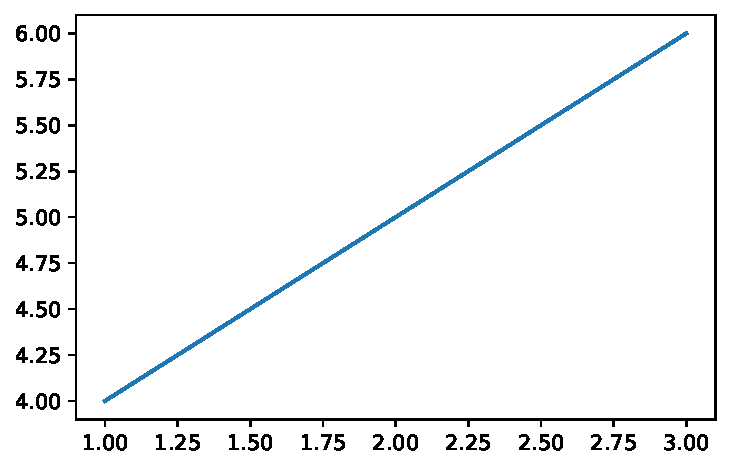
\includegraphics{09_Libraries_files/figure-pdf/cell-8-output-1.pdf}

}

\end{figure}

\begin{tcolorbox}[enhanced jigsaw, coltitle=black, colback=white, bottomrule=.15mm, arc=.35mm, titlerule=0mm, opacitybacktitle=0.6, toptitle=1mm, left=2mm, toprule=.15mm, opacityback=0, bottomtitle=1mm, title=\textcolor{quarto-callout-note-color}{\faInfo}\hspace{0.5em}{Installing \texttt{matplotlib}}, rightrule=.15mm, colframe=quarto-callout-note-color-frame, breakable, colbacktitle=quarto-callout-note-color!10!white, leftrule=.75mm]

Most installs of Python do not include \texttt{matplotlib} as a base
library. You may need to install it. Open up a terminal. Run the
following code to install \texttt{matplotlib}.

\begin{Shaded}
\begin{Highlighting}[]
\ExtensionTok{pip}\NormalTok{ install matplotlib }\AttributeTok{{-}{-}user}
\end{Highlighting}
\end{Shaded}

Note that if you are using a virtual environment, you will need to make
sure the virtual environment is activated first.

\end{tcolorbox}

\hypertarget{importing-modules-from-a-package}{%
\subsubsection{Importing Modules from a
Package}\label{importing-modules-from-a-package}}

Python also supports importing modules from a package, which is a
collection of modules organized under a common namespace. Packages help
in organizing related modules and can be imported similarly to regular
modules.

\textbf{Example: Importing from a Package}

\begin{Shaded}
\begin{Highlighting}[]
\ImportTok{from}\NormalTok{ os }\ImportTok{import}\NormalTok{ path}

\CommentTok{\# Using the path module from the os package}
\BuiltInTok{print}\NormalTok{(path.exists(}\StringTok{"example.txt"}\NormalTok{)) }
\end{Highlighting}
\end{Shaded}

\begin{verbatim}
False
\end{verbatim}

In this example, the \texttt{path} module is imported from the
\texttt{os} package, and its \texttt{exists} function is used to check
if a file exists. Packages are an essential part of Python's ecosystem,
allowing you to organize and distribute your code effectively.

\hypertarget{built-in-libraries}{%
\section{Built-in Libraries}\label{built-in-libraries}}

Python comes with a rich set of built-in libraries that cover a wide
range of functionalities, from mathematical operations to file handling
and beyond. Let's explore a few common libraries that you will
frequently use in your programming journey.

\hypertarget{the-math-library}{%
\paragraph{\texorpdfstring{The \texttt{math}
Library}{The math Library}}\label{the-math-library}}

As you have already seen, the \texttt{math} library provides
mathematical functions and constants.

\textbf{Example: Basic Usage of \texttt{math} Library}

\begin{Shaded}
\begin{Highlighting}[]
\ImportTok{import}\NormalTok{ math}

\CommentTok{\# Using constants}
\BuiltInTok{print}\NormalTok{(math.pi)}

\CommentTok{\# Using functions}
\BuiltInTok{print}\NormalTok{(math.factorial(}\DecValTok{5}\NormalTok{))}
\BuiltInTok{print}\NormalTok{(math.sqrt(}\DecValTok{25}\NormalTok{))}
\end{Highlighting}
\end{Shaded}

\begin{verbatim}
3.141592653589793
120
5.0
\end{verbatim}

\hypertarget{the-random-library}{%
\subsubsection{\texorpdfstring{The \texttt{random}
Library}{The random Library}}\label{the-random-library}}

The \texttt{random} library is used for generating random numbers and
making random selections.

\textbf{Example: Using \texttt{random} Library}

\begin{Shaded}
\begin{Highlighting}[]
\ImportTok{import}\NormalTok{ random}

\CommentTok{\# Generating a random number between 1 and 10}
\BuiltInTok{print}\NormalTok{(random.randint(}\DecValTok{1}\NormalTok{, }\DecValTok{10}\NormalTok{))  }

\CommentTok{\# Picking a random choice from a list}
\NormalTok{choices }\OperatorTok{=}\NormalTok{ [}\StringTok{\textquotesingle{}apple\textquotesingle{}}\NormalTok{, }\StringTok{\textquotesingle{}banana\textquotesingle{}}\NormalTok{, }\StringTok{\textquotesingle{}cherry\textquotesingle{}}\NormalTok{]}
\BuiltInTok{print}\NormalTok{(random.choice(choices)) }
\end{Highlighting}
\end{Shaded}

\begin{verbatim}
8
banana
\end{verbatim}

This library is particularly useful in simulations, games, and scenarios
where randomness is needed.

\hypertarget{creating-custom-modules}{%
\section{Creating Custom Modules}\label{creating-custom-modules}}

Creating your own modules allows you to encapsulate code that can be
reused across multiple projects. As you progress in your coding journey,
you'll find this practice invaluable for maintaining clean and organized
code.

\textbf{Example: Building a Utility Module}

Let's create a module named \texttt{utils.py} that contains some utility
functions:

\begin{Shaded}
\begin{Highlighting}[]
\CommentTok{\# utils.py}

\KeywordTok{def}\NormalTok{ reverse\_string(s):}
    \CommentTok{"""Reverse a given string."""}
    \ControlFlowTok{return}\NormalTok{ s[::}\OperatorTok{{-}}\DecValTok{1}\NormalTok{]}

\KeywordTok{def}\NormalTok{ is\_palindrome(s):}
    \CommentTok{"""Check if a string is a palindrome."""}
    \ControlFlowTok{return}\NormalTok{ s }\OperatorTok{==}\NormalTok{ s[::}\OperatorTok{{-}}\DecValTok{1}\NormalTok{]}
\end{Highlighting}
\end{Shaded}

You can now import and use these functions in any script:

\begin{Shaded}
\begin{Highlighting}[]
\CommentTok{\# main.py}

\ImportTok{import}\NormalTok{ utils}

\NormalTok{word }\OperatorTok{=} \StringTok{"level"}
\BuiltInTok{print}\NormalTok{(utils.reverse\_string(word)) }
\BuiltInTok{print}\NormalTok{(utils.is\_palindrome(word))  }
\end{Highlighting}
\end{Shaded}

\begin{verbatim}
level
True
\end{verbatim}

\hypertarget{best-practices-for-modules-and-libraries}{%
\section{Best Practices for Modules and
Libraries}\label{best-practices-for-modules-and-libraries}}

When working with modules and libraries in Python, following best
practices is essential for creating code that is both maintainable and
user-friendly. One of the most important practices is to use descriptive
names for your modules. The name of a module should clearly convey its
purpose and functionality, making it easier for others (and yourself) to
understand what the module does at a glance. For example, a module named
\texttt{math\_operations} is far more informative than a generic name
like \texttt{utils}, as it immediately indicates that the module
contains functions related to mathematical operations. Descriptive
naming helps prevent confusion, especially in larger projects where
multiple modules are used.

In addition to naming, keeping functions within a module focused on a
single, well-defined task is crucial. Each function should do one thing
and do it well. This approach not only makes your code easier to test
and debug but also enhances its reusability. For instance, a function
that calculates the average of a list of numbers should not also be
responsible for reading the numbers from a file. By adhering to the
principle of single responsibility, you ensure that each function is
modular, making it easier to mix and match functions across different
modules and projects.

Documentation is another critical aspect of writing good modules.
Providing clear and comprehensive docstrings for your modules,
functions, and classes is essential for making your code accessible to
others. Docstrings should explain what the code does, how to use it, and
any important details that users need to be aware of. Well-documented
code not only helps others understand and use your modules but also
serves as a valuable reference for yourself when you return to the code
after some time. Good documentation is a sign of professionalism and
care in coding, making your work more reliable and easier to maintain.

Finally, it is important to avoid side effects in your modules. Side
effects occur when a module executes code automatically upon being
imported, such as modifying global variables or performing I/O
operations. This can lead to unpredictable behavior and bugs, especially
if the user is unaware of these side effects. To prevent this, modules
should generally be passive, only providing functions and classes
without executing any code unless explicitly intended.

\hypertarget{exercises-5}{%
\section{Exercises}\label{exercises-5}}

\hypertarget{excersice-1-creating-a-module}{%
\subsubsection{Excersice 1: Creating a
Module}\label{excersice-1-creating-a-module}}

Create a module \texttt{arithmetic.py} that contains functions for
addition, subtraction, multiplication, and division. Write a script that
imports this module and performs these operations on user-provided
inputs.

\hypertarget{excersice-2-using-built-in-libraries}{%
\subsubsection{Excersice 2: Using Built-in
Libraries}\label{excersice-2-using-built-in-libraries}}

Write a script that uses the \texttt{random} library to generate a
random integer and then uses the \texttt{math} library to find the
square root of this integer.

\hypertarget{excersice-3-module-composition}{%
\subsubsection{Excersice 3: Module
Composition}\label{excersice-3-module-composition}}

Create a module \texttt{geometry.py} that contains functions to
calculate the area and perimeter of different shapes, such as
rectangles, circles, and triangles. Write a script that imports this
module and allows the user to input the dimensions of a shape, then
outputs the calculated area and perimeter.

\hypertarget{excersice-4-creating-a-custom-math-library}{%
\subsubsection{Excersice 4: Creating a Custom Math
Library}\label{excersice-4-creating-a-custom-math-library}}

Develop a custom math module \texttt{custom\_math.py} that includes
functions for basic arithmetic operations, factorial calculation, and
prime number checking. Extend the module by adding a function to
calculate the greatest common divisor (GCD) of two numbers. Write a
script to demonstrate the usage of each function in the module.

\bookmarksetup{startatroot}

\hypertarget{sec-data1}{%
\chapter{Data Structures: Lists and Tuples}\label{sec-data1}}

In the previous chapters, we introduced the basic elements of
programming in Python, including variables, data types, control
structures, and functions. Now, we turn our attention to an essential
topic in computing --- data structures. Data structures allow us to
organize and store data in ways that enable efficient access and
modification. In this chapter, we will explore two foundational data
structures in Python: \textbf{Lists} and \textbf{Tuples}.

\hypertarget{lists}{%
\section{Lists}\label{lists}}

In Python, \textbf{lists} are one of the most commonly used data
structures due to their flexibility and ease of use. A list is a
\textbf{mutable}, \textbf{ordered} collection of elements, which means
the elements in a list can be changed after the list is created, and
they are stored in a specific order. This makes lists ideal for storing
sequences of data that might need to be altered during the execution of
a program.

\hypertarget{creating-lists}{%
\subsection{Creating Lists}\label{creating-lists}}

Lists in Python are defined using square brackets (\texttt{{[}{]}}),
with each element separated by a comma. A list can contain elements of
any data type, including integers, floats, strings, Booleans, and even
other lists.

\textbf{Examples:}

\begin{Shaded}
\begin{Highlighting}[]
\CommentTok{\# A list of integers}
\NormalTok{integer\_list }\OperatorTok{=}\NormalTok{ [}\DecValTok{1}\NormalTok{, }\DecValTok{2}\NormalTok{, }\DecValTok{3}\NormalTok{, }\DecValTok{4}\NormalTok{, }\DecValTok{5}\NormalTok{]}

\CommentTok{\# A list of mixed data types}
\NormalTok{mixed\_list }\OperatorTok{=}\NormalTok{ [}\DecValTok{42}\NormalTok{, }\StringTok{"apple"}\NormalTok{, }\FloatTok{3.14}\NormalTok{, }\VariableTok{True}\NormalTok{]}

\CommentTok{\# A list of lists}
\NormalTok{lists\_list }\OperatorTok{=}\NormalTok{ [integer\_list, mixed\_list]}
\end{Highlighting}
\end{Shaded}

The flexibility of lists allows you to store a wide variety of data in a
single collection, making them useful in many programming contexts, such
as storing records, handling input, and building dynamic datasets.

\hypertarget{accessing-elements-in-a-list}{%
\subsection{Accessing Elements in a
List}\label{accessing-elements-in-a-list}}

Each element in a list is associated with an \textbf{index}---an integer
representing the element's position in the list. In Python, indices
start at 0, meaning the first element is accessed with index \texttt{0},
the second element with index \texttt{1}, and so on. Negative indices
can also be used to access elements from the end of the list, with
\texttt{-1} referring to the last element, \texttt{-2} to the
second-to-last, and so on.

\textbf{Examples:}

\begin{Shaded}
\begin{Highlighting}[]
\CommentTok{\# Accessing elements by positive index}
\NormalTok{my\_list }\OperatorTok{=}\NormalTok{ [}\DecValTok{10}\NormalTok{, }\DecValTok{20}\NormalTok{, }\DecValTok{30}\NormalTok{, }\DecValTok{40}\NormalTok{]}
\BuiltInTok{print}\NormalTok{(my\_list[}\DecValTok{0}\NormalTok{])  }\CommentTok{\# Output: 10}
\BuiltInTok{print}\NormalTok{(my\_list[}\DecValTok{2}\NormalTok{])  }\CommentTok{\# Output: 30}

\CommentTok{\# Accessing elements by negative index}
\BuiltInTok{print}\NormalTok{(my\_list[}\OperatorTok{{-}}\DecValTok{1}\NormalTok{])  }\CommentTok{\# Output: 40}
\BuiltInTok{print}\NormalTok{(my\_list[}\OperatorTok{{-}}\DecValTok{2}\NormalTok{])  }\CommentTok{\# Output: 30}
\end{Highlighting}
\end{Shaded}

\begin{verbatim}
10
30
40
30
\end{verbatim}

\hypertarget{modifying-lists}{%
\subsection{Modifying Lists}\label{modifying-lists}}

One of the most powerful features of lists is their mutability. This
means that after a list is created, its elements can be changed, added,
or removed without creating a new list. There are several ways to modify
lists in Python.

\hypertarget{changing-elements}{%
\subsubsection{Changing Elements}\label{changing-elements}}

You can change individual elements in a list by assigning a new value to
a specific index:

\begin{Shaded}
\begin{Highlighting}[]
\NormalTok{my\_list }\OperatorTok{=}\NormalTok{ [}\DecValTok{1}\NormalTok{, }\DecValTok{2}\NormalTok{, }\DecValTok{3}\NormalTok{]}
\NormalTok{my\_list[}\DecValTok{1}\NormalTok{] }\OperatorTok{=} \DecValTok{99}  
\BuiltInTok{print}\NormalTok{(my\_list)  }
\end{Highlighting}
\end{Shaded}

\begin{verbatim}
[1, 99, 3]
\end{verbatim}

\hypertarget{adding-elements}{%
\subsubsection{Adding Elements}\label{adding-elements}}

You can add elements to a list using the \texttt{append()} method (to
add a single element) or the \texttt{extend()} method (to add multiple
elements):

\begin{Shaded}
\begin{Highlighting}[]
\CommentTok{\# Adding a single element}
\NormalTok{my\_list }\OperatorTok{=}\NormalTok{ [}\DecValTok{1}\NormalTok{, }\DecValTok{2}\NormalTok{, }\DecValTok{3}\NormalTok{]}
\NormalTok{my\_list.append(}\DecValTok{4}\NormalTok{)}
\BuiltInTok{print}\NormalTok{(my\_list)}

\CommentTok{\# Adding multiple elements}
\NormalTok{my\_list.extend([}\DecValTok{5}\NormalTok{, }\DecValTok{6}\NormalTok{])}
\BuiltInTok{print}\NormalTok{(my\_list)}
\end{Highlighting}
\end{Shaded}

\begin{verbatim}
[1, 2, 3, 4]
[1, 2, 3, 4, 5, 6]
\end{verbatim}

You can also use the \texttt{insert()} method to add an element at a
specific index:

\begin{Shaded}
\begin{Highlighting}[]
\NormalTok{my\_list }\OperatorTok{=}\NormalTok{ [}\DecValTok{1}\NormalTok{, }\DecValTok{2}\NormalTok{, }\DecValTok{3}\NormalTok{]}
\NormalTok{my\_list.insert(}\DecValTok{1}\NormalTok{, }\StringTok{"new"}\NormalTok{)}
\BuiltInTok{print}\NormalTok{(my\_list)  }
\end{Highlighting}
\end{Shaded}

\begin{verbatim}
[1, 'new', 2, 3]
\end{verbatim}

\begin{tcolorbox}[enhanced jigsaw, coltitle=black, colback=white, bottomrule=.15mm, arc=.35mm, titlerule=0mm, opacitybacktitle=0.6, toptitle=1mm, left=2mm, toprule=.15mm, opacityback=0, bottomtitle=1mm, title=\textcolor{quarto-callout-note-color}{\faInfo}\hspace{0.5em}{Note}, rightrule=.15mm, colframe=quarto-callout-note-color-frame, breakable, colbacktitle=quarto-callout-note-color!10!white, leftrule=.75mm]

In Python, a \textbf{method} is a function that is associated with an
object. Every method is a function, but not every function is a method.
The key difference is that methods are called on objects, and they are
designed to perform actions related to those objects. The syntax for
calling a method involves the dot notation, where you first specify the
object and then call the method.

Methods are tightly bound to the object they belong to and often
manipulate or interact with the data stored in the object. Python has
built-in methods for its standard data types like lists, strings,
dictionaries, etc.

\end{tcolorbox}

\hypertarget{removing-elements}{%
\subsubsection{Removing Elements}\label{removing-elements}}

Elements can be removed from a list using the \texttt{remove()} method
(to remove the first occurrence of a specific element) or the
\texttt{pop()} method (to remove an element by its index):

\begin{Shaded}
\begin{Highlighting}[]
\CommentTok{\# Removing an element by value}
\NormalTok{my\_list }\OperatorTok{=}\NormalTok{ [}\DecValTok{1}\NormalTok{, }\DecValTok{2}\NormalTok{, }\DecValTok{3}\NormalTok{, }\DecValTok{2}\NormalTok{]}
\NormalTok{my\_list.remove(}\DecValTok{2}\NormalTok{)}
\BuiltInTok{print}\NormalTok{(my\_list)  }

\CommentTok{\# Removing an element by index}
\NormalTok{my\_list.pop(}\DecValTok{1}\NormalTok{) }\CommentTok{\#note that this returns the value being removed}
\BuiltInTok{print}\NormalTok{(my\_list)}
\end{Highlighting}
\end{Shaded}

\begin{verbatim}
[1, 3, 2]
[1, 2]
\end{verbatim}

To clear all elements from a list, use the \texttt{clear()} method:

\begin{Shaded}
\begin{Highlighting}[]
\NormalTok{my\_list }\OperatorTok{=}\NormalTok{ [}\DecValTok{1}\NormalTok{, }\DecValTok{2}\NormalTok{, }\DecValTok{3}\NormalTok{]}
\NormalTok{my\_list.clear()}
\BuiltInTok{print}\NormalTok{(my\_list)}
\end{Highlighting}
\end{Shaded}

\begin{verbatim}
[]
\end{verbatim}

\hypertarget{slicing-lists}{%
\subsection{Slicing Lists}\label{slicing-lists}}

In addition to accessing individual elements, Python allows you to
\textbf{slice} lists, which means extracting a portion of the list to
create a new list. Slicing is done using the colon (\texttt{:})
operator, with the format \texttt{list{[}start:end{]}}. The
\texttt{start} index is inclusive, while the \texttt{end} index is
exclusive.

\textbf{Examples:}

\begin{Shaded}
\begin{Highlighting}[]
\NormalTok{my\_list }\OperatorTok{=}\NormalTok{ [}\DecValTok{10}\NormalTok{, }\DecValTok{20}\NormalTok{, }\DecValTok{30}\NormalTok{, }\DecValTok{40}\NormalTok{, }\DecValTok{50}\NormalTok{]}

\CommentTok{\# Extract elements from index 1 to 3 (2nd to 4th elements)}
\BuiltInTok{print}\NormalTok{(my\_list[}\DecValTok{1}\NormalTok{:}\DecValTok{4}\NormalTok{])  }\CommentTok{\# Output: [20, 30, 40]}

\CommentTok{\# Extract elements from the start to index 3}
\BuiltInTok{print}\NormalTok{(my\_list[:}\DecValTok{4}\NormalTok{])  }\CommentTok{\# Output: [10, 20, 30, 40]}

\CommentTok{\# Extract elements from index 2 to the end}
\BuiltInTok{print}\NormalTok{(my\_list[}\DecValTok{2}\NormalTok{:])  }\CommentTok{\# Output: [30, 40, 50]}
\end{Highlighting}
\end{Shaded}

\begin{verbatim}
[20, 30, 40]
[10, 20, 30, 40]
[30, 40, 50]
\end{verbatim}

Slicing can also be used with a step value, which specifies how many
elements to skip between items:

\begin{Shaded}
\begin{Highlighting}[]
\CommentTok{\# Extract every other element}
\BuiltInTok{print}\NormalTok{(my\_list[::}\DecValTok{2}\NormalTok{]) }
\end{Highlighting}
\end{Shaded}

\begin{verbatim}
[10, 30, 50]
\end{verbatim}

\hypertarget{common-list-operations}{%
\subsection{Common List Operations}\label{common-list-operations}}

Python provides several built-in functions and operators that can be
applied to lists. Below are some of the most commonly used list
operations:

\begin{enumerate}
\def\labelenumi{\arabic{enumi}.}
\item
  \textbf{Checking Length:} You can find the number of elements in a
  list using the \texttt{len()} function:

\begin{Shaded}
\begin{Highlighting}[]
\NormalTok{my\_list }\OperatorTok{=}\NormalTok{ [}\DecValTok{10}\NormalTok{, }\DecValTok{20}\NormalTok{, }\DecValTok{30}\NormalTok{]}
\BuiltInTok{print}\NormalTok{(}\BuiltInTok{len}\NormalTok{(my\_list))}
\end{Highlighting}
\end{Shaded}

\begin{verbatim}
3
\end{verbatim}
\item
  \textbf{Membership Testing:} You can check whether an element is in a
  list using the \texttt{in} keyword:

\begin{Shaded}
\begin{Highlighting}[]
\NormalTok{my\_list }\OperatorTok{=}\NormalTok{ [}\DecValTok{10}\NormalTok{, }\DecValTok{20}\NormalTok{, }\DecValTok{30}\NormalTok{]}
\BuiltInTok{print}\NormalTok{(}\DecValTok{20} \KeywordTok{in}\NormalTok{ my\_list) }
\end{Highlighting}
\end{Shaded}

\begin{verbatim}
True
\end{verbatim}
\item
  \textbf{Sorting Lists:} Lists can be sorted in place using the
  \texttt{sort()} method, or a sorted copy of the list can be returned
  using the \texttt{sorted()} function:

\begin{Shaded}
\begin{Highlighting}[]
\NormalTok{my\_list }\OperatorTok{=}\NormalTok{ [}\DecValTok{3}\NormalTok{, }\DecValTok{1}\NormalTok{, }\DecValTok{4}\NormalTok{, }\DecValTok{1}\NormalTok{, }\DecValTok{5}\NormalTok{, }\DecValTok{9}\NormalTok{]}
\NormalTok{my\_list.sort()  }\CommentTok{\# Sort the list in place}
\BuiltInTok{print}\NormalTok{(my\_list)}
\end{Highlighting}
\end{Shaded}

\begin{verbatim}
[1, 1, 3, 4, 5, 9]
\end{verbatim}
\item
  \textbf{Reversing a List:} You can reverse the order of elements in a
  list using the \texttt{reverse()} method:

\begin{Shaded}
\begin{Highlighting}[]
\NormalTok{my\_list }\OperatorTok{=}\NormalTok{ [}\DecValTok{1}\NormalTok{, }\DecValTok{2}\NormalTok{, }\DecValTok{3}\NormalTok{]}
\NormalTok{my\_list.reverse()}
\BuiltInTok{print}\NormalTok{(my\_list) }
\end{Highlighting}
\end{Shaded}

\begin{verbatim}
[3, 2, 1]
\end{verbatim}
\end{enumerate}

\hypertarget{iterating-over-lists}{%
\subsection{Iterating Over Lists}\label{iterating-over-lists}}

Lists are iterable, which means you can loop through the elements using
a \texttt{for} loop:

\begin{Shaded}
\begin{Highlighting}[]
\NormalTok{my\_list }\OperatorTok{=}\NormalTok{ [}\StringTok{"apple"}\NormalTok{, }\StringTok{"banana"}\NormalTok{, }\StringTok{"cherry"}\NormalTok{]}
\ControlFlowTok{for}\NormalTok{ fruit }\KeywordTok{in}\NormalTok{ my\_list:}
    \BuiltInTok{print}\NormalTok{(fruit)}
\end{Highlighting}
\end{Shaded}

\begin{verbatim}
apple
banana
cherry
\end{verbatim}

You can also iterate over both the index and the element using the
\texttt{enumerate()} function:

\begin{Shaded}
\begin{Highlighting}[]
\NormalTok{my\_list }\OperatorTok{=}\NormalTok{ [}\StringTok{"apple"}\NormalTok{, }\StringTok{"banana"}\NormalTok{, }\StringTok{"cherry"}\NormalTok{]}
\ControlFlowTok{for}\NormalTok{ index, fruit }\KeywordTok{in} \BuiltInTok{enumerate}\NormalTok{(my\_list):}
    \BuiltInTok{print}\NormalTok{(}\SpecialStringTok{f"Index }\SpecialCharTok{\{}\NormalTok{index}\SpecialCharTok{\}}\SpecialStringTok{: }\SpecialCharTok{\{}\NormalTok{fruit}\SpecialCharTok{\}}\SpecialStringTok{"}\NormalTok{)}
\end{Highlighting}
\end{Shaded}

\hypertarget{nesting-lists}{%
\subsubsection{Nesting Lists}\label{nesting-lists}}

Lists can contain other lists as elements, allowing you to create more
complex data structures like matrices or grids. This is known as
\textbf{nesting}.

\textbf{Example:}

\begin{Shaded}
\begin{Highlighting}[]
\NormalTok{matrix }\OperatorTok{=}\NormalTok{ [[}\DecValTok{1}\NormalTok{, }\DecValTok{2}\NormalTok{, }\DecValTok{3}\NormalTok{], [}\DecValTok{4}\NormalTok{, }\DecValTok{5}\NormalTok{, }\DecValTok{6}\NormalTok{], [}\DecValTok{7}\NormalTok{, }\DecValTok{8}\NormalTok{, }\DecValTok{9}\NormalTok{]]}

\CommentTok{\# Accessing the second element of the first list}
\BuiltInTok{print}\NormalTok{(matrix[}\DecValTok{0}\NormalTok{][}\DecValTok{1}\NormalTok{])  }\CommentTok{\# Output: 2}

\CommentTok{\# Iterating over nested lists}
\ControlFlowTok{for}\NormalTok{ row }\KeywordTok{in}\NormalTok{ matrix:}
    \BuiltInTok{print}\NormalTok{(row)}
\end{Highlighting}
\end{Shaded}

\begin{verbatim}
2
[1, 2, 3]
[4, 5, 6]
[7, 8, 9]
\end{verbatim}

\hypertarget{lists-and-built-in-libraries}{%
\subsubsection{Lists and Built-in
Libraries}\label{lists-and-built-in-libraries}}

Lists can be used effectively with common Python libraries. For example,
the \texttt{random} module allows for random selection of elements from
a list:

\textbf{Example:}

\begin{Shaded}
\begin{Highlighting}[]
\ImportTok{import}\NormalTok{ random}

\NormalTok{fruits }\OperatorTok{=}\NormalTok{ [}\StringTok{"apple"}\NormalTok{, }\StringTok{"banana"}\NormalTok{, }\StringTok{"cherry"}\NormalTok{, }\StringTok{"date"}\NormalTok{]}
\BuiltInTok{print}\NormalTok{(random.choice(fruits))  }\CommentTok{\# Randomly selects and prints one fruit}
\end{Highlighting}
\end{Shaded}

\begin{verbatim}
date
\end{verbatim}

\hypertarget{tuples}{%
\section{Tuples}\label{tuples}}

While \textbf{lists} offer flexibility through their mutability, Python
also provides \textbf{tuples}, which are similar in structure but
\textbf{immutable}. Once a tuple is created, its elements cannot be
changed. This immutability makes tuples useful for representing fixed
collections of items that should not or cannot change throughout the
execution of a program. Tuples are ideal when you need to ensure data
integrity, such as coordinates, configuration settings, or when passing
multiple values from functions where immutability is expected.

\hypertarget{creating-tuples}{%
\subsection{Creating Tuples}\label{creating-tuples}}

Tuples are defined using parentheses \texttt{()} and can hold elements
of any data type, much like lists. However, since they are immutable,
you cannot modify the elements of a tuple after it is created.

\textbf{Syntax:}

\begin{Shaded}
\begin{Highlighting}[]
\CommentTok{\# Creating a tuple}
\NormalTok{my\_tuple }\OperatorTok{=}\NormalTok{ (}\DecValTok{10}\NormalTok{, }\DecValTok{20}\NormalTok{, }\DecValTok{30}\NormalTok{)}
\end{Highlighting}
\end{Shaded}

It's also possible to create tuples without using parentheses, though
this is less common:

\begin{Shaded}
\begin{Highlighting}[]
\NormalTok{my\_tuple }\OperatorTok{=} \DecValTok{10}\NormalTok{, }\DecValTok{20}\NormalTok{, }\DecValTok{30}
\end{Highlighting}
\end{Shaded}

Tuples can contain elements of different types:

\begin{Shaded}
\begin{Highlighting}[]
\NormalTok{mixed\_tuple }\OperatorTok{=}\NormalTok{ (}\DecValTok{1}\NormalTok{, }\StringTok{"apple"}\NormalTok{, }\FloatTok{3.14}\NormalTok{, }\VariableTok{True}\NormalTok{)}
\end{Highlighting}
\end{Shaded}

Tuples with a single element need to have a comma after the element to
avoid confusion with parentheses used in expressions:

\begin{Shaded}
\begin{Highlighting}[]
\NormalTok{single\_element\_tuple }\OperatorTok{=}\NormalTok{ (}\DecValTok{5}\NormalTok{,)}
\BuiltInTok{print}\NormalTok{(}\BuiltInTok{type}\NormalTok{(single\_element\_tuple))}
\end{Highlighting}
\end{Shaded}

\begin{verbatim}
<class 'tuple'>
\end{verbatim}

\hypertarget{accessing-tuple-elements}{%
\subsection{Accessing Tuple Elements}\label{accessing-tuple-elements}}

Like lists, tuples are indexed starting at 0, and individual elements
can be accessed using their index. However, since tuples are immutable,
you cannot modify their elements.

\textbf{Examples:}

\begin{Shaded}
\begin{Highlighting}[]
\NormalTok{my\_tuple }\OperatorTok{=}\NormalTok{ (}\DecValTok{10}\NormalTok{, }\DecValTok{20}\NormalTok{, }\DecValTok{30}\NormalTok{, }\DecValTok{40}\NormalTok{)}

\CommentTok{\# Accessing the first element}
\BuiltInTok{print}\NormalTok{(my\_tuple[}\DecValTok{0}\NormalTok{]) }

\CommentTok{\# Accessing the last element using negative indexing}
\BuiltInTok{print}\NormalTok{(my\_tuple[}\OperatorTok{{-}}\DecValTok{1}\NormalTok{]) }
\end{Highlighting}
\end{Shaded}

\begin{verbatim}
10
40
\end{verbatim}

You can slice tuples just like lists, returning a new tuple containing
the specified range of elements:

\begin{Shaded}
\begin{Highlighting}[]
\CommentTok{\# Slicing a tuple}
\BuiltInTok{print}\NormalTok{(my\_tuple[}\DecValTok{1}\NormalTok{:}\DecValTok{3}\NormalTok{]) }
\end{Highlighting}
\end{Shaded}

\begin{verbatim}
(20, 30)
\end{verbatim}

\hypertarget{tuple-operations}{%
\subsection{Tuple Operations}\label{tuple-operations}}

Although tuples are immutable, there are still several operations you
can perform on them:

\begin{enumerate}
\def\labelenumi{\arabic{enumi}.}
\item
  \textbf{Length of a Tuple:} You can find the number of elements in a
  tuple using the \texttt{len()} function:

\begin{Shaded}
\begin{Highlighting}[]
\NormalTok{my\_tuple }\OperatorTok{=}\NormalTok{ (}\DecValTok{10}\NormalTok{, }\DecValTok{20}\NormalTok{, }\DecValTok{30}\NormalTok{)}
\BuiltInTok{print}\NormalTok{(}\BuiltInTok{len}\NormalTok{(my\_tuple))  }
\end{Highlighting}
\end{Shaded}

\begin{verbatim}
3
\end{verbatim}
\item
  \textbf{Membership Testing:} Use the \texttt{in} keyword to check
  whether an element exists in a tuple:

\begin{Shaded}
\begin{Highlighting}[]
\NormalTok{my\_tuple }\OperatorTok{=}\NormalTok{ (}\DecValTok{10}\NormalTok{, }\DecValTok{20}\NormalTok{, }\DecValTok{30}\NormalTok{)}
\BuiltInTok{print}\NormalTok{(}\DecValTok{20} \KeywordTok{in}\NormalTok{ my\_tuple)  }
\end{Highlighting}
\end{Shaded}

\begin{verbatim}
True
\end{verbatim}
\item
  \textbf{Iterating Over a Tuple:} Tuples are iterable, so you can loop
  through their elements using a \texttt{for} loop:

\begin{Shaded}
\begin{Highlighting}[]
\ControlFlowTok{for}\NormalTok{ item }\KeywordTok{in}\NormalTok{ my\_tuple:}
    \BuiltInTok{print}\NormalTok{(item)}
\end{Highlighting}
\end{Shaded}

\begin{verbatim}
10
20
30
\end{verbatim}
\item
  \textbf{Indexing and Slicing:} Like lists, tuples support indexing and
  slicing:

\begin{Shaded}
\begin{Highlighting}[]
\NormalTok{my\_tuple }\OperatorTok{=}\NormalTok{ (}\DecValTok{10}\NormalTok{, }\DecValTok{20}\NormalTok{, }\DecValTok{30}\NormalTok{, }\DecValTok{40}\NormalTok{)}
\BuiltInTok{print}\NormalTok{(my\_tuple[}\DecValTok{1}\NormalTok{:}\DecValTok{3}\NormalTok{])  }
\end{Highlighting}
\end{Shaded}

\begin{verbatim}
(20, 30)
\end{verbatim}
\end{enumerate}

\hypertarget{nested-tuples}{%
\subsection{Nested Tuples}\label{nested-tuples}}

Tuples can be \textbf{nested} inside other tuples, allowing you to
create multi-level data structures. This is useful when organizing
complex data, such as in multidimensional arrays or coordinate systems.

\textbf{Example:}

\begin{Shaded}
\begin{Highlighting}[]
\NormalTok{nested\_tuple }\OperatorTok{=}\NormalTok{ ((}\DecValTok{1}\NormalTok{, }\DecValTok{2}\NormalTok{), (}\DecValTok{3}\NormalTok{, }\DecValTok{4}\NormalTok{), (}\DecValTok{5}\NormalTok{, }\DecValTok{6}\NormalTok{))}

\CommentTok{\# Accessing the first tuple}
\BuiltInTok{print}\NormalTok{(nested\_tuple[}\DecValTok{0}\NormalTok{])  }

\CommentTok{\# Accessing an element from a nested tuple}
\BuiltInTok{print}\NormalTok{(nested\_tuple[}\DecValTok{0}\NormalTok{][}\DecValTok{1}\NormalTok{])  }
\end{Highlighting}
\end{Shaded}

\begin{verbatim}
(1, 2)
2
\end{verbatim}

\hypertarget{unpacking-tuples}{%
\subsection{Unpacking Tuples}\label{unpacking-tuples}}

One of the most powerful features of tuples is \textbf{tuple unpacking},
which allows you to assign the elements of a tuple to individual
variables in a single statement.

\textbf{Example:}

\begin{Shaded}
\begin{Highlighting}[]
\CommentTok{\# Unpacking a tuple into variables}
\NormalTok{coordinates }\OperatorTok{=}\NormalTok{ (}\DecValTok{10}\NormalTok{, }\DecValTok{20}\NormalTok{)}
\NormalTok{x, y }\OperatorTok{=}\NormalTok{ coordinates}
\BuiltInTok{print}\NormalTok{(x)  }
\BuiltInTok{print}\NormalTok{(y)  }
\end{Highlighting}
\end{Shaded}

\begin{verbatim}
10
20
\end{verbatim}

Tuple unpacking is especially useful when functions return multiple
values in a tuple, allowing you to capture and work with these values
directly.

\textbf{Example:}

\begin{Shaded}
\begin{Highlighting}[]
\KeywordTok{def}\NormalTok{ rectangle\_properties(length, width):}
\NormalTok{    area }\OperatorTok{=}\NormalTok{ length }\OperatorTok{*}\NormalTok{ width}
\NormalTok{    perimeter }\OperatorTok{=} \DecValTok{2} \OperatorTok{*}\NormalTok{ (length }\OperatorTok{+}\NormalTok{ width)}
    \ControlFlowTok{return}\NormalTok{ (area, perimeter)}

\CommentTok{\# Unpacking the returned tuple into variables}
\NormalTok{area, perimeter }\OperatorTok{=}\NormalTok{ rectangle\_properties(}\DecValTok{5}\NormalTok{, }\DecValTok{10}\NormalTok{)}
\BuiltInTok{print}\NormalTok{(}\SpecialStringTok{f"Area: }\SpecialCharTok{\{}\NormalTok{area}\SpecialCharTok{\}}\SpecialStringTok{, Perimeter: }\SpecialCharTok{\{}\NormalTok{perimeter}\SpecialCharTok{\}}\SpecialStringTok{"}\NormalTok{)}
\end{Highlighting}
\end{Shaded}

\begin{verbatim}
Area: 50, Perimeter: 30
\end{verbatim}

\hypertarget{tuple-methods}{%
\subsection{Tuple Methods}\label{tuple-methods}}

Since tuples are immutable, they have fewer methods compared to lists.
However, they do provide two useful methods:

\begin{enumerate}
\def\labelenumi{\arabic{enumi}.}
\item
  \textbf{count()}: Returns the number of times a specified value
  appears in the tuple.

\begin{Shaded}
\begin{Highlighting}[]
\NormalTok{my\_tuple }\OperatorTok{=}\NormalTok{ (}\DecValTok{1}\NormalTok{, }\DecValTok{2}\NormalTok{, }\DecValTok{2}\NormalTok{, }\DecValTok{3}\NormalTok{, }\DecValTok{2}\NormalTok{)}
\BuiltInTok{print}\NormalTok{(my\_tuple.count(}\DecValTok{2}\NormalTok{))  }
\end{Highlighting}
\end{Shaded}

\begin{verbatim}
3
\end{verbatim}
\item
  \textbf{index()}: Returns the index of the first occurrence of a
  specified value.

\begin{Shaded}
\begin{Highlighting}[]
\NormalTok{my\_tuple }\OperatorTok{=}\NormalTok{ (}\DecValTok{1}\NormalTok{, }\DecValTok{2}\NormalTok{, }\DecValTok{3}\NormalTok{)}
\BuiltInTok{print}\NormalTok{(my\_tuple.index(}\DecValTok{2}\NormalTok{)) }
\end{Highlighting}
\end{Shaded}

\begin{verbatim}
1
\end{verbatim}
\end{enumerate}

\hypertarget{list-comprehension}{%
\section{List Comprehension}\label{list-comprehension}}

In Python, \textbf{list comprehension} provides a concise way to
generate lists. It offers a more readable and often more efficient
alternative to using loops and \texttt{append()} to build lists. List
comprehension allows you to apply an expression to each element in a
sequence and optionally include conditional statements to filter
elements. This compact syntax makes it easy to create lists based on
existing sequences or from operations.

\hypertarget{basic-syntax-of-list-comprehension}{%
\subsection{Basic Syntax of List
Comprehension}\label{basic-syntax-of-list-comprehension}}

The basic syntax of list comprehension is:

\begin{Shaded}
\begin{Highlighting}[]
\NormalTok{[expression }\ControlFlowTok{for}\NormalTok{ item }\KeywordTok{in}\NormalTok{ iterable]}
\end{Highlighting}
\end{Shaded}

\begin{itemize}
\tightlist
\item
  \texttt{expression}: This is the operation or value you want to apply
  to each item in the iterable.
\item
  \texttt{item}: Each element from the iterable (e.g., a list, tuple, or
  string).
\item
  \texttt{iterable}: The sequence of elements to loop over (e.g., a
  list, range, or other iterable object).
\end{itemize}

This simple form of list comprehension generates a new list by
evaluating the expression for each element in the iterable.

\textbf{Example: Creating a list of squares}

\begin{Shaded}
\begin{Highlighting}[]
\NormalTok{squares }\OperatorTok{=}\NormalTok{ [x}\OperatorTok{**}\DecValTok{2} \ControlFlowTok{for}\NormalTok{ x }\KeywordTok{in} \BuiltInTok{range}\NormalTok{(}\DecValTok{5}\NormalTok{)]}
\BuiltInTok{print}\NormalTok{(squares) }
\end{Highlighting}
\end{Shaded}

\begin{verbatim}
[0, 1, 4, 9, 16]
\end{verbatim}

In this example, for each value \texttt{x} in \texttt{range(5)}, Python
evaluates \texttt{x**2} and adds the result to the new list. The result
is a list of the squares of the numbers from 0 to 4.

\hypertarget{list-comprehension-with-conditional-logic}{%
\subsection{List Comprehension with Conditional
Logic}\label{list-comprehension-with-conditional-logic}}

List comprehension can include \textbf{conditional logic}, allowing you
to filter elements or apply an operation only when a condition is met.
The syntax for adding a condition is as follows:

\begin{Shaded}
\begin{Highlighting}[]
\NormalTok{[expression }\ControlFlowTok{for}\NormalTok{ item }\KeywordTok{in}\NormalTok{ iterable }\ControlFlowTok{if}\NormalTok{ condition]}
\end{Highlighting}
\end{Shaded}

The \texttt{condition} is a logical statement that is evaluated for each
item in the iterable. Only items for which the condition evaluates to
\texttt{True} are included in the resulting list.

\textbf{Example: Filtering even numbers}

\begin{Shaded}
\begin{Highlighting}[]
\NormalTok{even\_numbers }\OperatorTok{=}\NormalTok{ [x }\ControlFlowTok{for}\NormalTok{ x }\KeywordTok{in} \BuiltInTok{range}\NormalTok{(}\DecValTok{10}\NormalTok{) }\ControlFlowTok{if}\NormalTok{ x }\OperatorTok{\%} \DecValTok{2} \OperatorTok{==} \DecValTok{0}\NormalTok{]}
\BuiltInTok{print}\NormalTok{(even\_numbers)  }
\end{Highlighting}
\end{Shaded}

\begin{verbatim}
[0, 2, 4, 6, 8]
\end{verbatim}

Here, only numbers that satisfy the condition \texttt{x\ \%\ 2\ ==\ 0}
(i.e., the even numbers) are included in the resulting list.

You can also use an \texttt{if-else} expression within list
comprehension for more complex logic:

\begin{Shaded}
\begin{Highlighting}[]
\NormalTok{[expression\_if\_true }\ControlFlowTok{if}\NormalTok{ condition }\ControlFlowTok{else}\NormalTok{ expression\_if\_false }\ControlFlowTok{for}\NormalTok{ item }\KeywordTok{in}\NormalTok{ iterable]}
\end{Highlighting}
\end{Shaded}

\textbf{Example: Labeling even and odd numbers}

\begin{Shaded}
\begin{Highlighting}[]
\NormalTok{labels }\OperatorTok{=}\NormalTok{ [}\StringTok{"even"} \ControlFlowTok{if}\NormalTok{ x }\OperatorTok{\%} \DecValTok{2} \OperatorTok{==} \DecValTok{0} \ControlFlowTok{else} \StringTok{"odd"} \ControlFlowTok{for}\NormalTok{ x }\KeywordTok{in} \BuiltInTok{range}\NormalTok{(}\DecValTok{5}\NormalTok{)]}
\BuiltInTok{print}\NormalTok{(labels)  }
\end{Highlighting}
\end{Shaded}

\begin{verbatim}
['even', 'odd', 'even', 'odd', 'even']
\end{verbatim}

In this case, the comprehension adds the string \texttt{"even"} to the
list if \texttt{x} is divisible by 2 and \texttt{"odd"} otherwise.

\hypertarget{nested-list-comprehension}{%
\subsection{Nested List Comprehension}\label{nested-list-comprehension}}

List comprehension can also be nested to create lists from
multidimensional structures, such as matrices. Nested list
comprehensions are powerful but can become harder to read if not used
carefully.

The basic syntax for nested list comprehension is:

\begin{Shaded}
\begin{Highlighting}[]
\NormalTok{[expression }\ControlFlowTok{for}\NormalTok{ item1 }\KeywordTok{in}\NormalTok{ iterable1 }\ControlFlowTok{for}\NormalTok{ item2 }\KeywordTok{in}\NormalTok{ iterable2]}
\end{Highlighting}
\end{Shaded}

\textbf{Example: Flattening a matrix (a list of lists)}

\begin{Shaded}
\begin{Highlighting}[]
\NormalTok{matrix }\OperatorTok{=}\NormalTok{ [[}\DecValTok{1}\NormalTok{, }\DecValTok{2}\NormalTok{, }\DecValTok{3}\NormalTok{], [}\DecValTok{4}\NormalTok{, }\DecValTok{5}\NormalTok{, }\DecValTok{6}\NormalTok{], [}\DecValTok{7}\NormalTok{, }\DecValTok{8}\NormalTok{, }\DecValTok{9}\NormalTok{]]}
\NormalTok{flat\_list }\OperatorTok{=}\NormalTok{ [num }\ControlFlowTok{for}\NormalTok{ row }\KeywordTok{in}\NormalTok{ matrix }\ControlFlowTok{for}\NormalTok{ num }\KeywordTok{in}\NormalTok{ row]}
\BuiltInTok{print}\NormalTok{(flat\_list) }
\end{Highlighting}
\end{Shaded}

\begin{verbatim}
[1, 2, 3, 4, 5, 6, 7, 8, 9]
\end{verbatim}

In this example, we loop over each row in the matrix, and for each row,
we loop over each number, adding it to a single list
(\texttt{flat\_list}).

\textbf{Example: Multiplying elements in a matrix by 2}

\begin{Shaded}
\begin{Highlighting}[]
\NormalTok{matrix }\OperatorTok{=}\NormalTok{ [[}\DecValTok{1}\NormalTok{, }\DecValTok{2}\NormalTok{, }\DecValTok{3}\NormalTok{], [}\DecValTok{4}\NormalTok{, }\DecValTok{5}\NormalTok{, }\DecValTok{6}\NormalTok{], [}\DecValTok{7}\NormalTok{, }\DecValTok{8}\NormalTok{, }\DecValTok{9}\NormalTok{]]}
\NormalTok{doubled\_matrix }\OperatorTok{=}\NormalTok{ [[num }\OperatorTok{*} \DecValTok{2} \ControlFlowTok{for}\NormalTok{ num }\KeywordTok{in}\NormalTok{ row] }\ControlFlowTok{for}\NormalTok{ row }\KeywordTok{in}\NormalTok{ matrix]}
\BuiltInTok{print}\NormalTok{(doubled\_matrix)}
\end{Highlighting}
\end{Shaded}

\begin{verbatim}
[[2, 4, 6], [8, 10, 12], [14, 16, 18]]
\end{verbatim}

In this case, the list comprehension multiplies each element in the
matrix by 2, resulting in a new matrix where all values are doubled.

\hypertarget{list-comprehension-with-built-in-functions}{%
\subsection{List Comprehension with Built-in
Functions}\label{list-comprehension-with-built-in-functions}}

You can combine list comprehensions with built-in Python functions to
perform more complex transformations and calculations. This is a common
pattern when dealing with operations such as string manipulation,
mathematical calculations, or other functional transformations.

\textbf{Example: Using the \texttt{len()} function}

\begin{Shaded}
\begin{Highlighting}[]
\NormalTok{words }\OperatorTok{=}\NormalTok{ [}\StringTok{"apple"}\NormalTok{, }\StringTok{"banana"}\NormalTok{, }\StringTok{"cherry"}\NormalTok{]}
\NormalTok{word\_lengths }\OperatorTok{=}\NormalTok{ [}\BuiltInTok{len}\NormalTok{(word) }\ControlFlowTok{for}\NormalTok{ word }\KeywordTok{in}\NormalTok{ words]}
\BuiltInTok{print}\NormalTok{(word\_lengths)  }
\end{Highlighting}
\end{Shaded}

\begin{verbatim}
[5, 6, 6]
\end{verbatim}

Here, the list comprehension applies the \texttt{len()} function to each
word in the list \texttt{words}, resulting in a list of the word
lengths.

\textbf{Example: Using \texttt{sum()} with list comprehension} Suppose
we have a list of lists representing test scores for different students.
We can calculate the sum of each student's test scores using list
comprehension:

\begin{Shaded}
\begin{Highlighting}[]
\NormalTok{scores }\OperatorTok{=}\NormalTok{ [[}\DecValTok{75}\NormalTok{, }\DecValTok{80}\NormalTok{, }\DecValTok{85}\NormalTok{], [}\DecValTok{60}\NormalTok{, }\DecValTok{70}\NormalTok{, }\DecValTok{75}\NormalTok{], [}\DecValTok{90}\NormalTok{, }\DecValTok{95}\NormalTok{, }\DecValTok{100}\NormalTok{]]}
\NormalTok{total\_scores }\OperatorTok{=}\NormalTok{ [}\BuiltInTok{sum}\NormalTok{(student\_scores) }\ControlFlowTok{for}\NormalTok{ student\_scores }\KeywordTok{in}\NormalTok{ scores]}
\BuiltInTok{print}\NormalTok{(total\_scores) }
\end{Highlighting}
\end{Shaded}

\begin{verbatim}
[240, 205, 285]
\end{verbatim}

In this example, \texttt{sum()} calculates the total score for each
student, and list comprehension gathers these sums into a new list
\texttt{total\_scores}.

\hypertarget{list-comprehension-vs.-loops}{%
\subsection{List Comprehension
vs.~Loops}\label{list-comprehension-vs.-loops}}

List comprehension is often favored over traditional loops because it
provides a more \textbf{compact} and \textbf{readable} syntax. However,
there are cases where a loop might be more appropriate, especially when
the logic is complex, or when you need to modify elements in place.

\textbf{Example: Traditional loop}

\begin{Shaded}
\begin{Highlighting}[]
\NormalTok{squares }\OperatorTok{=}\NormalTok{ []}
\ControlFlowTok{for}\NormalTok{ x }\KeywordTok{in} \BuiltInTok{range}\NormalTok{(}\DecValTok{5}\NormalTok{):}
\NormalTok{    squares.append(x}\OperatorTok{**}\DecValTok{2}\NormalTok{)}
\BuiltInTok{print}\NormalTok{(squares) }
\end{Highlighting}
\end{Shaded}

\begin{verbatim}
[0, 1, 4, 9, 16]
\end{verbatim}

\textbf{Equivalent list comprehension:}

\begin{Shaded}
\begin{Highlighting}[]
\NormalTok{squares }\OperatorTok{=}\NormalTok{ [x}\OperatorTok{**}\DecValTok{2} \ControlFlowTok{for}\NormalTok{ x }\KeywordTok{in} \BuiltInTok{range}\NormalTok{(}\DecValTok{5}\NormalTok{)]}
\BuiltInTok{print}\NormalTok{(squares)  }
\end{Highlighting}
\end{Shaded}

\begin{verbatim}
[0, 1, 4, 9, 16]
\end{verbatim}

List comprehension is faster for simple operations because it avoids the
overhead of repeatedly calling \texttt{append()} and performing function
calls. However, for more complex logic, such as multiple conditional
statements or nested loops, the clarity of traditional loops might
outweigh the brevity of list comprehension.

\hypertarget{list-comprehension-with-external-libraries}{%
\subsection{List Comprehension with External
Libraries}\label{list-comprehension-with-external-libraries}}

List comprehension can be used effectively with other basic libraries
like \texttt{math} or \texttt{random}.

\textbf{Example: Using \texttt{math.sqrt()} with list comprehension}

\begin{Shaded}
\begin{Highlighting}[]
\ImportTok{import}\NormalTok{ math}
\NormalTok{numbers }\OperatorTok{=}\NormalTok{ [}\DecValTok{1}\NormalTok{, }\DecValTok{4}\NormalTok{, }\DecValTok{9}\NormalTok{, }\DecValTok{16}\NormalTok{, }\DecValTok{25}\NormalTok{]}
\NormalTok{square\_roots }\OperatorTok{=}\NormalTok{ [math.sqrt(num) }\ControlFlowTok{for}\NormalTok{ num }\KeywordTok{in}\NormalTok{ numbers]}
\BuiltInTok{print}\NormalTok{(square\_roots)  }
\end{Highlighting}
\end{Shaded}

\begin{verbatim}
[1.0, 2.0, 3.0, 4.0, 5.0]
\end{verbatim}

In this example, \texttt{math.sqrt()} is applied to each number in the
list \texttt{numbers}, resulting in a list of square roots.

\textbf{Example: Using \texttt{random.randint()}} You can also use list
comprehension with the \texttt{random} module to generate random
numbers:

\begin{Shaded}
\begin{Highlighting}[]
\ImportTok{import}\NormalTok{ random}
\NormalTok{random\_numbers }\OperatorTok{=}\NormalTok{ [random.randint(}\DecValTok{1}\NormalTok{, }\DecValTok{100}\NormalTok{) }\ControlFlowTok{for}\NormalTok{ \_ }\KeywordTok{in} \BuiltInTok{range}\NormalTok{(}\DecValTok{5}\NormalTok{)]}
\BuiltInTok{print}\NormalTok{(random\_numbers)  }
\end{Highlighting}
\end{Shaded}

\begin{verbatim}
[43, 72, 17, 4, 3]
\end{verbatim}

Here, the \texttt{\_} is a placeholder variable (indicating that the
value is not important), and \texttt{random.randint()} generates a
random integer for each iteration.

\hypertarget{limitations-of-list-comprehension}{%
\subsection{Limitations of List
Comprehension}\label{limitations-of-list-comprehension}}

While list comprehension is a powerful tool, there are some cases where
it may not be the best choice:

\begin{itemize}
\item
  \textbf{Readability}: Overusing or nesting list comprehensions can
  make code difficult to read and maintain, especially when working with
  complex logic. In such cases, using traditional loops or helper
  functions might result in clearer and more maintainable code.
\item
  \textbf{Complex operations}: When performing complex operations with
  multiple steps, it's often better to use traditional loops to avoid
  confusion and improve code clarity.
\item
  \textbf{Memory efficiency}: Since list comprehensions create a new
  list in memory, they might not be suitable for extremely large
  datasets. In such cases, consider using generator expressions (which
  we will cover in later sections) to optimize memory usage.
\end{itemize}

\hypertarget{example-practical-applications-of-list-comprehension}{%
\subsection{Example: Practical Applications of List
Comprehension}\label{example-practical-applications-of-list-comprehension}}

To conclude, let's explore a practical application of list comprehension
in data processing.

\textbf{Example: Filtering and transforming data} Suppose we are
processing a list of student scores, and we want to filter out scores
below 50 and increase the remaining scores by 10\%. We can accomplish
this efficiently with list comprehension.

\begin{Shaded}
\begin{Highlighting}[]
\NormalTok{scores }\OperatorTok{=}\NormalTok{ [}\DecValTok{45}\NormalTok{, }\DecValTok{67}\NormalTok{, }\DecValTok{85}\NormalTok{, }\DecValTok{30}\NormalTok{, }\DecValTok{78}\NormalTok{, }\DecValTok{92}\NormalTok{, }\DecValTok{40}\NormalTok{]}
\NormalTok{adjusted\_scores }\OperatorTok{=}\NormalTok{ [score }\OperatorTok{*} \FloatTok{1.1} \ControlFlowTok{for}\NormalTok{ score }\KeywordTok{in}\NormalTok{ scores }\ControlFlowTok{if}\NormalTok{ score }\OperatorTok{\textgreater{}=} \DecValTok{50}\NormalTok{]}
\BuiltInTok{print}\NormalTok{(adjusted\_scores)  }
\end{Highlighting}
\end{Shaded}

\begin{verbatim}
[73.7, 93.50000000000001, 85.80000000000001, 101.2]
\end{verbatim}

In this example, only scores greater than or equal to 50 are included,
and each selected score is increased by 10\%. List comprehension
simplifies the process of filtering and transforming the data in a
single readable line.

\hypertarget{exercises-6}{%
\section{Exercises}\label{exercises-6}}

\hypertarget{excersice-1-basic-list-operations}{%
\subsubsection{Excersice 1: Basic List
Operations}\label{excersice-1-basic-list-operations}}

\begin{enumerate}
\def\labelenumi{\alph{enumi}.}
\tightlist
\item
  Create a list named \texttt{fruits} with the values: ``apple'',
  ``banana'', ``cherry''.\\
\item
  Add the fruit ``orange'' to the list.\\
\item
  Remove ``banana'' from the list.\\
\item
  Print the second fruit in the list.\\
\item
  Print the length of the list.
\end{enumerate}

\hypertarget{excersice-2-modifying-lists}{%
\subsubsection{Excersice 2: Modifying
Lists}\label{excersice-2-modifying-lists}}

\begin{enumerate}
\def\labelenumi{\alph{enumi}.}
\tightlist
\item
  Create a list \texttt{numbers} containing the values 1, 2, 3, 4, and
  5.\\
\item
  Replace the third element in the list with the value 10.\\
\item
  Add the number 6 to the end of the list.\\
\item
  Insert the number 0 at the beginning of the list.\\
\item
  Print the updated list.
\end{enumerate}

\hypertarget{excersice-3-slicing-lists}{%
\subsubsection{Excersice 3: Slicing
Lists}\label{excersice-3-slicing-lists}}

Given the list
\texttt{colors\ =\ {[}"red",\ "green",\ "blue",\ "yellow",\ "purple"{]}},\\
a. Slice and print the first three colors.\\
b. Slice and print the last two colors.\\
c.~Slice and print every second color in the list.

\hypertarget{excersice-4-nested-lists}{%
\subsubsection{Excersice 4: Nested
Lists}\label{excersice-4-nested-lists}}

Create a nested list
\texttt{matrix\ =\ {[}{[}1,\ 2,\ 3{]},\ {[}4,\ 5,\ 6{]},\ {[}7,\ 8,\ 9{]}{]}}.\\
a. Print the element at the first row and second column.\\
b. Change the element at the second row and third column to 10.\\
c.~Print the entire second row.

\hypertarget{excersice-5-basic-tuple-operations}{%
\subsubsection{Excersice 5: Basic Tuple
Operations}\label{excersice-5-basic-tuple-operations}}

\begin{enumerate}
\def\labelenumi{\alph{enumi}.}
\tightlist
\item
  Create a tuple \texttt{my\_tuple} with values: 10, 20, 30, 40, 50.\\
\item
  Print the value at index 2.\\
\item
  Try to change the value at index 1 to 15 (what happens?).\\
\item
  Print the length of the tuple.
\end{enumerate}

\hypertarget{excersice-6-tuple-unpacking}{%
\subsubsection{Excersice 6: Tuple
Unpacking}\label{excersice-6-tuple-unpacking}}

\begin{enumerate}
\def\labelenumi{\alph{enumi}.}
\tightlist
\item
  Create a tuple \texttt{dimensions\ =\ (1920,\ 1080)}.\\
\item
  Unpack the tuple into variables \texttt{width} and \texttt{height}.\\
\item
  Print the values of \texttt{width} and \texttt{height}.
\end{enumerate}

\hypertarget{excersice-7-returning-tuples-from-functions}{%
\subsubsection{Excersice 7: Returning Tuples from
Functions}\label{excersice-7-returning-tuples-from-functions}}

\begin{enumerate}
\def\labelenumi{\alph{enumi}.}
\tightlist
\item
  Write a function \texttt{calculate\_stats(numbers)} that takes a list
  of numbers and returns a tuple containing the sum and the average of
  the list.\\
\item
  Call the function with the list \texttt{{[}10,\ 20,\ 30,\ 40,\ 50{]}}
  and unpack the returned tuple into variables \texttt{total\_sum} and
  \texttt{average}.\\
\item
  Print the values of \texttt{total\_sum} and \texttt{average}.
\end{enumerate}

\hypertarget{excersice-8-nested-tuples}{%
\subsubsection{Excersice 8: Nested
Tuples}\label{excersice-8-nested-tuples}}

Given the nested tuple
\texttt{nested\ =\ ((1,\ 2),\ (3,\ 4),\ (5,\ 6))},\\
a. Print the first element of the second tuple.\\
b. Try to change the second element of the third tuple to 7 (what
happens?).

\hypertarget{excersice-9-basic-list-comprehension}{%
\subsubsection{Excersice 9: Basic List
Comprehension}\label{excersice-9-basic-list-comprehension}}

\begin{enumerate}
\def\labelenumi{\alph{enumi}.}
\tightlist
\item
  Create a list comprehension that generates a list of squares of
  numbers from 1 to 10.\\
\item
  Create a list comprehension that generates a list of even numbers
  between 1 and 20.
\end{enumerate}

\hypertarget{excersice-10-basic-list-comprehension}{%
\subsubsection{Excersice 10: Basic List
Comprehension}\label{excersice-10-basic-list-comprehension}}

\begin{enumerate}
\def\labelenumi{\alph{enumi}.}
\tightlist
\item
  Create a list comprehension that generates a list of all numbers
  between 1 and 50 that are divisible by 3.\\
\item
  Create a list comprehension that generates a list of all numbers
  between 1 and 100 that are divisible by both 2 and 5.
\end{enumerate}

\hypertarget{excersice-11-nested-list-comprehension}{%
\subsubsection{Excersice 11: Nested List
Comprehension}\label{excersice-11-nested-list-comprehension}}

Using nested list comprehension, create a list of all possible
combinations of two numbers, where the first number is from the list
\texttt{{[}1,\ 2,\ 3{]}} and the second number is from the list
\texttt{{[}4,\ 5,\ 6{]}}.

\hypertarget{excersice-12-string-manipulation-with-list-comprehension}{%
\subsubsection{Excersice 12: String Manipulation with List
Comprehension}\label{excersice-12-string-manipulation-with-list-comprehension}}

Given the list
\texttt{words\ =\ {[}"apple",\ "banana",\ "cherry",\ "date"{]}},\\
a. Create a list comprehension that returns the lengths of each word in
the list.\\
b. Create a list comprehension that converts each word in the list to
uppercase.

\hypertarget{excersice-13-tuples-and-list-comprehension}{%
\subsubsection{Excersice 13: Tuples and List
Comprehension}\label{excersice-13-tuples-and-list-comprehension}}

Given a list of tuples representing students and their scores:\\
\texttt{students\ =\ {[}("Alice",\ 85),\ ("Bob",\ 60),\ ("Charlie",\ 95),\ ("David",\ 70){]}},\\
a. Use a list comprehension to create a list of names of students who
scored 70 or above.\\
b. Use a list comprehension to create a list of tuples where each
student's score is increased by 5 points.

\hypertarget{excersice-14-matrix-flattening}{%
\subsubsection{Excersice 14: Matrix
Flattening}\label{excersice-14-matrix-flattening}}

Given a nested list (matrix):
\texttt{matrix\ =\ {[}{[}1,\ 2,\ 3{]},\ {[}4,\ 5,\ 6{]},\ {[}7,\ 8,\ 9{]}{]}},
use list comprehension to flatten the matrix into a single list.

\bookmarksetup{startatroot}

\hypertarget{sec-data2}{%
\chapter{Data Structures: Dictionaries and Sets}\label{sec-data2}}

In the previous chapter, we explored lists and tuples, which are
foundational data structures in Python. Now, we turn our attention to
two additional data structures: dictionaries and sets. These structures
provide efficient ways to store and manipulate data, particularly when
managing large or complex datasets.

\hypertarget{dictionaries}{%
\section{Dictionaries}\label{dictionaries}}

A \textbf{dictionary} in Python is a versatile and powerful data
structure that stores data in key-value pairs. Unlike lists, which use
numerical indices, dictionaries use keys that can be of any immutable
data type (e.g., strings, numbers, tuples). This makes dictionaries an
ideal structure for tasks that require fast lookups, updates, and
association between related pieces of data.

\hypertarget{creating-a-dictionary}{%
\subsection{Creating a Dictionary}\label{creating-a-dictionary}}

Dictionaries are created using curly braces \texttt{\{\}} or the
\texttt{dict()} constructor, and key-value pairs are defined using the
syntax \texttt{key:\ value}. Let's explore various ways to create
dictionaries:

\hypertarget{literal-notation}{%
\subsubsection{Literal Notation}\label{literal-notation}}

The most straightforward way to create a dictionary is by using curly
braces:

\begin{Shaded}
\begin{Highlighting}[]
\CommentTok{\# Creating a dictionary with student grades}
\NormalTok{grades }\OperatorTok{=}\NormalTok{ \{}
    \StringTok{"John"}\NormalTok{: }\DecValTok{85}\NormalTok{,}
    \StringTok{"Alice"}\NormalTok{: }\DecValTok{92}\NormalTok{,}
    \StringTok{"Bob"}\NormalTok{: }\DecValTok{78}
\NormalTok{\}}
\end{Highlighting}
\end{Shaded}

\hypertarget{using-the-dict-constructor}{%
\subsubsection{\texorpdfstring{Using the \texttt{dict()}
Constructor}{Using the dict() Constructor}}\label{using-the-dict-constructor}}

Alternatively, dictionaries can be created using the \texttt{dict()}
constructor, which allows for the creation of dictionaries using keyword
arguments or iterables of key-value pairs:

\begin{Shaded}
\begin{Highlighting}[]
\CommentTok{\# Creating a dictionary using keyword arguments}
\NormalTok{grades }\OperatorTok{=} \BuiltInTok{dict}\NormalTok{(John}\OperatorTok{=}\DecValTok{85}\NormalTok{, Alice}\OperatorTok{=}\DecValTok{92}\NormalTok{, Bob}\OperatorTok{=}\DecValTok{78}\NormalTok{)}

\CommentTok{\# Creating a dictionary from a list of tuples}
\NormalTok{grades }\OperatorTok{=} \BuiltInTok{dict}\NormalTok{([(}\StringTok{"John"}\NormalTok{, }\DecValTok{85}\NormalTok{), (}\StringTok{"Alice"}\NormalTok{, }\DecValTok{92}\NormalTok{), (}\StringTok{"Bob"}\NormalTok{, }\DecValTok{78}\NormalTok{)])}
\end{Highlighting}
\end{Shaded}

In this example, both methods create the same dictionary as the one
using literal notation.

\hypertarget{accessing-values}{%
\subsection{Accessing Values}\label{accessing-values}}

To access values in a dictionary, you use the key as the index. This
allows for quick lookup time, which is one of the key advantages of
dictionaries over lists or tuples.

\begin{Shaded}
\begin{Highlighting}[]
\CommentTok{\# Accessing the value associated with the key "Alice"}
\BuiltInTok{print}\NormalTok{(grades[}\StringTok{"Alice"}\NormalTok{])  }
\end{Highlighting}
\end{Shaded}

\begin{verbatim}
92
\end{verbatim}

If the key is not found, Python raises a \texttt{KeyError}. To avoid
this, you can use the \texttt{get()} method, which returns \texttt{None}
or a specified default value if the key does not exist:

\begin{Shaded}
\begin{Highlighting}[]
\CommentTok{\# Safely accessing a key}
\BuiltInTok{print}\NormalTok{(grades.get(}\StringTok{"David"}\NormalTok{, }\StringTok{"Not Found"}\NormalTok{)) }
\end{Highlighting}
\end{Shaded}

\begin{verbatim}
Not Found
\end{verbatim}

Note the second argument for the \texttt{get} method is a value that
will be returned if the specified key does not exist. The default is
\texttt{None}.

\hypertarget{adding-and-modifying-entries}{%
\subsection{Adding and Modifying
Entries}\label{adding-and-modifying-entries}}

Dictionaries are mutable, meaning you can add or modify key-value pairs
after the dictionary has been created.

\hypertarget{modifying-values}{%
\subsubsection{Modifying Values}\label{modifying-values}}

To modify the value associated with an existing key, simply assign a new
value to that key:

\begin{Shaded}
\begin{Highlighting}[]
\CommentTok{\# Modifying the value associated with "John"}
\NormalTok{grades[}\StringTok{"John"}\NormalTok{] }\OperatorTok{=} \DecValTok{88}
\BuiltInTok{print}\NormalTok{(grades)  }
\end{Highlighting}
\end{Shaded}

\begin{verbatim}
{'John': 88, 'Alice': 92, 'Bob': 78}
\end{verbatim}

\hypertarget{adding-new-key-value-pairs}{%
\subsubsection{Adding New Key-Value
Pairs}\label{adding-new-key-value-pairs}}

To add a new key-value pair, use the same syntax as modifying an
existing pair:

\begin{Shaded}
\begin{Highlighting}[]
\CommentTok{\# Adding a new key{-}value pair}
\NormalTok{grades[}\StringTok{"David"}\NormalTok{] }\OperatorTok{=} \DecValTok{90}
\BuiltInTok{print}\NormalTok{(grades) }
\end{Highlighting}
\end{Shaded}

\begin{verbatim}
{'John': 88, 'Alice': 92, 'Bob': 78, 'David': 90}
\end{verbatim}

\hypertarget{deleting-key-value-pairs}{%
\subsection{Deleting Key-Value Pairs}\label{deleting-key-value-pairs}}

There are several ways to remove key-value pairs from a dictionary:

\hypertarget{using-the-del-statement}{%
\subsubsection{\texorpdfstring{Using the \texttt{del}
Statement}{Using the del Statement}}\label{using-the-del-statement}}

The \texttt{del} statement removes the key-value pair from the
dictionary:

\begin{Shaded}
\begin{Highlighting}[]
\CommentTok{\# Removing the key{-}value pair for "Bob"}
\KeywordTok{del}\NormalTok{ grades[}\StringTok{"Bob"}\NormalTok{]}
\BuiltInTok{print}\NormalTok{(grades) }
\end{Highlighting}
\end{Shaded}

\begin{verbatim}
{'John': 88, 'Alice': 92, 'David': 90}
\end{verbatim}

\hypertarget{using-the-pop-method}{%
\subsubsection{\texorpdfstring{Using the \texttt{pop()}
Method}{Using the pop() Method}}\label{using-the-pop-method}}

The \texttt{pop()} method removes a key-value pair and returns the
value. If the key is not found, it raises a \texttt{KeyError}, unless a
default value is provided.

\begin{Shaded}
\begin{Highlighting}[]
\CommentTok{\# Removing and returning the value for "Alice"}
\NormalTok{alice\_grade }\OperatorTok{=}\NormalTok{ grades.pop(}\StringTok{"Alice"}\NormalTok{)}
\BuiltInTok{print}\NormalTok{(alice\_grade)}
\BuiltInTok{print}\NormalTok{(grades)  }
\end{Highlighting}
\end{Shaded}

\begin{verbatim}
92
{'John': 88, 'David': 90}
\end{verbatim}

\hypertarget{dictionary-methods}{%
\subsection{Dictionary Methods}\label{dictionary-methods}}

Dictionaries come with a variety of built-in methods that simplify
common tasks, such as adding, removing, and checking for keys and
values.

\hypertarget{keys-values-and-items}{%
\subsubsection{\texorpdfstring{\texttt{keys()}, \texttt{values()}, and
\texttt{items()}}{keys(), values(), and items()}}\label{keys-values-and-items}}

\begin{itemize}
\tightlist
\item
  \texttt{keys()} returns a view of all the keys in the dictionary.
\item
  \texttt{values()} returns a view of all the values in the dictionary.
\item
  \texttt{items()} returns a view of all key-value pairs as tuples.
\end{itemize}

\begin{Shaded}
\begin{Highlighting}[]
\BuiltInTok{print}\NormalTok{(grades.keys())   }
\BuiltInTok{print}\NormalTok{(grades.values()) }
\BuiltInTok{print}\NormalTok{(grades.items()) }
\end{Highlighting}
\end{Shaded}

\begin{verbatim}
dict_keys(['John', 'David'])
dict_values([88, 90])
dict_items([('John', 88), ('David', 90)])
\end{verbatim}

\hypertarget{update}{%
\subsubsection{\texorpdfstring{\texttt{update()}}{update()}}\label{update}}

The \texttt{update()} method allows you to merge two dictionaries or add
key-value pairs from another iterable:

\begin{Shaded}
\begin{Highlighting}[]
\CommentTok{\# Merging dictionaries}
\NormalTok{extra\_grades }\OperatorTok{=}\NormalTok{ \{}\StringTok{"Eve"}\NormalTok{: }\DecValTok{85}\NormalTok{, }\StringTok{"Charlie"}\NormalTok{: }\DecValTok{79}\NormalTok{\}}
\NormalTok{grades.update(extra\_grades)}
\BuiltInTok{print}\NormalTok{(grades) }
\end{Highlighting}
\end{Shaded}

\begin{verbatim}
{'John': 88, 'David': 90, 'Eve': 85, 'Charlie': 79}
\end{verbatim}

\hypertarget{clear}{%
\subsubsection{\texorpdfstring{\texttt{clear()}}{clear()}}\label{clear}}

The \texttt{clear()} method removes all key-value pairs from the
dictionary:

\begin{Shaded}
\begin{Highlighting}[]
\NormalTok{grades.clear()}
\BuiltInTok{print}\NormalTok{(grades) }
\end{Highlighting}
\end{Shaded}

\begin{verbatim}
{}
\end{verbatim}

\hypertarget{iterating-over-dictionaries}{%
\subsection{Iterating Over
Dictionaries}\label{iterating-over-dictionaries}}

There are several ways to iterate over dictionaries, depending on
whether you need keys, values, or both:

\hypertarget{iterating-over-keys}{%
\subsubsection{Iterating Over Keys}\label{iterating-over-keys}}

By default, iterating over a dictionary yields its keys:

\begin{Shaded}
\begin{Highlighting}[]
\ControlFlowTok{for}\NormalTok{ student }\KeywordTok{in}\NormalTok{ grades:}
    \BuiltInTok{print}\NormalTok{(student)}
\end{Highlighting}
\end{Shaded}

\hypertarget{iterating-over-values}{%
\subsubsection{Iterating Over Values}\label{iterating-over-values}}

You can iterate over the values by using the \texttt{values()} method:

\begin{Shaded}
\begin{Highlighting}[]
\ControlFlowTok{for}\NormalTok{ grade }\KeywordTok{in}\NormalTok{ grades.values():}
    \BuiltInTok{print}\NormalTok{(grade)}
\end{Highlighting}
\end{Shaded}

\hypertarget{iterating-over-key-value-pairs}{%
\subsubsection{Iterating Over Key-Value
Pairs}\label{iterating-over-key-value-pairs}}

The \texttt{items()} method allows you to iterate over both keys and
values simultaneously:

\begin{Shaded}
\begin{Highlighting}[]
\NormalTok{for student, grade in grades.items():}
\NormalTok{    print(f"\{student\}: \{grade\}")}
\end{Highlighting}
\end{Shaded}

\hypertarget{dictionary-comprehension}{%
\subsection{Dictionary Comprehension}\label{dictionary-comprehension}}

Like list comprehensions, Python also supports \textbf{dictionary
comprehensions}, which provide a concise way to create dictionaries from
iterables.

\begin{Shaded}
\begin{Highlighting}[]
\CommentTok{\# Creating a dictionary of squares}
\NormalTok{squares }\OperatorTok{=}\NormalTok{ \{x: x}\OperatorTok{**}\DecValTok{2} \ControlFlowTok{for}\NormalTok{ x }\KeywordTok{in} \BuiltInTok{range}\NormalTok{(}\DecValTok{1}\NormalTok{, }\DecValTok{6}\NormalTok{)\}}
\BuiltInTok{print}\NormalTok{(squares)}
\end{Highlighting}
\end{Shaded}

\begin{verbatim}
{1: 1, 2: 4, 3: 9, 4: 16, 5: 25}
\end{verbatim}

\hypertarget{practical-applications-of-dictionaries}{%
\subsection{Practical Applications of
Dictionaries}\label{practical-applications-of-dictionaries}}

Dictionaries are used in a variety of real-world applications,
particularly where fast lookups or associations between pieces of data
are needed.

\hypertarget{frequency-count}{%
\subsubsection{Frequency Count}\label{frequency-count}}

One common use of dictionaries is counting the frequency of elements in
a collection. Here is an example that counts the occurrence of each
character in a string:

\begin{Shaded}
\begin{Highlighting}[]
\KeywordTok{def}\NormalTok{ char\_frequency(text):}
\NormalTok{    freq }\OperatorTok{=}\NormalTok{ \{\}}
    \ControlFlowTok{for}\NormalTok{ char }\KeywordTok{in}\NormalTok{ text:}
        \ControlFlowTok{if}\NormalTok{ char }\KeywordTok{in}\NormalTok{ freq:}
\NormalTok{            freq[char] }\OperatorTok{+=} \DecValTok{1}
        \ControlFlowTok{else}\NormalTok{:}
\NormalTok{            freq[char] }\OperatorTok{=} \DecValTok{1}
    \ControlFlowTok{return}\NormalTok{ freq}

\NormalTok{text }\OperatorTok{=} \StringTok{"data science"}
\BuiltInTok{print}\NormalTok{(char\_frequency(text))}
\end{Highlighting}
\end{Shaded}

\begin{verbatim}
{'d': 1, 'a': 2, 't': 1, ' ': 1, 's': 1, 'c': 2, 'i': 1, 'e': 2, 'n': 1}
\end{verbatim}

\hypertarget{storing-configuration-settings}{%
\subsubsection{Storing Configuration
Settings}\label{storing-configuration-settings}}

Dictionaries are often used to store configuration settings because they
allow easy lookups by key:

\begin{Shaded}
\begin{Highlighting}[]
\NormalTok{config }\OperatorTok{=}\NormalTok{ \{}
    \StringTok{"host"}\NormalTok{: }\StringTok{"localhost"}\NormalTok{,}
    \StringTok{"port"}\NormalTok{: }\DecValTok{8080}\NormalTok{,}
    \StringTok{"debug"}\NormalTok{: }\VariableTok{True}
\NormalTok{\}}
\BuiltInTok{print}\NormalTok{(config[}\StringTok{"host"}\NormalTok{])}
\end{Highlighting}
\end{Shaded}

\begin{verbatim}
localhost
\end{verbatim}

\hypertarget{caching-computations}{%
\subsubsection{Caching Computations}\label{caching-computations}}

Dictionaries can be used to cache results of expensive computations to
avoid recalculating them:

\begin{tcolorbox}[enhanced jigsaw, coltitle=black, colback=white, bottomrule=.15mm, arc=.35mm, titlerule=0mm, opacitybacktitle=0.6, toptitle=1mm, left=2mm, toprule=.15mm, opacityback=0, bottomtitle=1mm, title=\textcolor{quarto-callout-note-color}{\faInfo}\hspace{0.5em}{cache}, rightrule=.15mm, colframe=quarto-callout-note-color-frame, breakable, colbacktitle=quarto-callout-note-color!10!white, leftrule=.75mm]

A cache (pronounced ``cash'') is memory used to store something, usually
data, temporarily in a computing environment.

\end{tcolorbox}

\begin{Shaded}
\begin{Highlighting}[]
\NormalTok{factorial\_cache }\OperatorTok{=}\NormalTok{ \{\}}

\KeywordTok{def}\NormalTok{ factorial(n):}
    \ControlFlowTok{if}\NormalTok{ n }\KeywordTok{in}\NormalTok{ factorial\_cache:}
        \ControlFlowTok{return}\NormalTok{ factorial\_cache[n]}
    \ControlFlowTok{if}\NormalTok{ n }\OperatorTok{==} \DecValTok{0}\NormalTok{:}
\NormalTok{        result }\OperatorTok{=} \DecValTok{1}
    \ControlFlowTok{else}\NormalTok{:}
\NormalTok{        result }\OperatorTok{=}\NormalTok{ n }\OperatorTok{*}\NormalTok{ factorial(n}\OperatorTok{{-}}\DecValTok{1}\NormalTok{)}
\NormalTok{    factorial\_cache[n] }\OperatorTok{=}\NormalTok{ result}
    \ControlFlowTok{return}\NormalTok{ result}

\BuiltInTok{print}\NormalTok{(factorial(}\DecValTok{5}\NormalTok{))  }
\BuiltInTok{print}\NormalTok{(factorial\_cache)}
\end{Highlighting}
\end{Shaded}

\begin{verbatim}
120
{0: 1, 1: 1, 2: 2, 3: 6, 4: 24, 5: 120}
\end{verbatim}

By caching the results, subsequent calls to \texttt{factorial(n)} for
previously computed values are faster, as they avoid redundant
calculations.

\hypertarget{using-kwargs-in-functions}{%
\subsection{\texorpdfstring{Using \texttt{**kwargs} in
Functions}{Using **kwargs in Functions}}\label{using-kwargs-in-functions}}

In Python, dictionaries are often used to pass and manage named
arguments to functions. One powerful feature that leverages dictionaries
is the \texttt{**kwargs} mechanism, which allows functions to accept an
arbitrary number of keyword arguments (recall
Chapter~\ref{sec-functions}). These keyword arguments are collected into
a dictionary, which provides flexibility when you do not know in advance
what arguments might be passed to a function.

The \texttt{**kwargs} construct is particularly useful when writing
functions that need to accept a variable number of named parameters or
when extending existing functions with new optional arguments without
changing their function signature.

\hypertarget{how-kwargs-works}{%
\subsubsection{\texorpdfstring{How \texttt{**kwargs}
Works}{How **kwargs Works}}\label{how-kwargs-works}}

The term \texttt{kwargs} stands for ``keyword arguments,'' and when used
with \texttt{**}, it allows you to pass a variable number of named
arguments to a function. Inside the function, these keyword arguments
are captured as a dictionary.

\begin{Shaded}
\begin{Highlighting}[]
\KeywordTok{def}\NormalTok{ print\_student\_scores(}\OperatorTok{**}\NormalTok{kwargs):}
    \ControlFlowTok{for}\NormalTok{ student, score }\KeywordTok{in}\NormalTok{ kwargs.items():}
        \BuiltInTok{print}\NormalTok{(}\SpecialStringTok{f"}\SpecialCharTok{\{}\NormalTok{student}\SpecialCharTok{\}}\SpecialStringTok{: }\SpecialCharTok{\{}\NormalTok{score}\SpecialCharTok{\}}\SpecialStringTok{"}\NormalTok{)}

\CommentTok{\# Calling the function with multiple keyword arguments}
\NormalTok{print\_student\_scores(John}\OperatorTok{=}\DecValTok{85}\NormalTok{, Alice}\OperatorTok{=}\DecValTok{92}\NormalTok{, Bob}\OperatorTok{=}\DecValTok{78}\NormalTok{)}
\end{Highlighting}
\end{Shaded}

\begin{verbatim}
John: 85
Alice: 92
Bob: 78
\end{verbatim}

In the example above, the function \texttt{print\_student\_scores()}
accepts any number of keyword arguments and prints them. The
\texttt{**kwargs} parameter collects the keyword arguments as a
dictionary, where the keys are the argument names (\texttt{John},
\texttt{Alice}, \texttt{Bob}), and the values are the respective scores.

\hypertarget{accessing-and-using-kwargs}{%
\subsubsection{\texorpdfstring{Accessing and Using
\texttt{**kwargs}}{Accessing and Using **kwargs}}\label{accessing-and-using-kwargs}}

Once inside the function, \texttt{**kwargs} behaves like a normal
dictionary. You can access, iterate over, and modify its elements just
as you would with any other dictionary.

\begin{Shaded}
\begin{Highlighting}[]
\KeywordTok{def}\NormalTok{ get\_student\_grade(}\OperatorTok{**}\NormalTok{kwargs):}
\NormalTok{    student }\OperatorTok{=}\NormalTok{ kwargs.get(}\StringTok{"student"}\NormalTok{)}
\NormalTok{    grade }\OperatorTok{=}\NormalTok{ kwargs.get(}\StringTok{"grade"}\NormalTok{)}
    \ControlFlowTok{if}\NormalTok{ student }\KeywordTok{and}\NormalTok{ grade:}
        \BuiltInTok{print}\NormalTok{(}\SpecialStringTok{f"}\SpecialCharTok{\{}\NormalTok{student}\SpecialCharTok{\}}\SpecialStringTok{\textquotesingle{}s grade is }\SpecialCharTok{\{}\NormalTok{grade}\SpecialCharTok{\}}\SpecialStringTok{"}\NormalTok{)}
    \ControlFlowTok{else}\NormalTok{:}
        \BuiltInTok{print}\NormalTok{(}\StringTok{"Missing student or grade information"}\NormalTok{)}

\CommentTok{\# Providing student and grade as keyword arguments}
\NormalTok{get\_student\_grade(student}\OperatorTok{=}\StringTok{"John"}\NormalTok{, grade}\OperatorTok{=}\DecValTok{85}\NormalTok{)}

\CommentTok{\# Missing one argument}
\NormalTok{get\_student\_grade(student}\OperatorTok{=}\StringTok{"Alice"}\NormalTok{)  }
\end{Highlighting}
\end{Shaded}

\begin{verbatim}
John's grade is 85
Missing student or grade information
\end{verbatim}

In this example, the \texttt{kwargs.get()} method is used to safely
retrieve values from the \texttt{kwargs} dictionary. If the key does not
exist, \texttt{get()} returns \texttt{None}, which prevents the function
from throwing a \texttt{KeyError}.

\hypertarget{combining-kwargs-with-regular-and-positional-arguments}{%
\subsubsection{\texorpdfstring{Combining \texttt{**kwargs} with Regular
and Positional
Arguments}{Combining **kwargs with Regular and Positional Arguments}}\label{combining-kwargs-with-regular-and-positional-arguments}}

You can combine \texttt{**kwargs} with regular and positional arguments.
However, \texttt{**kwargs} must always be placed after regular arguments
in the function signature:

\begin{Shaded}
\begin{Highlighting}[]
\KeywordTok{def}\NormalTok{ student\_info(course, }\OperatorTok{**}\NormalTok{kwargs):}
    \BuiltInTok{print}\NormalTok{(}\SpecialStringTok{f"Course: }\SpecialCharTok{\{}\NormalTok{course}\SpecialCharTok{\}}\SpecialStringTok{"}\NormalTok{)}
    \ControlFlowTok{for}\NormalTok{ key, value }\KeywordTok{in}\NormalTok{ kwargs.items():}
        \BuiltInTok{print}\NormalTok{(}\SpecialStringTok{f"}\SpecialCharTok{\{}\NormalTok{key}\SpecialCharTok{\}}\SpecialStringTok{: }\SpecialCharTok{\{}\NormalTok{value}\SpecialCharTok{\}}\SpecialStringTok{"}\NormalTok{)}

\CommentTok{\# Calling the function with both positional and keyword arguments}
\NormalTok{student\_info(}\StringTok{"Mathematics"}\NormalTok{, name}\OperatorTok{=}\StringTok{"John"}\NormalTok{, grade}\OperatorTok{=}\DecValTok{90}\NormalTok{, age}\OperatorTok{=}\DecValTok{20}\NormalTok{)}
\end{Highlighting}
\end{Shaded}

\begin{verbatim}
Course: Mathematics
name: John
grade: 90
age: 20
\end{verbatim}

Here, \texttt{course} is a regular argument, and the remaining keyword
arguments (e.g., \texttt{name}, \texttt{grade}, and \texttt{age}) are
captured into the \texttt{kwargs} dictionary.

\hypertarget{passing-a-dictionary-as-kwargs}{%
\subsubsection{\texorpdfstring{Passing a Dictionary as
\texttt{**kwargs}}{Passing a Dictionary as **kwargs}}\label{passing-a-dictionary-as-kwargs}}

If you already have a dictionary of key-value pairs, you can pass it to
a function using \texttt{**} to unpack the dictionary into keyword
arguments.

\begin{Shaded}
\begin{Highlighting}[]
\KeywordTok{def}\NormalTok{ print\_details(name, age, occupation):}
    \BuiltInTok{print}\NormalTok{(}\SpecialStringTok{f"Name: }\SpecialCharTok{\{}\NormalTok{name}\SpecialCharTok{\}}\SpecialStringTok{, Age: }\SpecialCharTok{\{}\NormalTok{age}\SpecialCharTok{\}}\SpecialStringTok{, Occupation: }\SpecialCharTok{\{}\NormalTok{occupation}\SpecialCharTok{\}}\SpecialStringTok{"}\NormalTok{)}

\CommentTok{\# Creating a dictionary of arguments}
\NormalTok{person }\OperatorTok{=}\NormalTok{ \{}\StringTok{"name"}\NormalTok{: }\StringTok{"Alice"}\NormalTok{, }\StringTok{"age"}\NormalTok{: }\DecValTok{30}\NormalTok{, }\StringTok{"occupation"}\NormalTok{: }\StringTok{"Data Scientist"}\NormalTok{\}}

\CommentTok{\# Passing the dictionary as keyword arguments}
\NormalTok{print\_details(}\OperatorTok{**}\NormalTok{person)}
\end{Highlighting}
\end{Shaded}

\begin{verbatim}
Name: Alice, Age: 30, Occupation: Data Scientist
\end{verbatim}

In this case, the \texttt{**person} syntax unpacks the dictionary into
keyword arguments, allowing you to pass the dictionary directly into the
function.

\hypertarget{kwargs-and-default-arguments}{%
\subsubsection{\texorpdfstring{\texttt{**kwargs} and Default
Arguments}{**kwargs and Default Arguments}}\label{kwargs-and-default-arguments}}

While \texttt{**kwargs} allows for flexible keyword arguments, you can
also combine it with default arguments to give function parameters some
predefined behavior.

\begin{Shaded}
\begin{Highlighting}[]
\KeywordTok{def}\NormalTok{ log\_message(level}\OperatorTok{=}\StringTok{"INFO"}\NormalTok{, }\OperatorTok{**}\NormalTok{kwargs):}
\NormalTok{    message }\OperatorTok{=}\NormalTok{ kwargs.get(}\StringTok{"message"}\NormalTok{, }\StringTok{"No message provided"}\NormalTok{)}
\NormalTok{    timestamp }\OperatorTok{=}\NormalTok{ kwargs.get(}\StringTok{"timestamp"}\NormalTok{, }\StringTok{"No timestamp"}\NormalTok{)}
    \BuiltInTok{print}\NormalTok{(}\SpecialStringTok{f"[}\SpecialCharTok{\{}\NormalTok{level}\SpecialCharTok{\}}\SpecialStringTok{] }\SpecialCharTok{\{}\NormalTok{timestamp}\SpecialCharTok{\}}\SpecialStringTok{: }\SpecialCharTok{\{}\NormalTok{message}\SpecialCharTok{\}}\SpecialStringTok{"}\NormalTok{)}

\CommentTok{\# Logging a message with a default level}
\NormalTok{log\_message(message}\OperatorTok{=}\StringTok{"System started"}\NormalTok{, timestamp}\OperatorTok{=}\StringTok{"2023{-}09{-}12 10:00:00"}\NormalTok{)}

\CommentTok{\# Overriding the default level}
\NormalTok{log\_message(level}\OperatorTok{=}\StringTok{"ERROR"}\NormalTok{, message}\OperatorTok{=}\StringTok{"System failure"}\NormalTok{, timestamp}\OperatorTok{=}\StringTok{"2023{-}09{-}12 10:01:00"}\NormalTok{)}
\end{Highlighting}
\end{Shaded}

\begin{verbatim}
[INFO] 2023-09-12 10:00:00: System started
[ERROR] 2023-09-12 10:01:00: System failure
\end{verbatim}

In this example, the \texttt{log\_message()} function uses a default
level of ``INFO'' and then utilizes \texttt{**kwargs} to collect
additional information like the message and timestamp.

\hypertarget{summary}{%
\subsubsection{Summary}\label{summary}}

The \texttt{**kwargs} construct provides a flexible way to pass and
handle keyword arguments in Python. By collecting all keyword arguments
into a dictionary, you gain the ability to write dynamic and adaptable
functions. Whether used for configuration settings, logging, or passing
optional parameters, \texttt{**kwargs} is a powerful tool that makes
functions more reusable and extensible.

\hypertarget{sets}{%
\section{Sets}\label{sets}}

A \textbf{set} in Python is an unordered collection of unique elements.
This data structure is useful when you need to store distinct items and
perform operations such as union, intersection, difference, or
membership testing efficiently. Sets are particularly powerful when
handling large datasets where duplication is unnecessary or undesirable.

\hypertarget{creating-a-set}{%
\subsection{Creating a Set}\label{creating-a-set}}

Sets are created by placing items inside curly braces \texttt{\{\}} or
by using the \texttt{set()} function. Unlike lists or dictionaries, sets
do not maintain any order, and duplicate values are automatically
removed. Sets can hold items of any immutable data type, such as
numbers, strings, or tuples.

\hypertarget{literal-notation-1}{%
\subsubsection{Literal Notation}\label{literal-notation-1}}

You can create a set directly by enclosing a sequence of values in curly
braces:

\begin{Shaded}
\begin{Highlighting}[]
\CommentTok{\# Creating a set of integers}
\NormalTok{numbers }\OperatorTok{=}\NormalTok{ \{}\DecValTok{1}\NormalTok{, }\DecValTok{2}\NormalTok{, }\DecValTok{3}\NormalTok{, }\DecValTok{4}\NormalTok{, }\DecValTok{5}\NormalTok{\}}
\BuiltInTok{print}\NormalTok{(numbers)  }

\CommentTok{\# Creating a set of strings}
\NormalTok{fruits }\OperatorTok{=}\NormalTok{ \{}\StringTok{"apple"}\NormalTok{, }\StringTok{"banana"}\NormalTok{, }\StringTok{"cherry"}\NormalTok{\}}
\BuiltInTok{print}\NormalTok{(fruits)  }
\end{Highlighting}
\end{Shaded}

\begin{verbatim}
{1, 2, 3, 4, 5}
{'apple', 'banana', 'cherry'}
\end{verbatim}

\hypertarget{using-the-set-function}{%
\subsubsection{\texorpdfstring{Using the \texttt{set()}
Function}{Using the set() Function}}\label{using-the-set-function}}

The \texttt{set()} function is particularly useful when creating a set
from an iterable, such as a list or a string. It automatically removes
duplicates:

\begin{Shaded}
\begin{Highlighting}[]
\CommentTok{\# Creating a set from a list with duplicate values}
\NormalTok{numbers\_list }\OperatorTok{=}\NormalTok{ [}\DecValTok{1}\NormalTok{, }\DecValTok{2}\NormalTok{, }\DecValTok{2}\NormalTok{, }\DecValTok{3}\NormalTok{, }\DecValTok{4}\NormalTok{, }\DecValTok{4}\NormalTok{, }\DecValTok{5}\NormalTok{]}
\NormalTok{unique\_numbers }\OperatorTok{=} \BuiltInTok{set}\NormalTok{(numbers\_list)}
\BuiltInTok{print}\NormalTok{(unique\_numbers) }

\CommentTok{\# Creating a set from a string}
\NormalTok{letters }\OperatorTok{=} \BuiltInTok{set}\NormalTok{(}\StringTok{"hello"}\NormalTok{)}
\BuiltInTok{print}\NormalTok{(letters)}
\end{Highlighting}
\end{Shaded}

\begin{verbatim}
{1, 2, 3, 4, 5}
{'o', 'l', 'e', 'h'}
\end{verbatim}

\hypertarget{adding-and-removing-elements}{%
\subsection{Adding and Removing
Elements}\label{adding-and-removing-elements}}

\hypertarget{adding-elements-1}{%
\subsubsection{Adding Elements}\label{adding-elements-1}}

You can add elements to a set using the \texttt{add()} method. However,
since sets do not allow duplicate values, adding an existing element has
no effect:

\begin{Shaded}
\begin{Highlighting}[]
\CommentTok{\# Adding elements to a set}
\NormalTok{fruits }\OperatorTok{=}\NormalTok{ \{}\StringTok{"apple"}\NormalTok{, }\StringTok{"banana"}\NormalTok{\}}
\NormalTok{fruits.add(}\StringTok{"cherry"}\NormalTok{)}
\BuiltInTok{print}\NormalTok{(fruits)  }

\CommentTok{\# Attempting to add a duplicate element}
\NormalTok{fruits.add(}\StringTok{"apple"}\NormalTok{)}
\BuiltInTok{print}\NormalTok{(fruits)  }
\end{Highlighting}
\end{Shaded}

\begin{verbatim}
{'cherry', 'banana', 'apple'}
{'cherry', 'banana', 'apple'}
\end{verbatim}

\hypertarget{removing-elements-1}{%
\subsubsection{Removing Elements}\label{removing-elements-1}}

There are multiple ways to remove elements from a set, including the
\texttt{remove()}, \texttt{discard()}, and \texttt{pop()} methods:

\begin{itemize}
\tightlist
\item
  \textbf{\texttt{remove()}} raises a \texttt{KeyError} if the element
  does not exist.
\item
  \textbf{\texttt{discard()}} does not raise an error if the element is
  not found.
\item
  \textbf{\texttt{pop()}} removes and returns an arbitrary element, as
  sets are unordered.
\end{itemize}

\begin{Shaded}
\begin{Highlighting}[]
\CommentTok{\# Removing elements using remove()}
\NormalTok{fruits.remove(}\StringTok{"banana"}\NormalTok{)}
\BuiltInTok{print}\NormalTok{(fruits)  }

\CommentTok{\# Using discard() to remove an element safely}
\NormalTok{fruits.discard(}\StringTok{"apple"}\NormalTok{)}
\BuiltInTok{print}\NormalTok{(fruits)  }

\CommentTok{\# Removing a random element with pop()}
\NormalTok{random\_fruit }\OperatorTok{=}\NormalTok{ fruits.pop()}
\BuiltInTok{print}\NormalTok{(random\_fruit)  }
\BuiltInTok{print}\NormalTok{(fruits)  }
\end{Highlighting}
\end{Shaded}

\begin{verbatim}
{'cherry', 'apple'}
{'cherry'}
cherry
set()
\end{verbatim}

\hypertarget{set-operations}{%
\subsection{Set Operations}\label{set-operations}}

One of the most powerful features of sets is their support for
mathematical operations such as union, intersection, difference, and
symmetric difference. These operations are efficient and allow for
concise and readable code.

\hypertarget{union-or-union}{%
\subsubsection{\texorpdfstring{Union (\texttt{\textbar{}} or
\texttt{union()})}{Union (\textbar{} or union())}}\label{union-or-union}}

The union operation combines all elements from two sets, excluding
duplicates. This operation can be performed using the
\texttt{\textbar{}} operator or the \texttt{union()} method.

\begin{Shaded}
\begin{Highlighting}[]
\NormalTok{set1 }\OperatorTok{=}\NormalTok{ \{}\DecValTok{1}\NormalTok{, }\DecValTok{2}\NormalTok{, }\DecValTok{3}\NormalTok{\}}
\NormalTok{set2 }\OperatorTok{=}\NormalTok{ \{}\DecValTok{3}\NormalTok{, }\DecValTok{4}\NormalTok{, }\DecValTok{5}\NormalTok{\}}

\CommentTok{\# Using the | operator}
\NormalTok{union\_set }\OperatorTok{=}\NormalTok{ set1 }\OperatorTok{|}\NormalTok{ set2}
\BuiltInTok{print}\NormalTok{(union\_set)  }

\CommentTok{\# Using the union() method}
\NormalTok{union\_set }\OperatorTok{=}\NormalTok{ set1.union(set2)}
\BuiltInTok{print}\NormalTok{(union\_set)  }
\end{Highlighting}
\end{Shaded}

\begin{verbatim}
{1, 2, 3, 4, 5}
{1, 2, 3, 4, 5}
\end{verbatim}

\hypertarget{intersection-or-intersection}{%
\subsubsection{\texorpdfstring{Intersection (\texttt{\&} or
\texttt{intersection()})}{Intersection (\& or intersection())}}\label{intersection-or-intersection}}

The intersection operation returns only the elements that are present in
both sets. It can be performed using the \texttt{\&} operator or the
\texttt{intersection()} method.

\begin{Shaded}
\begin{Highlighting}[]
\NormalTok{set1 }\OperatorTok{=}\NormalTok{ \{}\DecValTok{1}\NormalTok{, }\DecValTok{2}\NormalTok{, }\DecValTok{3}\NormalTok{\}}
\NormalTok{set2 }\OperatorTok{=}\NormalTok{ \{}\DecValTok{2}\NormalTok{, }\DecValTok{3}\NormalTok{, }\DecValTok{4}\NormalTok{\}}

\CommentTok{\# Using the \& operator}
\NormalTok{intersection\_set }\OperatorTok{=}\NormalTok{ set1 }\OperatorTok{\&}\NormalTok{ set2}
\BuiltInTok{print}\NormalTok{(intersection\_set) }

\CommentTok{\# Using the intersection() method}
\NormalTok{intersection\_set }\OperatorTok{=}\NormalTok{ set1.intersection(set2)}
\BuiltInTok{print}\NormalTok{(intersection\_set)  }
\end{Highlighting}
\end{Shaded}

\begin{verbatim}
{2, 3}
{2, 3}
\end{verbatim}

\hypertarget{difference---or-difference}{%
\subsubsection{\texorpdfstring{Difference (\texttt{-} or
\texttt{difference()})}{Difference (- or difference())}}\label{difference---or-difference}}

The difference operation returns the elements that are in the first set
but not in the second. This can be done using the \texttt{-} operator or
the \texttt{difference()} method.

\begin{Shaded}
\begin{Highlighting}[]
\NormalTok{set1 }\OperatorTok{=}\NormalTok{ \{}\DecValTok{1}\NormalTok{, }\DecValTok{2}\NormalTok{, }\DecValTok{3}\NormalTok{\}}
\NormalTok{set2 }\OperatorTok{=}\NormalTok{ \{}\DecValTok{2}\NormalTok{, }\DecValTok{3}\NormalTok{, }\DecValTok{4}\NormalTok{\}}

\CommentTok{\# Using the {-} operator}
\NormalTok{difference\_set }\OperatorTok{=}\NormalTok{ set1 }\OperatorTok{{-}}\NormalTok{ set2}
\BuiltInTok{print}\NormalTok{(difference\_set) }

\CommentTok{\# Using the difference() method}
\NormalTok{difference\_set }\OperatorTok{=}\NormalTok{ set1.difference(set2)}
\BuiltInTok{print}\NormalTok{(difference\_set)  }
\end{Highlighting}
\end{Shaded}

\begin{verbatim}
{1}
{1}
\end{verbatim}

\hypertarget{symmetric-difference-or-symmetric_difference}{%
\subsubsection{\texorpdfstring{Symmetric Difference (\texttt{\^{}} or
\texttt{symmetric\_difference()})}{Symmetric Difference (\^{} or symmetric\_difference())}}\label{symmetric-difference-or-symmetric_difference}}

The symmetric difference operation returns elements that are in either
of the sets but not in both. This operation can be performed using the
\texttt{\^{}} operator or the \texttt{symmetric\_difference()} method.

\begin{Shaded}
\begin{Highlighting}[]
\NormalTok{set1 }\OperatorTok{=}\NormalTok{ \{}\DecValTok{1}\NormalTok{, }\DecValTok{2}\NormalTok{, }\DecValTok{3}\NormalTok{\}}
\NormalTok{set2 }\OperatorTok{=}\NormalTok{ \{}\DecValTok{2}\NormalTok{, }\DecValTok{3}\NormalTok{, }\DecValTok{4}\NormalTok{\}}

\CommentTok{\# Using the \^{} operator}
\NormalTok{sym\_diff\_set }\OperatorTok{=}\NormalTok{ set1 }\OperatorTok{\^{}}\NormalTok{ set2}
\BuiltInTok{print}\NormalTok{(sym\_diff\_set)  }

\CommentTok{\# Using the symmetric\_difference() method}
\NormalTok{sym\_diff\_set }\OperatorTok{=}\NormalTok{ set1.symmetric\_difference(set2)}
\BuiltInTok{print}\NormalTok{(sym\_diff\_set)  }
\end{Highlighting}
\end{Shaded}

\begin{verbatim}
{1, 4}
{1, 4}
\end{verbatim}

\hypertarget{checking-for-subsets-and-supersets}{%
\subsection{Checking for Subsets and
Supersets}\label{checking-for-subsets-and-supersets}}

Sets also support operations that allow you to check whether one set is
a subset or superset of another. These operations are particularly
useful in scenarios where you need to compare sets.

\hypertarget{subset-or-issubset}{%
\subsubsection{\texorpdfstring{Subset (\texttt{\textless{}=} or
\texttt{issubset()})}{Subset (\textless= or issubset())}}\label{subset-or-issubset}}

A set \texttt{A} is a subset of set \texttt{B} if all elements of
\texttt{A} are also in \texttt{B}. You can check for subsets using the
\texttt{\textless{}=} operator or the \texttt{issubset()} method.

\begin{Shaded}
\begin{Highlighting}[]
\NormalTok{set1 }\OperatorTok{=}\NormalTok{ \{}\DecValTok{1}\NormalTok{, }\DecValTok{2}\NormalTok{\}}
\NormalTok{set2 }\OperatorTok{=}\NormalTok{ \{}\DecValTok{1}\NormalTok{, }\DecValTok{2}\NormalTok{, }\DecValTok{3}\NormalTok{, }\DecValTok{4}\NormalTok{\}}

\CommentTok{\# Using the \textless{}= operator}
\BuiltInTok{print}\NormalTok{(set1 }\OperatorTok{\textless{}=}\NormalTok{ set2) }

\CommentTok{\# Using the issubset() method}
\BuiltInTok{print}\NormalTok{(set1.issubset(set2))}
\end{Highlighting}
\end{Shaded}

\begin{verbatim}
True
True
\end{verbatim}

\hypertarget{superset-or-issuperset}{%
\subsubsection{\texorpdfstring{Superset (\texttt{\textgreater{}=} or
\texttt{issuperset()})}{Superset (\textgreater= or issuperset())}}\label{superset-or-issuperset}}

A set \texttt{A} is a superset of set \texttt{B} if all elements of
\texttt{B} are also in \texttt{A}. You can check for supersets using the
\texttt{\textgreater{}=} operator or the \texttt{issuperset()} method.

\begin{Shaded}
\begin{Highlighting}[]
\NormalTok{set1 }\OperatorTok{=}\NormalTok{ \{}\DecValTok{1}\NormalTok{, }\DecValTok{2}\NormalTok{, }\DecValTok{3}\NormalTok{, }\DecValTok{4}\NormalTok{\}}
\NormalTok{set2 }\OperatorTok{=}\NormalTok{ \{}\DecValTok{1}\NormalTok{, }\DecValTok{2}\NormalTok{\}}

\CommentTok{\# Using the \textgreater{}= operator}
\BuiltInTok{print}\NormalTok{(set1 }\OperatorTok{\textgreater{}=}\NormalTok{ set2)  }

\CommentTok{\# Using the issuperset() method}
\BuiltInTok{print}\NormalTok{(set1.issuperset(set2))  }
\end{Highlighting}
\end{Shaded}

\begin{verbatim}
True
True
\end{verbatim}

\hypertarget{frozen-sets}{%
\subsection{Frozen Sets}\label{frozen-sets}}

A \textbf{frozen set} is an immutable version of a set, meaning that
once a frozen set is created, its elements cannot be modified (i.e., you
cannot add or remove elements). Frozen sets are useful when you need a
collection of unique elements that should remain constant throughout the
program. You create a frozen set using the \texttt{frozenset()}
function:

\begin{Shaded}
\begin{Highlighting}[]
\CommentTok{\# Creating a frozen set}
\NormalTok{immutable\_set }\OperatorTok{=} \BuiltInTok{frozenset}\NormalTok{([}\DecValTok{1}\NormalTok{, }\DecValTok{2}\NormalTok{, }\DecValTok{3}\NormalTok{, }\DecValTok{4}\NormalTok{])}
\BuiltInTok{print}\NormalTok{(immutable\_set)  }

\CommentTok{\# Attempting to add an element to a frozen set will raise an error}
\CommentTok{\# immutable\_set.add(5)  \# Raises AttributeError}
\end{Highlighting}
\end{Shaded}

\begin{verbatim}
frozenset({1, 2, 3, 4})
\end{verbatim}

\hypertarget{set-comprehensions}{%
\subsection{Set Comprehensions}\label{set-comprehensions}}

Python provides a concise way to create sets using \textbf{set
comprehensions}, similar to list comprehensions. A set comprehension is
written with curly braces \texttt{\{\}} and allows you to define sets
based on existing iterables, often including a filtering condition.

\begin{Shaded}
\begin{Highlighting}[]
\CommentTok{\# Creating a set of squares for numbers 1 to 5}
\NormalTok{squares }\OperatorTok{=}\NormalTok{ \{x}\OperatorTok{**}\DecValTok{2} \ControlFlowTok{for}\NormalTok{ x }\KeywordTok{in} \BuiltInTok{range}\NormalTok{(}\DecValTok{1}\NormalTok{, }\DecValTok{6}\NormalTok{)\}}
\BuiltInTok{print}\NormalTok{(squares)  }

\CommentTok{\# Set comprehension with a condition}
\NormalTok{even\_squares }\OperatorTok{=}\NormalTok{ \{x}\OperatorTok{**}\DecValTok{2} \ControlFlowTok{for}\NormalTok{ x }\KeywordTok{in} \BuiltInTok{range}\NormalTok{(}\DecValTok{1}\NormalTok{, }\DecValTok{11}\NormalTok{) }\ControlFlowTok{if}\NormalTok{ x }\OperatorTok{\%} \DecValTok{2} \OperatorTok{==} \DecValTok{0}\NormalTok{\}}
\BuiltInTok{print}\NormalTok{(even\_squares)  }
\end{Highlighting}
\end{Shaded}

\begin{verbatim}
{1, 4, 9, 16, 25}
{64, 100, 4, 36, 16}
\end{verbatim}

Set comprehensions are a powerful tool when you need to transform or
filter data while maintaining unique elements.

\hypertarget{set-best-practices}{%
\subsection{Set Best Practices}\label{set-best-practices}}

While sets are efficient for handling unique elements, there are a few
best practices to keep in mind when working with sets in Python:

\begin{enumerate}
\def\labelenumi{\arabic{enumi}.}
\item
  \textbf{Avoid Unnecessary Duplicates}: Since sets automatically remove
  duplicates, there's no need to check for duplicates before adding
  elements.
\item
  \textbf{Use Sets for Membership Testing}: When you need to check if an
  item exists in a collection and the collection does not need to
  maintain order or allow duplicates, sets are the best choice due to
  their O(1) membership testing time complexity.
\item
  \textbf{Choose the Right Operation}: Use set operations such as union,
  intersection, and difference to simplify complex data comparison
  tasks. These operations are more efficient than writing custom loops
  to achieve the same results.
\end{enumerate}

Sets are an invaluable data structure for handling collections of unique
items. Their efficiency in membership testing, combined with their
ability to perform set operations such as union, intersection, and
difference, makes them ideal for a wide variety of tasks, from data
processing to mathematical computations. With their unordered nature and
automatic deduplication, sets help simplify code and ensure efficient
performance, especially when working with large datasets.

\hypertarget{combining-dictionaries-and-sets}{%
\subsection{Combining Dictionaries and
Sets}\label{combining-dictionaries-and-sets}}

You can often combine dictionaries and sets in practical applications.
For example, to find unique words and their counts from a list of
sentences:

\begin{Shaded}
\begin{Highlighting}[]
\KeywordTok{def}\NormalTok{ unique\_words(sentences):}
\NormalTok{    word\_dict }\OperatorTok{=}\NormalTok{ \{\}}
    \ControlFlowTok{for}\NormalTok{ sentence }\KeywordTok{in}\NormalTok{ sentences:}
\NormalTok{        words }\OperatorTok{=} \BuiltInTok{set}\NormalTok{(sentence.split())  }\CommentTok{\# Use a set to find unique words}
        \ControlFlowTok{for}\NormalTok{ word }\KeywordTok{in}\NormalTok{ words:}
            \ControlFlowTok{if}\NormalTok{ word }\KeywordTok{in}\NormalTok{ word\_dict:}
\NormalTok{                word\_dict[word] }\OperatorTok{+=} \DecValTok{1}
            \ControlFlowTok{else}\NormalTok{:}
\NormalTok{                word\_dict[word] }\OperatorTok{=} \DecValTok{1}
    \ControlFlowTok{return}\NormalTok{ word\_dict}

\NormalTok{sentences }\OperatorTok{=}\NormalTok{ [}\StringTok{"data science is great"}\NormalTok{, }\StringTok{"data science is evolving"}\NormalTok{]}
\NormalTok{result }\OperatorTok{=}\NormalTok{ unique\_words(sentences)}
\BuiltInTok{print}\NormalTok{(result)  }\CommentTok{\# Output: \{\textquotesingle{}data\textquotesingle{}: 2, \textquotesingle{}science\textquotesingle{}: 2, \textquotesingle{}is\textquotesingle{}: 2, \textquotesingle{}great\textquotesingle{}: 1, \textquotesingle{}evolving\textquotesingle{}: 1\}}
\end{Highlighting}
\end{Shaded}

\begin{verbatim}
{'data': 2, 'is': 2, 'science': 2, 'great': 1, 'evolving': 1}
\end{verbatim}

This function uses sets to ensure that each word in a sentence is only
counted once per sentence and then stores the results in a dictionary.

\hypertarget{exercises-7}{%
\section{Exercises}\label{exercises-7}}

\hypertarget{excersice-1-student-grades}{%
\subsubsection{Excersice 1: Student
Grades}\label{excersice-1-student-grades}}

Write a function called \texttt{update\_grades()} that accepts a
dictionary of student names and their grades. The function should accept
new student names and grades and update the dictionary. Finally, it
should return the updated dictionary.

Example:

\begin{Shaded}
\begin{Highlighting}[]
\NormalTok{grades }\OperatorTok{=}\NormalTok{ \{}\StringTok{"John"}\NormalTok{: }\DecValTok{85}\NormalTok{, }\StringTok{"Alice"}\NormalTok{: }\DecValTok{92}\NormalTok{\}}
\NormalTok{new\_grades }\OperatorTok{=}\NormalTok{ \{}\StringTok{"Bob"}\NormalTok{: }\DecValTok{78}\NormalTok{, }\StringTok{"Alice"}\NormalTok{: }\DecValTok{95}\NormalTok{\}}

\NormalTok{updated\_grades }\OperatorTok{=}\NormalTok{ update\_grades(grades, }\OperatorTok{**}\NormalTok{new\_grades)}
\BuiltInTok{print}\NormalTok{(updated\_grades)}
\end{Highlighting}
\end{Shaded}

Expected Output:

\begin{Shaded}
\begin{Highlighting}[]
\NormalTok{\{}\StringTok{"John"}\NormalTok{: }\DecValTok{85}\NormalTok{, }\StringTok{"Alice"}\NormalTok{: }\DecValTok{95}\NormalTok{, }\StringTok{"Bob"}\NormalTok{: }\DecValTok{78}\NormalTok{\}}
\end{Highlighting}
\end{Shaded}

\hypertarget{excersice-2-word-frequency-counter}{%
\subsubsection{Excersice 2: Word Frequency
Counter}\label{excersice-2-word-frequency-counter}}

Write a function \texttt{word\_frequency(text)} that takes a string and
returns a dictionary with the frequency count of each word in the
string.

Example:

\begin{Shaded}
\begin{Highlighting}[]
\NormalTok{text }\OperatorTok{=} \StringTok{"data science is data fun science is fun"}
\NormalTok{result }\OperatorTok{=}\NormalTok{ word\_frequency(text)}
\BuiltInTok{print}\NormalTok{(result)}
\end{Highlighting}
\end{Shaded}

Expected Output:

\begin{Shaded}
\begin{Highlighting}[]
\NormalTok{\{}\StringTok{\textquotesingle{}data\textquotesingle{}}\NormalTok{: }\DecValTok{2}\NormalTok{, }\StringTok{\textquotesingle{}science\textquotesingle{}}\NormalTok{: }\DecValTok{2}\NormalTok{, }\StringTok{\textquotesingle{}is\textquotesingle{}}\NormalTok{: }\DecValTok{2}\NormalTok{, }\StringTok{\textquotesingle{}fun\textquotesingle{}}\NormalTok{: }\DecValTok{2}\NormalTok{\}}
\end{Highlighting}
\end{Shaded}

\hypertarget{excersice-3-dictionary-of-squares}{%
\subsubsection{Excersice 3: Dictionary of
Squares}\label{excersice-3-dictionary-of-squares}}

Create a function \texttt{squares\_dict(n)} that generates a dictionary
where the keys are numbers from 1 to \texttt{n} and the values are their
corresponding squares.

Example:

\begin{Shaded}
\begin{Highlighting}[]
\BuiltInTok{print}\NormalTok{(squares\_dict(}\DecValTok{5}\NormalTok{))}
\end{Highlighting}
\end{Shaded}

Expected Output:

\begin{Shaded}
\begin{Highlighting}[]
\NormalTok{\{}\DecValTok{1}\NormalTok{: }\DecValTok{1}\NormalTok{, }\DecValTok{2}\NormalTok{: }\DecValTok{4}\NormalTok{, }\DecValTok{3}\NormalTok{: }\DecValTok{9}\NormalTok{, }\DecValTok{4}\NormalTok{: }\DecValTok{16}\NormalTok{, }\DecValTok{5}\NormalTok{: }\DecValTok{25}\NormalTok{\}}
\end{Highlighting}
\end{Shaded}

\hypertarget{exercise-4-merge-dictionaries}{%
\subsubsection{Exercise 4: Merge
Dictionaries}\label{exercise-4-merge-dictionaries}}

Write a function \texttt{merge\_dictionaries(*args)} that accepts any
number of dictionaries and merges them into a single dictionary. If a
key is repeated, the value from the last dictionary should be retained.

Example:

\begin{Shaded}
\begin{Highlighting}[]
\NormalTok{dict1 }\OperatorTok{=}\NormalTok{ \{}\StringTok{"a"}\NormalTok{: }\DecValTok{1}\NormalTok{, }\StringTok{"b"}\NormalTok{: }\DecValTok{2}\NormalTok{\}}
\NormalTok{dict2 }\OperatorTok{=}\NormalTok{ \{}\StringTok{"b"}\NormalTok{: }\DecValTok{3}\NormalTok{, }\StringTok{"c"}\NormalTok{: }\DecValTok{4}\NormalTok{\}}
\NormalTok{dict3 }\OperatorTok{=}\NormalTok{ \{}\StringTok{"d"}\NormalTok{: }\DecValTok{5}\NormalTok{\}}

\NormalTok{result }\OperatorTok{=}\NormalTok{ merge\_dictionaries(dict1, dict2, dict3)}
\BuiltInTok{print}\NormalTok{(result)}
\end{Highlighting}
\end{Shaded}

Expected Output:

\begin{Shaded}
\begin{Highlighting}[]
\NormalTok{\{}\StringTok{\textquotesingle{}a\textquotesingle{}}\NormalTok{: }\DecValTok{1}\NormalTok{, }\StringTok{\textquotesingle{}b\textquotesingle{}}\NormalTok{: }\DecValTok{3}\NormalTok{, }\StringTok{\textquotesingle{}c\textquotesingle{}}\NormalTok{: }\DecValTok{4}\NormalTok{, }\StringTok{\textquotesingle{}d\textquotesingle{}}\NormalTok{: }\DecValTok{5}\NormalTok{\}}
\end{Highlighting}
\end{Shaded}

\hypertarget{exercise-5-remove-duplicates}{%
\subsubsection{Exercise 5: Remove
Duplicates}\label{exercise-5-remove-duplicates}}

Write a function \texttt{remove\_duplicates(lst)} that takes a list and
returns a new list with all the duplicates removed using a set.

Example:

\begin{Shaded}
\begin{Highlighting}[]
\NormalTok{numbers }\OperatorTok{=}\NormalTok{ [}\DecValTok{1}\NormalTok{, }\DecValTok{2}\NormalTok{, }\DecValTok{2}\NormalTok{, }\DecValTok{3}\NormalTok{, }\DecValTok{4}\NormalTok{, }\DecValTok{4}\NormalTok{, }\DecValTok{5}\NormalTok{]}
\BuiltInTok{print}\NormalTok{(remove\_duplicates(numbers))}
\end{Highlighting}
\end{Shaded}

Expected Output:

\begin{Shaded}
\begin{Highlighting}[]
\NormalTok{[}\DecValTok{1}\NormalTok{, }\DecValTok{2}\NormalTok{, }\DecValTok{3}\NormalTok{, }\DecValTok{4}\NormalTok{, }\DecValTok{5}\NormalTok{]}
\end{Highlighting}
\end{Shaded}

\hypertarget{exercise-6-set-operations}{%
\subsubsection{Exercise 6: Set
Operations}\label{exercise-6-set-operations}}

Given two sets of students enrolled in two different courses, write
functions to:

\begin{enumerate}
\def\labelenumi{\arabic{enumi}.}
\tightlist
\item
  Find students enrolled in both courses.
\item
  Find students enrolled only in the first course.
\item
  Find students enrolled in either course but not both.
\end{enumerate}

Example:

\begin{Shaded}
\begin{Highlighting}[]
\NormalTok{course\_A }\OperatorTok{=}\NormalTok{ \{}\StringTok{"Alice"}\NormalTok{, }\StringTok{"Bob"}\NormalTok{, }\StringTok{"Charlie"}\NormalTok{, }\StringTok{"David"}\NormalTok{\}}
\NormalTok{course\_B }\OperatorTok{=}\NormalTok{ \{}\StringTok{"Charlie"}\NormalTok{, }\StringTok{"David"}\NormalTok{, }\StringTok{"Eve"}\NormalTok{, }\StringTok{"Frank"}\NormalTok{\}}

\CommentTok{\# Students in both courses}
\BuiltInTok{print}\NormalTok{(students\_in\_both(course\_A, course\_B))}

\CommentTok{\# Students only in course A}
\BuiltInTok{print}\NormalTok{(only\_in\_first(course\_A, course\_B))}

\CommentTok{\# Students in either course but not both}
\BuiltInTok{print}\NormalTok{(either\_but\_not\_both(course\_A, course\_B))}
\end{Highlighting}
\end{Shaded}

Expected Output:

\begin{Shaded}
\begin{Highlighting}[]
\NormalTok{\{}\StringTok{\textquotesingle{}Charlie\textquotesingle{}}\NormalTok{, }\StringTok{\textquotesingle{}David\textquotesingle{}}\NormalTok{\}}
\NormalTok{\{}\StringTok{\textquotesingle{}Alice\textquotesingle{}}\NormalTok{, }\StringTok{\textquotesingle{}Bob\textquotesingle{}}\NormalTok{\}}
\NormalTok{\{}\StringTok{\textquotesingle{}Alice\textquotesingle{}}\NormalTok{, }\StringTok{\textquotesingle{}Bob\textquotesingle{}}\NormalTok{, }\StringTok{\textquotesingle{}Eve\textquotesingle{}}\NormalTok{, }\StringTok{\textquotesingle{}Frank\textquotesingle{}}\NormalTok{\}}
\end{Highlighting}
\end{Shaded}

\hypertarget{exercise-7-flexible-function-with-kwargs}{%
\subsubsection{\texorpdfstring{Exercise 7: Flexible Function with
\texttt{**kwargs}}{Exercise 7: Flexible Function with **kwargs}}\label{exercise-7-flexible-function-with-kwargs}}

Write a function \texttt{student\_profile(**kwargs)} that accepts
student information (name, age, grade, etc.) as keyword arguments and
prints the information in a readable format.

Example:

\begin{Shaded}
\begin{Highlighting}[]
\NormalTok{student\_profile(name}\OperatorTok{=}\StringTok{"Alice"}\NormalTok{, age}\OperatorTok{=}\DecValTok{20}\NormalTok{, grade}\OperatorTok{=}\StringTok{"A"}\NormalTok{, major}\OperatorTok{=}\StringTok{"Mathematics"}\NormalTok{)}
\end{Highlighting}
\end{Shaded}

Expected Output:

\begin{Shaded}
\begin{Highlighting}[]
\NormalTok{Name: Alice}
\NormalTok{Age: }\DecValTok{20}
\NormalTok{Grade: A}
\NormalTok{Major: Mathematics}
\end{Highlighting}
\end{Shaded}

\hypertarget{exercise-8-summing-keyword-arguments}{%
\subsubsection{Exercise 8: Summing Keyword
Arguments}\label{exercise-8-summing-keyword-arguments}}

Write a function \texttt{sum\_values(**kwargs)} that takes any number of
keyword arguments where the values are integers and returns their sum.

Example:

\begin{Shaded}
\begin{Highlighting}[]
\NormalTok{result }\OperatorTok{=}\NormalTok{ sum\_values(a}\OperatorTok{=}\DecValTok{5}\NormalTok{, b}\OperatorTok{=}\DecValTok{10}\NormalTok{, c}\OperatorTok{=}\DecValTok{3}\NormalTok{)}
\BuiltInTok{print}\NormalTok{(result)}
\end{Highlighting}
\end{Shaded}

Expected Output:

\begin{Shaded}
\begin{Highlighting}[]
\DecValTok{18}
\end{Highlighting}
\end{Shaded}

\bookmarksetup{startatroot}

\hypertarget{sec-json}{%
\chapter{JSON Files in Python}\label{sec-json}}

JSON (JavaScript Object Notation) is a lightweight format used for
storing and exchanging data. It is often used to transmit data between a
server and a web application, serving as a common data-interchange
format. In Python, working with JSON is straightforward thanks to the
built-in \texttt{json} module, which provides functionality for parsing,
serializing, and deserializing JSON data. This chapter introduces JSON,
how to handle it using standard libraries, and how to create and manage
custom modules for JSON processing.

\hypertarget{introduction-to-json}{%
\section{Introduction to JSON}\label{introduction-to-json}}

JSON (JavaScript Object Notation) is a widely-used format for data
interchange, particularly in web development and API communication. JSON
is designed to be both human-readable and machine-readable, making it an
ideal choice for data exchange across platforms and programming
languages. JSON represents structured data as a series of key-value
pairs, much like Python dictionaries, but with a more constrained and
universal syntax. It can easily handle data types such as objects,
arrays, strings, numbers, booleans, and null values.

\hypertarget{why-use-json}{%
\subsection{Why Use JSON?}\label{why-use-json}}

JSON (JavaScript Object Notation) has become the dominant format for
data interchange due to its simplicity, flexibility, and widespread
support. Here are several key reasons why JSON is preferred in many
applications:

\begin{enumerate}
\def\labelenumi{\arabic{enumi}.}
\item
  \textbf{Lightweight and Efficient}: JSON is a minimalistic format that
  uses a concise structure to represent data. Unlike XML, JSON
  eliminates the need for heavy markup tags, making it more compact and
  faster to process. This lightweight nature is especially beneficial in
  network communication, where reducing data size can significantly
  improve performance.
\item
  \textbf{Cross-Platform Compatibility}: Although JSON originated from
  JavaScript, it is now a language-independent standard. Most modern
  programming languages, including Python, Java, C++, and Ruby, offer
  built-in support for parsing and generating JSON. This makes JSON
  ideal for systems where data needs to be transferred between different
  technologies.
\item
  \textbf{Human-Readable}: JSON's clear and straightforward syntax makes
  it easy for humans to read and write. The structure, based on
  key-value pairs and arrays, is intuitive and similar to Python's
  dictionaries and lists, which helps developers quickly understand the
  data.
\item
  \textbf{Common in Web Development}: JSON is the default data format
  for most web APIs. RESTful services, in particular, rely heavily on
  JSON to structure the data exchanged between clients and servers. Its
  popularity in web applications makes it a critical skill for
  developers working with modern web technologies.
\item
  \textbf{Easy to Parse}: JSON is simple to parse in most programming
  environments. Libraries like Python's \texttt{json} module provide
  straightforward methods for converting JSON data into native data
  structures and vice versa, making JSON a practical choice for data
  interchange.
\end{enumerate}

Overall, JSON is widely used because it strikes an effective balance
between being machine-friendly and human-friendly, making it an optimal
choice for a variety of applications.

\hypertarget{json-structure-and-data-types}{%
\subsection{JSON Structure and Data
Types}\label{json-structure-and-data-types}}

JSON's structure is based on two universal data structures:

\begin{itemize}
\tightlist
\item
  \textbf{Objects}: Collections of key-value pairs, where keys are
  strings and values can be any valid JSON type.
\item
  \textbf{Arrays}: Ordered lists of values, where each value can be any
  valid JSON type.
\end{itemize}

In addition, JSON supports the following primitive types:

\begin{itemize}
\tightlist
\item
  \textbf{String}: A sequence of characters, enclosed in double quotes.
\item
  \textbf{Number}: Integers or floating-point numbers.
\item
  \textbf{Boolean}: \texttt{true} or \texttt{false}.
\item
  \textbf{Null}: A special value representing the absence of data
  (\texttt{null} in JSON, \texttt{None} in Python).
\end{itemize}

\hypertarget{example-json-object}{%
\subsubsection{Example JSON Object}\label{example-json-object}}

A typical JSON object that describes a student might look like this:

\begin{Shaded}
\begin{Highlighting}[]
\FunctionTok{\{}
    \DataTypeTok{"name"}\FunctionTok{:} \StringTok{"Alice"}\FunctionTok{,}
    \DataTypeTok{"age"}\FunctionTok{:} \DecValTok{21}\FunctionTok{,}
    \DataTypeTok{"major"}\FunctionTok{:} \StringTok{"Statistics"}\FunctionTok{,}
    \DataTypeTok{"graduated"}\FunctionTok{:} \KeywordTok{false}\FunctionTok{,}
    \DataTypeTok{"courses"}\FunctionTok{:} \OtherTok{[}\StringTok{"Calculus"}\OtherTok{,} \StringTok{"Linear Algebra"}\OtherTok{,} \StringTok{"Statistics"}\OtherTok{]}\FunctionTok{,}
    \DataTypeTok{"details"}\FunctionTok{:} \FunctionTok{\{}
        \DataTypeTok{"GPA"}\FunctionTok{:} \FloatTok{3.8}\FunctionTok{,}
        \DataTypeTok{"credits\_completed"}\FunctionTok{:} \DecValTok{95}
    \FunctionTok{\}}
\FunctionTok{\}}
\end{Highlighting}
\end{Shaded}

Here, the JSON object contains several fields:

\begin{itemize}
\tightlist
\item
  \textbf{name}: A string representing the student's name.
\item
  \textbf{age}: A number representing the student's age.
\item
  \textbf{major}: A string representing the student's field of study.
\item
  \textbf{graduated}: A boolean indicating whether the student has
  graduated.
\item
  \textbf{courses}: An array of strings representing the courses the
  student has taken.
\item
  \textbf{details}: A nested object with more specific information about
  the student's GPA and credits completed.
\end{itemize}

\hypertarget{json-arrays}{%
\subsubsection{JSON Arrays}\label{json-arrays}}

In JSON, arrays are used to store lists of data. An array can contain
any type of value: numbers, strings, booleans, objects, or even other
arrays. This makes JSON very flexible for representing complex data
structures.

Example of an array of student objects:

\begin{Shaded}
\begin{Highlighting}[]
\OtherTok{[}
    \FunctionTok{\{}
        \DataTypeTok{"name"}\FunctionTok{:} \StringTok{"Alice"}\FunctionTok{,}
        \DataTypeTok{"age"}\FunctionTok{:} \DecValTok{21}\FunctionTok{,}
        \DataTypeTok{"major"}\FunctionTok{:} \StringTok{"Statistics"}
    \FunctionTok{\}}\OtherTok{,}
    \FunctionTok{\{}
        \DataTypeTok{"name"}\FunctionTok{:} \StringTok{"Bob"}\FunctionTok{,}
        \DataTypeTok{"age"}\FunctionTok{:} \DecValTok{23}\FunctionTok{,}
        \DataTypeTok{"major"}\FunctionTok{:} \StringTok{"Mathematics"}
    \FunctionTok{\}}\OtherTok{,}
    \FunctionTok{\{}
        \DataTypeTok{"name"}\FunctionTok{:} \StringTok{"Charlie"}\FunctionTok{,}
        \DataTypeTok{"age"}\FunctionTok{:} \DecValTok{22}\FunctionTok{,}
        \DataTypeTok{"major"}\FunctionTok{:} \StringTok{"Computer Science"}
    \FunctionTok{\}}
\OtherTok{]}
\end{Highlighting}
\end{Shaded}

This JSON array contains three objects, each representing a student with
their name, age, and major.

\hypertarget{differences-between-json-and-python-data-types}{%
\subsection{Differences Between JSON and Python Data
Types}\label{differences-between-json-and-python-data-types}}

Although JSON and Python share many similarities, there are important
differences to keep in mind when converting between the two:

\begin{itemize}
\tightlist
\item
  \textbf{Python dictionaries} (\texttt{dict}) correspond to
  \textbf{JSON objects}.
\item
  \textbf{Python lists} (\texttt{list}) correspond to \textbf{JSON
  arrays}.
\item
  \textbf{Python strings} (\texttt{str}) map directly to \textbf{JSON
  strings}.
\item
  \textbf{Python integers} and \textbf{floats} map to \textbf{JSON
  numbers}.
\item
  \textbf{Python \texttt{None}} is equivalent to \textbf{JSON
  \texttt{null}}.
\item
  \textbf{Python \texttt{True}} and \textbf{\texttt{False}} are
  equivalent to \textbf{JSON \texttt{true}} and \textbf{\texttt{false}},
  respectively.
\end{itemize}

These mappings allow for seamless conversions between Python data
structures and JSON, but developers must be aware of slight differences
in how Python and JSON handle certain data. For example, in JSON, only
double quotes (\texttt{"}) are allowed for strings, while Python allows
both single and double quotes.

\hypertarget{example-converting-python-data-to-json}{%
\paragraph{Example: Converting Python Data to
JSON}\label{example-converting-python-data-to-json}}

Suppose you have the following Python dictionary:

\begin{Shaded}
\begin{Highlighting}[]
\NormalTok{student\_data }\OperatorTok{=}\NormalTok{ \{}
    \StringTok{"name"}\NormalTok{: }\StringTok{"Alice"}\NormalTok{,}
    \StringTok{"age"}\NormalTok{: }\DecValTok{21}\NormalTok{,}
    \StringTok{"major"}\NormalTok{: }\StringTok{"Statistics"}\NormalTok{,}
    \StringTok{"graduated"}\NormalTok{: }\VariableTok{False}\NormalTok{,}
    \StringTok{"courses"}\NormalTok{: [}\StringTok{"Calculus"}\NormalTok{, }\StringTok{"Linear Algebra"}\NormalTok{, }\StringTok{"Statistics"}\NormalTok{],}
    \StringTok{"details"}\NormalTok{: \{}
        \StringTok{"GPA"}\NormalTok{: }\FloatTok{3.8}\NormalTok{,}
        \StringTok{"credits\_completed"}\NormalTok{: }\DecValTok{95}
\NormalTok{    \}}
\NormalTok{\}}
\end{Highlighting}
\end{Shaded}

This Python dictionary can be converted to JSON using the \texttt{json}
module:

\begin{Shaded}
\begin{Highlighting}[]
\ImportTok{import}\NormalTok{ json}

\NormalTok{json\_data }\OperatorTok{=}\NormalTok{ json.dumps(student\_data)}
\BuiltInTok{print}\NormalTok{(json\_data)}
\end{Highlighting}
\end{Shaded}

\begin{verbatim}
{"name": "Alice", "age": 21, "major": "Statistics", "graduated": false, "courses": ["Calculus", "Linear Algebra", "Statistics"], "details": {"GPA": 3.8, "credits_completed": 95}}
\end{verbatim}

Note the subtle differences, such as the use of lowercase \texttt{false}
instead of Python's \texttt{False}, and the use of double quotes around
strings.

\hypertarget{use-cases-for-json}{%
\subsection{Use Cases for JSON}\label{use-cases-for-json}}

JSON is widely used in various applications, some of the most common
being:

\begin{itemize}
\tightlist
\item
  \textbf{Web APIs}: JSON is the standard format for exchanging data
  between client-side applications (e.g., web browsers) and server-side
  applications.
\item
  \textbf{Configuration Files}: JSON is often used for configuration
  files in modern software applications because it is easy to read and
  write.
\item
  \textbf{Data Serialization}: JSON is commonly used to serialize and
  deserialize data in a format that can be easily exchanged across
  different programming languages and platforms.
\item
  \textbf{Data Storage}: JSON can be used as a lightweight alternative
  to databases for small-scale data storage, particularly for
  configuration settings or user preferences.
\end{itemize}

By understanding the structure of JSON and how it relates to Python's
data types, we can efficiently use it to handle data in real-world
scenarios, particularly when working with web applications, APIs, or
data storage systems.

\hypertarget{reading-and-writing-json-data}{%
\section{Reading and Writing JSON
Data}\label{reading-and-writing-json-data}}

\textbf{Serialization} is the process of converting an object or data
structure into a format that can be easily stored or transmitted and
then reconstructed later. This process allows data to be saved to a
file, sent over a network, or stored in a database, and later
deserialized (reconstructed) back into its original form. In Python,
serialization often refers to converting Python objects into formats
like JSON, XML, or binary formats.

For example, when you serialize a Python dictionary into a JSON string,
you are converting the dictionary into a format that can be written to a
file or transmitted over a network. The reverse process---converting a
serialized format back into a Python object---is called
\textbf{deserialization}.

One of the key benefits of JSON in Python is the ease with which it can
be read from and written to files using the built-in \texttt{json}
module. This section explores the core methods provided by this module,
including reading (parsing) JSON data from files, writing (serializing)
Python objects into JSON, and handling JSON data as strings.
Understanding these operations is essential for working with APIs,
configurations, or any structured data exchange.

\hypertarget{loading-json-data-from-a-file}{%
\subsection{Loading JSON Data from a
File}\label{loading-json-data-from-a-file}}

To read (or deserialize) JSON data from a file, the \texttt{json.load()}
method is used. This method reads the entire content of a file and
converts it into a Python object (such as a dictionary or list). Here's
a simple example:

\hypertarget{example-reading-from-a-json-file}{%
\subsubsection{Example: Reading from a JSON
File}\label{example-reading-from-a-json-file}}

Assume you have a file \texttt{student.json} that contains the following
JSON data:

\begin{Shaded}
\begin{Highlighting}[]
\FunctionTok{\{}
    \DataTypeTok{"name"}\FunctionTok{:} \StringTok{"Alice"}\FunctionTok{,}
    \DataTypeTok{"age"}\FunctionTok{:} \DecValTok{21}\FunctionTok{,}
    \DataTypeTok{"major"}\FunctionTok{:} \StringTok{"Statistics"}\FunctionTok{,}
    \DataTypeTok{"graduated"}\FunctionTok{:} \KeywordTok{false}
\FunctionTok{\}}
\end{Highlighting}
\end{Shaded}

You can load this data into a Python dictionary using the
\texttt{json.load()} method as follows:

\begin{Shaded}
\begin{Highlighting}[]
\ImportTok{import}\NormalTok{ json}

\CommentTok{\# Open the JSON file for reading}
\ControlFlowTok{with} \BuiltInTok{open}\NormalTok{(}\StringTok{"student.json"}\NormalTok{, }\StringTok{"r"}\NormalTok{) }\ImportTok{as} \BuiltInTok{file}\NormalTok{:}
\NormalTok{    student\_data }\OperatorTok{=}\NormalTok{ json.load(}\BuiltInTok{file}\NormalTok{)}

\CommentTok{\# Accessing the data}
\BuiltInTok{print}\NormalTok{(student\_data[}\StringTok{"name"}\NormalTok{])  }\CommentTok{\# Output: Alice}
\end{Highlighting}
\end{Shaded}

\begin{verbatim}
Alice
\end{verbatim}

In this example:

\begin{itemize}
\tightlist
\item
  We open the \texttt{student.json} file in read mode.
\item
  The \texttt{json.load()} function parses the JSON data and converts it
  into a Python dictionary.
\item
  You can then access the values in the dictionary as you would with any
  Python dictionary.
\end{itemize}

\hypertarget{error-handling-while-loading-json-data}{%
\subsection{Error Handling While Loading JSON
Data}\label{error-handling-while-loading-json-data}}

When reading JSON data from a file, errors can occur if the file is
improperly formatted or does not exist. Python's \texttt{json} module
raises a \texttt{json.JSONDecodeError} if the content is not valid JSON,
and a \texttt{FileNotFoundError} if the file is missing. To handle these
potential errors, you can use \texttt{try-except} blocks.

\begin{Shaded}
\begin{Highlighting}[]
\ImportTok{import}\NormalTok{ json}

\CommentTok{\# Safely loading JSON data from a file}
\ControlFlowTok{try}\NormalTok{:}
    \ControlFlowTok{with} \BuiltInTok{open}\NormalTok{(}\StringTok{"student.json"}\NormalTok{, }\StringTok{"r"}\NormalTok{) }\ImportTok{as} \BuiltInTok{file}\NormalTok{:}
\NormalTok{        student\_data }\OperatorTok{=}\NormalTok{ json.load(}\BuiltInTok{file}\NormalTok{)}
\ControlFlowTok{except} \PreprocessorTok{FileNotFoundError}\NormalTok{:}
    \BuiltInTok{print}\NormalTok{(}\StringTok{"Error: The file was not found."}\NormalTok{)}
\ControlFlowTok{except}\NormalTok{ json.JSONDecodeError:}
    \BuiltInTok{print}\NormalTok{(}\StringTok{"Error: The file contains invalid JSON."}\NormalTok{)}
\end{Highlighting}
\end{Shaded}

This ensures that the program gracefully handles common file and parsing
errors instead of crashing unexpectedly.

\hypertarget{writing-json-data-to-a-file}{%
\subsection{Writing JSON Data to a
File}\label{writing-json-data-to-a-file}}

Writing (or serializing) Python objects into JSON format is done using
the \texttt{json.dump()} method as shown in the previous section. This
method takes a Python object and writes it to a file in JSON format.

\hypertarget{example-writing-to-a-json-file}{%
\subsubsection{Example: Writing to a JSON
File}\label{example-writing-to-a-json-file}}

Let's say we want to save a dictionary representing a student's data to
a JSON file:

\begin{Shaded}
\begin{Highlighting}[]
\ImportTok{import}\NormalTok{ json}

\CommentTok{\# Python dictionary}
\NormalTok{student\_data }\OperatorTok{=}\NormalTok{ \{}
    \StringTok{"name"}\NormalTok{: }\StringTok{"Bob"}\NormalTok{,}
    \StringTok{"age"}\NormalTok{: }\DecValTok{23}\NormalTok{,}
    \StringTok{"major"}\NormalTok{: }\StringTok{"Mathematics"}\NormalTok{,}
    \StringTok{"graduated"}\NormalTok{: }\VariableTok{True}
\NormalTok{\}}

\CommentTok{\# Writing to a JSON file}
\ControlFlowTok{with} \BuiltInTok{open}\NormalTok{(}\StringTok{"student.json"}\NormalTok{, }\StringTok{"w"}\NormalTok{) }\ImportTok{as} \BuiltInTok{file}\NormalTok{:}
\NormalTok{    json.dump(student\_data, }\BuiltInTok{file}\NormalTok{, indent}\OperatorTok{=}\DecValTok{4}\NormalTok{)}
\end{Highlighting}
\end{Shaded}

In this example:

\begin{itemize}
\tightlist
\item
  We open a file \texttt{student.json} in write mode.
\item
  The \texttt{json.dump()} function writes the \texttt{student\_data}
  dictionary to the file in JSON format.
\item
  The \texttt{indent=4} argument is used to format the output with
  indentation, making the JSON more readable.
\end{itemize}

The resulting \texttt{student.json} file will look like this:

\begin{Shaded}
\begin{Highlighting}[]
\FunctionTok{\{}
    \DataTypeTok{"name"}\FunctionTok{:} \StringTok{"Bob"}\FunctionTok{,}
    \DataTypeTok{"age"}\FunctionTok{:} \DecValTok{23}\FunctionTok{,}
    \DataTypeTok{"major"}\FunctionTok{:} \StringTok{"Mathematics"}\FunctionTok{,}
    \DataTypeTok{"graduated"}\FunctionTok{:} \KeywordTok{true}
\FunctionTok{\}}
\end{Highlighting}
\end{Shaded}

\hypertarget{error-handling-when-writing-json-data}{%
\subsection{Error Handling When Writing JSON
Data}\label{error-handling-when-writing-json-data}}

Just like reading JSON files, writing to JSON files can also result in
errors, such as \texttt{IOError} if the file cannot be opened or written
to. To handle these cases, wrap the \texttt{json.dump()} operation in a
\texttt{try-except} block.

\begin{Shaded}
\begin{Highlighting}[]
\ImportTok{import}\NormalTok{ json}

\CommentTok{\# Safely writing JSON data to a file}
\ControlFlowTok{try}\NormalTok{:}
    \ControlFlowTok{with} \BuiltInTok{open}\NormalTok{(}\StringTok{"student.json"}\NormalTok{, }\StringTok{"w"}\NormalTok{) }\ImportTok{as} \BuiltInTok{file}\NormalTok{:}
\NormalTok{        json.dump(student\_data, }\BuiltInTok{file}\NormalTok{, indent}\OperatorTok{=}\DecValTok{4}\NormalTok{)}
\ControlFlowTok{except} \PreprocessorTok{IOError} \ImportTok{as}\NormalTok{ e:}
    \BuiltInTok{print}\NormalTok{(}\SpecialStringTok{f"Error writing to file: }\SpecialCharTok{\{}\NormalTok{e}\SpecialCharTok{\}}\SpecialStringTok{"}\NormalTok{)}
\end{Highlighting}
\end{Shaded}

This approach ensures that your program responds appropriately if file
operations fail.

\hypertarget{loading-json-data-from-a-string}{%
\subsection{Loading JSON Data from a
String}\label{loading-json-data-from-a-string}}

In some cases, JSON data might not come from a file but from a string,
such as when receiving data from a web API. The \texttt{json.loads()}
function is used to parse JSON data from a string and convert it into a
Python object.

\hypertarget{example-parsing-json-from-a-string}{%
\subsubsection{Example: Parsing JSON from a
String}\label{example-parsing-json-from-a-string}}

Here's how you can parse a JSON string into a Python dictionary:

\begin{Shaded}
\begin{Highlighting}[]
\ImportTok{import}\NormalTok{ json}

\CommentTok{\# JSON string}
\NormalTok{json\_string }\OperatorTok{=} \StringTok{\textquotesingle{}\{"name": "Charlie", "age": 22, "major": "Computer Science"\}\textquotesingle{}}

\CommentTok{\# Parsing the JSON string}
\NormalTok{student\_data }\OperatorTok{=}\NormalTok{ json.loads(json\_string)}

\BuiltInTok{print}\NormalTok{(student\_data)  }\CommentTok{\# Output: \{\textquotesingle{}name\textquotesingle{}: \textquotesingle{}Charlie\textquotesingle{}, \textquotesingle{}age\textquotesingle{}: 22, \textquotesingle{}major\textquotesingle{}: \textquotesingle{}Computer Science\textquotesingle{}\}}
\end{Highlighting}
\end{Shaded}

\begin{verbatim}
{'name': 'Charlie', 'age': 22, 'major': 'Computer Science'}
\end{verbatim}

The \texttt{json.loads()} method converts the JSON string into a Python
dictionary, which can be used like any other dictionary.

\hypertarget{converting-python-objects-to-json-strings}{%
\subsection{Converting Python Objects to JSON
Strings}\label{converting-python-objects-to-json-strings}}

In addition to writing JSON to files, you might need to generate
JSON-formatted strings for data exchange, such as sending data over a
network or printing it to the console. The \texttt{json.dumps()}
function allows you to convert Python objects to JSON strings.

\hypertarget{example-converting-python-dictionary-to-json-string}{%
\subsubsection{Example: Converting Python Dictionary to JSON
String}\label{example-converting-python-dictionary-to-json-string}}

\begin{Shaded}
\begin{Highlighting}[]
\ImportTok{import}\NormalTok{ json}

\CommentTok{\# Python dictionary}
\NormalTok{student\_data }\OperatorTok{=}\NormalTok{ \{}
    \StringTok{"name"}\NormalTok{: }\StringTok{"Diana"}\NormalTok{,}
    \StringTok{"age"}\NormalTok{: }\DecValTok{20}\NormalTok{,}
    \StringTok{"major"}\NormalTok{: }\StringTok{"Engineering"}
\NormalTok{\}}

\CommentTok{\# Converting to JSON string}
\NormalTok{json\_string }\OperatorTok{=}\NormalTok{ json.dumps(student\_data, indent}\OperatorTok{=}\DecValTok{4}\NormalTok{)}
\BuiltInTok{print}\NormalTok{(json\_string)}
\end{Highlighting}
\end{Shaded}

\begin{verbatim}
{
    "name": "Diana",
    "age": 20,
    "major": "Engineering"
}
\end{verbatim}

The \texttt{indent} parameter is optional, but it improves readability
by formatting the JSON with proper indentation.

\hypertarget{customizing-json-serialization}{%
\subsection{Customizing JSON
Serialization}\label{customizing-json-serialization}}

Sometimes, Python objects may contain data types that are not directly
serializable by the \texttt{json} module, such as datetime objects. In
these cases, you can provide a custom function to handle the
serialization of these complex types.

\hypertarget{example-custom-serialization}{%
\subsubsection{Example: Custom
Serialization}\label{example-custom-serialization}}

\begin{Shaded}
\begin{Highlighting}[]
\ImportTok{import}\NormalTok{ json}
\ImportTok{from}\NormalTok{ datetime }\ImportTok{import}\NormalTok{ datetime}

\CommentTok{\# Python dictionary with a datetime object}
\NormalTok{student\_data }\OperatorTok{=}\NormalTok{ \{}
    \StringTok{"name"}\NormalTok{: }\StringTok{"Emily"}\NormalTok{,}
    \StringTok{"graduation\_date"}\NormalTok{: datetime(}\DecValTok{2023}\NormalTok{, }\DecValTok{5}\NormalTok{, }\DecValTok{15}\NormalTok{)}
\NormalTok{\}}

\CommentTok{\# Custom serialization function}
\KeywordTok{def}\NormalTok{ custom\_serializer(obj):}
    \ControlFlowTok{if} \BuiltInTok{isinstance}\NormalTok{(obj, datetime):}
        \ControlFlowTok{return}\NormalTok{ obj.strftime(}\StringTok{\textquotesingle{}\%Y{-}\%m{-}}\SpecialCharTok{\%d}\StringTok{\textquotesingle{}}\NormalTok{)}
    \ControlFlowTok{raise} \PreprocessorTok{TypeError}\NormalTok{(}\SpecialStringTok{f"Type }\SpecialCharTok{\{}\BuiltInTok{type}\NormalTok{(obj)}\SpecialCharTok{\}}\SpecialStringTok{ is not serializable"}\NormalTok{)}

\CommentTok{\# Converting to JSON string with custom serialization}
\NormalTok{json\_string }\OperatorTok{=}\NormalTok{ json.dumps(student\_data, default}\OperatorTok{=}\NormalTok{custom\_serializer, indent}\OperatorTok{=}\DecValTok{4}\NormalTok{)}
\BuiltInTok{print}\NormalTok{(json\_string)}
\end{Highlighting}
\end{Shaded}

\begin{verbatim}
{
    "name": "Emily",
    "graduation_date": "2023-05-15"
}
\end{verbatim}

In this example, the \texttt{default} parameter is used to specify a
custom serialization function for handling the \texttt{datetime} object.
The resulting JSON string will look like this:

Without the custom function, attempting to serialize a \texttt{datetime}
object would raise a \texttt{TypeError}.

\hypertarget{exercises-8}{%
\section{Exercises}\label{exercises-8}}

\hypertarget{exercise-1-loading-json-from-a-file}{%
\subsubsection{Exercise 1: Loading JSON from a
File}\label{exercise-1-loading-json-from-a-file}}

You have a file named \texttt{book.json} that contains the following
JSON data:

\begin{Shaded}
\begin{Highlighting}[]
\FunctionTok{\{}
    \DataTypeTok{"title"}\FunctionTok{:} \StringTok{"Python Programming"}\FunctionTok{,}
    \DataTypeTok{"author"}\FunctionTok{:} \StringTok{"John Doe"}\FunctionTok{,}
    \DataTypeTok{"year"}\FunctionTok{:} \DecValTok{2020}\FunctionTok{,}
    \DataTypeTok{"genres"}\FunctionTok{:} \OtherTok{[}\StringTok{"Programming"}\OtherTok{,} \StringTok{"Technology"}\OtherTok{]}\FunctionTok{,}
    \DataTypeTok{"available"}\FunctionTok{:} \KeywordTok{true}
\FunctionTok{\}}
\end{Highlighting}
\end{Shaded}

A. Write a Python program to read the contents of the file
\texttt{book.json} and print the title of the book. B. Extend your
program to print the author and the list of genres as well.

\hypertarget{exercise-2-writing-json-to-a-file}{%
\subsubsection{Exercise 2: Writing JSON to a
File}\label{exercise-2-writing-json-to-a-file}}

Create a Python dictionary that represents the following student data:

\begin{itemize}
\tightlist
\item
  Name: ``Sarah''
\item
  Age: 24
\item
  Major: ``Data Science''
\item
  Courses: {[}``Machine Learning'', ``Statistics'', ``Python
  Programming''{]}
\item
  Graduated: False
\end{itemize}

A. Write a Python script that saves this dictionary to a file named
\texttt{student\_data.json} in JSON format with indentation. B. Open the
file and verify that the content is properly formatted as JSON.

\hypertarget{exercise-3-parsing-json-from-a-string}{%
\subsubsection{Exercise 3: Parsing JSON from a
String}\label{exercise-3-parsing-json-from-a-string}}

You receive the following JSON string from an API response:

\begin{Shaded}
\begin{Highlighting}[]
\FunctionTok{\{}
    \DataTypeTok{"city"}\FunctionTok{:} \StringTok{"Austin"}\FunctionTok{,}
    \DataTypeTok{"temperature"}\FunctionTok{:} \DecValTok{30}\FunctionTok{,}
    \DataTypeTok{"conditions"}\FunctionTok{:} \StringTok{"Sunny"}\FunctionTok{,}
    \DataTypeTok{"forecast"}\FunctionTok{:} \OtherTok{[}\StringTok{"Sunny"}\OtherTok{,} \StringTok{"Partly Cloudy"}\OtherTok{,} \StringTok{"Rain"}\OtherTok{]}
\FunctionTok{\}}
\end{Highlighting}
\end{Shaded}

A. Write a Python program to parse this JSON string and convert it into
a Python dictionary. B. Print the current weather condition
(\texttt{"conditions"}) and the second item in the forecast list.

\hypertarget{exercise-4-serializing-python-data-to-json}{%
\subsubsection{Exercise 4: Serializing Python Data to
JSON}\label{exercise-4-serializing-python-data-to-json}}

You are given the following Python dictionary:

\begin{Shaded}
\begin{Highlighting}[]
\NormalTok{employee\_data }\OperatorTok{=}\NormalTok{ \{}
    \StringTok{"name"}\NormalTok{: }\StringTok{"Alice"}\NormalTok{,}
    \StringTok{"id"}\NormalTok{: }\DecValTok{12345}\NormalTok{,}
    \StringTok{"position"}\NormalTok{: }\StringTok{"Software Engineer"}\NormalTok{,}
    \StringTok{"start\_date"}\NormalTok{: }\StringTok{"2021{-}09{-}01"}\NormalTok{,}
    \StringTok{"salary"}\NormalTok{: }\DecValTok{85000}\NormalTok{,}
    \StringTok{"active"}\NormalTok{: }\VariableTok{True}
\NormalTok{\}}
\end{Highlighting}
\end{Shaded}

A. Write a Python script to convert this dictionary into a
JSON-formatted string. B. Ensure that the resulting JSON string is
printed with an indentation of 4 spaces for better readability. C. Save
this JSON string to a file called \texttt{employee.json}.

\hypertarget{exercise-5-handling-errors-in-json-files}{%
\subsubsection{Exercise 5: Handling Errors in JSON
Files}\label{exercise-5-handling-errors-in-json-files}}

You are working with JSON files, and sometimes they may not be formatted
correctly or may be missing. Write a Python program that:

A. Attempts to load JSON data from a file named \texttt{config.json}. B.
If the file is missing or contains invalid JSON, catch and handle the
exceptions appropriately, printing an error message like:

\begin{itemize}
\tightlist
\item
  \texttt{"Error:\ config.json\ not\ found."} for missing files.
\item
  \texttt{"Error:\ Invalid\ JSON\ format."} for JSON decoding errors.
\end{itemize}

\hypertarget{exercise-6-custom-serialization-of-python-objects}{%
\subsubsection{Exercise 6: Custom Serialization of Python
Objects}\label{exercise-6-custom-serialization-of-python-objects}}

Consider a Python dictionary that contains a \texttt{datetime} object:

\begin{Shaded}
\begin{Highlighting}[]
\ImportTok{from}\NormalTok{ datetime }\ImportTok{import}\NormalTok{ datetime}

\NormalTok{event }\OperatorTok{=}\NormalTok{ \{}
    \StringTok{"name"}\NormalTok{: }\StringTok{"Conference"}\NormalTok{,}
    \StringTok{"location"}\NormalTok{: }\StringTok{"New York"}\NormalTok{,}
    \StringTok{"date"}\NormalTok{: datetime(}\DecValTok{2024}\NormalTok{, }\DecValTok{5}\NormalTok{, }\DecValTok{15}\NormalTok{, }\DecValTok{10}\NormalTok{, }\DecValTok{30}\NormalTok{)}
\NormalTok{\}}
\end{Highlighting}
\end{Shaded}

A. Write a Python program to serialize this dictionary into a JSON
string. Use a custom serialization function to convert the
\texttt{datetime} object into a string formatted as
\texttt{YYYY-MM-DD\ HH:MM}. B. Save the resulting JSON string to a file
named \texttt{event.json}.

\hypertarget{exercise-7-converting-a-list-of-dictionaries-to-json}{%
\subsubsection{Exercise 7: Converting a List of Dictionaries to
JSON}\label{exercise-7-converting-a-list-of-dictionaries-to-json}}

You have the following list of dictionaries, each representing a book in
a library:

\begin{Shaded}
\begin{Highlighting}[]
\NormalTok{books }\OperatorTok{=}\NormalTok{ [}
\NormalTok{    \{}\StringTok{"title"}\NormalTok{: }\StringTok{"Python Basics"}\NormalTok{, }\StringTok{"author"}\NormalTok{: }\StringTok{"Alice"}\NormalTok{, }\StringTok{"year"}\NormalTok{: }\DecValTok{2019}\NormalTok{\},}
\NormalTok{    \{}\StringTok{"title"}\NormalTok{: }\StringTok{"Data Science Handbook"}\NormalTok{, }\StringTok{"author"}\NormalTok{: }\StringTok{"Bob"}\NormalTok{, }\StringTok{"year"}\NormalTok{: }\DecValTok{2021}\NormalTok{\},}
\NormalTok{    \{}\StringTok{"title"}\NormalTok{: }\StringTok{"Machine Learning 101"}\NormalTok{, }\StringTok{"author"}\NormalTok{: }\StringTok{"Charlie"}\NormalTok{, }\StringTok{"year"}\NormalTok{: }\DecValTok{2020}\NormalTok{\}}
\NormalTok{]}
\end{Highlighting}
\end{Shaded}

A. Write a Python script to convert this list into a JSON-formatted
string. B. Save the JSON data to a file called \texttt{books.json}.

\hypertarget{exercise-8-modifying-and-writing-json-data}{%
\subsubsection{Exercise 8: Modifying and Writing JSON
Data}\label{exercise-8-modifying-and-writing-json-data}}

You are given a file named \texttt{users.json} with the following data:

\begin{Shaded}
\begin{Highlighting}[]
\OtherTok{[}
    \FunctionTok{\{}\DataTypeTok{"username"}\FunctionTok{:} \StringTok{"john\_doe"}\FunctionTok{,} \DataTypeTok{"email"}\FunctionTok{:} \StringTok{"john@example.com"}\FunctionTok{,} \DataTypeTok{"active"}\FunctionTok{:} \KeywordTok{true}\FunctionTok{\}}\OtherTok{,}
    \FunctionTok{\{}\DataTypeTok{"username"}\FunctionTok{:} \StringTok{"jane\_doe"}\FunctionTok{,} \DataTypeTok{"email"}\FunctionTok{:} \StringTok{"jane@example.com"}\FunctionTok{,} \DataTypeTok{"active"}\FunctionTok{:} \KeywordTok{false}\FunctionTok{\}}
\OtherTok{]}
\end{Highlighting}
\end{Shaded}

A. Write a Python script that loads this data into a Python list. B.
Modify the script to activate all users by setting the \texttt{"active"}
field to \texttt{true} for all entries. C. Save the modified data back
to \texttt{users.json}.

\hypertarget{exercise-9-nested-json-parsing}{%
\subsubsection{Exercise 9: Nested JSON
Parsing}\label{exercise-9-nested-json-parsing}}

You are given a JSON string representing nested product data:

\begin{Shaded}
\begin{Highlighting}[]
\FunctionTok{\{}
    \DataTypeTok{"product"}\FunctionTok{:} \FunctionTok{\{}
        \DataTypeTok{"id"}\FunctionTok{:} \DecValTok{101}\FunctionTok{,}
        \DataTypeTok{"name"}\FunctionTok{:} \StringTok{"Laptop"}\FunctionTok{,}
        \DataTypeTok{"price"}\FunctionTok{:} \DecValTok{1200}\FunctionTok{,}
        \DataTypeTok{"specifications"}\FunctionTok{:} \FunctionTok{\{}
            \DataTypeTok{"processor"}\FunctionTok{:} \StringTok{"Intel i7"}\FunctionTok{,}
            \DataTypeTok{"ram"}\FunctionTok{:} \StringTok{"16GB"}\FunctionTok{,}
            \DataTypeTok{"storage"}\FunctionTok{:} \StringTok{"512GB SSD"}
        \FunctionTok{\}}
    \FunctionTok{\}}
\FunctionTok{\}}
\end{Highlighting}
\end{Shaded}

A. Write a Python program to parse this JSON string into a Python
dictionary. B. Extract and print the product name, price, and the
processor specification from the nested dictionary.

\bookmarksetup{startatroot}

\hypertarget{sec-numpy}{%
\chapter{NumPy}\label{sec-numpy}}

In computational mathematics and statistics, arrays are fundamental
structures for storing and manipulating large datasets. The Python
library NumPy (Numerical Python) offers an efficient and powerful way to
handle multi-dimensional arrays and matrices, enabling fast numerical
computations. This chapter will introduce the concept of arrays using
NumPy and explore basic operations that can be performed on these
arrays.

\hypertarget{introduction-to-numpy}{%
\section{Introduction to NumPy}\label{introduction-to-numpy}}

In computational tasks, particularly in statistics and mathematics,
efficiency and speed are crucial when working with large datasets or
performing complex numerical computations. The Python library
\textbf{NumPy} (short for \textbf{Numerical Python}) addresses these
needs by providing support for large, multi-dimensional arrays and
matrices, along with a collection of high-level mathematical functions
to operate on these arrays.

\hypertarget{why-use-numpy}{%
\subsection{Why Use NumPy?}\label{why-use-numpy}}

While Python's built-in data structures like lists are flexible and easy
to use, they are not optimized for numerical computation. NumPy offers a
significant performance boost due to its underlying implementation in C,
allowing for more efficient memory use and faster execution of
mathematical operations. This makes NumPy a cornerstone for scientific
computing, as it can handle large-scale numerical data with a much
higher efficiency than native Python structures.

Here are several key reasons why NumPy is indispensable in computational
mathematics and statistics:

\begin{enumerate}
\def\labelenumi{\arabic{enumi}.}
\item
  \textbf{Performance}: NumPy arrays are faster than Python lists,
  especially when performing repeated or large-scale computations. This
  speed advantage arises from the fact that NumPy arrays are implemented
  in C, and operations on arrays are performed in compiled code,
  reducing the overhead associated with Python's dynamic typing and
  interpreted nature.
\item
  \textbf{Convenience}: NumPy provides a wide range of functions that
  allow users to manipulate arrays in various ways, such as reshaping,
  indexing, slicing, and performing mathematical operations, with far
  less code than is required with Python's built-in data structures.
\item
  \textbf{Mathematical Functionality}: NumPy includes built-in functions
  for linear algebra, random number generation, statistical operations,
  and much more, all optimized for efficiency. These functions can be
  applied element-wise to arrays, which allows for vectorized
  operations. This contrasts with Python lists, where applying
  mathematical operations requires explicit looping, which is slower and
  less intuitive.
\item
  \textbf{Interoperability}: NumPy is widely used in conjunction with
  other scientific libraries such as \textbf{SciPy} (for additional
  mathematical functions), \textbf{Matplotlib} (for plotting), and
  \textbf{TensorFlow} (for machine learning). Its use is ubiquitous in
  data science, making it a key foundation for many other libraries.
\item
  \textbf{Memory Efficiency}: Arrays in NumPy are homogeneous, meaning
  that all elements in an array are of the same type. This contrasts
  with Python lists, which can contain elements of different types. The
  homogeneity of arrays allows NumPy to allocate memory more efficiently
  and perform operations much faster, particularly for large datasets.
\end{enumerate}

\hypertarget{installing-numpy}{%
\subsection{Installing NumPy}\label{installing-numpy}}

Before you can use NumPy, you need to install it. If you are using
Google Colab, Jupyter notebooks, or a typical Python development
environment, NumPy is often pre-installed. If not, you can install it
using the following command in your terminal or command prompt:

\begin{Shaded}
\begin{Highlighting}[]
\ExtensionTok{pip}\NormalTok{ install numpy}
\end{Highlighting}
\end{Shaded}

After installation, you can import the library in your Python script:

\begin{Shaded}
\begin{Highlighting}[]
\ImportTok{import}\NormalTok{ numpy }\ImportTok{as}\NormalTok{ np}
\end{Highlighting}
\end{Shaded}

Using the alias \texttt{np} is a widely adopted convention in the Python
community and keeps your code clean and concise when calling NumPy
functions.

\hypertarget{arrays-in-numpy}{%
\section{Arrays in NumPy}\label{arrays-in-numpy}}

Arrays are the fundamental building blocks in NumPy, providing a way to
organize and manipulate large amounts of data efficiently. NumPy arrays,
or \texttt{ndarrays} (short for N-dimensional arrays), can store data in
multiple dimensions, allowing for efficient data processing in a format
that's highly optimized for both performance and memory usage. This
section explores the creation, manipulation, and essential operations
with NumPy arrays.

\hypertarget{creating-arrays}{%
\subsection{Creating Arrays}\label{creating-arrays}}

Creating arrays in NumPy can be done in several ways depending on the
need. Arrays can be initialized from lists, created using predefined
shapes like zeros or ones, or generated using sequences of values.

\hypertarget{creating-arrays-from-python-lists}{%
\subsubsection{Creating Arrays from Python
Lists}\label{creating-arrays-from-python-lists}}

One of the simplest ways to create an array is by converting a Python
list into a NumPy array using \texttt{np.array()}.

\begin{Shaded}
\begin{Highlighting}[]
\ImportTok{import}\NormalTok{ numpy }\ImportTok{as}\NormalTok{ np}

\CommentTok{\# Creating a 1D array from a list}
\NormalTok{arr }\OperatorTok{=}\NormalTok{ np.array([}\DecValTok{1}\NormalTok{, }\DecValTok{2}\NormalTok{, }\DecValTok{3}\NormalTok{, }\DecValTok{4}\NormalTok{, }\DecValTok{5}\NormalTok{])}
\BuiltInTok{print}\NormalTok{(arr)}
\end{Highlighting}
\end{Shaded}

\begin{verbatim}
[1 2 3 4 5]
\end{verbatim}

This creates a one-dimensional array. Similarly, you can create
multi-dimensional arrays by passing in lists of lists.

\begin{Shaded}
\begin{Highlighting}[]
\CommentTok{\# Creating a 2D array (a matrix) from nested lists}
\NormalTok{arr\_2d }\OperatorTok{=}\NormalTok{ np.array([[}\DecValTok{1}\NormalTok{, }\DecValTok{2}\NormalTok{, }\DecValTok{3}\NormalTok{], [}\DecValTok{4}\NormalTok{, }\DecValTok{5}\NormalTok{, }\DecValTok{6}\NormalTok{]])}
\BuiltInTok{print}\NormalTok{(arr\_2d)}
\end{Highlighting}
\end{Shaded}

\begin{verbatim}
[[1 2 3]
 [4 5 6]]
\end{verbatim}

In this case, \texttt{arr\_2d} is a 2x3 matrix with two rows and three
columns.

\hypertarget{creating-arrays-with-numpy-functions}{%
\subsubsection{Creating Arrays with NumPy
Functions}\label{creating-arrays-with-numpy-functions}}

NumPy also provides a variety of built-in functions to generate arrays
with specific patterns or values.

\begin{itemize}
\item
  \textbf{\texttt{np.zeros()}}: Creates an array filled with zeros.

\begin{Shaded}
\begin{Highlighting}[]
\CommentTok{\# 3x4 array filled with zeros}
\NormalTok{zeros\_array }\OperatorTok{=}\NormalTok{ np.zeros((}\DecValTok{3}\NormalTok{, }\DecValTok{4}\NormalTok{))  }
\BuiltInTok{print}\NormalTok{(zeros\_array)}
\end{Highlighting}
\end{Shaded}

\begin{verbatim}
[[0. 0. 0. 0.]
 [0. 0. 0. 0.]
 [0. 0. 0. 0.]]
\end{verbatim}
\item
  \textbf{\texttt{np.ones()}}: Creates an array filled with ones.

\begin{Shaded}
\begin{Highlighting}[]
\CommentTok{\# 2x5 array filled with ones}
\NormalTok{ones\_array }\OperatorTok{=}\NormalTok{ np.ones((}\DecValTok{2}\NormalTok{, }\DecValTok{5}\NormalTok{))  }
\BuiltInTok{print}\NormalTok{(ones\_array)}
\end{Highlighting}
\end{Shaded}

\begin{verbatim}
[[1. 1. 1. 1. 1.]
 [1. 1. 1. 1. 1.]]
\end{verbatim}
\item
  \textbf{\texttt{np.full()}}: Creates an array filled with a specified
  value.

\begin{Shaded}
\begin{Highlighting}[]
\CommentTok{\# 3x3 array filled with the value 7}
\NormalTok{full\_array }\OperatorTok{=}\NormalTok{ np.full((}\DecValTok{3}\NormalTok{, }\DecValTok{3}\NormalTok{), }\DecValTok{7}\NormalTok{)  }
\BuiltInTok{print}\NormalTok{(full\_array)}
\end{Highlighting}
\end{Shaded}

\begin{verbatim}
[[7 7 7]
 [7 7 7]
 [7 7 7]]
\end{verbatim}
\item
  \textbf{\texttt{np.arange()}}: Creates an array with a sequence of
  values, similar to Python's \texttt{range()} function, but returns an
  array.

\begin{Shaded}
\begin{Highlighting}[]
\CommentTok{\# Array with values [0, 2, 4, 6, 8]}
\NormalTok{range\_array }\OperatorTok{=}\NormalTok{ np.arange(}\DecValTok{0}\NormalTok{, }\DecValTok{10}\NormalTok{, }\DecValTok{2}\NormalTok{)  }
\BuiltInTok{print}\NormalTok{(range\_array)}
\end{Highlighting}
\end{Shaded}

\begin{verbatim}
[0 2 4 6 8]
\end{verbatim}
\item
  \textbf{\texttt{np.linspace()}}: Creates an array with a specified
  number of evenly spaced values between a start and end point.

\begin{Shaded}
\begin{Highlighting}[]
\CommentTok{\# 5 values between 0 and 1, inclusive}
\NormalTok{linspace\_array }\OperatorTok{=}\NormalTok{ np.linspace(}\DecValTok{0}\NormalTok{, }\DecValTok{1}\NormalTok{, }\DecValTok{5}\NormalTok{)  }
\BuiltInTok{print}\NormalTok{(linspace\_array)}
\end{Highlighting}
\end{Shaded}

\begin{verbatim}
[0.   0.25 0.5  0.75 1.  ]
\end{verbatim}
\end{itemize}

These functions are incredibly useful when you need to quickly generate
arrays for mathematical computations, simulations, or testing
algorithms.

\hypertarget{array-indexing-and-slicing}{%
\subsection{Array Indexing and
Slicing}\label{array-indexing-and-slicing}}

NumPy arrays allow you to access and manipulate specific elements,
subarrays, or slices of the array efficiently using indexing and slicing
techniques. This functionality mirrors Python's list slicing but extends
it to multiple dimensions.

\hypertarget{indexing-in-1d-arrays}{%
\subsubsection{Indexing in 1D Arrays}\label{indexing-in-1d-arrays}}

In a one-dimensional array, you can access elements by specifying the
index of the element you want:

\begin{Shaded}
\begin{Highlighting}[]
\NormalTok{arr }\OperatorTok{=}\NormalTok{ np.array([}\DecValTok{10}\NormalTok{, }\DecValTok{20}\NormalTok{, }\DecValTok{30}\NormalTok{, }\DecValTok{40}\NormalTok{, }\DecValTok{50}\NormalTok{])}
\BuiltInTok{print}\NormalTok{(arr[}\DecValTok{0}\NormalTok{])}
\BuiltInTok{print}\NormalTok{(arr[}\OperatorTok{{-}}\DecValTok{1}\NormalTok{])  }
\end{Highlighting}
\end{Shaded}

\begin{verbatim}
10
50
\end{verbatim}

Just like Python lists, NumPy arrays support negative indexing, where
\texttt{-1} refers to the last element, \texttt{-2} to the
second-to-last, and so on.

\hypertarget{indexing-in-multi-dimensional-arrays}{%
\subsubsection{Indexing in Multi-Dimensional
Arrays}\label{indexing-in-multi-dimensional-arrays}}

In multi-dimensional arrays, you access elements by specifying indices
for each dimension:

\begin{Shaded}
\begin{Highlighting}[]
\NormalTok{arr\_2d }\OperatorTok{=}\NormalTok{ np.array([[}\DecValTok{1}\NormalTok{, }\DecValTok{2}\NormalTok{, }\DecValTok{3}\NormalTok{], [}\DecValTok{4}\NormalTok{, }\DecValTok{5}\NormalTok{, }\DecValTok{6}\NormalTok{], [}\DecValTok{7}\NormalTok{, }\DecValTok{8}\NormalTok{, }\DecValTok{9}\NormalTok{]])}
\BuiltInTok{print}\NormalTok{(arr\_2d[}\DecValTok{1}\NormalTok{, }\DecValTok{2}\NormalTok{]) }
\end{Highlighting}
\end{Shaded}

\begin{verbatim}
6
\end{verbatim}

To access entire rows or columns, you can use slicing. For example:

\begin{Shaded}
\begin{Highlighting}[]
\CommentTok{\# Access the second row}
\BuiltInTok{print}\NormalTok{(arr\_2d[}\DecValTok{1}\NormalTok{, :])  }

\CommentTok{\# Access the third column}
\BuiltInTok{print}\NormalTok{(arr\_2d[:, }\DecValTok{2}\NormalTok{]) }
\end{Highlighting}
\end{Shaded}

\begin{verbatim}
[4 5 6]
[3 6 9]
\end{verbatim}

\hypertarget{slicing-arrays}{%
\subsubsection{Slicing Arrays}\label{slicing-arrays}}

Slicing allows you to access subarrays or parts of an array. The syntax
is similar to Python lists: \texttt{start:stop:step}, where:

\begin{itemize}
\tightlist
\item
  \texttt{start} is the starting index (inclusive),
\item
  \texttt{stop} is the stopping index (exclusive),
\item
  \texttt{step} is the interval between indices.
\end{itemize}

\begin{Shaded}
\begin{Highlighting}[]
\NormalTok{arr }\OperatorTok{=}\NormalTok{ np.array([}\DecValTok{10}\NormalTok{, }\DecValTok{20}\NormalTok{, }\DecValTok{30}\NormalTok{, }\DecValTok{40}\NormalTok{, }\DecValTok{50}\NormalTok{, }\DecValTok{60}\NormalTok{])}

\CommentTok{\# Slice from index 1 to 4 (not including 4)}
\BuiltInTok{print}\NormalTok{(arr[}\DecValTok{1}\NormalTok{:}\DecValTok{4}\NormalTok{])  }

\CommentTok{\# Slice with a step of 2}
\BuiltInTok{print}\NormalTok{(arr[::}\DecValTok{2}\NormalTok{])  }
\end{Highlighting}
\end{Shaded}

\begin{verbatim}
[20 30 40]
[10 30 50]
\end{verbatim}

Slicing works similarly with multi-dimensional arrays, allowing you to
select rows and columns:

\begin{Shaded}
\begin{Highlighting}[]
\NormalTok{arr\_2d }\OperatorTok{=}\NormalTok{ np.array([[}\DecValTok{1}\NormalTok{, }\DecValTok{2}\NormalTok{, }\DecValTok{3}\NormalTok{], [}\DecValTok{4}\NormalTok{, }\DecValTok{5}\NormalTok{, }\DecValTok{6}\NormalTok{], [}\DecValTok{7}\NormalTok{, }\DecValTok{8}\NormalTok{, }\DecValTok{9}\NormalTok{]])}

\CommentTok{\# Slice rows 0 to 2, columns 1 to 3}
\BuiltInTok{print}\NormalTok{(arr\_2d[}\DecValTok{0}\NormalTok{:}\DecValTok{2}\NormalTok{, }\DecValTok{1}\NormalTok{:}\DecValTok{3}\NormalTok{])  }
\end{Highlighting}
\end{Shaded}

\begin{verbatim}
[[2 3]
 [5 6]]
\end{verbatim}

\hypertarget{array-operations}{%
\section{Array Operations}\label{array-operations}}

One of the most powerful features of NumPy arrays is the ability to
perform element-wise operations without needing loops. This feature is
called \textbf{vectorization}, and it makes mathematical operations on
arrays much more efficient.

\hypertarget{element-wise-operations}{%
\subsection{Element-Wise Operations}\label{element-wise-operations}}

You can perform arithmetic operations on entire arrays, and the
operation is applied element-wise. This means each element in one array
is paired with the corresponding element in another array (if the shapes
match) to compute the result.

\begin{Shaded}
\begin{Highlighting}[]
\NormalTok{arr1 }\OperatorTok{=}\NormalTok{ np.array([}\DecValTok{1}\NormalTok{, }\DecValTok{2}\NormalTok{, }\DecValTok{3}\NormalTok{])}
\NormalTok{arr2 }\OperatorTok{=}\NormalTok{ np.array([}\DecValTok{4}\NormalTok{, }\DecValTok{5}\NormalTok{, }\DecValTok{6}\NormalTok{])}

\CommentTok{\# Element{-}wise addition}
\BuiltInTok{print}\NormalTok{(arr1 }\OperatorTok{+}\NormalTok{ arr2)  }

\CommentTok{\# Element{-}wise multiplication}
\BuiltInTok{print}\NormalTok{(arr1 }\OperatorTok{*}\NormalTok{ arr2)  }

\CommentTok{\# Element{-}wise subtraction and division}
\BuiltInTok{print}\NormalTok{(arr2 }\OperatorTok{{-}}\NormalTok{ arr1)  }
\BuiltInTok{print}\NormalTok{(arr2 }\OperatorTok{/}\NormalTok{ arr1)  }
\end{Highlighting}
\end{Shaded}

\begin{verbatim}
[5 7 9]
[ 4 10 18]
[3 3 3]
[4.  2.5 2. ]
\end{verbatim}

\hypertarget{scalar-operations}{%
\subsection{Scalar Operations}\label{scalar-operations}}

NumPy arrays also support operations with scalars, where the scalar is
applied to every element in the array:

\begin{Shaded}
\begin{Highlighting}[]
\NormalTok{arr }\OperatorTok{=}\NormalTok{ np.array([}\DecValTok{10}\NormalTok{, }\DecValTok{20}\NormalTok{, }\DecValTok{30}\NormalTok{])}

\CommentTok{\# Multiply each element by 2}
\BuiltInTok{print}\NormalTok{(arr }\OperatorTok{*} \DecValTok{2}\NormalTok{)  }

\CommentTok{\# Add 5 to each element}
\BuiltInTok{print}\NormalTok{(arr }\OperatorTok{+} \DecValTok{5}\NormalTok{)  }
\end{Highlighting}
\end{Shaded}

\begin{verbatim}
[20 40 60]
[15 25 35]
\end{verbatim}

\hypertarget{broadcasting}{%
\subsection{Broadcasting}\label{broadcasting}}

When performing operations between arrays of different shapes, NumPy
automatically expands the smaller array to match the larger one. This
process is called \textbf{broadcasting}.

For example:

\begin{Shaded}
\begin{Highlighting}[]
\NormalTok{arr }\OperatorTok{=}\NormalTok{ np.array([}\DecValTok{1}\NormalTok{, }\DecValTok{2}\NormalTok{, }\DecValTok{3}\NormalTok{])}
\NormalTok{scalar }\OperatorTok{=} \DecValTok{5}

\CommentTok{\# Broadcasting allows the scalar to be added to each element of the array}
\BuiltInTok{print}\NormalTok{(arr }\OperatorTok{+}\NormalTok{ scalar)  }
\end{Highlighting}
\end{Shaded}

\begin{verbatim}
[6 7 8]
\end{verbatim}

Broadcasting is particularly useful when performing operations between
arrays and scalars or between arrays with compatible shapes.

\hypertarget{array-shape-and-reshaping}{%
\subsection{Array Shape and Reshaping}\label{array-shape-and-reshaping}}

The shape of a NumPy array refers to the number of elements along each
dimension. You can check the shape of an array using the \texttt{.shape}
attribute:

\begin{Shaded}
\begin{Highlighting}[]
\NormalTok{arr\_2d }\OperatorTok{=}\NormalTok{ np.array([[}\DecValTok{1}\NormalTok{, }\DecValTok{2}\NormalTok{, }\DecValTok{3}\NormalTok{], [}\DecValTok{4}\NormalTok{, }\DecValTok{5}\NormalTok{, }\DecValTok{6}\NormalTok{]])}
\BuiltInTok{print}\NormalTok{(arr\_2d.shape) }
\end{Highlighting}
\end{Shaded}

\begin{verbatim}
(2, 3)
\end{verbatim}

If necessary, you can reshape arrays using the \texttt{reshape()}
function to change their dimensions while keeping the total number of
elements constant:

\begin{Shaded}
\begin{Highlighting}[]
\NormalTok{arr }\OperatorTok{=}\NormalTok{ np.array([}\DecValTok{1}\NormalTok{, }\DecValTok{2}\NormalTok{, }\DecValTok{3}\NormalTok{, }\DecValTok{4}\NormalTok{, }\DecValTok{5}\NormalTok{, }\DecValTok{6}\NormalTok{])}
\NormalTok{reshaped\_arr }\OperatorTok{=}\NormalTok{ arr.reshape((}\DecValTok{2}\NormalTok{, }\DecValTok{3}\NormalTok{))}
\BuiltInTok{print}\NormalTok{(reshaped\_arr)}
\end{Highlighting}
\end{Shaded}

\begin{verbatim}
[[1 2 3]
 [4 5 6]]
\end{verbatim}

The above code reshapes a 1D array into a 2D array with two rows and
three columns.

\hypertarget{mathematical-functions-in-numpy}{%
\section{Mathematical Functions in
NumPy}\label{mathematical-functions-in-numpy}}

NumPy comes with a wide array of built-in mathematical functions that
operate efficiently on arrays. These include functions for statistical
calculations, linear algebra, and more.

\hypertarget{common-mathematical-functions}{%
\subsection{Common Mathematical
Functions}\label{common-mathematical-functions}}

\begin{itemize}
\item
  \textbf{Sum}: Computes the sum of all elements in the array.

\begin{Shaded}
\begin{Highlighting}[]
\NormalTok{arr }\OperatorTok{=}\NormalTok{ np.array([}\DecValTok{1}\NormalTok{, }\DecValTok{2}\NormalTok{, }\DecValTok{3}\NormalTok{, }\DecValTok{4}\NormalTok{, }\DecValTok{5}\NormalTok{])}
\BuiltInTok{print}\NormalTok{(np.}\BuiltInTok{sum}\NormalTok{(arr)) }
\end{Highlighting}
\end{Shaded}

\begin{verbatim}
15
\end{verbatim}
\item
  \textbf{Mean}: Computes the mean (average) of the array elements.

\begin{Shaded}
\begin{Highlighting}[]
\BuiltInTok{print}\NormalTok{(np.mean(arr)) }
\end{Highlighting}
\end{Shaded}

\begin{verbatim}
3.0
\end{verbatim}
\item
  \textbf{Standard Deviation}: Computes the standard deviation of the
  array elements.

\begin{Shaded}
\begin{Highlighting}[]
\BuiltInTok{print}\NormalTok{(np.std(arr))}
\end{Highlighting}
\end{Shaded}

\begin{verbatim}
1.4142135623730951
\end{verbatim}
\item
  \textbf{Min/Max}: Finds the minimum and maximum values in the array.

\begin{Shaded}
\begin{Highlighting}[]
\BuiltInTok{print}\NormalTok{(np.}\BuiltInTok{min}\NormalTok{(arr))  }
\BuiltInTok{print}\NormalTok{(np.}\BuiltInTok{max}\NormalTok{(arr))  }
\end{Highlighting}
\end{Shaded}

\begin{verbatim}
1
5
\end{verbatim}
\end{itemize}

These functions are crucial when working with large datasets, as they
allow for quick and efficient analysis of the data.

\hypertarget{array-comparisons-and-conditional-operations}{%
\subsection{Array Comparisons and Conditional
Operations}\label{array-comparisons-and-conditional-operations}}

NumPy arrays allow for efficient comparison operations, resulting in
boolean arrays. This is particularly useful in applications such as
filtering data or applying conditions.

\begin{Shaded}
\begin{Highlighting}[]
\NormalTok{arr }\OperatorTok{=}\NormalTok{ np.array([}\DecValTok{10}\NormalTok{, }\DecValTok{20}\NormalTok{, }\DecValTok{30}\NormalTok{, }\DecValTok{40}\NormalTok{, }\DecValTok{50}\NormalTok{])}

\CommentTok{\# Compare each element to 30}
\NormalTok{comparison }\OperatorTok{=}\NormalTok{ arr }\OperatorTok{\textgreater{}} \DecValTok{30}
\BuiltInTok{print}\NormalTok{(comparison)  }

\CommentTok{\# Use the comparison to filter the array}
\NormalTok{filtered\_arr }\OperatorTok{=}\NormalTok{ arr[comparison]}
\BuiltInTok{print}\NormalTok{(filtered\_arr)  }
\end{Highlighting}
\end{Shaded}

\begin{verbatim}
[False False False  True  True]
[40 50]
\end{verbatim}

\hypertarget{numpy-data-types}{%
\section{NumPy Data Types}\label{numpy-data-types}}

One of the strengths of NumPy is its ability to handle a wide range of
data types. These types are much more memory-efficient compared to
Python's built-in data types, particularly when dealing with large
datasets.

Some common NumPy data types include:

\begin{itemize}
\tightlist
\item
  \textbf{int}: Signed integers (e.g., \texttt{np.int8},
  \texttt{np.int16}, \texttt{np.int32}, \texttt{np.int64}), where the
  number indicates the bit-length.
\item
  \textbf{float}: Floating-point numbers (e.g., \texttt{np.float16},
  \texttt{np.float32}, \texttt{np.float64}).
\item
  \textbf{bool}: Boolean type, where values can be \texttt{True} or
  \texttt{False}.
\item
  \textbf{complex}: Complex numbers (e.g., \texttt{np.complex64},
  \texttt{np.complex128}).
\end{itemize}

You can specify the data type of an array when creating it, or NumPy
will infer the type based on the data you provide:

\begin{Shaded}
\begin{Highlighting}[]
\CommentTok{\# Creating an array of integers}
\NormalTok{arr\_int }\OperatorTok{=}\NormalTok{ np.array([}\DecValTok{1}\NormalTok{, }\DecValTok{2}\NormalTok{, }\DecValTok{3}\NormalTok{], dtype}\OperatorTok{=}\NormalTok{np.int32)}

\CommentTok{\# Creating an array of floats}
\NormalTok{arr\_float }\OperatorTok{=}\NormalTok{ np.array([}\FloatTok{1.0}\NormalTok{, }\FloatTok{2.0}\NormalTok{, }\FloatTok{3.0}\NormalTok{], dtype}\OperatorTok{=}\NormalTok{np.float64)}

\BuiltInTok{print}\NormalTok{(arr\_int.dtype)  }
\BuiltInTok{print}\NormalTok{(arr\_float.dtype)  }
\end{Highlighting}
\end{Shaded}

\begin{verbatim}
int32
float64
\end{verbatim}

NumPy arrays are \textbf{homogeneous}; every element of the array has to
be of the same data type. This is what allows NumPy to be so efficient:
the array data is stored in contiguous blocks of memory, which makes it
easier and faster to access and manipulate.

\hypertarget{exercises-9}{%
\section{Exercises}\label{exercises-9}}

\hypertarget{exercise-1-creating-arrays}{%
\subsubsection{Exercise 1: Creating
Arrays}\label{exercise-1-creating-arrays}}

A. Create a 1D NumPy array containing the values 10, 20, 30, 40, and 50.
Print the array.

B. Create a 2D NumPy array from the following list of lists:
\texttt{{[}{[}1,\ 2,\ 3{]},\ {[}4,\ 5,\ 6{]},\ {[}7,\ 8,\ 9{]}{]}}.
Print the array.

C. Use \texttt{np.arange()} to create an array containing the numbers
from 0 to 15, with a step size of 3. Print the array.

\hypertarget{exercise-2-indexing-and-slicing}{%
\subsubsection{Exercise 2: Indexing and
Slicing}\label{exercise-2-indexing-and-slicing}}

A. Given the array
\texttt{arr\ =\ np.array({[}100,\ 200,\ 300,\ 400,\ 500{]})}, print the
element at index 2.

B. For the array
\texttt{arr\_2d\ =\ np.array({[}{[}10,\ 20,\ 30{]},\ {[}40,\ 50,\ 60{]},\ {[}70,\ 80,\ 90{]}{]})},
slice and print the subarray containing the first two rows and the first
two columns.

C. Given the array
\texttt{arr\ =\ np.array({[}5,\ 10,\ 15,\ 20,\ 25,\ 30,\ 35,\ 40{]})},
slice and print every second element starting from the first.

\hypertarget{exercise-3-element-wise-operations}{%
\subsubsection{Exercise 3: Element-Wise
Operations}\label{exercise-3-element-wise-operations}}

A. Create two 1D arrays \texttt{arr1\ =\ np.array({[}1,\ 2,\ 3{]})} and
\texttt{arr2\ =\ np.array({[}4,\ 5,\ 6{]})}. Perform element-wise
addition, subtraction, and multiplication of these arrays and print the
results.

B. Multiply the array
\texttt{arr\ =\ np.array({[}2,\ 4,\ 6,\ 8,\ 10{]})} by 3 and print the
result.

C. Create an array with values \texttt{{[}2,\ 4,\ 6{]}} and square each
element (i.e., multiply each element by itself). Print the resulting
array.

\hypertarget{exercise-4-array-shape-and-reshaping}{%
\subsubsection{Exercise 4: Array Shape and
Reshaping}\label{exercise-4-array-shape-and-reshaping}}

A. Create a 1D array with 12 elements using \texttt{np.arange()} and
reshape it into a 3x4 array. Print the reshaped array.

B. Given the array
\texttt{arr\ =\ np.array({[}{[}1,\ 2,\ 3{]},\ {[}4,\ 5,\ 6{]},\ {[}7,\ 8,\ 9{]}{]})},
print the shape of the array.

C. Reshape the array
\texttt{arr\ =\ np.array({[}1,\ 2,\ 3,\ 4,\ 5,\ 6{]})} into a 2x3 matrix
and print it.

\hypertarget{exercise-5-mathematical-operations}{%
\subsubsection{Exercise 5: Mathematical
Operations}\label{exercise-5-mathematical-operations}}

A. Given the array
\texttt{arr\ =\ np.array({[}5,\ 10,\ 15,\ 20,\ 25{]})}, compute and
print the sum of all elements in the array.

B. Create an array of numbers from 1 to 5. Compute and print the mean
and standard deviation of the array.

C. Given the array
\texttt{arr\ =\ np.array({[}3,\ 7,\ 2,\ 8,\ 1,\ 9,\ 6,\ 5,\ 4{]})}, find
and print the minimum and maximum values.

\hypertarget{exercise-6-array-comparisons-and-conditional-operations}{%
\subsubsection{Exercise 6: Array Comparisons and Conditional
Operations}\label{exercise-6-array-comparisons-and-conditional-operations}}

A. Create an array
\texttt{arr\ =\ np.array({[}10,\ 20,\ 30,\ 40,\ 50{]})}. Use a
comparison operator to create a boolean array that checks which elements
are greater than 25. Print the result.

B. Use the boolean array from part (A) to filter the original array and
print only the elements greater than 25.

C. Given the array
\texttt{arr\ =\ np.array({[}1,\ 2,\ 3,\ 4,\ 5,\ 6,\ 7,\ 8,\ 9,\ 10{]})},
filter and print only the even numbers.

\bookmarksetup{startatroot}

\hypertarget{sec-pandas}{%
\chapter{Pandas}\label{sec-pandas}}

\hypertarget{introduction-to-pandas}{%
\section{Introduction to Pandas}\label{introduction-to-pandas}}

Data analysis often involves handling large volumes of structured data
and performing operations such as data cleaning, transformation, and
statistical analysis. The ability to efficiently manipulate data is
crucial for extracting meaningful insights. Pandas is a powerful
open-source library in Python specifically designed to make these tasks
easier and more intuitive.

\hypertarget{why-use-pandas}{%
\subsection{Why Use Pandas?}\label{why-use-pandas}}

Pandas, short for ``Panel Data,'' is built on top of NumPy and provides
high-level data manipulation tools that are both fast and versatile. It
is particularly well-suited for handling and analyzing data in the form
of tables, such as those found in spreadsheets or SQL databases. The two
primary data structures in Pandas, the \textbf{Series} and the
\textbf{DataFrame}, offer powerful ways to organize and manipulate data,
making it possible to perform complex data analysis with just a few
lines of code.

The development of Pandas by Wes McKinney in 2008 was driven by the need
for a flexible and efficient tool that could handle the demands of
modern data analysis. Since its creation, Pandas has become the de facto
standard for data manipulation in Python, widely used in fields such as
finance, statistics, machine learning, and scientific research.

\hypertarget{key-features-of-pandas}{%
\subsection{Key Features of Pandas}\label{key-features-of-pandas}}

Pandas offers several key features that make it an essential tool for
data analysis:

\begin{enumerate}
\def\labelenumi{\arabic{enumi}.}
\item
  \textbf{Data Alignment and Indexing}: Pandas automatically aligns data
  during arithmetic operations, handling missing data with ease. This
  feature ensures that data manipulations are efficient and that
  operations can be performed across different datasets without losing
  track of the relationships between data points.
\item
  \textbf{Handling Missing Data}: In real-world datasets, missing data
  is a common occurrence. Pandas provides robust methods for detecting,
  handling, and imputing missing values, allowing analysts to maintain
  data integrity and make informed decisions.
\item
  \textbf{Data Cleaning and Preparation}: Pandas simplifies the process
  of data cleaning, including handling duplicates, filtering data, and
  transforming variables into the desired formats. Clean data is
  essential for producing accurate and reliable analysis results.
\item
  \textbf{Flexible Data Structures}: The \textbf{Series} and
  \textbf{DataFrame} objects in Pandas are highly flexible. They can
  handle different data types, including integers, floats, strings, and
  even objects, all within the same data structure. This flexibility is
  crucial when dealing with heterogeneous datasets.
\item
  \textbf{Integration with Other Libraries}: Pandas integrates
  seamlessly with other Python libraries such as NumPy, Matplotlib, and
  SciPy, making it easy to combine data analysis with numerical
  operations, visualization, and statistical techniques.
\item
  \textbf{High Performance}: Pandas is optimized for performance with
  large datasets. Its operations are built on top of the highly
  efficient NumPy library, allowing for quick execution of complex data
  manipulations.
\end{enumerate}

\hypertarget{series}{%
\section{Series}\label{series}}

A \textbf{Series} in Pandas is a one-dimensional array-like object that
can hold data of any type (integers, strings, floating-point numbers,
etc.). A Series is similar to a column in a spreadsheet or a database.
Each element in a Series has an associated label called an
\textbf{index}, which allows for intuitive data handling and alignment.

\hypertarget{creating-a-series}{%
\subsection{Creating a Series}\label{creating-a-series}}

You can create a Series in Pandas using the \texttt{pd.Series()}
function, where \texttt{pd} is the standard alias for the Pandas module.

\begin{Shaded}
\begin{Highlighting}[]
\ImportTok{import}\NormalTok{ pandas }\ImportTok{as}\NormalTok{ pd}

\CommentTok{\# Creating a Series from a list}
\NormalTok{data }\OperatorTok{=}\NormalTok{ [}\DecValTok{10}\NormalTok{, }\DecValTok{20}\NormalTok{, }\DecValTok{30}\NormalTok{, }\DecValTok{40}\NormalTok{, }\DecValTok{50}\NormalTok{]}
\NormalTok{series }\OperatorTok{=}\NormalTok{ pd.Series(data)}
\BuiltInTok{print}\NormalTok{(series)}
\end{Highlighting}
\end{Shaded}

\begin{verbatim}
0    10
1    20
2    30
3    40
4    50
dtype: int64
\end{verbatim}

Here, the numbers on the left represent the \textbf{index} of the
Series, and the numbers on the right are the data values.

\hypertarget{accessing-elements-in-a-series}{%
\subsubsection{Accessing Elements in a
Series}\label{accessing-elements-in-a-series}}

You can access individual elements in a Series using the index. For
example, to access the third element:

\begin{Shaded}
\begin{Highlighting}[]
\NormalTok{value }\OperatorTok{=}\NormalTok{ series[}\DecValTok{2}\NormalTok{]}
\BuiltInTok{print}\NormalTok{(value)}
\end{Highlighting}
\end{Shaded}

\begin{verbatim}
30
\end{verbatim}

\hypertarget{handling-missing-data-in-a-series}{%
\subsection{Handling Missing Data in a
Series}\label{handling-missing-data-in-a-series}}

Missing data is a common issue when dealing with real-world datasets.
Pandas represents missing values as \texttt{NaN} (Not a Number), and it
provides built-in methods to handle these missing values.

\hypertarget{creating-a-series-with-missing-data}{%
\subsubsection{Creating a Series with Missing
Data}\label{creating-a-series-with-missing-data}}

\begin{Shaded}
\begin{Highlighting}[]
\CommentTok{\# Creating a Series with missing data}
\NormalTok{data }\OperatorTok{=}\NormalTok{ [}\DecValTok{10}\NormalTok{, }\DecValTok{20}\NormalTok{, }\VariableTok{None}\NormalTok{, }\DecValTok{40}\NormalTok{, }\DecValTok{50}\NormalTok{]}
\NormalTok{series\_with\_nan }\OperatorTok{=}\NormalTok{ pd.Series(data)}
\BuiltInTok{print}\NormalTok{(series\_with\_nan)}
\end{Highlighting}
\end{Shaded}

\begin{verbatim}
0    10.0
1    20.0
2     NaN
3    40.0
4    50.0
dtype: float64
\end{verbatim}

In this example, the third value is \texttt{None}, which Pandas
automatically converts to \texttt{NaN} to signify missing data.

\hypertarget{handling-missing-data}{%
\subsubsection{Handling Missing Data}\label{handling-missing-data}}

Pandas provides several methods to handle missing data in a Series:

\begin{itemize}
\tightlist
\item
  \textbf{Removing Missing Values}: You can use the \texttt{dropna()}
  method to remove any missing values from the Series.
\end{itemize}

\begin{Shaded}
\begin{Highlighting}[]
\CommentTok{\# Removing missing values}
\NormalTok{clean\_series }\OperatorTok{=}\NormalTok{ series\_with\_nan.dropna()}
\BuiltInTok{print}\NormalTok{(clean\_series)}
\end{Highlighting}
\end{Shaded}

\begin{verbatim}
0    10.0
1    20.0
3    40.0
4    50.0
dtype: float64
\end{verbatim}

\begin{itemize}
\tightlist
\item
  \textbf{Filling Missing Values}: The \texttt{fillna()} method allows
  you to replace missing values with a specified value.
\end{itemize}

\begin{Shaded}
\begin{Highlighting}[]
\CommentTok{\# Filling missing values with a specific number}
\NormalTok{filled\_series }\OperatorTok{=}\NormalTok{ series\_with\_nan.fillna(}\DecValTok{0}\NormalTok{)}
\BuiltInTok{print}\NormalTok{(filled\_series)}
\end{Highlighting}
\end{Shaded}

\begin{verbatim}
0    10.0
1    20.0
2     0.0
3    40.0
4    50.0
dtype: float64
\end{verbatim}

These methods provide flexibility in handling missing data, depending on
the specific requirements of your analysis.

\hypertarget{handling-duplicates-in-a-series}{%
\subsection{Handling Duplicates in a
Series}\label{handling-duplicates-in-a-series}}

Duplicates can often occur in data, and it is essential to handle them
to ensure the accuracy of your analysis. Pandas makes it easy to
identify and remove duplicate values in a Series.

\hypertarget{identifying-duplicates}{%
\subsubsection{Identifying Duplicates}\label{identifying-duplicates}}

You can use the \texttt{duplicated()} method to identify duplicate
values in a Series. This method returns a boolean Series indicating
whether each value is a duplicate.

\begin{Shaded}
\begin{Highlighting}[]
\CommentTok{\# Creating a Series with duplicate values}
\NormalTok{data }\OperatorTok{=}\NormalTok{ [}\DecValTok{10}\NormalTok{, }\DecValTok{20}\NormalTok{, }\DecValTok{20}\NormalTok{, }\DecValTok{30}\NormalTok{, }\DecValTok{40}\NormalTok{, }\DecValTok{40}\NormalTok{, }\DecValTok{50}\NormalTok{]}
\NormalTok{series\_with\_duplicates }\OperatorTok{=}\NormalTok{ pd.Series(data)}

\CommentTok{\# Identifying duplicates}
\NormalTok{duplicates }\OperatorTok{=}\NormalTok{ series\_with\_duplicates.duplicated()}
\BuiltInTok{print}\NormalTok{(duplicates)}
\end{Highlighting}
\end{Shaded}

\begin{verbatim}
0    False
1    False
2     True
3    False
4    False
5     True
6    False
dtype: bool
\end{verbatim}

\hypertarget{removing-duplicates}{%
\subsubsection{Removing Duplicates}\label{removing-duplicates}}

To remove duplicate values, you can use the \texttt{drop\_duplicates()}
method:

\begin{Shaded}
\begin{Highlighting}[]
\CommentTok{\# Removing duplicate values}
\NormalTok{unique\_series }\OperatorTok{=}\NormalTok{ series\_with\_duplicates.drop\_duplicates()}
\BuiltInTok{print}\NormalTok{(unique\_series)}
\end{Highlighting}
\end{Shaded}

\begin{verbatim}
0    10
1    20
3    30
4    40
6    50
dtype: int64
\end{verbatim}

This method retains only the first occurrence of each value, removing
all subsequent duplicates.

\hypertarget{performing-numeric-computations-with-a-series}{%
\subsection{Performing Numeric Computations with a
Series}\label{performing-numeric-computations-with-a-series}}

One of the strengths of a Pandas Series is its ability to perform
vectorized operations, making numeric computations fast and intuitive.
You can perform arithmetic operations on a Series just as you would with
individual numbers.

\hypertarget{basic-arithmetic-operations}{%
\subsubsection{Basic Arithmetic
Operations}\label{basic-arithmetic-operations}}

Pandas supports element-wise operations, allowing you to perform
calculations directly on a Series.

\begin{Shaded}
\begin{Highlighting}[]
\CommentTok{\# Creating a Series}
\NormalTok{data }\OperatorTok{=}\NormalTok{ [}\DecValTok{10}\NormalTok{, }\DecValTok{20}\NormalTok{, }\DecValTok{30}\NormalTok{, }\DecValTok{40}\NormalTok{, }\DecValTok{50}\NormalTok{]}
\NormalTok{numeric\_series }\OperatorTok{=}\NormalTok{ pd.Series(data)}

\CommentTok{\# Performing arithmetic operations}
\NormalTok{sum\_series }\OperatorTok{=}\NormalTok{ numeric\_series }\OperatorTok{+} \DecValTok{5}
\NormalTok{product\_series }\OperatorTok{=}\NormalTok{ numeric\_series }\OperatorTok{*} \DecValTok{2}
\NormalTok{squared\_series }\OperatorTok{=}\NormalTok{ numeric\_series }\OperatorTok{**} \DecValTok{2}

\BuiltInTok{print}\NormalTok{(}\StringTok{"Sum Series:}\CharTok{\textbackslash{}n}\StringTok{"}\NormalTok{, sum\_series)}
\BuiltInTok{print}\NormalTok{(}\StringTok{"Product Series:}\CharTok{\textbackslash{}n}\StringTok{"}\NormalTok{, product\_series)}
\BuiltInTok{print}\NormalTok{(}\StringTok{"Squared Series:}\CharTok{\textbackslash{}n}\StringTok{"}\NormalTok{, squared\_series)}
\end{Highlighting}
\end{Shaded}

\begin{verbatim}
Sum Series:
 0    15
1    25
2    35
3    45
4    55
dtype: int64
Product Series:
 0     20
1     40
2     60
3     80
4    100
dtype: int64
Squared Series:
 0     100
1     400
2     900
3    1600
4    2500
dtype: int64
\end{verbatim}

\hypertarget{summary-statistics}{%
\subsubsection{Summary Statistics}\label{summary-statistics}}

Pandas also provides convenient methods for calculating summary
statistics on a Series, such as the mean, median, and standard
deviation.

\begin{Shaded}
\begin{Highlighting}[]
\CommentTok{\# Calculating summary statistics}
\NormalTok{mean\_value }\OperatorTok{=}\NormalTok{ numeric\_series.mean()}
\NormalTok{median\_value }\OperatorTok{=}\NormalTok{ numeric\_series.median()}
\NormalTok{std\_dev }\OperatorTok{=}\NormalTok{ numeric\_series.std()}

\BuiltInTok{print}\NormalTok{(}\StringTok{"Mean:"}\NormalTok{, mean\_value)}
\BuiltInTok{print}\NormalTok{(}\StringTok{"Median:"}\NormalTok{, median\_value)}
\BuiltInTok{print}\NormalTok{(}\StringTok{"Standard Deviation:"}\NormalTok{, std\_dev)}
\end{Highlighting}
\end{Shaded}

\begin{verbatim}
Mean: 30.0
Median: 30.0
Standard Deviation: 15.811388300841896
\end{verbatim}

These built-in methods allow you to quickly analyze the statistical
properties of your data, providing insights with minimal code.

\hypertarget{dataframe}{%
\section{DataFrame}\label{dataframe}}

A \textbf{DataFrame} is a two-dimensional, size-mutable, and potentially
heterogeneous tabular data structure with labeled axes (rows and
columns). It is similar to a table in a database or an Excel
spreadsheet. DataFrames are one of the most commonly used data
structures in data analysis and provide a powerful tool for working with
structured data in Python.

\hypertarget{creating-a-dataframe}{%
\subsection{Creating a DataFrame}\label{creating-a-dataframe}}

DataFrames can be created in various ways, such as from dictionaries,
lists, or external data sources like CSV files. Here's an example of
creating a DataFrame from a dictionary:

\begin{Shaded}
\begin{Highlighting}[]
\ImportTok{import}\NormalTok{ pandas }\ImportTok{as}\NormalTok{ pd}

\NormalTok{data }\OperatorTok{=}\NormalTok{ \{}
    \StringTok{\textquotesingle{}Name\textquotesingle{}}\NormalTok{: [}\StringTok{\textquotesingle{}Alice\textquotesingle{}}\NormalTok{, }\StringTok{\textquotesingle{}Bob\textquotesingle{}}\NormalTok{, }\StringTok{\textquotesingle{}Charlie\textquotesingle{}}\NormalTok{, }\StringTok{\textquotesingle{}David\textquotesingle{}}\NormalTok{],}
    \StringTok{\textquotesingle{}Age\textquotesingle{}}\NormalTok{: [}\DecValTok{24}\NormalTok{, }\DecValTok{27}\NormalTok{, }\DecValTok{22}\NormalTok{, }\DecValTok{32}\NormalTok{],}
    \StringTok{\textquotesingle{}City\textquotesingle{}}\NormalTok{: [}\StringTok{\textquotesingle{}New York\textquotesingle{}}\NormalTok{, }\StringTok{\textquotesingle{}Los Angeles\textquotesingle{}}\NormalTok{, }\StringTok{\textquotesingle{}Chicago\textquotesingle{}}\NormalTok{, }\StringTok{\textquotesingle{}Houston\textquotesingle{}}\NormalTok{]}
\NormalTok{\}}

\NormalTok{df }\OperatorTok{=}\NormalTok{ pd.DataFrame(data)}
\BuiltInTok{print}\NormalTok{(df)}
\end{Highlighting}
\end{Shaded}

\begin{verbatim}
      Name  Age         City
0    Alice   24     New York
1      Bob   27  Los Angeles
2  Charlie   22      Chicago
3    David   32      Houston
\end{verbatim}

The DataFrame structure consists of rows and columns, where each column
represents a Series.

\hypertarget{indexing-dataframes}{%
\subsection{Indexing DataFrames}\label{indexing-dataframes}}

Indexing in Pandas DataFrames is a way to access, filter, and manipulate
data efficiently. DataFrames support multiple methods of indexing, which
can be used to select specific rows, columns, or even individual values.
Understanding how to use indexing properly is essential for effective
data analysis.

\hypertarget{types-of-indexing-in-dataframes}{%
\subsubsection{Types of Indexing in
DataFrames}\label{types-of-indexing-in-dataframes}}

Pandas provides several ways to index a DataFrame:

\begin{enumerate}
\def\labelenumi{\arabic{enumi}.}
\tightlist
\item
  \textbf{Label-based indexing} using \texttt{.loc{[}{]}}
\item
  \textbf{Integer-based indexing} using \texttt{.iloc{[}{]}}
\item
  \textbf{Boolean indexing}
\end{enumerate}

\hypertarget{label-based-indexing-with-.loc}{%
\subsubsection{\texorpdfstring{Label-based Indexing with
\texttt{.loc{[}{]}}}{Label-based Indexing with .loc{[}{]}}}\label{label-based-indexing-with-.loc}}

The \texttt{.loc{[}{]}} method is used to select data based on the
labels of rows and columns. It allows you to access a group of rows and
columns by labels or a boolean array.

\begin{Shaded}
\begin{Highlighting}[]
\ImportTok{import}\NormalTok{ pandas }\ImportTok{as}\NormalTok{ pd}

\CommentTok{\# Creating a DataFrame}
\NormalTok{data }\OperatorTok{=}\NormalTok{ \{}
    \StringTok{\textquotesingle{}Name\textquotesingle{}}\NormalTok{: [}\StringTok{\textquotesingle{}Alice\textquotesingle{}}\NormalTok{, }\StringTok{\textquotesingle{}Bob\textquotesingle{}}\NormalTok{, }\StringTok{\textquotesingle{}Charlie\textquotesingle{}}\NormalTok{, }\StringTok{\textquotesingle{}David\textquotesingle{}}\NormalTok{],}
    \StringTok{\textquotesingle{}Age\textquotesingle{}}\NormalTok{: [}\DecValTok{24}\NormalTok{, }\DecValTok{27}\NormalTok{, }\DecValTok{22}\NormalTok{, }\DecValTok{32}\NormalTok{],}
    \StringTok{\textquotesingle{}City\textquotesingle{}}\NormalTok{: [}\StringTok{\textquotesingle{}New York\textquotesingle{}}\NormalTok{, }\StringTok{\textquotesingle{}Los Angeles\textquotesingle{}}\NormalTok{, }\StringTok{\textquotesingle{}Chicago\textquotesingle{}}\NormalTok{, }\StringTok{\textquotesingle{}Houston\textquotesingle{}}\NormalTok{]}
\NormalTok{\}}

\NormalTok{df }\OperatorTok{=}\NormalTok{ pd.DataFrame(data)}

\CommentTok{\# Using .loc[] to select data by labels}
\CommentTok{\# Selecting the row with label 1 (Bob) and specific columns}
\NormalTok{selected\_data }\OperatorTok{=}\NormalTok{ df.loc[}\DecValTok{1}\NormalTok{, [}\StringTok{\textquotesingle{}Name\textquotesingle{}}\NormalTok{, }\StringTok{\textquotesingle{}City\textquotesingle{}}\NormalTok{]]}
\BuiltInTok{print}\NormalTok{(selected\_data)}
\end{Highlighting}
\end{Shaded}

\begin{verbatim}
Name            Bob
City    Los Angeles
Name: 1, dtype: object
\end{verbatim}

In this example, the \texttt{.loc{[}{]}} method selects the data from
the row with index label \texttt{1} and returns the values from the
\texttt{Name} and \texttt{City} columns.

\hypertarget{integer-based-indexing-with-.iloc}{%
\subsubsection{\texorpdfstring{Integer-based Indexing with
\texttt{.iloc{[}{]}}}{Integer-based Indexing with .iloc{[}{]}}}\label{integer-based-indexing-with-.iloc}}

The \texttt{.iloc{[}{]}} method is used to select data by position,
similar to how you would index arrays in Python. It uses integer-based
positions to access data.

\begin{Shaded}
\begin{Highlighting}[]
\CommentTok{\# Using .iloc[] to select data by position}
\CommentTok{\# Selecting the first two rows and the first two columns}
\NormalTok{selected\_data }\OperatorTok{=}\NormalTok{ df.iloc[}\DecValTok{0}\NormalTok{:}\DecValTok{2}\NormalTok{, }\DecValTok{0}\NormalTok{:}\DecValTok{2}\NormalTok{]}
\BuiltInTok{print}\NormalTok{(selected\_data)}
\end{Highlighting}
\end{Shaded}

\begin{verbatim}
    Name  Age
0  Alice   24
1    Bob   27
\end{verbatim}

Here, \texttt{.iloc{[}{]}} selects the data from the first two rows
(\texttt{0:2}) and the first two columns (\texttt{0:2}), providing a
quick way to subset the DataFrame using integer positions.

\hypertarget{boolean-indexing}{%
\subsubsection{Boolean Indexing}\label{boolean-indexing}}

Boolean indexing allows you to filter data in a DataFrame based on
conditions. This is useful for selecting rows that meet specific
criteria.

\begin{Shaded}
\begin{Highlighting}[]
\CommentTok{\# Using Boolean indexing to filter rows where Age is greater than 25}
\NormalTok{filtered\_data }\OperatorTok{=}\NormalTok{ df[df[}\StringTok{\textquotesingle{}Age\textquotesingle{}}\NormalTok{] }\OperatorTok{\textgreater{}} \DecValTok{25}\NormalTok{]}
\BuiltInTok{print}\NormalTok{(filtered\_data)}
\end{Highlighting}
\end{Shaded}

\begin{verbatim}
    Name  Age         City
1    Bob   27  Los Angeles
3  David   32      Houston
\end{verbatim}

In this example, we used a condition
(\texttt{df{[}\textquotesingle{}Age\textquotesingle{}{]}\ \textgreater{}\ 25})
to filter the DataFrame, returning only the rows where the \texttt{Age}
column has values greater than 25.

\hypertarget{handling-missing-data-in-a-dataframe}{%
\subsection{Handling Missing Data in a
DataFrame}\label{handling-missing-data-in-a-dataframe}}

Missing data is a frequent issue in datasets. Pandas provides several
methods to handle missing data, allowing you to clean and prepare your
data efficiently.

\hypertarget{creating-a-dataframe-with-missing-data}{%
\subsubsection{Creating a DataFrame with Missing
Data}\label{creating-a-dataframe-with-missing-data}}

\begin{Shaded}
\begin{Highlighting}[]
\CommentTok{\# Creating a DataFrame with missing data}
\NormalTok{data }\OperatorTok{=}\NormalTok{ \{}
    \StringTok{\textquotesingle{}Name\textquotesingle{}}\NormalTok{: [}\StringTok{\textquotesingle{}Alice\textquotesingle{}}\NormalTok{, }\StringTok{\textquotesingle{}Bob\textquotesingle{}}\NormalTok{, }\StringTok{\textquotesingle{}Charlie\textquotesingle{}}\NormalTok{, }\StringTok{\textquotesingle{}David\textquotesingle{}}\NormalTok{],}
    \StringTok{\textquotesingle{}Age\textquotesingle{}}\NormalTok{: [}\DecValTok{24}\NormalTok{, }\VariableTok{None}\NormalTok{, }\DecValTok{22}\NormalTok{, }\DecValTok{32}\NormalTok{],}
    \StringTok{\textquotesingle{}City\textquotesingle{}}\NormalTok{: [}\StringTok{\textquotesingle{}New York\textquotesingle{}}\NormalTok{, }\StringTok{\textquotesingle{}Los Angeles\textquotesingle{}}\NormalTok{, }\VariableTok{None}\NormalTok{, }\StringTok{\textquotesingle{}Houston\textquotesingle{}}\NormalTok{]}
\NormalTok{\}}

\NormalTok{df\_with\_nan }\OperatorTok{=}\NormalTok{ pd.DataFrame(data)}
\BuiltInTok{print}\NormalTok{(df\_with\_nan)}
\end{Highlighting}
\end{Shaded}

\begin{verbatim}
      Name   Age         City
0    Alice  24.0     New York
1      Bob   NaN  Los Angeles
2  Charlie  22.0         None
3    David  32.0      Houston
\end{verbatim}

\hypertarget{handling-missing-data-1}{%
\subsubsection{Handling Missing Data}\label{handling-missing-data-1}}

Pandas provides several ways to handle missing data in a DataFrame:

\begin{itemize}
\tightlist
\item
  \textbf{Removing Missing Values}: Use the \texttt{dropna()} method to
  remove any rows or columns with missing values.
\end{itemize}

\begin{Shaded}
\begin{Highlighting}[]
\CommentTok{\# Dropping rows with missing values}
\NormalTok{cleaned\_df }\OperatorTok{=}\NormalTok{ df\_with\_nan.dropna()}
\BuiltInTok{print}\NormalTok{(cleaned\_df)}
\end{Highlighting}
\end{Shaded}

\begin{verbatim}
    Name   Age      City
0  Alice  24.0  New York
3  David  32.0   Houston
\end{verbatim}

In this example, only the rows without missing values are retained.

\begin{itemize}
\tightlist
\item
  \textbf{Filling Missing Values}: Use the \texttt{fillna()} method to
  fill missing values with a specified value or a method like the mean.
\end{itemize}

\begin{Shaded}
\begin{Highlighting}[]
\CommentTok{\# Filling missing values in the Age column with the average age}
\NormalTok{df\_filled }\OperatorTok{=}\NormalTok{ df\_with\_nan.fillna(\{}\StringTok{\textquotesingle{}Age\textquotesingle{}}\NormalTok{: df\_with\_nan[}\StringTok{\textquotesingle{}Age\textquotesingle{}}\NormalTok{].mean(), }\StringTok{\textquotesingle{}City\textquotesingle{}}\NormalTok{: }\StringTok{\textquotesingle{}Unknown\textquotesingle{}}\NormalTok{\})}
\BuiltInTok{print}\NormalTok{(df\_filled)}
\end{Highlighting}
\end{Shaded}

\begin{verbatim}
      Name   Age         City
0    Alice  24.0     New York
1      Bob  26.0  Los Angeles
2  Charlie  22.0      Unknown
3    David  32.0      Houston
\end{verbatim}

In this example, missing values in the \texttt{Age} column are filled
with the mean of the existing ages, while missing values in the
\texttt{City} column are replaced with ``Unknown.''

\hypertarget{handling-duplicates-in-a-dataframe}{%
\subsection{Handling Duplicates in a
DataFrame}\label{handling-duplicates-in-a-dataframe}}

Duplicate data can often cause inaccuracies in analysis. Pandas makes it
easy to identify and remove duplicates.

\hypertarget{identifying-duplicates-1}{%
\subsubsection{Identifying Duplicates}\label{identifying-duplicates-1}}

You can use the \texttt{duplicated()} method to find duplicate rows in
the DataFrame.

\begin{Shaded}
\begin{Highlighting}[]
\CommentTok{\# Creating a DataFrame with duplicate rows}
\NormalTok{data }\OperatorTok{=}\NormalTok{ \{}
    \StringTok{\textquotesingle{}Name\textquotesingle{}}\NormalTok{: [}\StringTok{\textquotesingle{}Alice\textquotesingle{}}\NormalTok{, }\StringTok{\textquotesingle{}Bob\textquotesingle{}}\NormalTok{, }\StringTok{\textquotesingle{}Charlie\textquotesingle{}}\NormalTok{, }\StringTok{\textquotesingle{}David\textquotesingle{}}\NormalTok{, }\StringTok{\textquotesingle{}Alice\textquotesingle{}}\NormalTok{],}
    \StringTok{\textquotesingle{}Age\textquotesingle{}}\NormalTok{: [}\DecValTok{24}\NormalTok{, }\DecValTok{27}\NormalTok{, }\DecValTok{22}\NormalTok{, }\DecValTok{32}\NormalTok{, }\DecValTok{24}\NormalTok{],}
    \StringTok{\textquotesingle{}City\textquotesingle{}}\NormalTok{: [}\StringTok{\textquotesingle{}New York\textquotesingle{}}\NormalTok{, }\StringTok{\textquotesingle{}Los Angeles\textquotesingle{}}\NormalTok{, }\StringTok{\textquotesingle{}Chicago\textquotesingle{}}\NormalTok{, }\StringTok{\textquotesingle{}Houston\textquotesingle{}}\NormalTok{, }\StringTok{\textquotesingle{}New York\textquotesingle{}}\NormalTok{]}
\NormalTok{\}}

\NormalTok{df\_with\_duplicates }\OperatorTok{=}\NormalTok{ pd.DataFrame(data)}

\CommentTok{\# Identifying duplicate rows}
\NormalTok{duplicates }\OperatorTok{=}\NormalTok{ df\_with\_duplicates.duplicated()}
\BuiltInTok{print}\NormalTok{(duplicates)}
\end{Highlighting}
\end{Shaded}

\begin{verbatim}
0    False
1    False
2    False
3    False
4     True
dtype: bool
\end{verbatim}

\hypertarget{removing-duplicates-1}{%
\subsubsection{Removing Duplicates}\label{removing-duplicates-1}}

To remove duplicate rows, use the \texttt{drop\_duplicates()} method:

\begin{Shaded}
\begin{Highlighting}[]
\CommentTok{\# Removing duplicate rows}
\NormalTok{df\_unique }\OperatorTok{=}\NormalTok{ df\_with\_duplicates.drop\_duplicates()}
\BuiltInTok{print}\NormalTok{(df\_unique)}
\end{Highlighting}
\end{Shaded}

This removes the duplicate occurrence of Alice from the DataFrame.

\hypertarget{performing-numeric-computations-with-a-dataframe}{%
\subsection{Performing Numeric Computations with a
DataFrame}\label{performing-numeric-computations-with-a-dataframe}}

DataFrames support a wide range of arithmetic operations that can be
performed on numerical data, making it easy to compute and analyze your
data.

\hypertarget{basic-arithmetic-operations-1}{%
\subsubsection{Basic Arithmetic
Operations}\label{basic-arithmetic-operations-1}}

You can perform operations on individual columns or the entire
DataFrame.

\begin{Shaded}
\begin{Highlighting}[]
\CommentTok{\# Creating a DataFrame}
\NormalTok{data }\OperatorTok{=}\NormalTok{ \{}
    \StringTok{\textquotesingle{}Product\textquotesingle{}}\NormalTok{: [}\StringTok{\textquotesingle{}A\textquotesingle{}}\NormalTok{, }\StringTok{\textquotesingle{}B\textquotesingle{}}\NormalTok{, }\StringTok{\textquotesingle{}C\textquotesingle{}}\NormalTok{],}
    \StringTok{\textquotesingle{}Price\textquotesingle{}}\NormalTok{: [}\DecValTok{100}\NormalTok{, }\DecValTok{150}\NormalTok{, }\DecValTok{200}\NormalTok{],}
    \StringTok{\textquotesingle{}Quantity\textquotesingle{}}\NormalTok{: [}\DecValTok{3}\NormalTok{, }\DecValTok{4}\NormalTok{, }\DecValTok{5}\NormalTok{]}
\NormalTok{\}}

\NormalTok{df }\OperatorTok{=}\NormalTok{ pd.DataFrame(data)}

\CommentTok{\# Calculating the total cost for each product}
\NormalTok{df[}\StringTok{\textquotesingle{}Total Cost\textquotesingle{}}\NormalTok{] }\OperatorTok{=}\NormalTok{ df[}\StringTok{\textquotesingle{}Price\textquotesingle{}}\NormalTok{] }\OperatorTok{*}\NormalTok{ df[}\StringTok{\textquotesingle{}Quantity\textquotesingle{}}\NormalTok{]}
\BuiltInTok{print}\NormalTok{(df)}
\end{Highlighting}
\end{Shaded}

\begin{verbatim}
  Product  Price  Quantity  Total Cost
0       A    100         3         300
1       B    150         4         600
2       C    200         5        1000
\end{verbatim}

This example demonstrates how to create a new column
(\texttt{Total\ Cost}) by multiplying the \texttt{Price} and
\texttt{Quantity} columns.

\hypertarget{summary-statistics-1}{%
\subsubsection{Summary Statistics}\label{summary-statistics-1}}

Pandas makes it easy to calculate summary statistics for a DataFrame
using built-in methods like \texttt{mean()}, \texttt{sum()}, and
\texttt{max()}.

\begin{Shaded}
\begin{Highlighting}[]
\CommentTok{\# Calculating summary statistics}
\NormalTok{average\_price }\OperatorTok{=}\NormalTok{ df[}\StringTok{\textquotesingle{}Price\textquotesingle{}}\NormalTok{].mean()}
\NormalTok{total\_quantity }\OperatorTok{=}\NormalTok{ df[}\StringTok{\textquotesingle{}Quantity\textquotesingle{}}\NormalTok{].}\BuiltInTok{sum}\NormalTok{()}

\BuiltInTok{print}\NormalTok{(}\StringTok{"Average Price:"}\NormalTok{, average\_price)}
\BuiltInTok{print}\NormalTok{(}\StringTok{"Total Quantity Sold:"}\NormalTok{, total\_quantity)}
\end{Highlighting}
\end{Shaded}

\begin{verbatim}
Average Price: 150.0
Total Quantity Sold: 12
\end{verbatim}

These operations allow you to quickly analyze data trends and obtain
insights with minimal code.

\hypertarget{sorting-filtering-and-merging-dataframes}{%
\section{Sorting, Filtering, and Merging
DataFrames}\label{sorting-filtering-and-merging-dataframes}}

When working with data, it is often necessary to sort, filter, and merge
datasets to analyze information efficiently. Pandas provides intuitive
methods for these operations, allowing you to organize and manipulate
data easily.

\hypertarget{sorting-dataframes}{%
\subsection{Sorting DataFrames}\label{sorting-dataframes}}

Sorting data is essential when you want to analyze your DataFrame in a
specific order. Pandas allows you to sort DataFrames by their row
indices or column values using the \texttt{sort\_values()} and
\texttt{sort\_index()} methods.

\hypertarget{sorting-by-column-values}{%
\subsubsection{Sorting by Column
Values}\label{sorting-by-column-values}}

You can sort a DataFrame by the values in one or more columns using the
\texttt{sort\_values()} method.

\begin{Shaded}
\begin{Highlighting}[]
\ImportTok{import}\NormalTok{ pandas }\ImportTok{as}\NormalTok{ pd}

\CommentTok{\# Creating a DataFrame}
\NormalTok{data }\OperatorTok{=}\NormalTok{ \{}
    \StringTok{\textquotesingle{}Name\textquotesingle{}}\NormalTok{: [}\StringTok{\textquotesingle{}Alice\textquotesingle{}}\NormalTok{, }\StringTok{\textquotesingle{}Bob\textquotesingle{}}\NormalTok{, }\StringTok{\textquotesingle{}Charlie\textquotesingle{}}\NormalTok{, }\StringTok{\textquotesingle{}David\textquotesingle{}}\NormalTok{],}
    \StringTok{\textquotesingle{}Age\textquotesingle{}}\NormalTok{: [}\DecValTok{24}\NormalTok{, }\DecValTok{27}\NormalTok{, }\DecValTok{22}\NormalTok{, }\DecValTok{32}\NormalTok{],}
    \StringTok{\textquotesingle{}City\textquotesingle{}}\NormalTok{: [}\StringTok{\textquotesingle{}New York\textquotesingle{}}\NormalTok{, }\StringTok{\textquotesingle{}Los Angeles\textquotesingle{}}\NormalTok{, }\StringTok{\textquotesingle{}Chicago\textquotesingle{}}\NormalTok{, }\StringTok{\textquotesingle{}Houston\textquotesingle{}}\NormalTok{]}
\NormalTok{\}}

\NormalTok{df }\OperatorTok{=}\NormalTok{ pd.DataFrame(data)}

\CommentTok{\# Sorting the DataFrame by the \textquotesingle{}Age\textquotesingle{} column in ascending order}
\NormalTok{sorted\_df }\OperatorTok{=}\NormalTok{ df.sort\_values(by}\OperatorTok{=}\StringTok{\textquotesingle{}Age\textquotesingle{}}\NormalTok{)}
\BuiltInTok{print}\NormalTok{(sorted\_df)}
\end{Highlighting}
\end{Shaded}

\begin{verbatim}
      Name  Age         City
2  Charlie   22      Chicago
0    Alice   24     New York
1      Bob   27  Los Angeles
3    David   32      Houston
\end{verbatim}

This example sorts the DataFrame by the \texttt{Age} column, arranging
the rows in ascending order. You can sort in descending order by setting
the parameter \texttt{ascending=False}.

\hypertarget{sorting-by-index}{%
\subsubsection{Sorting by Index}\label{sorting-by-index}}

To sort the DataFrame by its index, use the \texttt{sort\_index()}
method.

\begin{Shaded}
\begin{Highlighting}[]
\CommentTok{\# Sorting the DataFrame by its index in descending order}
\NormalTok{sorted\_by\_index }\OperatorTok{=}\NormalTok{ df.sort\_index(ascending}\OperatorTok{=}\VariableTok{False}\NormalTok{)}
\BuiltInTok{print}\NormalTok{(sorted\_by\_index)}
\end{Highlighting}
\end{Shaded}

\begin{verbatim}
      Name  Age         City
3    David   32      Houston
2  Charlie   22      Chicago
1      Bob   27  Los Angeles
0    Alice   24     New York
\end{verbatim}

This arranges the DataFrame in descending order based on the row index.

\hypertarget{filtering-dataframes}{%
\subsection{Filtering DataFrames}\label{filtering-dataframes}}

Filtering data allows you to extract specific rows that meet particular
conditions. This is useful for analyzing subsets of your data.

\hypertarget{filtering-rows-based-on-a-condition}{%
\subsubsection{Filtering Rows Based on a
Condition}\label{filtering-rows-based-on-a-condition}}

You can filter a DataFrame to include only the rows that meet a specific
condition using boolean indexing.

\begin{Shaded}
\begin{Highlighting}[]
\CommentTok{\# Filtering rows where the Age is greater than 25}
\NormalTok{filtered\_df }\OperatorTok{=}\NormalTok{ df[df[}\StringTok{\textquotesingle{}Age\textquotesingle{}}\NormalTok{] }\OperatorTok{\textgreater{}} \DecValTok{25}\NormalTok{]}
\BuiltInTok{print}\NormalTok{(filtered\_df)}
\end{Highlighting}
\end{Shaded}

\begin{verbatim}
    Name  Age         City
1    Bob   27  Los Angeles
3  David   32      Houston
\end{verbatim}

In this example, only the rows where the \texttt{Age} column has a value
greater than 25 are included.

\hypertarget{filtering-with-multiple-conditions}{%
\subsubsection{Filtering with Multiple
Conditions}\label{filtering-with-multiple-conditions}}

You can also filter rows based on multiple conditions using the logical
operators \texttt{\&} (and), \texttt{\textbar{}} (or), and
\texttt{\textasciitilde{}} (not).

\begin{Shaded}
\begin{Highlighting}[]
\CommentTok{\# Filtering rows where Age is greater than 25 and City is \textquotesingle{}Los Angeles\textquotesingle{}}
\NormalTok{filtered\_df }\OperatorTok{=}\NormalTok{ df[(df[}\StringTok{\textquotesingle{}Age\textquotesingle{}}\NormalTok{] }\OperatorTok{\textgreater{}} \DecValTok{25}\NormalTok{) }\OperatorTok{\&}\NormalTok{ (df[}\StringTok{\textquotesingle{}City\textquotesingle{}}\NormalTok{] }\OperatorTok{==} \StringTok{\textquotesingle{}Los Angeles\textquotesingle{}}\NormalTok{)]}
\BuiltInTok{print}\NormalTok{(filtered\_df)}
\end{Highlighting}
\end{Shaded}

\begin{verbatim}
  Name  Age         City
1  Bob   27  Los Angeles
\end{verbatim}

This filters the DataFrame to include only rows where the \texttt{Age}
is greater than 25 and the \texttt{City} is `Los Angeles'.

\hypertarget{merging-dataframes}{%
\subsection{Merging DataFrames}\label{merging-dataframes}}

Merging is the process of combining multiple DataFrames into a single
DataFrame based on a common key or index. Pandas provides several
methods for merging, including \texttt{merge()}, \texttt{concat()}, and
\texttt{join()}.

\hypertarget{merging-dataframes-with-merge}{%
\subsubsection{\texorpdfstring{Merging DataFrames with
\texttt{merge()}}{Merging DataFrames with merge()}}\label{merging-dataframes-with-merge}}

The \texttt{merge()} function is similar to SQL joins and is used to
combine DataFrames based on a key column.

\begin{Shaded}
\begin{Highlighting}[]
\CommentTok{\# Creating two DataFrames to merge}
\NormalTok{data1 }\OperatorTok{=}\NormalTok{ \{}\StringTok{\textquotesingle{}Name\textquotesingle{}}\NormalTok{: [}\StringTok{\textquotesingle{}Alice\textquotesingle{}}\NormalTok{, }\StringTok{\textquotesingle{}Bob\textquotesingle{}}\NormalTok{, }\StringTok{\textquotesingle{}Charlie\textquotesingle{}}\NormalTok{],}
         \StringTok{\textquotesingle{}Age\textquotesingle{}}\NormalTok{: [}\DecValTok{24}\NormalTok{, }\DecValTok{27}\NormalTok{, }\DecValTok{22}\NormalTok{]\}}
\NormalTok{df1 }\OperatorTok{=}\NormalTok{ pd.DataFrame(data1)}

\NormalTok{data2 }\OperatorTok{=}\NormalTok{ \{}\StringTok{\textquotesingle{}Name\textquotesingle{}}\NormalTok{: [}\StringTok{\textquotesingle{}Alice\textquotesingle{}}\NormalTok{, }\StringTok{\textquotesingle{}Bob\textquotesingle{}}\NormalTok{, }\StringTok{\textquotesingle{}David\textquotesingle{}}\NormalTok{],}
         \StringTok{\textquotesingle{}City\textquotesingle{}}\NormalTok{: [}\StringTok{\textquotesingle{}New York\textquotesingle{}}\NormalTok{, }\StringTok{\textquotesingle{}Los Angeles\textquotesingle{}}\NormalTok{, }\StringTok{\textquotesingle{}Houston\textquotesingle{}}\NormalTok{]\}}
\NormalTok{df2 }\OperatorTok{=}\NormalTok{ pd.DataFrame(data2)}

\CommentTok{\# Merging the DataFrames on the \textquotesingle{}Name\textquotesingle{} column}
\NormalTok{merged\_df }\OperatorTok{=}\NormalTok{ pd.merge(df1, df2, on}\OperatorTok{=}\StringTok{\textquotesingle{}Name\textquotesingle{}}\NormalTok{, how}\OperatorTok{=}\StringTok{\textquotesingle{}inner\textquotesingle{}}\NormalTok{)}
\BuiltInTok{print}\NormalTok{(merged\_df)}
\end{Highlighting}
\end{Shaded}

\begin{verbatim}
    Name  Age         City
0  Alice   24     New York
1    Bob   27  Los Angeles
\end{verbatim}

In this example, we performed an \textbf{inner join} on the
\texttt{Name} column, returning only the rows with matching values in
both DataFrames. You can change the \texttt{how} parameter to perform
different types of joins:

\begin{itemize}
\tightlist
\item
  \texttt{how=\textquotesingle{}inner\textquotesingle{}} (default)
  returns only the intersection of the keys.
\item
  \texttt{how=\textquotesingle{}outer\textquotesingle{}} returns all
  keys from both DataFrames.
\item
  \texttt{how=\textquotesingle{}left\textquotesingle{}} returns all keys
  from the left DataFrame and matches them with the right.
\item
  \texttt{how=\textquotesingle{}right\textquotesingle{}} returns all
  keys from the right DataFrame and matches them with the left.
\end{itemize}

\hypertarget{concatenating-dataframes-with-concat}{%
\subsubsection{\texorpdfstring{Concatenating DataFrames with
\texttt{concat()}}{Concatenating DataFrames with concat()}}\label{concatenating-dataframes-with-concat}}

The \texttt{concat()} function is used to concatenate DataFrames along a
particular axis (rows or columns).

\begin{Shaded}
\begin{Highlighting}[]
\CommentTok{\# Concatenating two DataFrames along the rows (axis=0)}
\NormalTok{df3 }\OperatorTok{=}\NormalTok{ pd.DataFrame(\{}\StringTok{\textquotesingle{}Name\textquotesingle{}}\NormalTok{: [}\StringTok{\textquotesingle{}Eve\textquotesingle{}}\NormalTok{, }\StringTok{\textquotesingle{}Frank\textquotesingle{}}\NormalTok{],}
                    \StringTok{\textquotesingle{}Age\textquotesingle{}}\NormalTok{: [}\DecValTok{29}\NormalTok{, }\DecValTok{34}\NormalTok{],}
                    \StringTok{\textquotesingle{}City\textquotesingle{}}\NormalTok{: [}\StringTok{\textquotesingle{}Seattle\textquotesingle{}}\NormalTok{, }\StringTok{\textquotesingle{}Boston\textquotesingle{}}\NormalTok{]\})}

\NormalTok{concatenated\_df }\OperatorTok{=}\NormalTok{ pd.concat([df, df3], ignore\_index}\OperatorTok{=}\VariableTok{True}\NormalTok{)}
\BuiltInTok{print}\NormalTok{(concatenated\_df)}
\end{Highlighting}
\end{Shaded}

\begin{verbatim}
      Name  Age         City
0    Alice   24     New York
1      Bob   27  Los Angeles
2  Charlie   22      Chicago
3    David   32      Houston
4      Eve   29      Seattle
5    Frank   34       Boston
\end{verbatim}

This example shows how to concatenate two DataFrames by stacking them on
top of each other.

\hypertarget{reading-and-writing-data}{%
\section{Reading and Writing Data}\label{reading-and-writing-data}}

One of the most common tasks in data analysis is reading data from files
and writing data to them. Pandas makes it easy to handle these
operations with its built-in functions.

\hypertarget{reading-data-from-files}{%
\subsection{Reading Data from Files}\label{reading-data-from-files}}

Pandas supports reading data from various file formats, such as CSV,
Excel, JSON, and more. The most commonly used format is CSV
(Comma-Separated Values). You can read a CSV file into a DataFrame using
the \texttt{pd.read\_csv()} function:

\begin{Shaded}
\begin{Highlighting}[]
\NormalTok{df }\OperatorTok{=}\NormalTok{ pd.read\_csv(}\StringTok{\textquotesingle{}data.csv\textquotesingle{}}\NormalTok{)}
\end{Highlighting}
\end{Shaded}

This command reads the contents of the \texttt{data.csv} file and stores
it as a DataFrame in the variable \texttt{df}. Pandas automatically
infers the data types and the structure of the file.

\hypertarget{writing-data-to-files}{%
\subsection{Writing Data to Files}\label{writing-data-to-files}}

Similarly, you can write a DataFrame to a file using the
\texttt{to\_csv()} method. This is useful for saving your data after
performing analysis or making modifications.

\begin{Shaded}
\begin{Highlighting}[]
\NormalTok{df.to\_csv(}\StringTok{\textquotesingle{}output.csv\textquotesingle{}}\NormalTok{, index}\OperatorTok{=}\VariableTok{False}\NormalTok{)}
\end{Highlighting}
\end{Shaded}

The parameter \texttt{index=False} ensures that the index is not
included in the saved file.

\hypertarget{exercises-10}{%
\section{Exercises}\label{exercises-10}}

\hypertarget{exercise-1-creating-and-manipulating-series}{%
\subsubsection{Exercise 1: Creating and Manipulating
Series}\label{exercise-1-creating-and-manipulating-series}}

Create a Pandas Series from the following list of temperatures (in
Celsius): \texttt{{[}22,\ 25,\ 23,\ 20,\ 27,\ None,\ 28,\ 24{]}}.

A. Print the Series.

B. Identify any missing data.

C. Replace the missing data with the average of the other temperatures.

\hypertarget{exercise-2-creating-and-manipulating-series}{%
\subsubsection{Exercise 2: Creating and Manipulating
Series}\label{exercise-2-creating-and-manipulating-series}}

Create a Series of temperatures using the list
\texttt{{[}22,\ 25,\ 23,\ 22,\ 25,\ 28,\ 24,\ 22{]}}.

A. Identify and remove any duplicate values.

B. Sort the Series in descending order.

\hypertarget{exercise-3-creating-and-manipulating-series}{%
\subsubsection{Exercise 3: Creating and Manipulating
Series}\label{exercise-3-creating-and-manipulating-series}}

Perform the following calculations on the Series you created in Exercise
2:

A. Multiply each temperature by 9/5 and then add 32 to convert the
values from Celsius to Fahrenheit.

B. Find the mean, median, and standard deviation of the converted
temperatures.

\hypertarget{exercise-4-working-with-dataframes}{%
\subsubsection{Exercise 4: Working with
DataFrames}\label{exercise-4-working-with-dataframes}}

Create a DataFrame from the following dictionary:

\begin{Shaded}
\begin{Highlighting}[]
\NormalTok{data }\OperatorTok{=}\NormalTok{ \{}
   \StringTok{\textquotesingle{}Name\textquotesingle{}}\NormalTok{: [}\StringTok{\textquotesingle{}Alice\textquotesingle{}}\NormalTok{, }\StringTok{\textquotesingle{}Bob\textquotesingle{}}\NormalTok{, }\StringTok{\textquotesingle{}Charlie\textquotesingle{}}\NormalTok{, }\StringTok{\textquotesingle{}David\textquotesingle{}}\NormalTok{],}
   \StringTok{\textquotesingle{}Age\textquotesingle{}}\NormalTok{: [}\DecValTok{24}\NormalTok{, }\VariableTok{None}\NormalTok{, }\DecValTok{22}\NormalTok{, }\DecValTok{32}\NormalTok{],}
   \StringTok{\textquotesingle{}City\textquotesingle{}}\NormalTok{: [}\StringTok{\textquotesingle{}New York\textquotesingle{}}\NormalTok{, }\StringTok{\textquotesingle{}Los Angeles\textquotesingle{}}\NormalTok{, }\StringTok{\textquotesingle{}Chicago\textquotesingle{}}\NormalTok{, }\StringTok{\textquotesingle{}Houston\textquotesingle{}}\NormalTok{]}
\NormalTok{\}}
\end{Highlighting}
\end{Shaded}

A. Print the DataFrame.

B. Identify and remove any rows with missing values.

C. Fill in the missing values in the \texttt{Age} column with the
average age.

\hypertarget{exercise-5-working-with-dataframes}{%
\subsubsection{Exercise 5: Working with
DataFrames}\label{exercise-5-working-with-dataframes}}

Using the same DataFrame from Exercise 4, perform the following tasks:

A. Sort the DataFrame by the \texttt{Age} column in ascending order.

B. Filter the DataFrame to include only rows where the \texttt{Age} is
greater than 23.

\hypertarget{exercise-6-working-with-dataframes}{%
\subsubsection{Exercise 6: Working with
DataFrames}\label{exercise-6-working-with-dataframes}}

Create two new DataFrames:

\begin{itemize}
\item
  DataFrame 1:

\begin{Shaded}
\begin{Highlighting}[]
\NormalTok{data1 }\OperatorTok{=}\NormalTok{ \{}\StringTok{\textquotesingle{}Name\textquotesingle{}}\NormalTok{: [}\StringTok{\textquotesingle{}Alice\textquotesingle{}}\NormalTok{, }\StringTok{\textquotesingle{}Bob\textquotesingle{}}\NormalTok{, }\StringTok{\textquotesingle{}Charlie\textquotesingle{}}\NormalTok{],}
         \StringTok{\textquotesingle{}Age\textquotesingle{}}\NormalTok{: [}\DecValTok{24}\NormalTok{, }\DecValTok{27}\NormalTok{, }\DecValTok{22}\NormalTok{]\}}
\end{Highlighting}
\end{Shaded}
\item
  DataFrame 2:

\begin{Shaded}
\begin{Highlighting}[]
\NormalTok{data2 }\OperatorTok{=}\NormalTok{ \{}\StringTok{\textquotesingle{}Name\textquotesingle{}}\NormalTok{: [}\StringTok{\textquotesingle{}Alice\textquotesingle{}}\NormalTok{, }\StringTok{\textquotesingle{}Charlie\textquotesingle{}}\NormalTok{, }\StringTok{\textquotesingle{}David\textquotesingle{}}\NormalTok{],}
         \StringTok{\textquotesingle{}City\textquotesingle{}}\NormalTok{: [}\StringTok{\textquotesingle{}New York\textquotesingle{}}\NormalTok{, }\StringTok{\textquotesingle{}Chicago\textquotesingle{}}\NormalTok{, }\StringTok{\textquotesingle{}Houston\textquotesingle{}}\NormalTok{]\}}
\end{Highlighting}
\end{Shaded}
\end{itemize}

A. Merge these two DataFrames on the \texttt{Name} column using an inner
join.

B. Perform an outer join on the same DataFrames and observe the
differences.

\hypertarget{exercise-7-sorting-filtering-and-merging}{%
\subsubsection{Exercise 7: Sorting, Filtering, and
Merging}\label{exercise-7-sorting-filtering-and-merging}}

Create a DataFrame using the following data:

\begin{Shaded}
\begin{Highlighting}[]
\NormalTok{data }\OperatorTok{=}\NormalTok{ \{}
    \StringTok{\textquotesingle{}Product\textquotesingle{}}\NormalTok{: [}\StringTok{\textquotesingle{}Apples\textquotesingle{}}\NormalTok{, }\StringTok{\textquotesingle{}Bananas\textquotesingle{}}\NormalTok{, }\StringTok{\textquotesingle{}Cherries\textquotesingle{}}\NormalTok{, }\StringTok{\textquotesingle{}Dates\textquotesingle{}}\NormalTok{],}
    \StringTok{\textquotesingle{}Price\textquotesingle{}}\NormalTok{: [}\DecValTok{3}\NormalTok{, }\DecValTok{1}\NormalTok{, }\DecValTok{4}\NormalTok{, }\DecValTok{2}\NormalTok{],}
    \StringTok{\textquotesingle{}Quantity\textquotesingle{}}\NormalTok{: [}\DecValTok{5}\NormalTok{, }\DecValTok{7}\NormalTok{, }\DecValTok{6}\NormalTok{, }\DecValTok{3}\NormalTok{]}
\NormalTok{\}}
\end{Highlighting}
\end{Shaded}

A. Sort the DataFrame by \texttt{Price} in ascending order.

B. Filter the DataFrame to include only products with a
\texttt{Quantity} greater than 4.

C. Add a new column to the DataFrame called \texttt{Total\ Cost} that
calculates the total cost as \texttt{Price\ *\ Quantity}.

\hypertarget{exercise-8-sorting-filtering-and-merging}{%
\subsubsection{Exercise 8: Sorting, Filtering, and
Merging}\label{exercise-8-sorting-filtering-and-merging}}

Create a new DataFrame with the following data:

\begin{Shaded}
\begin{Highlighting}[]
\NormalTok{data }\OperatorTok{=}\NormalTok{ \{}
    \StringTok{\textquotesingle{}Product\textquotesingle{}}\NormalTok{: [}\StringTok{\textquotesingle{}Apples\textquotesingle{}}\NormalTok{, }\StringTok{\textquotesingle{}Cherries\textquotesingle{}}\NormalTok{, }\StringTok{\textquotesingle{}Dates\textquotesingle{}}\NormalTok{],}
    \StringTok{\textquotesingle{}Supplier\textquotesingle{}}\NormalTok{: [}\StringTok{\textquotesingle{}Supplier A\textquotesingle{}}\NormalTok{, }\StringTok{\textquotesingle{}Supplier B\textquotesingle{}}\NormalTok{, }\StringTok{\textquotesingle{}Supplier C\textquotesingle{}}\NormalTok{]}
\NormalTok{\}}
\end{Highlighting}
\end{Shaded}

A. Merge this DataFrame with the DataFrame from Exercise 7 using the
\texttt{Product} column as the key.

B. Experiment with different types of joins (inner, outer, left, and
right) and note the changes in the resulting DataFrame.

\hypertarget{exercise-9-reading-and-writing-data}{%
\subsubsection{Exercise 9: Reading and Writing
Data}\label{exercise-9-reading-and-writing-data}}

Save the following DataFrame to a CSV file named \texttt{students.csv}:

\begin{Shaded}
\begin{Highlighting}[]
\NormalTok{data }\OperatorTok{=}\NormalTok{ \{}
    \StringTok{\textquotesingle{}Name\textquotesingle{}}\NormalTok{: [}\StringTok{\textquotesingle{}Anna\textquotesingle{}}\NormalTok{, }\StringTok{\textquotesingle{}Ben\textquotesingle{}}\NormalTok{, }\StringTok{\textquotesingle{}Cathy\textquotesingle{}}\NormalTok{, }\StringTok{\textquotesingle{}Dan\textquotesingle{}}\NormalTok{],}
    \StringTok{\textquotesingle{}Score\textquotesingle{}}\NormalTok{: [}\DecValTok{88}\NormalTok{, }\DecValTok{92}\NormalTok{, }\DecValTok{85}\NormalTok{, }\DecValTok{90}\NormalTok{]}
\NormalTok{\}}
\end{Highlighting}
\end{Shaded}

A. Write the DataFrame to the CSV file, ensuring that the index is not
included in the file.

B. Read the data back into a DataFrame and display its contents.

\bookmarksetup{startatroot}

\hypertarget{sec-datavis}{%
\chapter{Data Visualization in Python}\label{sec-datavis}}

Data visualization is a crucial aspect of data analysis that enables the
understanding and interpretation of data through graphical
representation. It allows us to observe trends, patterns, and outliers
in data that might not be evident in raw numerical forms. In Python,
there are several powerful libraries for creating visualizations, with
Matplotlib, ggplot, and Seaborn being among the most popular. This
section will introduce these libraries and demonstrate how to create a
variety of plots to explore and present data effectively.

\hypertarget{introduction-to-matplotlib}{%
\section{Introduction to Matplotlib}\label{introduction-to-matplotlib}}

Matplotlib is a comprehensive library for creating static, animated, and
interactive visualizations in Python. It is often the first choice for
many data scientists and analysts due to its flexibility and the
detailed control it offers over plots. Matplotlib is organized into
several components, with the \texttt{pyplot} module being the most
commonly used. This module provides a MATLAB-like interface that
simplifies the process of creating and customizing plots.

\hypertarget{creating-basic-plots-with-matplotlib}{%
\subsection{Creating Basic Plots with
Matplotlib}\label{creating-basic-plots-with-matplotlib}}

The most fundamental plot in Matplotlib is the line plot, which is
typically used to visualize trends over time or continuous data. To get
started with plotting in Matplotlib, you need to import the
\texttt{pyplot} module:

\begin{Shaded}
\begin{Highlighting}[]
\ImportTok{import}\NormalTok{ matplotlib.pyplot }\ImportTok{as}\NormalTok{ plt}
\end{Highlighting}
\end{Shaded}

\textbf{Example: Plotting a Simple Line Graph}

\begin{Shaded}
\begin{Highlighting}[]
\CommentTok{\# Data for plotting}
\NormalTok{x }\OperatorTok{=}\NormalTok{ [}\DecValTok{1}\NormalTok{, }\DecValTok{2}\NormalTok{, }\DecValTok{3}\NormalTok{, }\DecValTok{4}\NormalTok{, }\DecValTok{5}\NormalTok{]}
\NormalTok{y }\OperatorTok{=}\NormalTok{ [}\DecValTok{1}\NormalTok{, }\DecValTok{4}\NormalTok{, }\DecValTok{9}\NormalTok{, }\DecValTok{16}\NormalTok{, }\DecValTok{25}\NormalTok{]}

\CommentTok{\# Creating a line plot}
\NormalTok{plt.plot(x, y)}
\NormalTok{plt.xlabel(}\StringTok{\textquotesingle{}X{-}axis label\textquotesingle{}}\NormalTok{)}
\NormalTok{plt.ylabel(}\StringTok{\textquotesingle{}Y{-}axis label\textquotesingle{}}\NormalTok{)}
\NormalTok{plt.title(}\StringTok{\textquotesingle{}Simple Line Plot\textquotesingle{}}\NormalTok{)}
\NormalTok{plt.grid(}\VariableTok{True}\NormalTok{)  }\CommentTok{\# Adds a grid to the plot}
\NormalTok{plt.show()}
\end{Highlighting}
\end{Shaded}

\begin{figure}[H]

{\centering 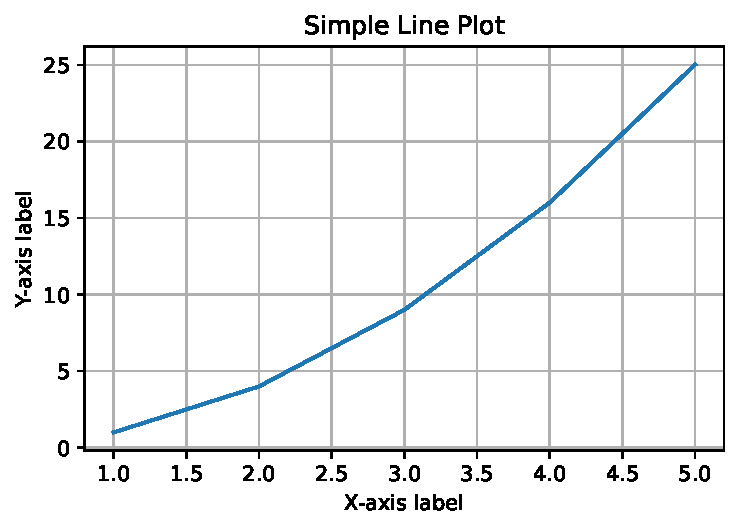
\includegraphics{15_Data_Vis_files/figure-pdf/cell-3-output-1.pdf}

}

\end{figure}

This example creates a simple line plot with labeled axes, a title, and
a grid. The method \texttt{plt.show()} is used to render the plot.

\hypertarget{types-of-plots-in-matplotlib}{%
\subsection{Types of Plots in
Matplotlib}\label{types-of-plots-in-matplotlib}}

Matplotlib supports a wide variety of plot types beyond simple line
graphs. Some of the most commonly used plot types include:

\begin{enumerate}
\def\labelenumi{\arabic{enumi}.}
\tightlist
\item
  \textbf{Scatter Plots}: Useful for exploring relationships between two
  variables.
\item
  \textbf{Bar Charts}: Ideal for comparing discrete categories.
\item
  \textbf{Histograms}: Commonly used to display the distribution of
  data.
\item
  \textbf{Pie Charts}: Used to show proportions of a whole.
\item
  \textbf{Box Plots}: Effective for visualizing the spread and outliers
  of data.
\end{enumerate}

\textbf{Example: Creating a Scatter Plot}

\begin{Shaded}
\begin{Highlighting}[]
\CommentTok{\# Data for scatter plot}
\NormalTok{x }\OperatorTok{=}\NormalTok{ [}\DecValTok{5}\NormalTok{, }\DecValTok{7}\NormalTok{, }\DecValTok{8}\NormalTok{, }\DecValTok{5}\NormalTok{, }\DecValTok{9}\NormalTok{, }\DecValTok{7}\NormalTok{]}
\NormalTok{y }\OperatorTok{=}\NormalTok{ [}\DecValTok{3}\NormalTok{, }\DecValTok{8}\NormalTok{, }\DecValTok{4}\NormalTok{, }\DecValTok{7}\NormalTok{, }\DecValTok{2}\NormalTok{, }\DecValTok{5}\NormalTok{]}

\CommentTok{\# Creating the scatter plot}
\NormalTok{plt.scatter(x, y, color}\OperatorTok{=}\StringTok{\textquotesingle{}blue\textquotesingle{}}\NormalTok{, marker}\OperatorTok{=}\StringTok{\textquotesingle{}\^{}\textquotesingle{}}\NormalTok{)}
\NormalTok{plt.xlabel(}\StringTok{\textquotesingle{}X{-}axis label\textquotesingle{}}\NormalTok{)}
\NormalTok{plt.ylabel(}\StringTok{\textquotesingle{}Y{-}axis label\textquotesingle{}}\NormalTok{)}
\NormalTok{plt.title(}\StringTok{\textquotesingle{}Scatter Plot Example\textquotesingle{}}\NormalTok{)}
\NormalTok{plt.show()}
\end{Highlighting}
\end{Shaded}

\begin{figure}[H]

{\centering 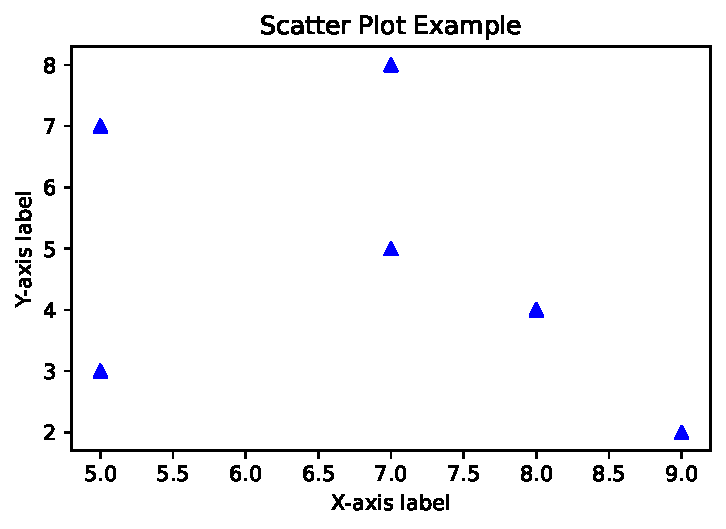
\includegraphics{15_Data_Vis_files/figure-pdf/cell-4-output-1.pdf}

}

\end{figure}

In this example, we use \texttt{plt.scatter()} to create a scatter plot,
where the color and marker style of the points can be easily customized.

\hypertarget{customizing-plots-in-matplotlib}{%
\subsection{Customizing Plots in
Matplotlib}\label{customizing-plots-in-matplotlib}}

Customization is one of Matplotlib's greatest strengths. You can modify
almost every aspect of a plot, including colors, line styles, markers,
axis scales, legends, and more. This flexibility allows you to create
publication-quality visualizations.

\textbf{Example: Customizing a Line Plot}

\begin{Shaded}
\begin{Highlighting}[]
\CommentTok{\# Customizing the line plot}
\NormalTok{plt.plot(x, y, color}\OperatorTok{=}\StringTok{\textquotesingle{}red\textquotesingle{}}\NormalTok{, linestyle}\OperatorTok{=}\StringTok{\textquotesingle{}{-}{-}\textquotesingle{}}\NormalTok{, linewidth}\OperatorTok{=}\DecValTok{2}\NormalTok{, marker}\OperatorTok{=}\StringTok{\textquotesingle{}o\textquotesingle{}}\NormalTok{, markersize}\OperatorTok{=}\DecValTok{8}\NormalTok{, markerfacecolor}\OperatorTok{=}\StringTok{\textquotesingle{}yellow\textquotesingle{}}\NormalTok{)}
\NormalTok{plt.xlabel(}\StringTok{\textquotesingle{}X{-}axis label\textquotesingle{}}\NormalTok{)}
\NormalTok{plt.ylabel(}\StringTok{\textquotesingle{}Y{-}axis label\textquotesingle{}}\NormalTok{)}
\NormalTok{plt.title(}\StringTok{\textquotesingle{}Customized Line Plot\textquotesingle{}}\NormalTok{)}
\NormalTok{plt.grid(}\VariableTok{True}\NormalTok{)}
\NormalTok{plt.show()}
\end{Highlighting}
\end{Shaded}

\begin{figure}[H]

{\centering 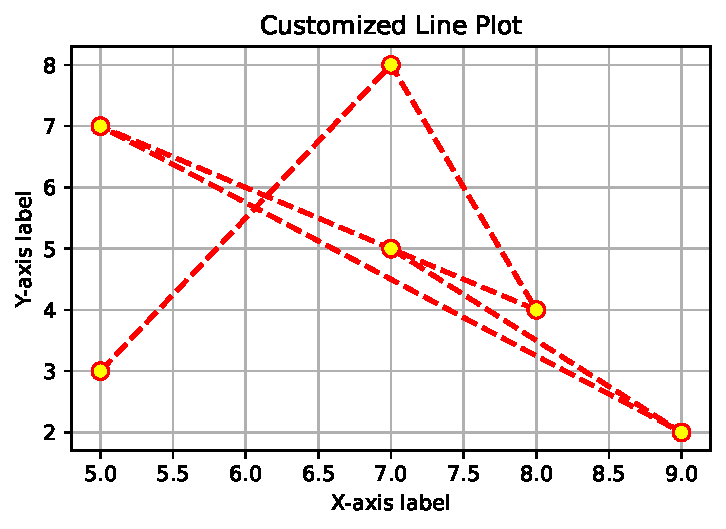
\includegraphics{15_Data_Vis_files/figure-pdf/cell-5-output-1.pdf}

}

\end{figure}

In this example, we modify the line style to be dashed (\texttt{-\/-}),
set the line color to red, increase the line width, and customize the
marker appearance with size and color adjustments.

\hypertarget{adding-annotations-and-legends}{%
\subsection{Adding Annotations and
Legends}\label{adding-annotations-and-legends}}

Annotations and legends can significantly enhance the interpretability
of your plots. Annotations allow you to highlight specific data points
or trends, while legends help distinguish different datasets in a
multi-line plot.

\textbf{Example: Adding a Legend and Annotations}

\begin{Shaded}
\begin{Highlighting}[]
\CommentTok{\# Data for multiple lines}
\NormalTok{x }\OperatorTok{=}\NormalTok{ [}\DecValTok{1}\NormalTok{, }\DecValTok{2}\NormalTok{, }\DecValTok{3}\NormalTok{, }\DecValTok{4}\NormalTok{, }\DecValTok{5}\NormalTok{]}
\NormalTok{y1 }\OperatorTok{=}\NormalTok{ [}\DecValTok{1}\NormalTok{, }\DecValTok{4}\NormalTok{, }\DecValTok{9}\NormalTok{, }\DecValTok{16}\NormalTok{, }\DecValTok{25}\NormalTok{]}
\NormalTok{y2 }\OperatorTok{=}\NormalTok{ [}\DecValTok{2}\NormalTok{, }\DecValTok{3}\NormalTok{, }\DecValTok{4}\NormalTok{, }\DecValTok{5}\NormalTok{, }\DecValTok{6}\NormalTok{]}

\CommentTok{\# Plotting multiple lines}
\NormalTok{plt.plot(x, y1, label}\OperatorTok{=}\StringTok{\textquotesingle{}Dataset 1\textquotesingle{}}\NormalTok{, color}\OperatorTok{=}\StringTok{\textquotesingle{}blue\textquotesingle{}}\NormalTok{)}
\NormalTok{plt.plot(x, y2, label}\OperatorTok{=}\StringTok{\textquotesingle{}Dataset 2\textquotesingle{}}\NormalTok{, color}\OperatorTok{=}\StringTok{\textquotesingle{}green\textquotesingle{}}\NormalTok{)}

\CommentTok{\# Adding an annotation}
\NormalTok{plt.annotate(}\StringTok{\textquotesingle{}Intersection\textquotesingle{}}\NormalTok{, xy}\OperatorTok{=}\NormalTok{(}\DecValTok{3}\NormalTok{, }\DecValTok{9}\NormalTok{), xytext}\OperatorTok{=}\NormalTok{(}\DecValTok{4}\NormalTok{, }\DecValTok{15}\NormalTok{),}
\NormalTok{             arrowprops}\OperatorTok{=}\BuiltInTok{dict}\NormalTok{(facecolor}\OperatorTok{=}\StringTok{\textquotesingle{}black\textquotesingle{}}\NormalTok{, shrink}\OperatorTok{=}\FloatTok{0.05}\NormalTok{))}

\CommentTok{\# Customizing plot}
\NormalTok{plt.xlabel(}\StringTok{\textquotesingle{}X{-}axis label\textquotesingle{}}\NormalTok{)}
\NormalTok{plt.ylabel(}\StringTok{\textquotesingle{}Y{-}axis label\textquotesingle{}}\NormalTok{)}
\NormalTok{plt.title(}\StringTok{\textquotesingle{}Annotated Plot with Legend\textquotesingle{}}\NormalTok{)}
\NormalTok{plt.legend(loc}\OperatorTok{=}\StringTok{\textquotesingle{}upper left\textquotesingle{}}\NormalTok{)}
\NormalTok{plt.grid(}\VariableTok{True}\NormalTok{)}
\NormalTok{plt.show()}
\end{Highlighting}
\end{Shaded}

\begin{figure}[H]

{\centering 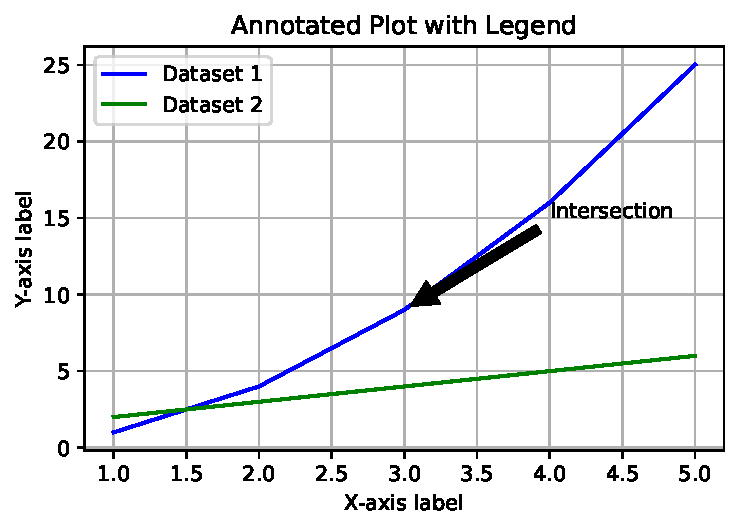
\includegraphics{15_Data_Vis_files/figure-pdf/cell-6-output-1.pdf}

}

\end{figure}

This example demonstrates how to use the \texttt{annotate()} function to
add a text label to a specific point on the plot, along with an arrow
pointing to that location. The \texttt{legend()} function is used to add
a legend that describes the different lines in the plot.

\hypertarget{working-with-subplots}{%
\subsection{Working with Subplots}\label{working-with-subplots}}

Subplots allow you to create multiple plots in a single figure, making
it easier to compare different visualizations side by side.

\textbf{Example: Creating Subplots}

\begin{Shaded}
\begin{Highlighting}[]
\CommentTok{\# Creating a figure with 2 rows and 1 column of subplots}
\NormalTok{fig, axs }\OperatorTok{=}\NormalTok{ plt.subplots(}\DecValTok{2}\NormalTok{, }\DecValTok{1}\NormalTok{, figsize}\OperatorTok{=}\NormalTok{(}\DecValTok{6}\NormalTok{, }\DecValTok{8}\NormalTok{))}

\CommentTok{\# First subplot}
\NormalTok{axs[}\DecValTok{0}\NormalTok{].plot(x, y1, color}\OperatorTok{=}\StringTok{\textquotesingle{}blue\textquotesingle{}}\NormalTok{)}
\NormalTok{axs[}\DecValTok{0}\NormalTok{].set\_title(}\StringTok{\textquotesingle{}Line Plot 1\textquotesingle{}}\NormalTok{)}
\NormalTok{axs[}\DecValTok{0}\NormalTok{].set\_xlabel(}\StringTok{\textquotesingle{}X{-}axis\textquotesingle{}}\NormalTok{)}
\NormalTok{axs[}\DecValTok{0}\NormalTok{].set\_ylabel(}\StringTok{\textquotesingle{}Y{-}axis\textquotesingle{}}\NormalTok{)}

\CommentTok{\# Second subplot}
\NormalTok{axs[}\DecValTok{1}\NormalTok{].scatter(x, y2, color}\OperatorTok{=}\StringTok{\textquotesingle{}green\textquotesingle{}}\NormalTok{)}
\NormalTok{axs[}\DecValTok{1}\NormalTok{].set\_title(}\StringTok{\textquotesingle{}Scatter Plot 2\textquotesingle{}}\NormalTok{)}
\NormalTok{axs[}\DecValTok{1}\NormalTok{].set\_xlabel(}\StringTok{\textquotesingle{}X{-}axis\textquotesingle{}}\NormalTok{)}
\NormalTok{axs[}\DecValTok{1}\NormalTok{].set\_ylabel(}\StringTok{\textquotesingle{}Y{-}axis\textquotesingle{}}\NormalTok{)}

\CommentTok{\# Display the plots}
\NormalTok{plt.tight\_layout()  }\CommentTok{\# Adjusts spacing between subplots}
\NormalTok{plt.show()}
\end{Highlighting}
\end{Shaded}

\begin{figure}[H]

{\centering 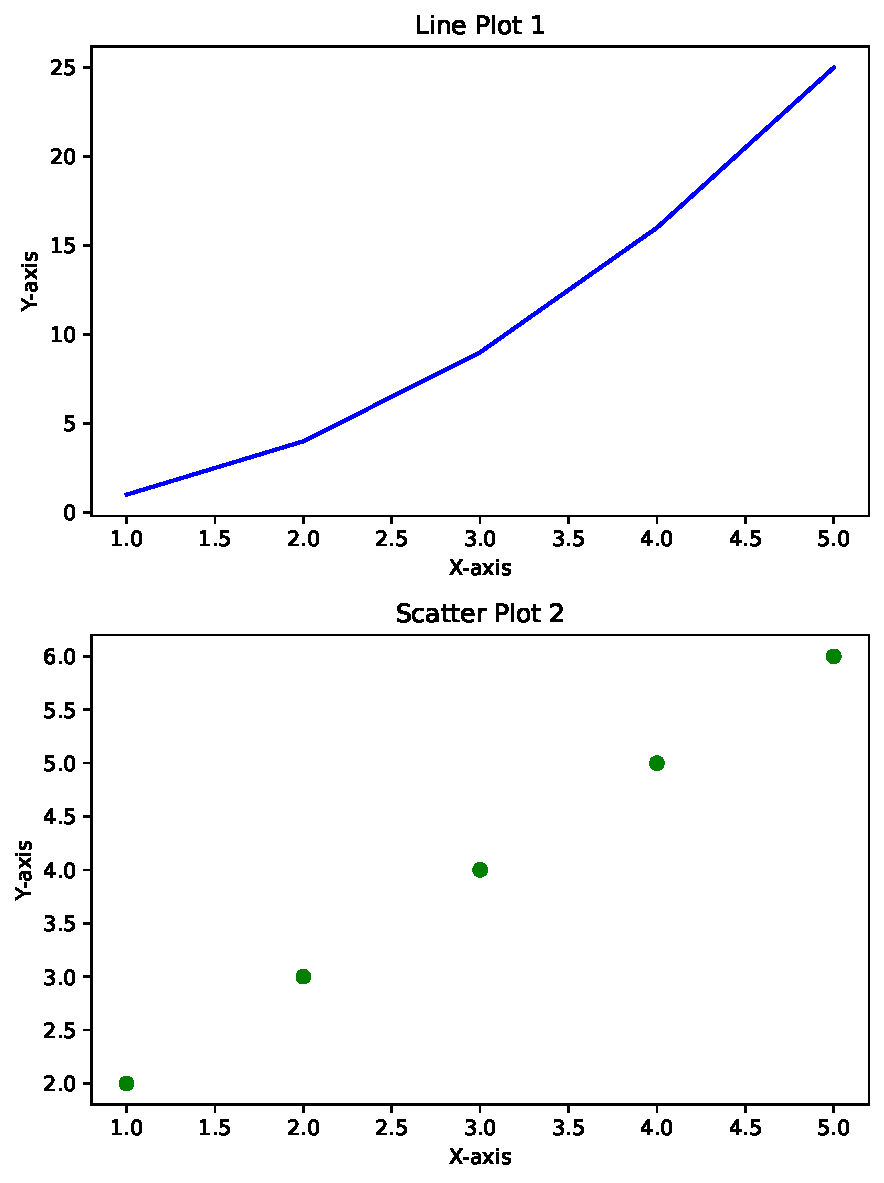
\includegraphics{15_Data_Vis_files/figure-pdf/cell-7-output-1.pdf}

}

\end{figure}

This example uses the \texttt{subplots()} function to create a figure
with two subplots arranged in a column. Each subplot is customized with
its own title, labels, and data.

\hypertarget{styling-and-themes-in-matplotlib}{%
\subsection{Styling and Themes in
Matplotlib}\label{styling-and-themes-in-matplotlib}}

Matplotlib offers several built-in styles that can be applied to your
plots to give them a consistent and visually appealing look. Styles can
be easily switched using the \texttt{plt.style.use()} function.

\textbf{Example: Using Different Styles}

\begin{Shaded}
\begin{Highlighting}[]
\CommentTok{\# Applying a style to the plot}
\NormalTok{plt.style.use(}\StringTok{\textquotesingle{}ggplot\textquotesingle{}}\NormalTok{)}

\CommentTok{\# Replotting the data with the new style}
\NormalTok{plt.plot(x, y1, color}\OperatorTok{=}\StringTok{\textquotesingle{}red\textquotesingle{}}\NormalTok{, linestyle}\OperatorTok{=}\StringTok{\textquotesingle{}{-}\textquotesingle{}}\NormalTok{, marker}\OperatorTok{=}\StringTok{\textquotesingle{}o\textquotesingle{}}\NormalTok{)}
\NormalTok{plt.title(}\StringTok{\textquotesingle{}Styled Plot with ggplot Theme\textquotesingle{}}\NormalTok{)}
\NormalTok{plt.xlabel(}\StringTok{\textquotesingle{}X{-}axis\textquotesingle{}}\NormalTok{)}
\NormalTok{plt.ylabel(}\StringTok{\textquotesingle{}Y{-}axis\textquotesingle{}}\NormalTok{)}
\NormalTok{plt.show()}

\CommentTok{\# Reset to the default style}
\NormalTok{plt.style.use(}\StringTok{\textquotesingle{}default\textquotesingle{}}\NormalTok{)}
\end{Highlighting}
\end{Shaded}

\begin{figure}[H]

{\centering 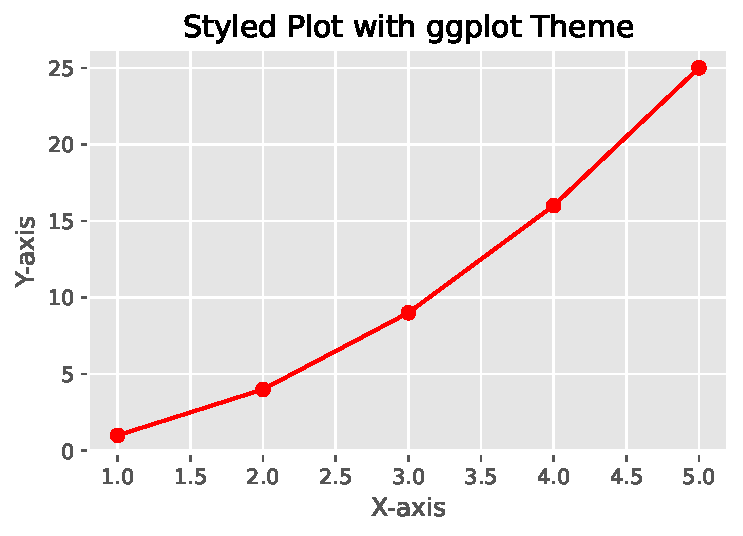
\includegraphics{15_Data_Vis_files/figure-pdf/cell-8-output-1.pdf}

}

\end{figure}

In this example, we apply the \texttt{ggplot} style to the plot, which
gives it a different color scheme and grid design inspired by the
aesthetics of the ggplot2 package in R.

\hypertarget{saving-plots-to-files}{%
\subsection{Saving Plots to Files}\label{saving-plots-to-files}}

Once you've created your visualizations, you might want to save them as
image files for use in presentations or publications.

\textbf{Example: Saving a Plot}

\begin{Shaded}
\begin{Highlighting}[]
\CommentTok{\# Saving the plot to a file}
\NormalTok{plt.plot(x, y1, color}\OperatorTok{=}\StringTok{\textquotesingle{}blue\textquotesingle{}}\NormalTok{, linestyle}\OperatorTok{=}\StringTok{\textquotesingle{}{-}{-}\textquotesingle{}}\NormalTok{)}
\NormalTok{plt.title(}\StringTok{\textquotesingle{}Plot to be Saved\textquotesingle{}}\NormalTok{)}
\NormalTok{plt.savefig(}\StringTok{\textquotesingle{}my\_plot.png\textquotesingle{}}\NormalTok{, dpi}\OperatorTok{=}\DecValTok{300}\NormalTok{, bbox\_inches}\OperatorTok{=}\StringTok{\textquotesingle{}tight\textquotesingle{}}\NormalTok{)}
\end{Highlighting}
\end{Shaded}

The \texttt{savefig()} function saves the plot as a PNG file with high
resolution (specified by \texttt{dpi=300}) and tight bounding boxes to
remove excess whitespace.

\hypertarget{common-pitfalls-and-best-practices}{%
\subsection{Common Pitfalls and Best
Practices}\label{common-pitfalls-and-best-practices}}

\begin{itemize}
\tightlist
\item
  \textbf{Aspect Ratio}: Always check the aspect ratio of your plots to
  ensure they are not distorted.
\item
  \textbf{Labels and Titles}: Make sure to label all axes and include a
  title to provide context to the visualization.
\item
  \textbf{Color Blindness}: Use color palettes that are accessible to
  those with color vision deficiencies.
\item
  \textbf{Legend Placement}: Place legends in a position that does not
  overlap with important data points.
\end{itemize}

Understanding how to leverage the power of Matplotlib will enable you to
create informative and professional-quality data visualizations,
enhancing your ability to communicate data-driven insights.

\hypertarget{introduction-to-seaborn}{%
\section{Introduction to Seaborn}\label{introduction-to-seaborn}}

Seaborn is a powerful Python visualization library built on top of
Matplotlib, designed specifically for creating informative and
attractive statistical graphics. It provides a high-level interface for
drawing a variety of statistical plots and integrates seamlessly with
data structures like Pandas DataFrames. Seaborn's design philosophy
emphasizes the importance of aesthetics, making it easy to generate
complex visualizations with concise code.

\hypertarget{getting-started-with-seaborn}{%
\subsection{Getting Started with
Seaborn}\label{getting-started-with-seaborn}}

To use Seaborn, you first need to import the library. If you haven't
already installed it, you can do so using the following command:

\begin{Shaded}
\begin{Highlighting}[]
\OperatorTok{!}\NormalTok{pip install seaborn}
\end{Highlighting}
\end{Shaded}

Once installed, import Seaborn into your Python environment:

\begin{Shaded}
\begin{Highlighting}[]
\ImportTok{import}\NormalTok{ seaborn }\ImportTok{as}\NormalTok{ sns}
\ImportTok{import}\NormalTok{ matplotlib.pyplot }\ImportTok{as}\NormalTok{ plt}
\end{Highlighting}
\end{Shaded}

\hypertarget{creating-basic-plots-with-seaborn}{%
\subsection{Creating Basic Plots with
Seaborn}\label{creating-basic-plots-with-seaborn}}

Seaborn simplifies the process of creating plots by offering specific
functions for different types of statistical visualizations. Some of the
most commonly used plot types include scatter plots, line plots,
histograms, and bar charts.

\textbf{Example: Creating a Scatter Plot}

\begin{Shaded}
\begin{Highlighting}[]
\CommentTok{\# Sample data}
\NormalTok{tips }\OperatorTok{=}\NormalTok{ sns.load\_dataset(}\StringTok{\textquotesingle{}tips\textquotesingle{}}\NormalTok{)}

\CommentTok{\# Creating a scatter plot}
\NormalTok{sns.scatterplot(x}\OperatorTok{=}\StringTok{\textquotesingle{}total\_bill\textquotesingle{}}\NormalTok{, y}\OperatorTok{=}\StringTok{\textquotesingle{}tip\textquotesingle{}}\NormalTok{, data}\OperatorTok{=}\NormalTok{tips)}
\NormalTok{plt.title(}\StringTok{\textquotesingle{}Scatter Plot of Total Bill vs. Tip\textquotesingle{}}\NormalTok{)}
\NormalTok{plt.xlabel(}\StringTok{\textquotesingle{}Total Bill\textquotesingle{}}\NormalTok{)}
\NormalTok{plt.ylabel(}\StringTok{\textquotesingle{}Tip\textquotesingle{}}\NormalTok{)}
\NormalTok{plt.show()}
\end{Highlighting}
\end{Shaded}

\begin{figure}[H]

{\centering 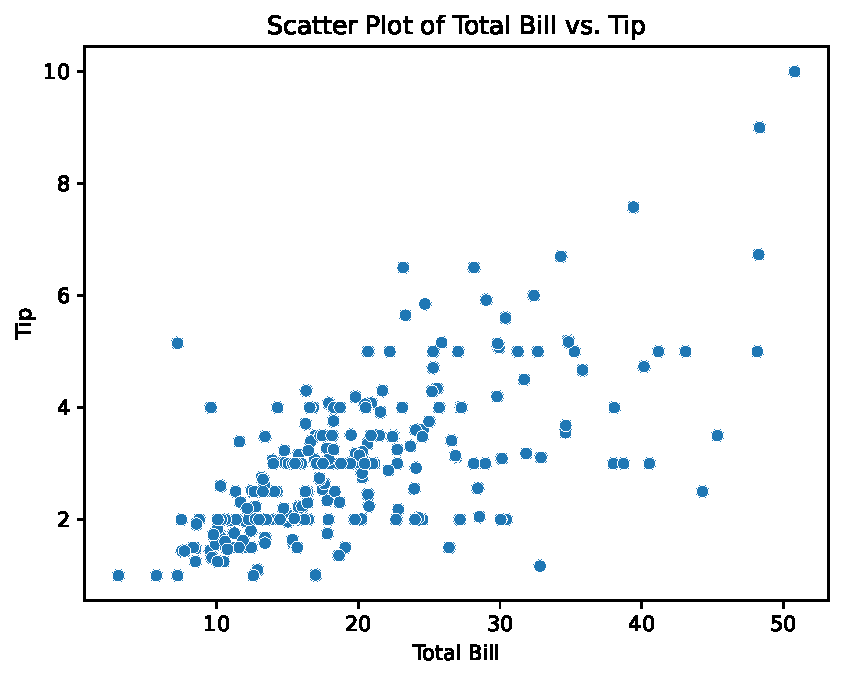
\includegraphics{15_Data_Vis_files/figure-pdf/cell-10-output-1.pdf}

}

\end{figure}

In this example, we use the \texttt{tips} dataset (which is built into
Seaborn) to create a scatter plot that shows the relationship between
the total bill and the tip amount.

\hypertarget{customizing-visualizations-with-seaborn}{%
\subsection{Customizing Visualizations with
Seaborn}\label{customizing-visualizations-with-seaborn}}

Seaborn allows extensive customization of plot aesthetics to make
visualizations more informative and appealing. You can easily modify
colors, markers, and styles.

\textbf{Example: Customizing a Scatter Plot}

\begin{Shaded}
\begin{Highlighting}[]
\CommentTok{\# Custom scatter plot with color and marker variations}
\NormalTok{sns.scatterplot(x}\OperatorTok{=}\StringTok{\textquotesingle{}total\_bill\textquotesingle{}}\NormalTok{, y}\OperatorTok{=}\StringTok{\textquotesingle{}tip\textquotesingle{}}\NormalTok{, hue}\OperatorTok{=}\StringTok{\textquotesingle{}sex\textquotesingle{}}\NormalTok{, style}\OperatorTok{=}\StringTok{\textquotesingle{}smoker\textquotesingle{}}\NormalTok{, size}\OperatorTok{=}\StringTok{\textquotesingle{}size\textquotesingle{}}\NormalTok{, data}\OperatorTok{=}\NormalTok{tips)}
\NormalTok{plt.title(}\StringTok{\textquotesingle{}Customized Scatter Plot of Total Bill vs. Tip\textquotesingle{}}\NormalTok{)}
\NormalTok{plt.xlabel(}\StringTok{\textquotesingle{}Total Bill\textquotesingle{}}\NormalTok{)}
\NormalTok{plt.ylabel(}\StringTok{\textquotesingle{}Tip\textquotesingle{}}\NormalTok{)}
\NormalTok{plt.show()}
\end{Highlighting}
\end{Shaded}

\begin{figure}[H]

{\centering 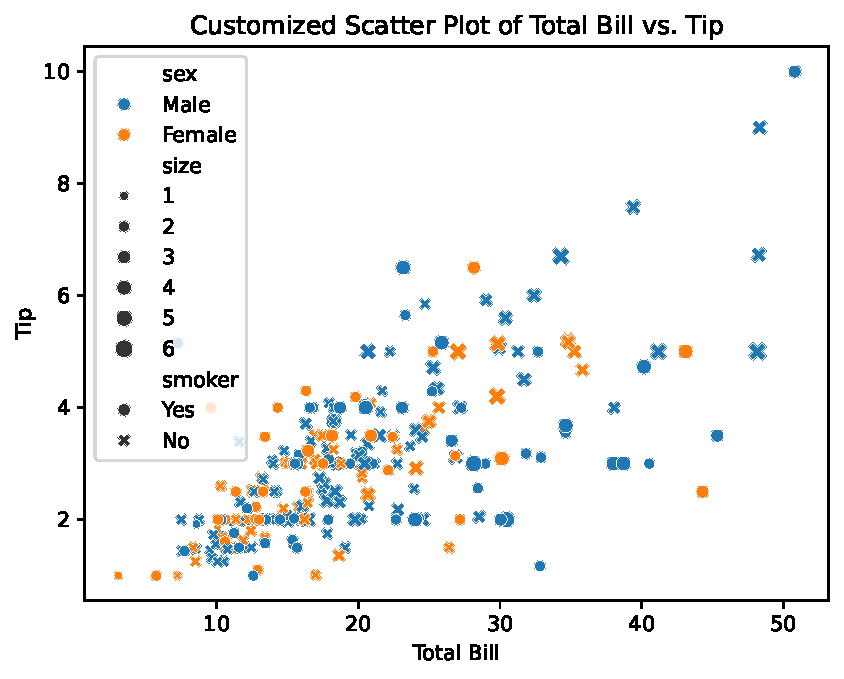
\includegraphics{15_Data_Vis_files/figure-pdf/cell-11-output-1.pdf}

}

\end{figure}

Here, the scatter plot is customized to differentiate data points based
on additional variables using color (\texttt{hue}), marker style
(\texttt{style}), and size (\texttt{size}). This makes it easier to
visualize relationships between multiple variables in a single plot.

\hypertarget{visualizing-distributions}{%
\subsection{Visualizing Distributions}\label{visualizing-distributions}}

Understanding the distribution of data is crucial in statistical
analysis. Seaborn offers several functions specifically for visualizing
distributions, such as histograms, KDE plots, and box plots.

\textbf{Example: Creating a Histogram and KDE Plot}

\begin{Shaded}
\begin{Highlighting}[]
\CommentTok{\# Histogram and KDE plot for total bill}
\NormalTok{sns.histplot(tips[}\StringTok{\textquotesingle{}total\_bill\textquotesingle{}}\NormalTok{], kde}\OperatorTok{=}\VariableTok{True}\NormalTok{, color}\OperatorTok{=}\StringTok{\textquotesingle{}blue\textquotesingle{}}\NormalTok{)}
\NormalTok{plt.title(}\StringTok{\textquotesingle{}Distribution of Total Bill with Histogram and KDE\textquotesingle{}}\NormalTok{)}
\NormalTok{plt.xlabel(}\StringTok{\textquotesingle{}Total Bill\textquotesingle{}}\NormalTok{)}
\NormalTok{plt.ylabel(}\StringTok{\textquotesingle{}Frequency\textquotesingle{}}\NormalTok{)}
\NormalTok{plt.show()}
\end{Highlighting}
\end{Shaded}

\begin{figure}[H]

{\centering 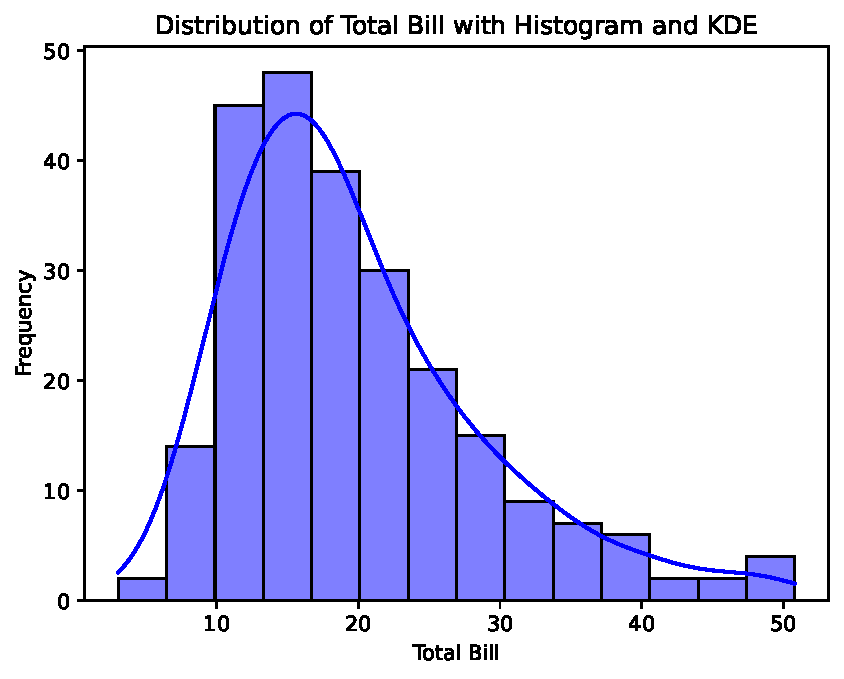
\includegraphics{15_Data_Vis_files/figure-pdf/cell-12-output-1.pdf}

}

\end{figure}

In this example, we create a histogram of the \texttt{total\_bill}
variable with an overlaid Kernel Density Estimate (KDE), which provides
a smoothed curve representing the distribution.

\hypertarget{creating-categorical-plots}{%
\subsection{Creating Categorical
Plots}\label{creating-categorical-plots}}

Seaborn excels in creating categorical plots that help analyze the
relationship between categorical data and numerical data. The most
common types include bar plots, box plots, and violin plots.

\textbf{Example: Bar Plot}

\begin{Shaded}
\begin{Highlighting}[]
\CommentTok{\# Bar plot showing the average tip amount by day}
\NormalTok{sns.barplot(x}\OperatorTok{=}\StringTok{\textquotesingle{}day\textquotesingle{}}\NormalTok{, y}\OperatorTok{=}\StringTok{\textquotesingle{}tip\textquotesingle{}}\NormalTok{, data}\OperatorTok{=}\NormalTok{tips, ci}\OperatorTok{=}\StringTok{\textquotesingle{}sd\textquotesingle{}}\NormalTok{, palette}\OperatorTok{=}\StringTok{\textquotesingle{}viridis\textquotesingle{}}\NormalTok{)}
\NormalTok{plt.title(}\StringTok{\textquotesingle{}Average Tip by Day\textquotesingle{}}\NormalTok{)}
\NormalTok{plt.xlabel(}\StringTok{\textquotesingle{}Day\textquotesingle{}}\NormalTok{)}
\NormalTok{plt.ylabel(}\StringTok{\textquotesingle{}Average Tip\textquotesingle{}}\NormalTok{)}
\NormalTok{plt.show()}
\end{Highlighting}
\end{Shaded}

\begin{verbatim}
C:\Users\Joshua_Patrick\AppData\Local\Temp\ipykernel_42632\690395935.py:2: FutureWarning: 

The `ci` parameter is deprecated. Use `errorbar='sd'` for the same effect.

  sns.barplot(x='day', y='tip', data=tips, ci='sd', palette='viridis')
C:\Users\Joshua_Patrick\AppData\Local\Temp\ipykernel_42632\690395935.py:2: FutureWarning: 

Passing `palette` without assigning `hue` is deprecated and will be removed in v0.14.0. Assign the `x` variable to `hue` and set `legend=False` for the same effect.

  sns.barplot(x='day', y='tip', data=tips, ci='sd', palette='viridis')
\end{verbatim}

\begin{figure}[H]

{\centering 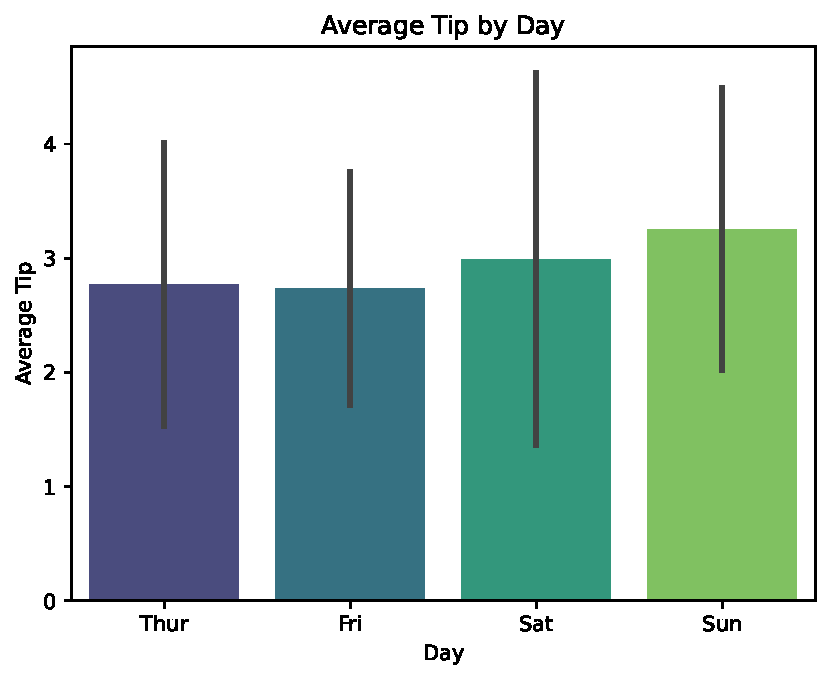
\includegraphics{15_Data_Vis_files/figure-pdf/cell-13-output-2.pdf}

}

\end{figure}

This bar plot displays the average tip amount for each day of the week,
using error bars to indicate the standard deviation. Seaborn's color
palettes, like \texttt{viridis}, enhance the plot's visual appeal.

\textbf{Example: Box Plot}

\begin{Shaded}
\begin{Highlighting}[]
\CommentTok{\# Box plot showing the distribution of total bill by day}
\NormalTok{sns.boxplot(x}\OperatorTok{=}\StringTok{\textquotesingle{}day\textquotesingle{}}\NormalTok{, y}\OperatorTok{=}\StringTok{\textquotesingle{}total\_bill\textquotesingle{}}\NormalTok{, hue}\OperatorTok{=}\StringTok{\textquotesingle{}smoker\textquotesingle{}}\NormalTok{, data}\OperatorTok{=}\NormalTok{tips, palette}\OperatorTok{=}\StringTok{\textquotesingle{}Set2\textquotesingle{}}\NormalTok{)}
\NormalTok{plt.title(}\StringTok{\textquotesingle{}Box Plot of Total Bill by Day\textquotesingle{}}\NormalTok{)}
\NormalTok{plt.xlabel(}\StringTok{\textquotesingle{}Day\textquotesingle{}}\NormalTok{)}
\NormalTok{plt.ylabel(}\StringTok{\textquotesingle{}Total Bill\textquotesingle{}}\NormalTok{)}
\NormalTok{plt.show()}
\end{Highlighting}
\end{Shaded}

\begin{figure}[H]

{\centering 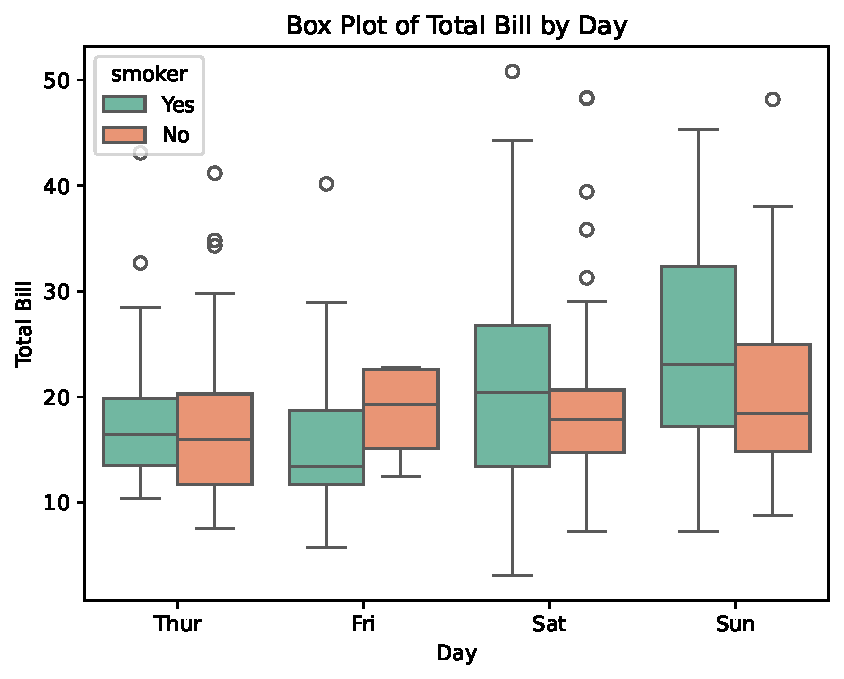
\includegraphics{15_Data_Vis_files/figure-pdf/cell-14-output-1.pdf}

}

\end{figure}

The box plot provides insights into the distribution of the
\texttt{total\_bill} by day, highlighting the median, interquartile
range (IQR), and potential outliers. The \texttt{hue} parameter adds
another layer to the plot, differentiating between smokers and
non-smokers.

\hypertarget{pair-plots-for-multivariate-analysis}{%
\subsection{Pair Plots for Multivariate
Analysis}\label{pair-plots-for-multivariate-analysis}}

Pair plots are useful for visualizing relationships between multiple
variables at once. They create a grid of scatter plots for each pair of
variables and display histograms for individual variable distributions.

\textbf{Example: Pair Plot}

\begin{Shaded}
\begin{Highlighting}[]
\CommentTok{\# Creating a pair plot of the tips dataset}
\NormalTok{sns.pairplot(tips, hue}\OperatorTok{=}\StringTok{\textquotesingle{}sex\textquotesingle{}}\NormalTok{, palette}\OperatorTok{=}\StringTok{\textquotesingle{}coolwarm\textquotesingle{}}\NormalTok{)}
\NormalTok{plt.suptitle(}\StringTok{\textquotesingle{}Pair Plot of the Tips Dataset\textquotesingle{}}\NormalTok{, y}\OperatorTok{=}\FloatTok{1.02}\NormalTok{)}
\NormalTok{plt.show()}
\end{Highlighting}
\end{Shaded}

\begin{figure}[H]

{\centering 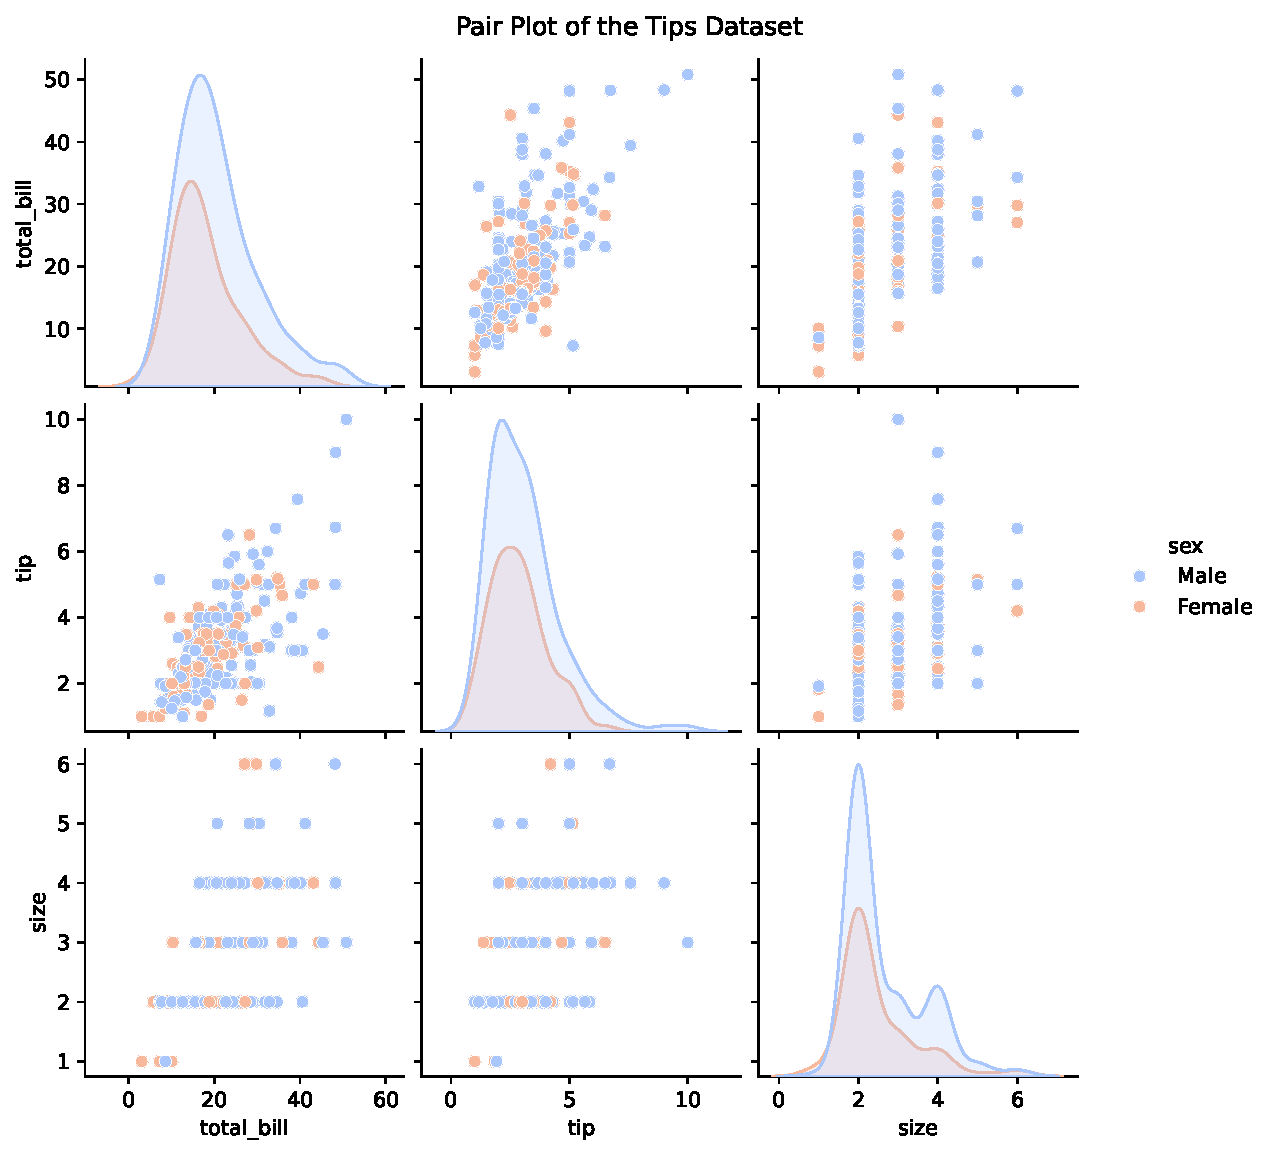
\includegraphics{15_Data_Vis_files/figure-pdf/cell-15-output-1.pdf}

}

\end{figure}

In this example, the pair plot provides a comprehensive view of pairwise
relationships between all numerical variables in the dataset, with
color-coded distinctions based on the \texttt{sex} variable.

\hypertarget{heatmaps-for-correlation-analysis}{%
\subsection{Heatmaps for Correlation
Analysis}\label{heatmaps-for-correlation-analysis}}

Heatmaps are an effective way to visualize the correlation matrix of
numerical data, showing how strongly pairs of variables are related.

\textbf{Example: Creating a Heatmap}

\begin{Shaded}
\begin{Highlighting}[]
\CommentTok{\# Correlation heatmap for the tips dataset}
\NormalTok{corr }\OperatorTok{=}\NormalTok{ tips.corr(numeric\_only }\OperatorTok{=} \VariableTok{True}\NormalTok{)}
\NormalTok{sns.heatmap(corr, annot}\OperatorTok{=}\VariableTok{True}\NormalTok{, cmap}\OperatorTok{=}\StringTok{\textquotesingle{}coolwarm\textquotesingle{}}\NormalTok{, linewidths}\OperatorTok{=}\FloatTok{0.5}\NormalTok{)}
\NormalTok{plt.title(}\StringTok{\textquotesingle{}Correlation Heatmap of Tips Dataset\textquotesingle{}}\NormalTok{)}
\NormalTok{plt.show()}
\end{Highlighting}
\end{Shaded}

\begin{figure}[H]

{\centering 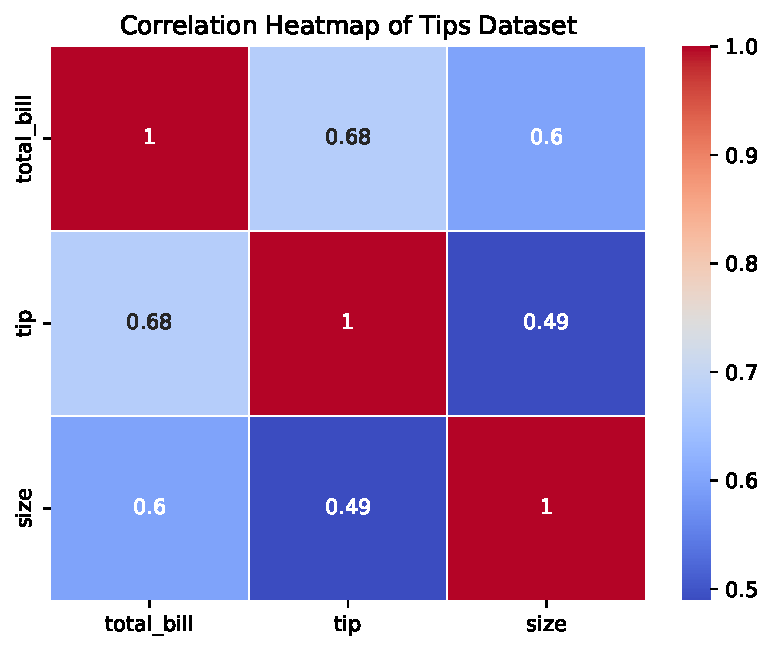
\includegraphics{15_Data_Vis_files/figure-pdf/cell-16-output-1.pdf}

}

\end{figure}

The heatmap in this example displays the correlation coefficients
between variables in the \texttt{tips} dataset, with color intensity
indicating the strength of the correlation. The \texttt{annot=True}
parameter ensures that the correlation values are displayed on the
heatmap.

\hypertarget{customizing-seaborn-themes}{%
\subsection{Customizing Seaborn
Themes}\label{customizing-seaborn-themes}}

Seaborn comes with several built-in themes to enhance the appearance of
plots, making it easy to change the overall look with minimal code.

\textbf{Example: Applying a Different Theme}

\begin{Shaded}
\begin{Highlighting}[]
\CommentTok{\# Set a Seaborn style for all plots}
\NormalTok{sns.set\_style(}\StringTok{\textquotesingle{}whitegrid\textquotesingle{}}\NormalTok{)}

\CommentTok{\# Creating a box plot with the new style}
\NormalTok{sns.boxplot(x}\OperatorTok{=}\StringTok{\textquotesingle{}day\textquotesingle{}}\NormalTok{, y}\OperatorTok{=}\StringTok{\textquotesingle{}total\_bill\textquotesingle{}}\NormalTok{, data}\OperatorTok{=}\NormalTok{tips, palette}\OperatorTok{=}\StringTok{\textquotesingle{}pastel\textquotesingle{}}\NormalTok{)}
\NormalTok{plt.title(}\StringTok{\textquotesingle{}Box Plot with Whitegrid Theme\textquotesingle{}}\NormalTok{)}
\NormalTok{plt.xlabel(}\StringTok{\textquotesingle{}Day\textquotesingle{}}\NormalTok{)}
\NormalTok{plt.ylabel(}\StringTok{\textquotesingle{}Total Bill\textquotesingle{}}\NormalTok{)}
\NormalTok{plt.show()}
\end{Highlighting}
\end{Shaded}

\begin{verbatim}
C:\Users\Joshua_Patrick\AppData\Local\Temp\ipykernel_42632\3431770401.py:5: FutureWarning: 

Passing `palette` without assigning `hue` is deprecated and will be removed in v0.14.0. Assign the `x` variable to `hue` and set `legend=False` for the same effect.

  sns.boxplot(x='day', y='total_bill', data=tips, palette='pastel')
\end{verbatim}

\begin{figure}[H]

{\centering 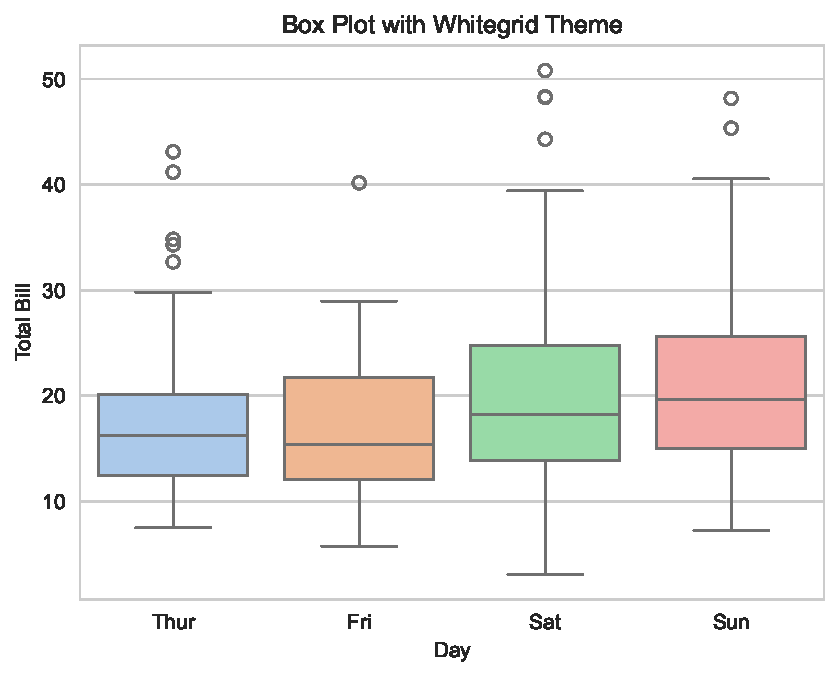
\includegraphics{15_Data_Vis_files/figure-pdf/cell-17-output-2.pdf}

}

\end{figure}

In this example, the \texttt{whitegrid} style adds grid lines to the
plot background, which can help in analyzing data points more
effectively.

\hypertarget{combining-seaborn-with-matplotlib}{%
\subsection{Combining Seaborn with
Matplotlib}\label{combining-seaborn-with-matplotlib}}

Although Seaborn provides a high-level interface for creating plots, it
is often beneficial to use Matplotlib functions for further
customization.

\textbf{Example: Combining Seaborn and Matplotlib for Plot
Customization}

\begin{Shaded}
\begin{Highlighting}[]
\CommentTok{\# Creating a violin plot with Seaborn}
\NormalTok{sns.violinplot(x}\OperatorTok{=}\StringTok{\textquotesingle{}day\textquotesingle{}}\NormalTok{, y}\OperatorTok{=}\StringTok{\textquotesingle{}total\_bill\textquotesingle{}}\NormalTok{, data}\OperatorTok{=}\NormalTok{tips, inner}\OperatorTok{=}\StringTok{\textquotesingle{}quartile\textquotesingle{}}\NormalTok{, palette}\OperatorTok{=}\StringTok{\textquotesingle{}Set3\textquotesingle{}}\NormalTok{)}

\CommentTok{\# Customizing with Matplotlib}
\NormalTok{plt.axhline(y}\OperatorTok{=}\DecValTok{20}\NormalTok{, color}\OperatorTok{=}\StringTok{\textquotesingle{}red\textquotesingle{}}\NormalTok{, linestyle}\OperatorTok{=}\StringTok{\textquotesingle{}{-}{-}\textquotesingle{}}\NormalTok{)  }\CommentTok{\# Add a reference line}
\NormalTok{plt.title(}\StringTok{\textquotesingle{}Violin Plot with Custom Reference Line\textquotesingle{}}\NormalTok{)}
\NormalTok{plt.xlabel(}\StringTok{\textquotesingle{}Day\textquotesingle{}}\NormalTok{)}
\NormalTok{plt.ylabel(}\StringTok{\textquotesingle{}Total Bill\textquotesingle{}}\NormalTok{)}
\NormalTok{plt.show()}
\end{Highlighting}
\end{Shaded}

\begin{verbatim}
C:\Users\Joshua_Patrick\AppData\Local\Temp\ipykernel_42632\122318432.py:2: FutureWarning: 

Passing `palette` without assigning `hue` is deprecated and will be removed in v0.14.0. Assign the `x` variable to `hue` and set `legend=False` for the same effect.

  sns.violinplot(x='day', y='total_bill', data=tips, inner='quartile', palette='Set3')
\end{verbatim}

\begin{figure}[H]

{\centering 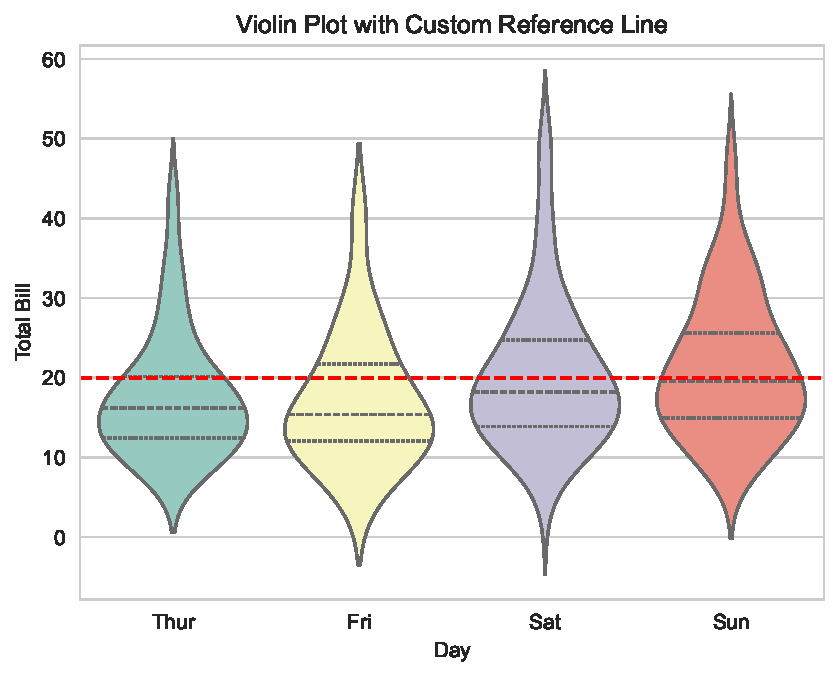
\includegraphics{15_Data_Vis_files/figure-pdf/cell-18-output-2.pdf}

}

\end{figure}

In this example, a Seaborn violin plot is enhanced with a Matplotlib
horizontal line, illustrating the synergy between the two libraries for
creating complex visualizations.

\hypertarget{advantages-of-using-seaborn}{%
\subsection{Advantages of Using
Seaborn}\label{advantages-of-using-seaborn}}

\begin{itemize}
\tightlist
\item
  \textbf{Simplified Syntax}: Seaborn's API is intuitive and reduces the
  code complexity for creating statistical graphics.
\item
  \textbf{Built-in Themes}: It offers aesthetically pleasing color
  palettes and themes that enhance the visual appeal.
\item
  \textbf{Integration with Pandas}: Seamlessly works with Pandas
  DataFrames, making data manipulation and visualization
  straightforward.
\item
  \textbf{Statistical Visualization}: Designed specifically for
  statistical plotting, providing functions that directly interpret and
  visualize statistical relationships.
\end{itemize}

\hypertarget{limitations-and-considerations}{%
\subsection{Limitations and
Considerations}\label{limitations-and-considerations}}

\begin{itemize}
\tightlist
\item
  \textbf{Customization Limitations}: Although Seaborn is powerful,
  certain highly specific customizations may require falling back on
  Matplotlib.
\item
  \textbf{Learning Curve}: Requires familiarity with data structures
  like DataFrames and understanding of statistical concepts for full
  utilization.
\end{itemize}

\hypertarget{introduction-to-ggplot-plotnine}{%
\section{Introduction to ggplot
(plotnine)}\label{introduction-to-ggplot-plotnine}}

The \texttt{ggplot} library in Python, made accessible through the
\texttt{plotnine} package, is inspired by the grammar of graphics
principles introduced by Leland Wilkinson. This approach allows data
visualizations to be built by combining independent layers, where each
layer adds a new element to the plot. This methodology enables the
creation of highly customizable and aesthetically pleasing plots with a
structured syntax that emphasizes clarity and reproducibility.

\hypertarget{the-grammar-of-graphics}{%
\subsection{The Grammar of Graphics}\label{the-grammar-of-graphics}}

The grammar of graphics is a theoretical framework that breaks down the
process of constructing data visualizations into independent components:

\begin{itemize}
\tightlist
\item
  \textbf{Data}: The dataset being visualized.
\item
  \textbf{Aesthetics (aes)}: The mapping of data variables to visual
  properties, such as position, color, and size.
\item
  \textbf{Geometries (geoms)}: The visual elements that represent data
  points, such as lines, bars, points, or histograms.
\item
  \textbf{Facets}: The ability to split data into subplots for
  comparison.
\item
  \textbf{Statistics}: Transformation or summary of data to highlight
  patterns.
\item
  \textbf{Scales}: Controls the mapping between data values and their
  visual representation.
\item
  \textbf{Coordinate systems}: Defines how data points are placed in a
  plot.
\end{itemize}

Understanding this layered approach helps in constructing meaningful and
well-organized visualizations.

\hypertarget{creating-a-basic-plot-with-ggplot}{%
\subsection{Creating a Basic Plot with
ggplot}\label{creating-a-basic-plot-with-ggplot}}

To use \texttt{ggplot} in Python, you will need to install the
\texttt{plotnine} package if you haven't already:

\begin{Shaded}
\begin{Highlighting}[]
\OperatorTok{!}\NormalTok{pip install plotnine}
\end{Highlighting}
\end{Shaded}

Now, let's begin by creating a basic line plot using \texttt{plotnine}.
We will use a simple dataset to demonstrate how to create a
visualization using the \texttt{ggplot} syntax.

\begin{Shaded}
\begin{Highlighting}[]
\ImportTok{import}\NormalTok{ pandas }\ImportTok{as}\NormalTok{ pd}
\ImportTok{from}\NormalTok{ plotnine }\ImportTok{import}\NormalTok{ ggplot, aes, geom\_line, ggtitle}

\CommentTok{\# Creating a dataset}
\NormalTok{data }\OperatorTok{=}\NormalTok{ pd.DataFrame(\{}
    \StringTok{\textquotesingle{}x\textquotesingle{}}\NormalTok{: [}\DecValTok{1}\NormalTok{, }\DecValTok{2}\NormalTok{, }\DecValTok{3}\NormalTok{, }\DecValTok{4}\NormalTok{, }\DecValTok{5}\NormalTok{],}
    \StringTok{\textquotesingle{}y\textquotesingle{}}\NormalTok{: [}\DecValTok{1}\NormalTok{, }\DecValTok{4}\NormalTok{, }\DecValTok{9}\NormalTok{, }\DecValTok{16}\NormalTok{, }\DecValTok{25}\NormalTok{]}
\NormalTok{\})}

\CommentTok{\# Creating a basic line plot}
\NormalTok{(ggplot(data, aes(x}\OperatorTok{=}\StringTok{\textquotesingle{}x\textquotesingle{}}\NormalTok{, y}\OperatorTok{=}\StringTok{\textquotesingle{}y\textquotesingle{}}\NormalTok{)) }\OperatorTok{+}
\NormalTok{ geom\_line() }\OperatorTok{+}
\NormalTok{ ggtitle(}\StringTok{\textquotesingle{}Basic Line Plot with ggplot\textquotesingle{}}\NormalTok{))}
\end{Highlighting}
\end{Shaded}

\begin{figure}[H]

{\centering 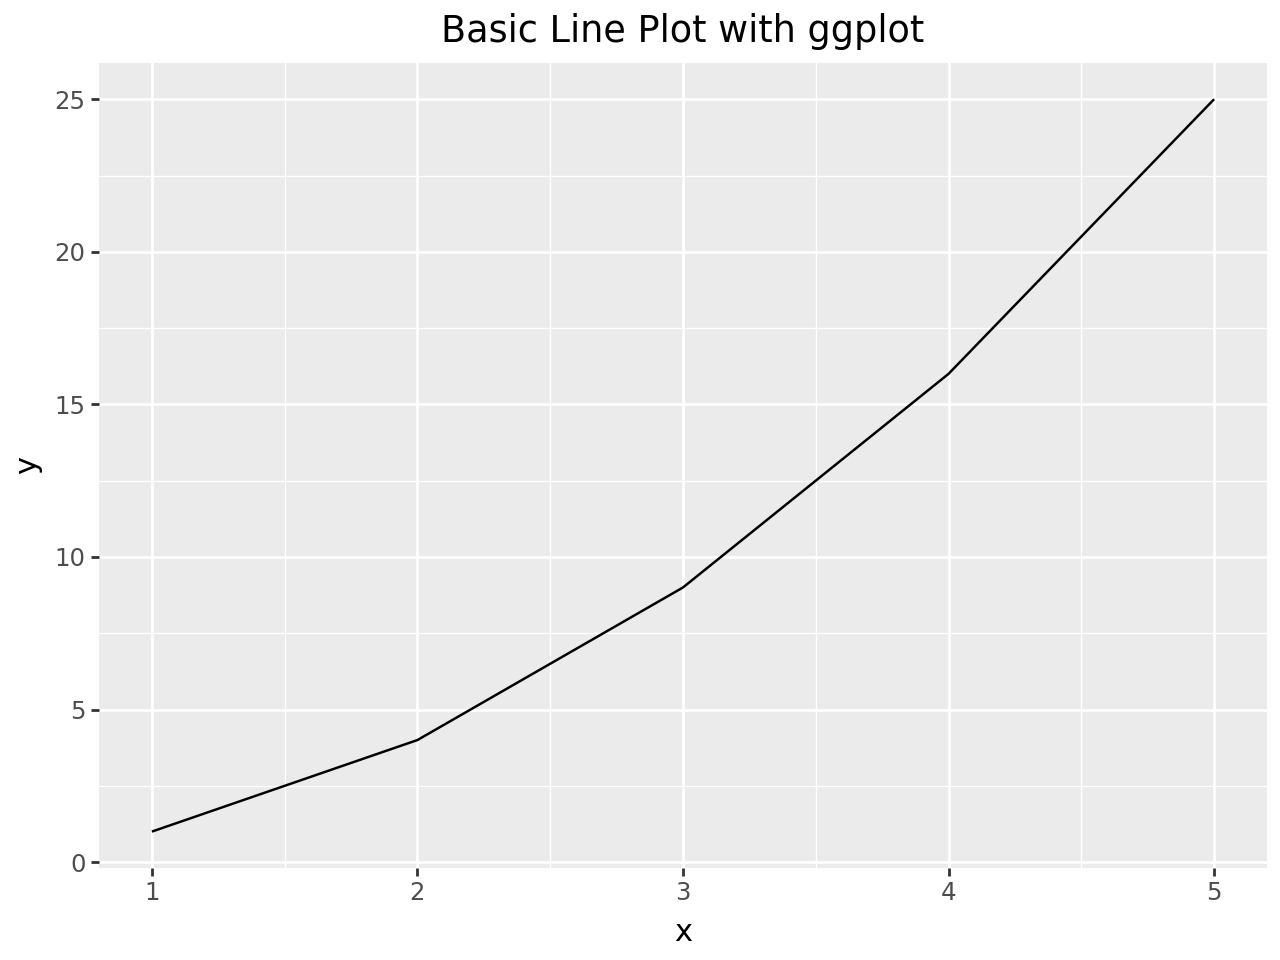
\includegraphics{15_Data_Vis_files/figure-pdf/cell-19-output-1.png}

}

\end{figure}

In this example, we define the dataset and specify the aesthetics using
\texttt{aes()}, which maps the \texttt{x} and \texttt{y} variables to
the axes of the plot. The \texttt{geom\_line()} function adds a line
graph layer to the plot. The title is set using \texttt{ggtitle()}.

\hypertarget{enhancing-visualizations-with-layers}{%
\subsection{Enhancing Visualizations with
Layers}\label{enhancing-visualizations-with-layers}}

One of the strengths of \texttt{ggplot} is the ability to add multiple
layers to a plot, allowing you to build more informative visualizations.

\textbf{Example: Adding Points to a Line Plot}

\begin{Shaded}
\begin{Highlighting}[]
\ImportTok{from}\NormalTok{ plotnine }\ImportTok{import}\NormalTok{ geom\_point, xlab, ylab}

\CommentTok{\# Adding a layer of points to the line plot}
\NormalTok{(ggplot(data, aes(x}\OperatorTok{=}\StringTok{\textquotesingle{}x\textquotesingle{}}\NormalTok{, y}\OperatorTok{=}\StringTok{\textquotesingle{}y\textquotesingle{}}\NormalTok{)) }\OperatorTok{+}
\NormalTok{ geom\_line(color}\OperatorTok{=}\StringTok{\textquotesingle{}blue\textquotesingle{}}\NormalTok{) }\OperatorTok{+}
\NormalTok{ geom\_point(color}\OperatorTok{=}\StringTok{\textquotesingle{}red\textquotesingle{}}\NormalTok{, size}\OperatorTok{=}\DecValTok{3}\NormalTok{) }\OperatorTok{+}
\NormalTok{ ggtitle(}\StringTok{\textquotesingle{}Enhanced Line Plot with Points\textquotesingle{}}\NormalTok{) }\OperatorTok{+}
\NormalTok{ xlab(}\StringTok{\textquotesingle{}X{-}axis\textquotesingle{}}\NormalTok{) }\OperatorTok{+}
\NormalTok{ ylab(}\StringTok{\textquotesingle{}Y{-}axis\textquotesingle{}}\NormalTok{))}
\end{Highlighting}
\end{Shaded}

\begin{figure}[H]

{\centering 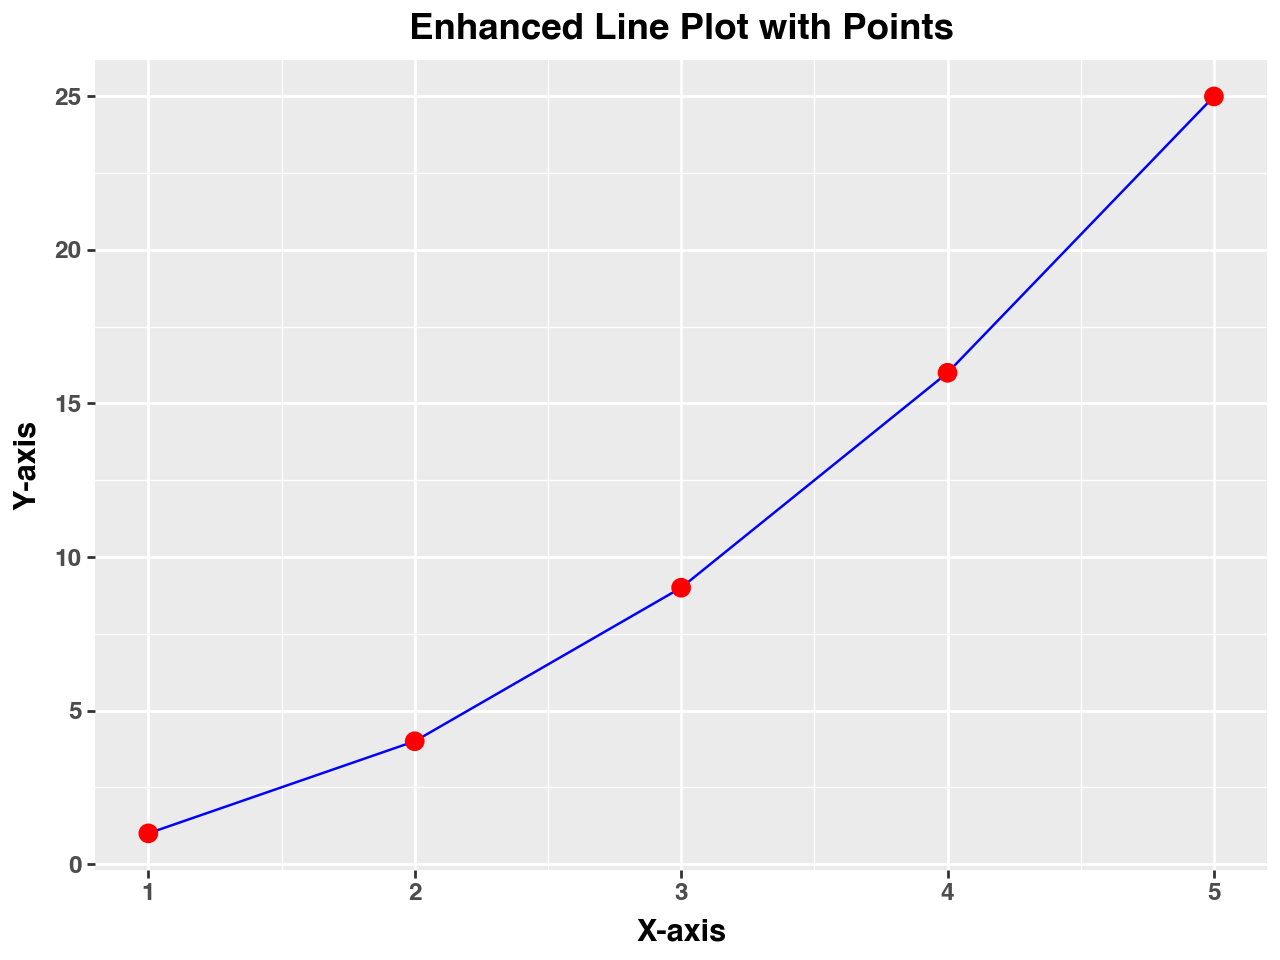
\includegraphics{15_Data_Vis_files/figure-pdf/cell-20-output-1.png}

}

\end{figure}

Here, we use the \texttt{geom\_point()} function to overlay points on
the existing line plot. This combination helps highlight individual data
points while still showing the overall trend.

\hypertarget{common-plot-types-in-ggplot}{%
\subsection{Common Plot Types in
ggplot}\label{common-plot-types-in-ggplot}}

\texttt{ggplot} supports a wide variety of plot types, each suited for
different types of data analysis:

\begin{enumerate}
\def\labelenumi{\arabic{enumi}.}
\tightlist
\item
  \textbf{Scatter Plots}: Used to visualize relationships between two
  continuous variables.
\item
  \textbf{Bar Charts}: Ideal for comparing categorical data.
\item
  \textbf{Histograms}: Useful for visualizing the distribution of a
  single variable.
\item
  \textbf{Box Plots}: Helps to visualize the spread, central tendency,
  and outliers in data.
\end{enumerate}

\textbf{Example: Creating a Scatter Plot}

\begin{Shaded}
\begin{Highlighting}[]
\CommentTok{\# Creating a dataset for the scatter plot}
\NormalTok{scatter\_data }\OperatorTok{=}\NormalTok{ pd.DataFrame(\{}
    \StringTok{\textquotesingle{}x\textquotesingle{}}\NormalTok{: [}\DecValTok{5}\NormalTok{, }\DecValTok{7}\NormalTok{, }\DecValTok{8}\NormalTok{, }\DecValTok{5}\NormalTok{, }\DecValTok{9}\NormalTok{, }\DecValTok{7}\NormalTok{],}
    \StringTok{\textquotesingle{}y\textquotesingle{}}\NormalTok{: [}\DecValTok{3}\NormalTok{, }\DecValTok{8}\NormalTok{, }\DecValTok{4}\NormalTok{, }\DecValTok{7}\NormalTok{, }\DecValTok{2}\NormalTok{, }\DecValTok{5}\NormalTok{]}
\NormalTok{\})}

\CommentTok{\# Scatter plot with ggplot}
\NormalTok{(ggplot(scatter\_data, aes(x}\OperatorTok{=}\StringTok{\textquotesingle{}x\textquotesingle{}}\NormalTok{, y}\OperatorTok{=}\StringTok{\textquotesingle{}y\textquotesingle{}}\NormalTok{)) }\OperatorTok{+}
\NormalTok{ geom\_point(color}\OperatorTok{=}\StringTok{\textquotesingle{}green\textquotesingle{}}\NormalTok{, size}\OperatorTok{=}\DecValTok{4}\NormalTok{) }\OperatorTok{+}
\NormalTok{ ggtitle(}\StringTok{\textquotesingle{}Scatter Plot Example\textquotesingle{}}\NormalTok{) }\OperatorTok{+}
\NormalTok{ xlab(}\StringTok{\textquotesingle{}X{-}axis Label\textquotesingle{}}\NormalTok{) }\OperatorTok{+}
\NormalTok{ ylab(}\StringTok{\textquotesingle{}Y{-}axis Label\textquotesingle{}}\NormalTok{))}
\end{Highlighting}
\end{Shaded}

\begin{figure}[H]

{\centering 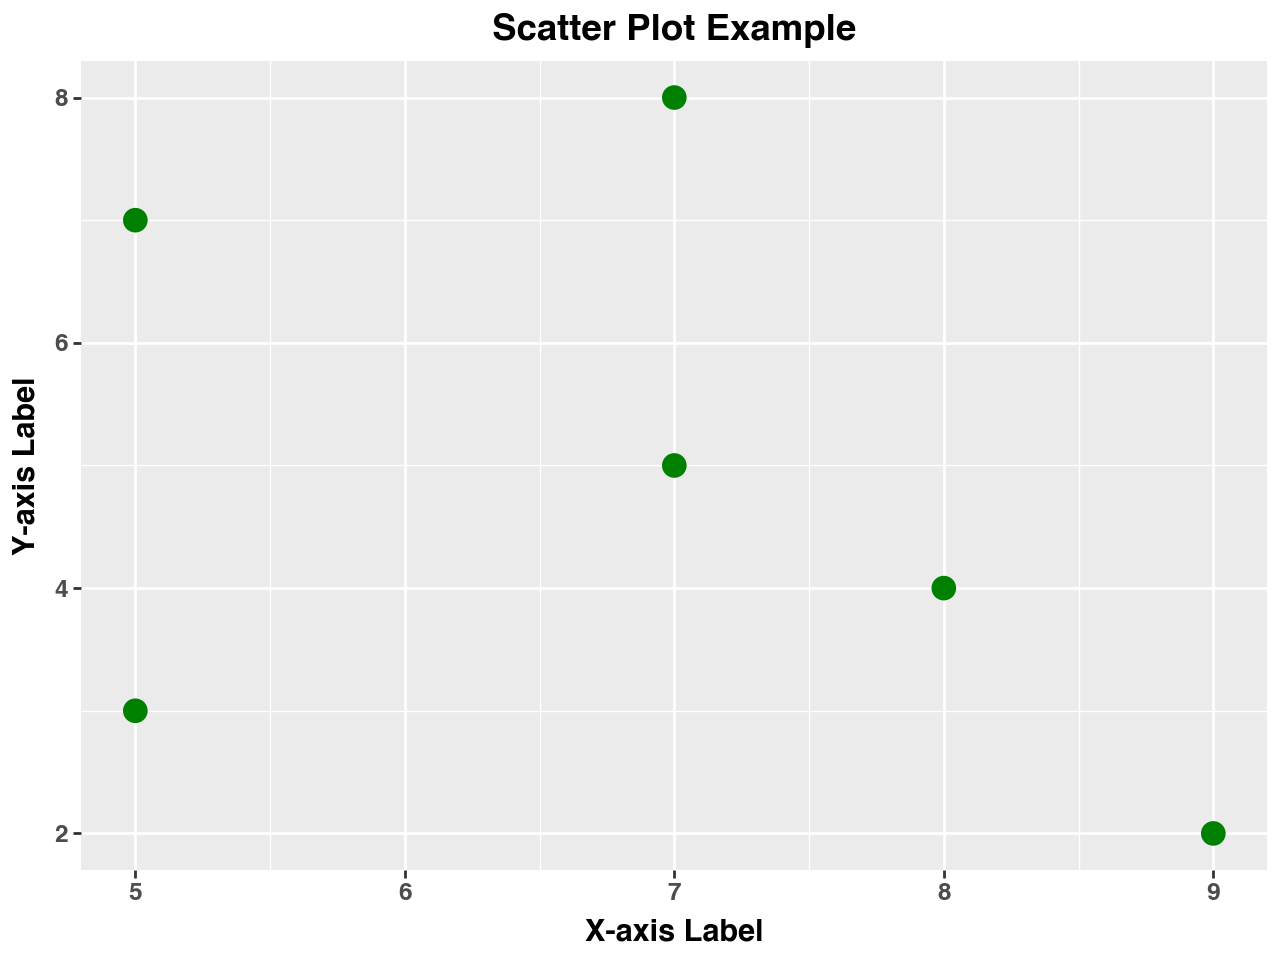
\includegraphics{15_Data_Vis_files/figure-pdf/cell-21-output-1.png}

}

\end{figure}

In this example, the scatter plot is created using
\texttt{geom\_point()}, with customizations for point color and size.

\hypertarget{faceting-for-multi-plot-layouts}{%
\subsection{Faceting for Multi-Plot
Layouts}\label{faceting-for-multi-plot-layouts}}

Faceting in \texttt{ggplot} allows you to create multiple subplots
within a single plot, enabling easy comparison of different subsets of
the data. Faceting can be done by rows, columns, or both.

\textbf{Example: Faceting with a Categorical Variable}

\begin{Shaded}
\begin{Highlighting}[]
\ImportTok{from}\NormalTok{ plotnine }\ImportTok{import}\NormalTok{ facet\_wrap}

\CommentTok{\# Creating a dataset for faceting}
\NormalTok{facet\_data }\OperatorTok{=}\NormalTok{ pd.DataFrame(\{}
    \StringTok{\textquotesingle{}x\textquotesingle{}}\NormalTok{: [}\DecValTok{1}\NormalTok{, }\DecValTok{2}\NormalTok{, }\DecValTok{3}\NormalTok{, }\DecValTok{4}\NormalTok{, }\DecValTok{5}\NormalTok{, }\DecValTok{1}\NormalTok{, }\DecValTok{2}\NormalTok{, }\DecValTok{3}\NormalTok{, }\DecValTok{4}\NormalTok{, }\DecValTok{5}\NormalTok{],}
    \StringTok{\textquotesingle{}y\textquotesingle{}}\NormalTok{: [}\DecValTok{5}\NormalTok{, }\DecValTok{7}\NormalTok{, }\DecValTok{8}\NormalTok{, }\DecValTok{9}\NormalTok{, }\DecValTok{10}\NormalTok{, }\DecValTok{3}\NormalTok{, }\DecValTok{4}\NormalTok{, }\DecValTok{5}\NormalTok{, }\DecValTok{6}\NormalTok{, }\DecValTok{7}\NormalTok{],}
    \StringTok{\textquotesingle{}category\textquotesingle{}}\NormalTok{: [}\StringTok{\textquotesingle{}A\textquotesingle{}}\NormalTok{, }\StringTok{\textquotesingle{}A\textquotesingle{}}\NormalTok{, }\StringTok{\textquotesingle{}A\textquotesingle{}}\NormalTok{, }\StringTok{\textquotesingle{}A\textquotesingle{}}\NormalTok{, }\StringTok{\textquotesingle{}A\textquotesingle{}}\NormalTok{, }\StringTok{\textquotesingle{}B\textquotesingle{}}\NormalTok{, }\StringTok{\textquotesingle{}B\textquotesingle{}}\NormalTok{, }\StringTok{\textquotesingle{}B\textquotesingle{}}\NormalTok{, }\StringTok{\textquotesingle{}B\textquotesingle{}}\NormalTok{, }\StringTok{\textquotesingle{}B\textquotesingle{}}\NormalTok{]}
\NormalTok{\})}

\CommentTok{\# Facet plot with ggplot}
\NormalTok{(ggplot(facet\_data, aes(x}\OperatorTok{=}\StringTok{\textquotesingle{}x\textquotesingle{}}\NormalTok{, y}\OperatorTok{=}\StringTok{\textquotesingle{}y\textquotesingle{}}\NormalTok{)) }\OperatorTok{+}
\NormalTok{ geom\_line() }\OperatorTok{+}
\NormalTok{ facet\_wrap(}\StringTok{\textquotesingle{}\textasciitilde{}category\textquotesingle{}}\NormalTok{) }\OperatorTok{+}
\NormalTok{ ggtitle(}\StringTok{\textquotesingle{}Faceted Line Plot by Category\textquotesingle{}}\NormalTok{) }\OperatorTok{+}
\NormalTok{ xlab(}\StringTok{\textquotesingle{}X{-}axis\textquotesingle{}}\NormalTok{) }\OperatorTok{+}
\NormalTok{ ylab(}\StringTok{\textquotesingle{}Y{-}axis\textquotesingle{}}\NormalTok{))}
\end{Highlighting}
\end{Shaded}

\begin{figure}[H]

{\centering 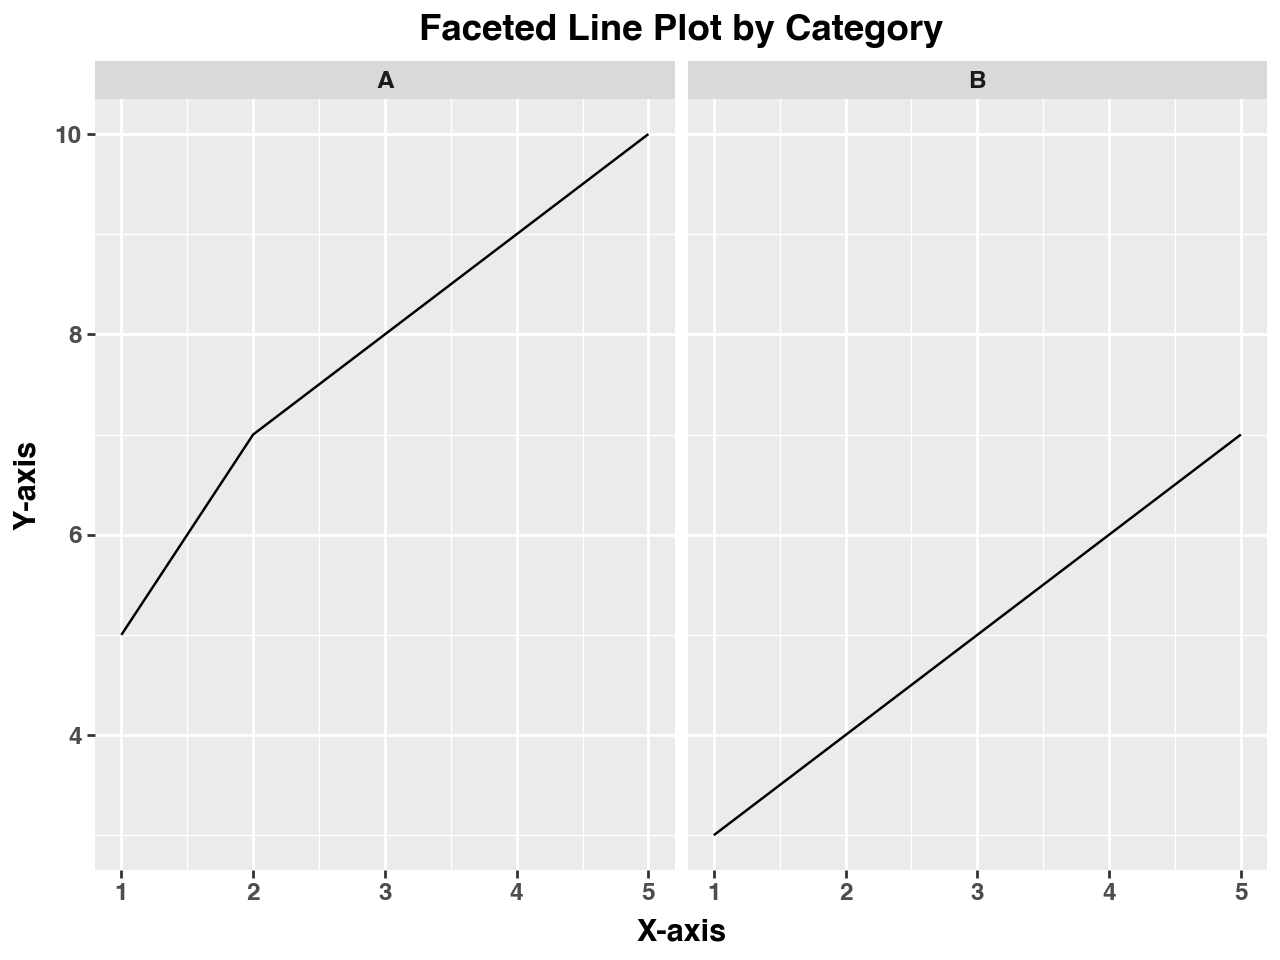
\includegraphics{15_Data_Vis_files/figure-pdf/cell-22-output-1.png}

}

\end{figure}

This example uses \texttt{facet\_wrap()} to create separate plots for
each category in the dataset, allowing for a clear visual comparison
between the groups.

\hypertarget{customizing-aesthetics-and-themes}{%
\subsection{Customizing Aesthetics and
Themes}\label{customizing-aesthetics-and-themes}}

Customization in \texttt{ggplot} extends beyond simple color and size
adjustments. The library allows for fine-tuning the plot's appearance
through themes, which can dramatically change the look and feel of your
visualizations.

\textbf{Example: Using a Different Theme}

\begin{Shaded}
\begin{Highlighting}[]
\ImportTok{from}\NormalTok{ plotnine }\ImportTok{import}\NormalTok{ theme\_minimal, theme\_bw}

\CommentTok{\# Applying a minimal theme to a scatter plot}
\NormalTok{(ggplot(scatter\_data, aes(x}\OperatorTok{=}\StringTok{\textquotesingle{}x\textquotesingle{}}\NormalTok{, y}\OperatorTok{=}\StringTok{\textquotesingle{}y\textquotesingle{}}\NormalTok{)) }\OperatorTok{+}
\NormalTok{ geom\_point(color}\OperatorTok{=}\StringTok{\textquotesingle{}blue\textquotesingle{}}\NormalTok{, size}\OperatorTok{=}\DecValTok{4}\NormalTok{) }\OperatorTok{+}
\NormalTok{ ggtitle(}\StringTok{\textquotesingle{}Scatter Plot with Minimal Theme\textquotesingle{}}\NormalTok{) }\OperatorTok{+}
\NormalTok{ xlab(}\StringTok{\textquotesingle{}X{-}axis Label\textquotesingle{}}\NormalTok{) }\OperatorTok{+}
\NormalTok{ ylab(}\StringTok{\textquotesingle{}Y{-}axis Label\textquotesingle{}}\NormalTok{) }\OperatorTok{+}
\NormalTok{ theme\_minimal())}
\end{Highlighting}
\end{Shaded}

\begin{figure}[H]

{\centering 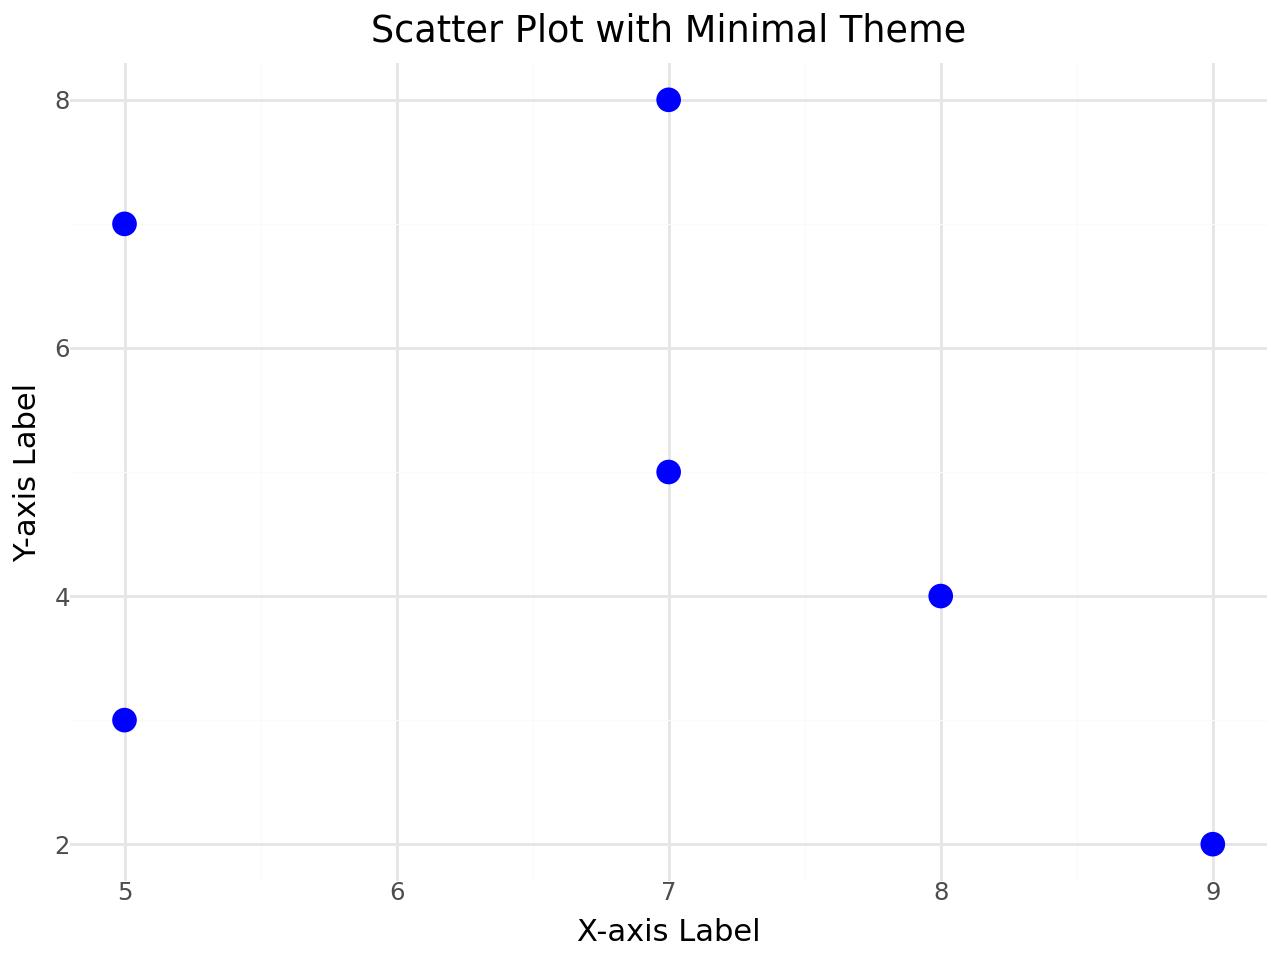
\includegraphics{15_Data_Vis_files/figure-pdf/cell-23-output-1.png}

}

\end{figure}

In this example, the \texttt{theme\_minimal()} function is applied to
give the plot a clean and modern look, with minimal grid lines and axis
labels.

\hypertarget{statistical-transformations}{%
\subsection{Statistical
Transformations}\label{statistical-transformations}}

\texttt{ggplot} in Python supports built-in statistical transformations
to highlight trends and patterns within the data. These transformations
can automatically compute summaries like smoothing lines or histograms.

\textbf{Example: Adding a Smoothing Line to a Scatter Plot}

\begin{Shaded}
\begin{Highlighting}[]
\ImportTok{from}\NormalTok{ plotnine }\ImportTok{import}\NormalTok{ geom\_smooth}

\CommentTok{\# Scatter plot with a smoothing line}
\NormalTok{(ggplot(scatter\_data, aes(x}\OperatorTok{=}\StringTok{\textquotesingle{}x\textquotesingle{}}\NormalTok{, y}\OperatorTok{=}\StringTok{\textquotesingle{}y\textquotesingle{}}\NormalTok{)) }\OperatorTok{+}
\NormalTok{ geom\_point(color}\OperatorTok{=}\StringTok{\textquotesingle{}red\textquotesingle{}}\NormalTok{, size}\OperatorTok{=}\DecValTok{3}\NormalTok{) }\OperatorTok{+}
\NormalTok{ geom\_smooth(method}\OperatorTok{=}\StringTok{\textquotesingle{}lm\textquotesingle{}}\NormalTok{, color}\OperatorTok{=}\StringTok{\textquotesingle{}blue\textquotesingle{}}\NormalTok{) }\OperatorTok{+}
\NormalTok{ ggtitle(}\StringTok{\textquotesingle{}Scatter Plot with Smoothing Line\textquotesingle{}}\NormalTok{) }\OperatorTok{+}
\NormalTok{ xlab(}\StringTok{\textquotesingle{}X{-}axis Label\textquotesingle{}}\NormalTok{) }\OperatorTok{+}
\NormalTok{ ylab(}\StringTok{\textquotesingle{}Y{-}axis Label\textquotesingle{}}\NormalTok{))}
\end{Highlighting}
\end{Shaded}

\begin{figure}[H]

{\centering 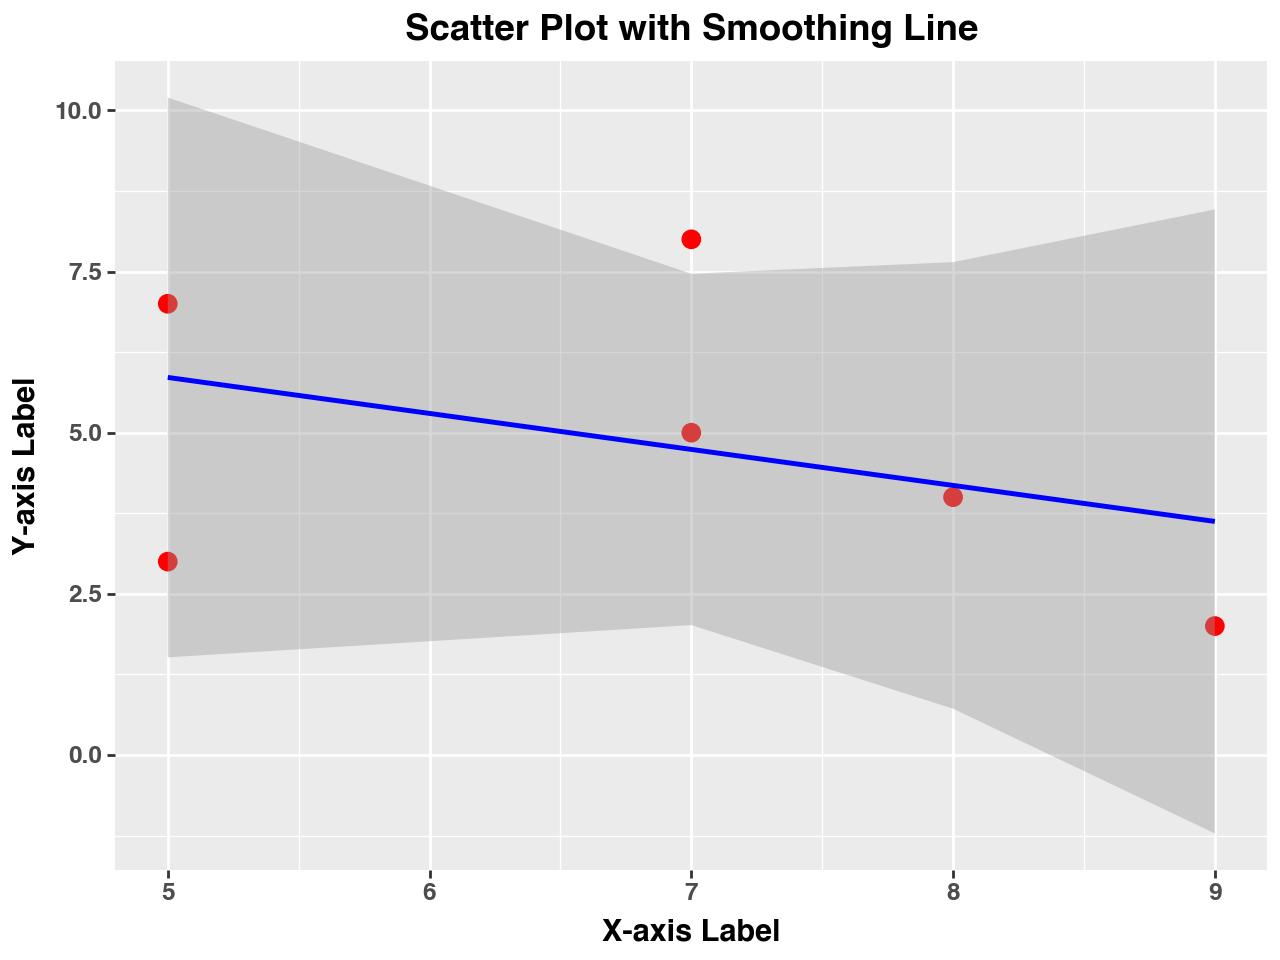
\includegraphics{15_Data_Vis_files/figure-pdf/cell-24-output-1.png}

}

\end{figure}

Here, \texttt{geom\_smooth()} adds a linear regression line to the
scatter plot, showing the trend in the data points.

\hypertarget{advantages-of-using-ggplot}{%
\subsection{Advantages of Using
ggplot}\label{advantages-of-using-ggplot}}

\begin{itemize}
\tightlist
\item
  \textbf{Consistency}: The grammar of graphics approach ensures that
  the process of building plots is systematic and repeatable.
\item
  \textbf{Customization}: Every aspect of the plot can be adjusted to
  suit specific needs or aesthetic preferences.
\item
  \textbf{Layered Design}: Allows for easy addition and modification of
  plot components without altering the underlying structure.
\item
  \textbf{Built-In Statistical Tools}: Supports automatic statistical
  transformations to help identify patterns in the data.
\end{itemize}

\hypertarget{limitations-and-considerations-1}{%
\subsection{Limitations and
Considerations}\label{limitations-and-considerations-1}}

While \texttt{ggplot} offers great flexibility and aesthetic appeal,
there are some considerations to keep in mind:

\begin{itemize}
\tightlist
\item
  \textbf{Performance}: Rendering complex visualizations with large
  datasets can be slower compared to other libraries.
\item
  \textbf{Learning Curve}: Requires a solid understanding of the grammar
  of graphics concepts, which might be challenging for beginners.
\item
  \textbf{Dependencies}: As a port of ggplot2 from R, some features
  might differ or be less developed than in the R version.
\end{itemize}

\hypertarget{exercises-11}{%
\section{Exercises}\label{exercises-11}}

\hypertarget{exercise-1-working-with-matplotlib---creating-basic-line-plots}{%
\subsubsection{Exercise 1: Working with Matplotlib - Creating Basic Line
Plots}\label{exercise-1-working-with-matplotlib---creating-basic-line-plots}}

\begin{itemize}
\item
  Using Matplotlib, create a line plot of the function \(f(x) = x^2\)
  for \(x\) values ranging from -10 to 10. Customize the plot by adding
  labels to the axes, a title, and a grid.
\item
  Modify your plot to change the line color to red and use a dashed line
  style. Add circular markers to each data point.
\end{itemize}

\hypertarget{exercise-2-working-with-matplotlib---scatter-plot-customization}{%
\subsubsection{Exercise 2: Working with Matplotlib - Scatter Plot
Customization}\label{exercise-2-working-with-matplotlib---scatter-plot-customization}}

\begin{itemize}
\item
  Generate a scatter plot using the following data:

  \begin{itemize}
  \tightlist
  \item
    \(x = [2, 4, 6, 8, 10]\)
  \item
    \(y = [1, 4, 9, 16, 25]\)
  \end{itemize}
\item
  Customize the scatter plot by using triangle markers, coloring the
  points green, and increasing the marker size. Label the axes and add a
  title to the plot.
\end{itemize}

\hypertarget{exercise-3-working-with-matplotlib---creating-subplots}{%
\subsubsection{Exercise 3: Working with Matplotlib - Creating
Subplots}\label{exercise-3-working-with-matplotlib---creating-subplots}}

\begin{itemize}
\item
  Create a figure with two subplots arranged vertically:

  \begin{itemize}
  \item
    The first subplot should be a line plot of \(f(x) = x^3\) for \(x\)
    values from -5 to 5.
  \item
    The second subplot should be a scatter plot of the points
    \((-3, -27)\), \((-2, -8)\), \((0, 0)\), \((2, 8)\), and
    \((3, 27)\).
  \end{itemize}
\item
  Ensure that each subplot has a title and labeled axes, and adjust the
  spacing between the plots for better readability.
\end{itemize}

\hypertarget{exercise-4-advanced-data-visualization-with-seaborn---analyzing-data-distributions}{%
\subsubsection{Exercise 4: Advanced Data Visualization with Seaborn -
Analyzing Data
Distributions}\label{exercise-4-advanced-data-visualization-with-seaborn---analyzing-data-distributions}}

\begin{itemize}
\item
  Load the built-in \texttt{tips} dataset from Seaborn. Create a
  histogram of the \texttt{total\_bill} variable with a KDE (Kernel
  Density Estimate) overlay. Customize the color of the histogram and
  KDE line.
\item
  Interpret the resulting plot, describing any noticeable patterns in
  the distribution of the \texttt{total\_bill} values.
\end{itemize}

\hypertarget{exercise-5-advanced-data-visualization-with-seaborn---comparing-categorical-data}{%
\subsubsection{Exercise 5: Advanced Data Visualization with Seaborn -
Comparing Categorical
Data}\label{exercise-5-advanced-data-visualization-with-seaborn---comparing-categorical-data}}

\begin{itemize}
\item
  Using the \texttt{tips} dataset, create a box plot to visualize the
  distribution of tips received by day of the week. Differentiate
  between smokers and non-smokers using the \texttt{hue} parameter.
\item
  Analyze the box plot to determine on which day the highest median tip
  amount is given and whether smokers tend to tip more than non-smokers.
\end{itemize}

\hypertarget{exercise-6-advanced-data-visualization-with-seaborn---correlation-analysis-with-heatmaps}{%
\subsubsection{Exercise 6: Advanced Data Visualization with Seaborn -
Correlation Analysis with
Heatmaps}\label{exercise-6-advanced-data-visualization-with-seaborn---correlation-analysis-with-heatmaps}}

\begin{itemize}
\item
  Generate a heatmap showing the correlation matrix of the numerical
  variables in the \texttt{tips} dataset. Use the \texttt{coolwarm}
  color palette and display the correlation values on the heatmap.
\item
  Based on the heatmap, identify which two variables have the strongest
  correlation and describe their relationship.
\end{itemize}

\hypertarget{exercise-7-exploring-ggplot-with-plotnine---basic-line-plot-with-ggplot}{%
\subsubsection{Exercise 7: Exploring ggplot with plotnine - Basic Line
Plot with
ggplot}\label{exercise-7-exploring-ggplot-with-plotnine---basic-line-plot-with-ggplot}}

\begin{itemize}
\item
  Using the \texttt{plotnine} package, create a basic line plot of the
  function \(g(x) = \sin(x)\) for \(x\) values ranging from 0 to
  \(2\pi\). Add appropriate labels to the axes and a title to the plot.
\item
  Enhance the plot by adding points at each integer value of \(x\) with
  different color markers.
\end{itemize}

\hypertarget{exercise-8-exploring-ggplot-with-plotnine---creating-faceted-plots}{%
\subsubsection{Exercise 8: Exploring ggplot with plotnine - Creating
Faceted
Plots}\label{exercise-8-exploring-ggplot-with-plotnine---creating-faceted-plots}}

\begin{itemize}
\item
  Create a dataset with two groups, ``A'' and ``B'', and plot a faceted
  line plot using \texttt{ggplot}. Plot the following data points:

  \begin{itemize}
  \tightlist
  \item
    Group A: \((1, 2)\), \((2, 4)\), \((3, 8)\), \((4, 16)\)
  \item
    Group B: \((1, 1)\), \((2, 2)\), \((3, 3)\), \((4, 4)\)
  \end{itemize}
\item
  Use facetting to display each group's plot in a separate subplot and
  ensure that both plots share the same x-axis and y-axis labels.
\end{itemize}

\hypertarget{exercise-9-exploring-ggplot-with-plotnine---applying-themes-and-aesthetic-modifications}{%
\subsubsection{Exercise 9: Exploring ggplot with plotnine - Applying
Themes and Aesthetic
Modifications}\label{exercise-9-exploring-ggplot-with-plotnine---applying-themes-and-aesthetic-modifications}}

\begin{itemize}
\item
  Create a scatter plot using \texttt{ggplot} with a dataset of your
  choice. Apply the \texttt{theme\_minimal} style and modify the
  aesthetics by changing the point color, size, and adding a smooth line
  to represent the trend in the data.
\item
  Save your plot as a PNG file with a resolution of 300 dpi.
\end{itemize}

\bookmarksetup{startatroot}

\hypertarget{sec-oop}{%
\chapter{Object-Oriented Programming in Python}\label{sec-oop}}

\hypertarget{introduction-to-object-oriented-programming}{%
\section{Introduction to Object-Oriented
Programming}\label{introduction-to-object-oriented-programming}}

Object-Oriented Programming (OOP) is a programming paradigm that models
real-world entities using objects and classes. While procedural
programming focuses on functions and the sequence of operations, OOP
centers around organizing code into objects, which encapsulate both data
and behavior. This approach makes it easier to manage, extend, and
modify large and complex programs, while also allowing for better reuse
of code.

To understand OOP at a conceptual level, it can be helpful to look at
examples from everyday life. These examples will illustrate the key
concepts of OOP: \textbf{classes}, \textbf{objects},
\textbf{attributes}, and \textbf{methods}. Later in this chapter, we
will see how these ideas map onto programming.

\hypertarget{objects-and-classes-in-everyday-life}{%
\subsection{Objects and Classes in Everyday
Life}\label{objects-and-classes-in-everyday-life}}

Imagine you're organizing a car dealership. Every car on the lot can be
seen as an \textbf{object}---a specific instance of a general concept,
such as a car. The general concept is what we refer to as a
\textbf{class} in OOP. A class acts like a blueprint or template for
creating objects. Each car on the lot is unique in some way, but they
all share certain common traits and behaviors, just like objects created
from a class.

Let's break this down:

\begin{itemize}
\tightlist
\item
  \textbf{Class}: A car can be described by a blueprint, which details
  its general characteristics (such as make, model, engine type, etc.)
  and behaviors (like starting the engine, honking the horn). In OOP,
  this blueprint is the \textbf{class}.
\item
  \textbf{Object}: Each specific car you have on the lot---a 2021 Toyota
  Camry, a 2020 Honda Civic, etc.---is an \textbf{object} created from
  the class blueprint. These cars have specific values for their
  characteristics (for example, one car is blue, another has a sunroof).
\end{itemize}

This distinction between class and object is fundamental to OOP. A
\textbf{class} provides the general description, while an
\textbf{object} is a specific instance created from that description.

\hypertarget{attributes-and-methods}{%
\subsection{Attributes and Methods}\label{attributes-and-methods}}

Objects have \textbf{attributes} and \textbf{methods}. Attributes are
the data that describe the state of an object, while methods are the
actions or behaviors an object can perform.

Continuing with our car dealership analogy:

\begin{itemize}
\tightlist
\item
  \textbf{Attributes}: Each car has specific properties like color,
  make, model, year, and mileage. These properties are the
  \textbf{attributes} of the car object.
\item
  \textbf{Methods}: The behaviors of a car, such as starting the engine,
  honking the horn, or accelerating, are the \textbf{methods}. In the
  class blueprint, methods describe what a car can do, and in OOP terms,
  they are the actions or functions that can be performed on or by an
  object.
\end{itemize}

Just as a car's attributes are set when the car is manufactured, an
object's attributes are defined when the object is created from the
class.

\hypertarget{example-oop-in-a-library-system}{%
\subsubsection{Example: OOP in a Library
System}\label{example-oop-in-a-library-system}}

Consider a library system, which can also be modeled using OOP
principles. In this case, \textbf{books} are objects, and
\textbf{LibraryBook} might be the class that defines their shared
characteristics and behaviors.

\begin{itemize}
\tightlist
\item
  \textbf{Class (LibraryBook)}: The class defines the general properties
  of a book, such as its title, author, publication date, and ISBN. It
  also defines behaviors, such as checking the book out or returning it.
\item
  \textbf{Objects}: Each specific book in the library---like ``To Kill a
  Mockingbird'' or ``Pride and Prejudice''---is an object created from
  the \textbf{LibraryBook} class. Each object has specific values for
  its attributes (e.g., title, author) but shares the same behaviors
  (e.g., can be checked out or returned).
\end{itemize}

When you borrow a book from the library, the system doesn't just perform
random tasks; it interacts with the specific book object, checking if it
is available or already checked out. This interaction between the object
and its methods is one of the strengths of OOP---it provides a
structured and organized way to manage complex systems.

\hypertarget{encapsulation-keeping-attributes-and-methods-together}{%
\subsection{Encapsulation: Keeping Attributes and Methods
Together}\label{encapsulation-keeping-attributes-and-methods-together}}

One of the key advantages of OOP is \textbf{encapsulation}---the concept
of bundling data (attributes) and behaviors (methods) together in one
entity, the object. This allows for better organization and modularity.

Let's return to our car example: You can think of each car as a
self-contained object. If you want to interact with the car, you don't
need to know every intricate detail about its inner workings; you just
need to use the car's methods. For instance, to start the car, you don't
have to understand how the engine works---you just turn the key or press
a button, and the car performs the appropriate behavior.

In programming, encapsulation works in a similar way. When a class is
designed, its internal workings (the code and data) are hidden from
other parts of the program. Instead, the class provides a clear
interface (methods) that can be used to interact with its objects. This
hiding of internal details makes the system easier to maintain and
modify, because changes to the internal structure of a class won't
affect the rest of the program as long as the interface remains the
same.

\hypertarget{real-world-example-a-bank-account-system}{%
\subsubsection{Real-World Example: A Bank Account
System}\label{real-world-example-a-bank-account-system}}

Consider a \textbf{BankAccount} class in an online banking system. This
class defines the shared characteristics of all bank accounts (e.g.,
account number, balance) and the behaviors that all accounts can perform
(e.g., deposit money, withdraw money, check balance).

\begin{itemize}
\tightlist
\item
  \textbf{Class (BankAccount)}: This acts as the blueprint for creating
  specific bank accounts. It defines that each account will have an
  account number, a balance, and methods to deposit or withdraw funds.
\item
  \textbf{Objects}: Each customer's bank account is an object created
  from the BankAccount class. For example, one object might represent
  Alice's bank account, while another represents Bob's bank account.
\end{itemize}

The concept of encapsulation is crucial here. You, as the user of the
bank account, don't need to know how the bank stores your balance or how
it processes withdrawals internally. All you need to know is that when
you call the \texttt{deposit()} method, money is added to your account,
and when you call the \texttt{withdraw()} method, money is subtracted.
The internal details (data storage, security checks) are hidden from
you.

This separation of concerns allows bank developers to modify the
internal workings of the bank system without affecting the customers'
interactions. For example, the bank might switch to a more efficient
algorithm for handling transactions, but as long as the deposit and
withdraw methods work the same way, the change is invisible to the user.

\hypertarget{why-use-oop}{%
\subsection{Why Use OOP?}\label{why-use-oop}}

Now that we've seen how OOP relates to real-world examples, let's
summarize why this approach is so beneficial in programming:

\begin{enumerate}
\def\labelenumi{\arabic{enumi}.}
\item
  \textbf{Modularity and Reusability}: By encapsulating data and
  behavior within classes, OOP promotes modular code that can be reused
  across different programs. For instance, a class written to represent
  a ``student'' in a school system can be reused in other systems (e.g.,
  a library system).
\item
  \textbf{Ease of Maintenance}: Because objects are self-contained and
  interact with the rest of the system through defined methods, changes
  to one part of the system are less likely to break the entire program.
  This makes OOP programs easier to maintain and scale.
\item
  \textbf{Flexibility Through Inheritance}: OOP allows classes to be
  extended and specialized through inheritance, a powerful feature that
  we will discuss in detail later. This allows for the creation of
  complex systems that can be easily modified and extended.
\item
  \textbf{Real-World Modeling}: OOP allows programmers to model
  real-world systems in a way that's intuitive and easy to understand.
  Objects in OOP can directly correspond to real-world entities, making
  the design and development process more natural.
\end{enumerate}

In the next section, we will explore how to define a class in Python,
bringing these concepts into the programming world and showing how to
create and work with objects.

\hypertarget{defining-a-class}{%
\section{Defining a Class}\label{defining-a-class}}

Now that we've explored the key concepts behind Object-Oriented
Programming (OOP) and how they relate to everyday examples, it's time to
move into the practical side: defining a class in Python. A class is the
fundamental building block of OOP, serving as the blueprint for creating
objects. Each object created from a class shares the structure and
behavior defined by that class, but with unique values for its
attributes.

In this section, we will dive into the syntax of class definition in
Python, demonstrate how to create classes, and explain how attributes
and methods are defined within a class. As you go through this section,
keep in mind the real-world analogies from the previous section to
understand how Python classes mimic real-world entities.

\hypertarget{basic-class-syntax}{%
\subsection{Basic Class Syntax}\label{basic-class-syntax}}

In Python, defining a class is straightforward. The keyword
\texttt{class} is used, followed by the class name and a colon. The body
of the class contains the attributes (data) and methods (functions) that
define the behavior of objects created from the class.

Here's a simple example:

\begin{Shaded}
\begin{Highlighting}[]
\KeywordTok{class}\NormalTok{ Car:}
    \ControlFlowTok{pass}
\end{Highlighting}
\end{Shaded}

This is the simplest possible class definition: a class named
\texttt{Car} with no attributes or methods. The keyword \texttt{pass} is
used as a placeholder, indicating that there is no functionality yet. We
will build on this example to make it more meaningful.

\hypertarget{the-__init__-method-class-constructor}{%
\subsection{\texorpdfstring{The \texttt{\_\_init\_\_} Method: Class
Constructor}{The \_\_init\_\_ Method: Class Constructor}}\label{the-__init__-method-class-constructor}}

In most cases, you'll want your class to initialize some values when an
object is created. This is where the \texttt{\_\_init\_\_} method comes
into play. The \texttt{\_\_init\_\_} method is known as the
\textbf{constructor}, and it is automatically called when an object is
instantiated from the class. It is used to set up initial values for the
object's attributes.

Let's expand on our \texttt{Car} class:

\begin{Shaded}
\begin{Highlighting}[]
\KeywordTok{class}\NormalTok{ Car:}
    \KeywordTok{def} \FunctionTok{\_\_init\_\_}\NormalTok{(}\VariableTok{self}\NormalTok{, make, model, year):}
        \VariableTok{self}\NormalTok{.make }\OperatorTok{=}\NormalTok{ make}
        \VariableTok{self}\NormalTok{.model }\OperatorTok{=}\NormalTok{ model}
        \VariableTok{self}\NormalTok{.year }\OperatorTok{=}\NormalTok{ year}
\end{Highlighting}
\end{Shaded}

Here's what's happening:

\begin{itemize}
\tightlist
\item
  The \texttt{\_\_init\_\_} method takes several arguments:
  \texttt{self}, \texttt{make}, \texttt{model}, and \texttt{year}.
\item
  \texttt{self} refers to the specific object being created. It allows
  you to assign the values to the object's attributes.
\item
  Inside the method, \texttt{self.make}, \texttt{self.model}, and
  \texttt{self.year} refer to the attributes of the object. We assign
  the values passed in (\texttt{make}, \texttt{model}, and
  \texttt{year}) to those attributes.
\end{itemize}

This way, each object (or instance) of the \texttt{Car} class will have
its own \texttt{make}, \texttt{model}, and \texttt{year} attributes,
which are set when the object is created.

\hypertarget{example-creating-objects-from-a-class}{%
\subsubsection{Example: Creating Objects from a
Class}\label{example-creating-objects-from-a-class}}

Let's create some \texttt{Car} objects using this class:

\begin{Shaded}
\begin{Highlighting}[]
\NormalTok{car1 }\OperatorTok{=}\NormalTok{ Car(}\StringTok{"Toyota"}\NormalTok{, }\StringTok{"Camry"}\NormalTok{, }\DecValTok{2021}\NormalTok{)}
\NormalTok{car2 }\OperatorTok{=}\NormalTok{ Car(}\StringTok{"Honda"}\NormalTok{, }\StringTok{"Civic"}\NormalTok{, }\DecValTok{2020}\NormalTok{)}

\BuiltInTok{print}\NormalTok{(car1.make)  }
\BuiltInTok{print}\NormalTok{(car2.year)  }
\end{Highlighting}
\end{Shaded}

\begin{verbatim}
Toyota
2020
\end{verbatim}

Here, \texttt{car1} and \texttt{car2} are objects created from the
\texttt{Car} class. Each object has its own set of attributes:
\texttt{car1} is a Toyota Camry from 2021, and \texttt{car2} is a Honda
Civic from 2020. We can access these attributes using dot notation
(\texttt{car1.make}, \texttt{car2.year}).

This structure mirrors real-world examples: just as each car in a
dealership has specific properties, each object in OOP has specific
values for its attributes, even though they are all created from the
same class blueprint.

\hypertarget{methods-and-attributes-in-a-class}{%
\section{Methods and Attributes in a
Class}\label{methods-and-attributes-in-a-class}}

In addition to attributes, a class can define
\textbf{methods}---functions that describe the behaviors or actions the
objects can perform. Methods in a class always take \texttt{self} as the
first argument, which refers to the instance on which the method is
being called.

Let's add a method to the \texttt{Car} class that allows the car to
display its full description:

\begin{Shaded}
\begin{Highlighting}[]
\KeywordTok{class}\NormalTok{ Car:}
    \KeywordTok{def} \FunctionTok{\_\_init\_\_}\NormalTok{(}\VariableTok{self}\NormalTok{, make, model, year):}
        \VariableTok{self}\NormalTok{.make }\OperatorTok{=}\NormalTok{ make}
        \VariableTok{self}\NormalTok{.model }\OperatorTok{=}\NormalTok{ model}
        \VariableTok{self}\NormalTok{.year }\OperatorTok{=}\NormalTok{ year}

    \KeywordTok{def}\NormalTok{ description(}\VariableTok{self}\NormalTok{):}
        \ControlFlowTok{return} \SpecialStringTok{f"}\SpecialCharTok{\{}\VariableTok{self}\SpecialCharTok{.}\NormalTok{year}\SpecialCharTok{\}}\SpecialStringTok{ }\SpecialCharTok{\{}\VariableTok{self}\SpecialCharTok{.}\NormalTok{make}\SpecialCharTok{\}}\SpecialStringTok{ }\SpecialCharTok{\{}\VariableTok{self}\SpecialCharTok{.}\NormalTok{model}\SpecialCharTok{\}}\SpecialStringTok{"}
\end{Highlighting}
\end{Shaded}

In this example, the method \texttt{description} returns a formatted
string with the car's year, make, and model.

\begin{Shaded}
\begin{Highlighting}[]
\NormalTok{car1 }\OperatorTok{=}\NormalTok{ Car(}\StringTok{"Toyota"}\NormalTok{, }\StringTok{"Camry"}\NormalTok{, }\DecValTok{2021}\NormalTok{)}
\BuiltInTok{print}\NormalTok{(car1.description())  }
\end{Highlighting}
\end{Shaded}

\begin{verbatim}
2021 Toyota Camry
\end{verbatim}

Here, we define the method \texttt{description} inside the class. When
we call \texttt{car1.description()}, the car provides its full
description. This method operates on the instance of the class (e.g.,
\texttt{car1}), and it has access to the attributes via \texttt{self}.

\hypertarget{instance-attributes-vs.-class-attributes}{%
\subsection{Instance Attributes vs.~Class
Attributes}\label{instance-attributes-vs.-class-attributes}}

In Python, attributes can be classified into two types: \textbf{instance
attributes} and \textbf{class attributes}.

\begin{itemize}
\item
  \textbf{Instance Attributes}: These are specific to each object and
  are defined inside the \texttt{\_\_init\_\_} method. For example, in
  the \texttt{Car} class, \texttt{make}, \texttt{model}, and
  \texttt{year} are instance attributes. Each car object has its own
  unique values for these attributes.
\item
  \textbf{Class Attributes}: These are shared across all instances of a
  class. They are defined directly within the class but outside of any
  method. All objects of the class will share the same value for a class
  attribute, unless it is explicitly overridden in an instance.
\end{itemize}

Let's modify the \texttt{Car} class to include a class attribute:

\begin{Shaded}
\begin{Highlighting}[]
\KeywordTok{class}\NormalTok{ Car:}
\NormalTok{    wheels }\OperatorTok{=} \DecValTok{4}  \CommentTok{\# Class attribute}

    \KeywordTok{def} \FunctionTok{\_\_init\_\_}\NormalTok{(}\VariableTok{self}\NormalTok{, make, model, year):}
        \VariableTok{self}\NormalTok{.make }\OperatorTok{=}\NormalTok{ make}
        \VariableTok{self}\NormalTok{.model }\OperatorTok{=}\NormalTok{ model}
        \VariableTok{self}\NormalTok{.year }\OperatorTok{=}\NormalTok{ year}

    \KeywordTok{def}\NormalTok{ description(}\VariableTok{self}\NormalTok{):}
        \ControlFlowTok{return} \SpecialStringTok{f"}\SpecialCharTok{\{}\VariableTok{self}\SpecialCharTok{.}\NormalTok{year}\SpecialCharTok{\}}\SpecialStringTok{ }\SpecialCharTok{\{}\VariableTok{self}\SpecialCharTok{.}\NormalTok{make}\SpecialCharTok{\}}\SpecialStringTok{ }\SpecialCharTok{\{}\VariableTok{self}\SpecialCharTok{.}\NormalTok{model}\SpecialCharTok{\}}\SpecialStringTok{"}
\end{Highlighting}
\end{Shaded}

In this case, \texttt{wheels} is a class attribute, meaning that all
cars created from the \texttt{Car} class will have 4 wheels. This
attribute is shared among all instances of the class:

\begin{Shaded}
\begin{Highlighting}[]
\NormalTok{car1 }\OperatorTok{=}\NormalTok{ Car(}\StringTok{"Toyota"}\NormalTok{, }\StringTok{"Camry"}\NormalTok{, }\DecValTok{2021}\NormalTok{)}
\NormalTok{car2 }\OperatorTok{=}\NormalTok{ Car(}\StringTok{"Honda"}\NormalTok{, }\StringTok{"Civic"}\NormalTok{, }\DecValTok{2020}\NormalTok{)}

\BuiltInTok{print}\NormalTok{(car1.wheels)  }
\BuiltInTok{print}\NormalTok{(car2.wheels)  }
\end{Highlighting}
\end{Shaded}

\begin{verbatim}
4
4
\end{verbatim}

Class attributes can be useful for defining properties that are the same
across all instances, such as the number of wheels for cars.

\hypertarget{modifying-attributes}{%
\subsection{Modifying Attributes}\label{modifying-attributes}}

It is possible to modify both instance and class attributes after an
object has been created. Let's see how this works.

\hypertarget{modifying-instance-attributes}{%
\subsubsection{Modifying Instance
Attributes}\label{modifying-instance-attributes}}

\begin{Shaded}
\begin{Highlighting}[]
\NormalTok{car1 }\OperatorTok{=}\NormalTok{ Car(}\StringTok{"Toyota"}\NormalTok{, }\StringTok{"Camry"}\NormalTok{, }\DecValTok{2021}\NormalTok{)}
\BuiltInTok{print}\NormalTok{(car1.description())  }

\CommentTok{\# Modifying the year}
\NormalTok{car1.year }\OperatorTok{=} \DecValTok{2022}
\BuiltInTok{print}\NormalTok{(car1.description())  }
\end{Highlighting}
\end{Shaded}

\begin{verbatim}
2021 Toyota Camry
2022 Toyota Camry
\end{verbatim}

Here, we update the \texttt{year} attribute for \texttt{car1}, and the
object reflects the new value when we call the \texttt{description}
method again.

\hypertarget{modifying-class-attributes}{%
\subsubsection{Modifying Class
Attributes}\label{modifying-class-attributes}}

Class attributes can be modified directly using the class name. Any
change to a class attribute will be reflected across all instances of
the class:

\begin{Shaded}
\begin{Highlighting}[]
\NormalTok{Car.wheels }\OperatorTok{=} \DecValTok{3}
\BuiltInTok{print}\NormalTok{(car1.wheels)}
\end{Highlighting}
\end{Shaded}

\begin{verbatim}
3
\end{verbatim}

By modifying the \texttt{wheels} class attribute, we've updated the
number of wheels for all \texttt{Car} objects.

\hypertarget{inheritance}{%
\section{Inheritance}\label{inheritance}}

Inheritance is one of the most powerful features of Object-Oriented
Programming (OOP). It allows a new class to inherit the properties and
behaviors (attributes and methods) of an existing class. The new class,
known as the \textbf{subclass} or \textbf{child class}, can also have
additional attributes and methods or override existing ones from the
parent class. This promotes code reuse and makes it easier to build
complex systems by extending functionality rather than starting from
scratch.

To understand inheritance conceptually, let's once again consider some
real-world examples.

\hypertarget{inheritance-in-everyday-life}{%
\subsection{Inheritance in Everyday
Life}\label{inheritance-in-everyday-life}}

Imagine a university system where you have \textbf{students} and
\textbf{graduate students}. Both graduate and undergraduate students
share many characteristics: they have a name, student ID, and GPA.
However, graduate students also have some unique attributes, such as a
thesis title and an advisor. It would be redundant to create separate
classes for students and graduate students from scratch because many of
their attributes overlap.

Instead, we can create a general \textbf{Student} class and a more
specialized \textbf{GraduateStudent} class. The GraduateStudent class
can inherit the common attributes and behaviors from the Student class,
while adding its own unique features. This hierarchical structure is a
natural fit for OOP and is made possible through inheritance.

\hypertarget{defining-inheritance-in-python}{%
\subsection{Defining Inheritance in
Python}\label{defining-inheritance-in-python}}

In Python, inheritance is defined by specifying the parent class in
parentheses when defining the child class. The child class inherits all
the attributes and methods from the parent class.

Let's define a basic example:

\begin{Shaded}
\begin{Highlighting}[]
\KeywordTok{class}\NormalTok{ Student:}
    \KeywordTok{def} \FunctionTok{\_\_init\_\_}\NormalTok{(}\VariableTok{self}\NormalTok{, name, student\_id, gpa):}
        \VariableTok{self}\NormalTok{.name }\OperatorTok{=}\NormalTok{ name}
        \VariableTok{self}\NormalTok{.student\_id }\OperatorTok{=}\NormalTok{ student\_id}
        \VariableTok{self}\NormalTok{.gpa }\OperatorTok{=}\NormalTok{ gpa}

    \KeywordTok{def}\NormalTok{ display\_info(}\VariableTok{self}\NormalTok{):}
        \ControlFlowTok{return} \SpecialStringTok{f"Student: }\SpecialCharTok{\{}\VariableTok{self}\SpecialCharTok{.}\NormalTok{name}\SpecialCharTok{\}}\SpecialStringTok{, ID: }\SpecialCharTok{\{}\VariableTok{self}\SpecialCharTok{.}\NormalTok{student\_id}\SpecialCharTok{\}}\SpecialStringTok{, GPA: }\SpecialCharTok{\{}\VariableTok{self}\SpecialCharTok{.}\NormalTok{gpa}\SpecialCharTok{\}}\SpecialStringTok{"}
\end{Highlighting}
\end{Shaded}

Here, the \texttt{Student} class defines three attributes
(\texttt{name}, \texttt{student\_id}, and \texttt{gpa}) and one method
(\texttt{display\_info}). Now, we will define a subclass,
\texttt{GraduateStudent}, which will inherit from \texttt{Student}.

\begin{Shaded}
\begin{Highlighting}[]
\KeywordTok{class}\NormalTok{ GraduateStudent(Student):}
    \KeywordTok{def} \FunctionTok{\_\_init\_\_}\NormalTok{(}\VariableTok{self}\NormalTok{, name, student\_id, gpa, thesis\_title):}
        \BuiltInTok{super}\NormalTok{().}\FunctionTok{\_\_init\_\_}\NormalTok{(name, student\_id, gpa)}
        \VariableTok{self}\NormalTok{.thesis\_title }\OperatorTok{=}\NormalTok{ thesis\_title}

    \KeywordTok{def}\NormalTok{ display\_thesis(}\VariableTok{self}\NormalTok{):}
        \ControlFlowTok{return} \SpecialStringTok{f"Thesis: }\SpecialCharTok{\{}\VariableTok{self}\SpecialCharTok{.}\NormalTok{thesis\_title}\SpecialCharTok{\}}\SpecialStringTok{"}
\end{Highlighting}
\end{Shaded}

In this example:

\begin{itemize}
\tightlist
\item
  The \texttt{GraduateStudent} class inherits from \texttt{Student}. We
  can see this by the syntax \texttt{class\ GraduateStudent(Student)}.
\item
  The \texttt{\_\_init\_\_} method of the \texttt{GraduateStudent} class
  uses \texttt{super().\_\_init\_\_()} to call the parent class's
  constructor, inheriting the initialization of \texttt{name},
  \texttt{student\_id}, and \texttt{gpa}.
\item
  A new attribute, \texttt{thesis\_title}, is added, along with a method
  \texttt{display\_thesis()} to show the thesis title.
\end{itemize}

\hypertarget{example-creating-instances-of-subclasses}{%
\subsubsection{Example: Creating Instances of
Subclasses}\label{example-creating-instances-of-subclasses}}

Now let's create instances of the \texttt{Student} and
\texttt{GraduateStudent} classes to see how inheritance works in
practice:

\begin{Shaded}
\begin{Highlighting}[]
\CommentTok{\# Creating a Student object}
\NormalTok{student1 }\OperatorTok{=}\NormalTok{ Student(}\StringTok{"Alice"}\NormalTok{, }\StringTok{"S12345"}\NormalTok{, }\FloatTok{3.9}\NormalTok{)}
\BuiltInTok{print}\NormalTok{(student1.display\_info())  }

\CommentTok{\# Creating a GraduateStudent object}
\NormalTok{grad\_student1 }\OperatorTok{=}\NormalTok{ GraduateStudent(}\StringTok{"Bob"}\NormalTok{, }\StringTok{"G54321"}\NormalTok{, }\FloatTok{4.0}\NormalTok{, }\StringTok{"Quantum Computing"}\NormalTok{)}
\BuiltInTok{print}\NormalTok{(grad\_student1.display\_info())  }

\BuiltInTok{print}\NormalTok{(grad\_student1.display\_thesis())  }
\end{Highlighting}
\end{Shaded}

\begin{verbatim}
Student: Alice, ID: S12345, GPA: 3.9
Student: Bob, ID: G54321, GPA: 4.0
Thesis: Quantum Computing
\end{verbatim}

As shown, \texttt{GraduateStudent} inherits the \texttt{display\_info()}
method from the \texttt{Student} class, and we can also use the
\texttt{display\_thesis()} method that is specific to
\texttt{GraduateStudent}.

\hypertarget{overriding-methods}{%
\subsection{Overriding Methods}\label{overriding-methods}}

One of the most useful aspects of inheritance is the ability to override
methods from the parent class in the child class. This allows the child
class to modify or extend the behavior of a method without affecting the
parent class.

Let's say we want the \texttt{GraduateStudent} class to display more
detailed information about the student, including the thesis title, when
calling the \texttt{display\_info()} method. We can override this method
in the \texttt{GraduateStudent} class:

\begin{Shaded}
\begin{Highlighting}[]
\KeywordTok{class}\NormalTok{ GraduateStudent(Student):}
    \KeywordTok{def} \FunctionTok{\_\_init\_\_}\NormalTok{(}\VariableTok{self}\NormalTok{, name, student\_id, gpa, thesis\_title):}
        \BuiltInTok{super}\NormalTok{().}\FunctionTok{\_\_init\_\_}\NormalTok{(name, student\_id, gpa)}
        \VariableTok{self}\NormalTok{.thesis\_title }\OperatorTok{=}\NormalTok{ thesis\_title}

    \CommentTok{\# Overriding the display\_info method}
    \KeywordTok{def}\NormalTok{ display\_info(}\VariableTok{self}\NormalTok{):}
        \ControlFlowTok{return} \SpecialStringTok{f"Graduate Student: }\SpecialCharTok{\{}\VariableTok{self}\SpecialCharTok{.}\NormalTok{name}\SpecialCharTok{\}}\SpecialStringTok{, ID: }\SpecialCharTok{\{}\VariableTok{self}\SpecialCharTok{.}\NormalTok{student\_id}\SpecialCharTok{\}}\SpecialStringTok{, GPA: }\SpecialCharTok{\{}\VariableTok{self}\SpecialCharTok{.}\NormalTok{gpa}\SpecialCharTok{\}}\SpecialStringTok{, Thesis: }\SpecialCharTok{\{}\VariableTok{self}\SpecialCharTok{.}\NormalTok{thesis\_title}\SpecialCharTok{\}}\SpecialStringTok{"}
\end{Highlighting}
\end{Shaded}

Now, when \texttt{display\_info()} is called on a
\texttt{GraduateStudent} object, it uses the overridden version of the
method instead of the parent class's version:

\begin{Shaded}
\begin{Highlighting}[]
\NormalTok{grad\_student1 }\OperatorTok{=}\NormalTok{ GraduateStudent(}\StringTok{"Bob"}\NormalTok{, }\StringTok{"G54321"}\NormalTok{, }\FloatTok{4.0}\NormalTok{, }\StringTok{"Quantum Computing"}\NormalTok{)}
\BuiltInTok{print}\NormalTok{(grad\_student1.display\_info())  }
\end{Highlighting}
\end{Shaded}

\begin{verbatim}
Graduate Student: Bob, ID: G54321, GPA: 4.0, Thesis: Quantum Computing
\end{verbatim}

In this case, we have enhanced the method from the parent class to
include additional information about the student's thesis.

\hypertarget{the-super-function}{%
\subsection{\texorpdfstring{The \texttt{super()}
Function}{The super() Function}}\label{the-super-function}}

The \texttt{super()} function is crucial when working with inheritance.
It allows you to call methods from the parent class, which is especially
useful when overriding methods. As we saw in the example above,
\texttt{super()} was used to call the parent class's
\texttt{\_\_init\_\_()} method, so we didn't have to duplicate the code
that initializes the common attributes.

Here's a breakdown of when to use \texttt{super()}:

\begin{itemize}
\tightlist
\item
  \textbf{Constructor Chaining}: When defining a child class, you often
  need to initialize the attributes of the parent class. Using
  \texttt{super()} ensures that the parent class's
  \texttt{\_\_init\_\_()} method is called automatically, making it
  easier to maintain your code.
\item
  \textbf{Overriding Methods}: If a method in the child class overrides
  a method in the parent class but you still need access to the parent
  class's version of the method, \texttt{super()} allows you to call it.
\end{itemize}

\begin{Shaded}
\begin{Highlighting}[]
\KeywordTok{class}\NormalTok{ GraduateStudent(Student):}
    \KeywordTok{def} \FunctionTok{\_\_init\_\_}\NormalTok{(}\VariableTok{self}\NormalTok{, name, student\_id, gpa, thesis\_title):}
        \BuiltInTok{super}\NormalTok{().}\FunctionTok{\_\_init\_\_}\NormalTok{(name, student\_id, gpa)}
        \VariableTok{self}\NormalTok{.thesis\_title }\OperatorTok{=}\NormalTok{ thesis\_title}

    \KeywordTok{def}\NormalTok{ display\_info(}\VariableTok{self}\NormalTok{):}
        \ControlFlowTok{return} \BuiltInTok{super}\NormalTok{().display\_info() }\OperatorTok{+} \SpecialStringTok{f", Thesis: }\SpecialCharTok{\{}\VariableTok{self}\SpecialCharTok{.}\NormalTok{thesis\_title}\SpecialCharTok{\}}\SpecialStringTok{"}
\end{Highlighting}
\end{Shaded}

In this case, we use \texttt{super().display\_info()} to call the parent
class's method and then add additional information about the thesis.
This keeps the code for displaying the basic student information
centralized in the \texttt{Student} class, avoiding code duplication.

\hypertarget{multiple-inheritance}{%
\subsection{Multiple Inheritance}\label{multiple-inheritance}}

Python supports \textbf{multiple inheritance}, which allows a class to
inherit from more than one parent class. While this can be a powerful
tool, it should be used with caution because it can lead to more complex
and harder-to-maintain code. Let's look at an example:

\begin{Shaded}
\begin{Highlighting}[]
\KeywordTok{class}\NormalTok{ Athlete:}
    \KeywordTok{def} \FunctionTok{\_\_init\_\_}\NormalTok{(}\VariableTok{self}\NormalTok{, sport):}
        \VariableTok{self}\NormalTok{.sport }\OperatorTok{=}\NormalTok{ sport}

    \KeywordTok{def}\NormalTok{ show\_sport(}\VariableTok{self}\NormalTok{):}
        \ControlFlowTok{return} \SpecialStringTok{f"Sport: }\SpecialCharTok{\{}\VariableTok{self}\SpecialCharTok{.}\NormalTok{sport}\SpecialCharTok{\}}\SpecialStringTok{"}

\KeywordTok{class}\NormalTok{ StudentAthlete(Student, Athlete):}
    \KeywordTok{def} \FunctionTok{\_\_init\_\_}\NormalTok{(}\VariableTok{self}\NormalTok{, name, student\_id, gpa, sport):}
\NormalTok{        Student.}\FunctionTok{\_\_init\_\_}\NormalTok{(}\VariableTok{self}\NormalTok{, name, student\_id, gpa)}
\NormalTok{        Athlete.}\FunctionTok{\_\_init\_\_}\NormalTok{(}\VariableTok{self}\NormalTok{, sport)}

    \KeywordTok{def}\NormalTok{ display\_info(}\VariableTok{self}\NormalTok{):}
        \ControlFlowTok{return} \SpecialStringTok{f"}\SpecialCharTok{\{}\VariableTok{self}\SpecialCharTok{.}\NormalTok{name}\SpecialCharTok{\}}\SpecialStringTok{, ID: }\SpecialCharTok{\{}\VariableTok{self}\SpecialCharTok{.}\NormalTok{student\_id}\SpecialCharTok{\}}\SpecialStringTok{, GPA: }\SpecialCharTok{\{}\VariableTok{self}\SpecialCharTok{.}\NormalTok{gpa}\SpecialCharTok{\}}\SpecialStringTok{, Sport: }\SpecialCharTok{\{}\VariableTok{self}\SpecialCharTok{.}\NormalTok{sport}\SpecialCharTok{\}}\SpecialStringTok{"}
\end{Highlighting}
\end{Shaded}

In this example, the \texttt{StudentAthlete} class inherits from both
\texttt{Student} and \texttt{Athlete}. This allows the student-athlete
to have both academic information (name, ID, GPA) and athletic
information (sport). However, notice that we have to explicitly call
both \texttt{Student.\_\_init\_\_()} and \texttt{Athlete.\_\_init\_\_()}
because both parent classes need to be initialized.

\begin{Shaded}
\begin{Highlighting}[]
\NormalTok{student\_athlete1 }\OperatorTok{=}\NormalTok{ StudentAthlete(}\StringTok{"Charlie"}\NormalTok{, }\StringTok{"S98765"}\NormalTok{, }\FloatTok{3.8}\NormalTok{, }\StringTok{"Basketball"}\NormalTok{)}
\BuiltInTok{print}\NormalTok{(student\_athlete1.display\_info())  }
\end{Highlighting}
\end{Shaded}

\begin{verbatim}
Charlie, ID: S98765, GPA: 3.8, Sport: Basketball
\end{verbatim}

In Python, multiple inheritance is resolved using a method resolution
order (MRO), which determines the order in which classes are checked
when calling a method. Python uses a depth-first, left-to-right search
through the inheritance chain, ensuring that the proper methods are
called.

\hypertarget{encapsulation-and-data-hiding}{%
\section{Encapsulation and Data
Hiding}\label{encapsulation-and-data-hiding}}

Encapsulation is a core concept in Object-Oriented Programming (OOP)
that refers to bundling data (attributes) and methods (functions) that
operate on that data into a single unit called an object. This not only
helps with organization but also protects the internal state of an
object from unintended interference or misuse. Encapsulation allows
objects to expose only necessary information to the outside world while
hiding their internal workings.

This idea is similar to how most real-world objects work: you interact
with them in simple ways, without needing to know all the underlying
mechanics. Let's explore this further with examples, and then move on to
the specific programming techniques used to implement encapsulation in
Python.

\hypertarget{data-hiding-the-foundation-of-encapsulation}{%
\subsection{Data Hiding: The Foundation of
Encapsulation}\label{data-hiding-the-foundation-of-encapsulation}}

In programming, \textbf{data hiding} is the practice of restricting
access to certain attributes and methods within an object. Data hiding
is a key aspect of encapsulation, as it ensures that an object's
internal state cannot be altered in unintended or unpredictable ways by
external code. In Python, we achieve data hiding by using certain naming
conventions.

\begin{itemize}
\tightlist
\item
  \textbf{Public attributes}: These attributes and methods are
  accessible from outside the class and can be used or modified freely.
  By default, all attributes in Python are public unless specified
  otherwise.
\item
  \textbf{Private attributes}: Private attributes are intended to be
  hidden from outside the class. In Python, we make an attribute private
  by prefixing its name with a double underscore (\texttt{\_\_}).
\end{itemize}

Let's see how this works in practice with a simple example.

\hypertarget{example-bank-account-with-private-balance}{%
\subsubsection{Example: Bank Account with Private
Balance}\label{example-bank-account-with-private-balance}}

\begin{Shaded}
\begin{Highlighting}[]
\KeywordTok{class}\NormalTok{ BankAccount:}
    \KeywordTok{def} \FunctionTok{\_\_init\_\_}\NormalTok{(}\VariableTok{self}\NormalTok{, account\_number, initial\_balance):}
        \VariableTok{self}\NormalTok{.account\_number }\OperatorTok{=}\NormalTok{ account\_number  }\CommentTok{\# Public attribute}
        \VariableTok{self}\NormalTok{.\_\_balance }\OperatorTok{=}\NormalTok{ initial\_balance  }\CommentTok{\# Private attribute}

    \KeywordTok{def}\NormalTok{ deposit(}\VariableTok{self}\NormalTok{, amount):}
        \ControlFlowTok{if}\NormalTok{ amount }\OperatorTok{\textgreater{}} \DecValTok{0}\NormalTok{:}
            \VariableTok{self}\NormalTok{.\_\_balance }\OperatorTok{+=}\NormalTok{ amount}
        \ControlFlowTok{else}\NormalTok{:}
            \ControlFlowTok{raise} \PreprocessorTok{ValueError}\NormalTok{(}\StringTok{"Deposit amount must be positive"}\NormalTok{)}

    \KeywordTok{def}\NormalTok{ withdraw(}\VariableTok{self}\NormalTok{, amount):}
        \ControlFlowTok{if} \DecValTok{0} \OperatorTok{\textless{}}\NormalTok{ amount }\OperatorTok{\textless{}=} \VariableTok{self}\NormalTok{.\_\_balance:}
            \VariableTok{self}\NormalTok{.\_\_balance }\OperatorTok{{-}=}\NormalTok{ amount}
        \ControlFlowTok{else}\NormalTok{:}
            \ControlFlowTok{raise} \PreprocessorTok{ValueError}\NormalTok{(}\StringTok{"Insufficient funds or invalid amount"}\NormalTok{)}

    \KeywordTok{def}\NormalTok{ get\_balance(}\VariableTok{self}\NormalTok{):}
        \ControlFlowTok{return} \VariableTok{self}\NormalTok{.\_\_balance}
\end{Highlighting}
\end{Shaded}

In this example: - \texttt{account\_number} is a public attribute,
meaning anyone can access and modify it. - \texttt{\_\_balance} is a
private attribute, meaning it cannot be accessed or modified directly
from outside the class. - The class provides public methods like
\texttt{deposit()}, \texttt{withdraw()}, and \texttt{get\_balance()} to
interact with the private balance in a controlled way.

Let's see how this works in action:

\begin{Shaded}
\begin{Highlighting}[]
\CommentTok{\# Creating a bank account}
\NormalTok{account }\OperatorTok{=}\NormalTok{ BankAccount(}\StringTok{"12345"}\NormalTok{, }\DecValTok{1000}\NormalTok{)}

\CommentTok{\# Accessing public attribute}
\BuiltInTok{print}\NormalTok{(account.account\_number)  }
\end{Highlighting}
\end{Shaded}

\begin{verbatim}
12345
\end{verbatim}

\begin{Shaded}
\begin{Highlighting}[]

\CommentTok{\# Accessing private attribute directly (raises AttributeError)}
\BuiltInTok{print}\NormalTok{(account.\_\_balance)  }\CommentTok{\# Raises: AttributeError: \textquotesingle{}BankAccount\textquotesingle{} object has no attribute \textquotesingle{}\_\_balance\textquotesingle{}}
\end{Highlighting}
\end{Shaded}

\begin{Shaded}
\begin{Highlighting}[]
\CommentTok{\# Accessing balance through the public method}
\BuiltInTok{print}\NormalTok{(account.get\_balance())  }

\CommentTok{\# Depositing money}
\NormalTok{account.deposit(}\DecValTok{500}\NormalTok{)}
\BuiltInTok{print}\NormalTok{(account.get\_balance()) }

\CommentTok{\# Withdrawing money}
\NormalTok{account.withdraw(}\DecValTok{200}\NormalTok{)}
\BuiltInTok{print}\NormalTok{(account.get\_balance())  }
\end{Highlighting}
\end{Shaded}

\begin{verbatim}
1000
1500
1300
\end{verbatim}

As you can see, attempting to directly access \texttt{\_\_balance}
raises an error, demonstrating that the attribute is hidden from outside
access. Instead, users of the \texttt{BankAccount} class must interact
with the balance through the \texttt{deposit()}, \texttt{withdraw()},
and \texttt{get\_balance()} methods. This ensures that the balance is
only modified in valid ways, preserving the integrity of the object.

\hypertarget{getter-and-setter-methods}{%
\subsection{Getter and Setter Methods}\label{getter-and-setter-methods}}

Encapsulation does not mean that the data inside an object is completely
inaccessible. Often, we need a way to safely access or modify private
attributes. In such cases, classes can provide \textbf{getter} and
\textbf{setter} methods to expose specific attributes to the outside
world, while still maintaining control over how they are accessed or
modified.

Let's modify our \texttt{BankAccount} class to include a setter for the
balance attribute:

\begin{Shaded}
\begin{Highlighting}[]
\KeywordTok{class}\NormalTok{ BankAccount:}
    \KeywordTok{def} \FunctionTok{\_\_init\_\_}\NormalTok{(}\VariableTok{self}\NormalTok{, account\_number, initial\_balance):}
        \VariableTok{self}\NormalTok{.account\_number }\OperatorTok{=}\NormalTok{ account\_number}
        \VariableTok{self}\NormalTok{.\_\_balance }\OperatorTok{=}\NormalTok{ initial\_balance}

    \KeywordTok{def}\NormalTok{ deposit(}\VariableTok{self}\NormalTok{, amount):}
        \ControlFlowTok{if}\NormalTok{ amount }\OperatorTok{\textgreater{}} \DecValTok{0}\NormalTok{:}
            \VariableTok{self}\NormalTok{.\_\_balance }\OperatorTok{+=}\NormalTok{ amount}
        \ControlFlowTok{else}\NormalTok{:}
            \ControlFlowTok{raise} \PreprocessorTok{ValueError}\NormalTok{(}\StringTok{"Deposit amount must be positive"}\NormalTok{)}

    \KeywordTok{def}\NormalTok{ withdraw(}\VariableTok{self}\NormalTok{, amount):}
        \ControlFlowTok{if} \DecValTok{0} \OperatorTok{\textless{}}\NormalTok{ amount }\OperatorTok{\textless{}=} \VariableTok{self}\NormalTok{.\_\_balance:}
            \VariableTok{self}\NormalTok{.\_\_balance }\OperatorTok{{-}=}\NormalTok{ amount}
        \ControlFlowTok{else}\NormalTok{:}
            \ControlFlowTok{raise} \PreprocessorTok{ValueError}\NormalTok{(}\StringTok{"Insufficient funds or invalid amount"}\NormalTok{)}

    \CommentTok{\# Getter for balance}
    \KeywordTok{def}\NormalTok{ get\_balance(}\VariableTok{self}\NormalTok{):}
        \ControlFlowTok{return} \VariableTok{self}\NormalTok{.\_\_balance}

    \CommentTok{\# Setter for balance (with validation)}
    \KeywordTok{def}\NormalTok{ set\_balance(}\VariableTok{self}\NormalTok{, amount):}
        \ControlFlowTok{if}\NormalTok{ amount }\OperatorTok{\textgreater{}=} \DecValTok{0}\NormalTok{:}
            \VariableTok{self}\NormalTok{.\_\_balance }\OperatorTok{=}\NormalTok{ amount}
        \ControlFlowTok{else}\NormalTok{:}
            \ControlFlowTok{raise} \PreprocessorTok{ValueError}\NormalTok{(}\StringTok{"Balance cannot be negative"}\NormalTok{)}
\end{Highlighting}
\end{Shaded}

Now we have added a \texttt{set\_balance()} method to allow controlled
modification of the private \texttt{\_\_balance} attribute. The setter
ensures that the balance cannot be set to a negative value, preserving
the consistency of the account's data.

\begin{Shaded}
\begin{Highlighting}[]
\CommentTok{\# Setting the balance directly using the setter method}
\NormalTok{account.set\_balance(}\DecValTok{2000}\NormalTok{)}
\end{Highlighting}
\end{Shaded}

\begin{Shaded}
\begin{Highlighting}[]
\CommentTok{\# Trying to set a negative balance (raises ValueError)}
\NormalTok{account.set\_balance(}\OperatorTok{{-}}\DecValTok{500}\NormalTok{)  }\CommentTok{\# Raises: ValueError: Balance cannot be negative}
\end{Highlighting}
\end{Shaded}

By using getter and setter methods, we provide a controlled interface
for accessing and modifying private data. This helps prevent improper
use of an object's data, enforcing rules and validation where necessary.

\hypertarget{polymorphism}{%
\section{Polymorphism}\label{polymorphism}}

Polymorphism is another fundamental concept in Object-Oriented
Programming (OOP). The term ``polymorphism'' comes from the Greek words
\emph{poly} (meaning ``many'') and \emph{morph} (meaning ``forms''). In
programming, polymorphism allows objects of different classes to be
treated as objects of a common parent class, while still preserving
their individual behaviors. The primary benefit of polymorphism is that
it enables the same operation to behave differently on different types
of objects.

Polymorphism is essential in creating flexible and reusable code. By
allowing methods to take many forms, polymorphism makes it possible to
design systems where the exact behavior of an object can vary depending
on the object's class, yet all objects share a common interface. This
allows for a more generalized and powerful approach to programming.

\hypertarget{real-world-example-payment-systems}{%
\subsection{Real-World Example: Payment
Systems}\label{real-world-example-payment-systems}}

Imagine a payment processing system for an online store. The store
accepts multiple types of payment: credit cards, PayPal, and gift cards.
Even though each payment method is different, they all share the same
core behavior: they allow customers to make payments. In this scenario,
you can create a common interface (or parent class) called
\texttt{Payment}, and then create specific subclasses like
\texttt{CreditCardPayment}, \texttt{PayPalPayment}, and
\texttt{GiftCardPayment}.

Each subclass implements its own version of a
\texttt{process\_payment()} method, but all can be treated as instances
of the \texttt{Payment} class. This is polymorphism in action: the same
method name (\texttt{process\_payment()}) works on different types of
payment objects, each with its own implementation of the behavior.

\hypertarget{polymorphism-through-method-overriding}{%
\subsection{Polymorphism Through Method
Overriding}\label{polymorphism-through-method-overriding}}

Polymorphism in OOP is often achieved through \textbf{method
overriding}. When a subclass provides a specific implementation of a
method that is already defined in its parent class, this is known as
overriding. The method in the subclass replaces the method in the parent
class, while still sharing the same interface.

Let's build an example based on our payment processing system.

\begin{Shaded}
\begin{Highlighting}[]
\KeywordTok{class}\NormalTok{ Payment:}
    \KeywordTok{def}\NormalTok{ process\_payment(}\VariableTok{self}\NormalTok{, amount):}
        \ControlFlowTok{raise} \PreprocessorTok{NotImplementedError}\NormalTok{(}\StringTok{"Subclasses must implement this method"}\NormalTok{)}

\KeywordTok{class}\NormalTok{ CreditCardPayment(Payment):}
    \KeywordTok{def}\NormalTok{ process\_payment(}\VariableTok{self}\NormalTok{, amount):}
        \ControlFlowTok{return} \SpecialStringTok{f"Processing credit card payment of }\SpecialCharTok{\{}\NormalTok{amount}\SpecialCharTok{\}}\SpecialStringTok{"}

\KeywordTok{class}\NormalTok{ PayPalPayment(Payment):}
    \KeywordTok{def}\NormalTok{ process\_payment(}\VariableTok{self}\NormalTok{, amount):}
        \ControlFlowTok{return} \SpecialStringTok{f"Processing PayPal payment of }\SpecialCharTok{\{}\NormalTok{amount}\SpecialCharTok{\}}\SpecialStringTok{"}

\KeywordTok{class}\NormalTok{ GiftCardPayment(Payment):}
    \KeywordTok{def}\NormalTok{ process\_payment(}\VariableTok{self}\NormalTok{, amount):}
        \ControlFlowTok{return} \SpecialStringTok{f"Processing gift card payment of }\SpecialCharTok{\{}\NormalTok{amount}\SpecialCharTok{\}}\SpecialStringTok{"}
\end{Highlighting}
\end{Shaded}

In this example: - \texttt{Payment} is the parent class, which defines
the method \texttt{process\_payment()} but leaves its implementation to
the subclasses. - The subclasses (\texttt{CreditCardPayment},
\texttt{PayPalPayment}, and \texttt{GiftCardPayment}) each override the
\texttt{process\_payment()} method with their specific implementations.

Now, let's see polymorphism in action by creating different payment
objects and processing payments through the same interface:

\begin{Shaded}
\begin{Highlighting}[]
\NormalTok{payments }\OperatorTok{=}\NormalTok{ [CreditCardPayment(), PayPalPayment(), GiftCardPayment()]}

\ControlFlowTok{for}\NormalTok{ payment }\KeywordTok{in}\NormalTok{ payments:}
    \BuiltInTok{print}\NormalTok{(payment.process\_payment(}\DecValTok{100}\NormalTok{))}
\end{Highlighting}
\end{Shaded}

\begin{verbatim}
Processing credit card payment of 100
Processing PayPal payment of 100
Processing gift card payment of 100
\end{verbatim}

Even though we have three different types of payment objects, they all
share the same interface (\texttt{process\_payment()}), and we can treat
them as instances of the \texttt{Payment} class. This makes the code
more flexible and easier to extend.

\hypertarget{polymorphism-through-method-overloading-not-native-to-python}{%
\subsection{Polymorphism Through Method Overloading (Not Native to
Python)}\label{polymorphism-through-method-overloading-not-native-to-python}}

Some programming languages allow \textbf{method overloading}, where
multiple methods in the same class share the same name but have
different parameter lists. While Python doesn't support method
overloading natively, polymorphism can still be achieved through other
means, such as using default parameters or the \texttt{*args} and
\texttt{**kwargs} syntax to handle variable numbers of arguments.

Here's an example using default parameters to simulate method
overloading in Python:

\begin{Shaded}
\begin{Highlighting}[]
\KeywordTok{class}\NormalTok{ Calculator:}
    \KeywordTok{def}\NormalTok{ add(}\VariableTok{self}\NormalTok{, a, b}\OperatorTok{=}\DecValTok{0}\NormalTok{, c}\OperatorTok{=}\DecValTok{0}\NormalTok{):}
        \ControlFlowTok{return}\NormalTok{ a }\OperatorTok{+}\NormalTok{ b }\OperatorTok{+}\NormalTok{ c}
\end{Highlighting}
\end{Shaded}

In this example, the \texttt{add()} method can be called with one, two,
or three arguments, providing flexibility in how the method is used.

\begin{Shaded}
\begin{Highlighting}[]
\NormalTok{calc }\OperatorTok{=}\NormalTok{ Calculator()}
\BuiltInTok{print}\NormalTok{(calc.add(}\DecValTok{5}\NormalTok{))      }
\BuiltInTok{print}\NormalTok{(calc.add(}\DecValTok{5}\NormalTok{, }\DecValTok{10}\NormalTok{))  }
\BuiltInTok{print}\NormalTok{(calc.add(}\DecValTok{5}\NormalTok{, }\DecValTok{10}\NormalTok{, }\DecValTok{20}\NormalTok{)) }
\end{Highlighting}
\end{Shaded}

\begin{verbatim}
5
15
35
\end{verbatim}

Although Python doesn't support method overloading in the traditional
sense, this technique allows you to achieve similar functionality.

\hypertarget{polymorphism-in-python-with-duck-typing}{%
\subsection{Polymorphism in Python with Duck
Typing}\label{polymorphism-in-python-with-duck-typing}}

Python's approach to polymorphism relies heavily on a concept called
\textbf{duck typing}. Duck typing is based on the principle that ``if it
looks like a duck and quacks like a duck, it's probably a duck.'' In
Python, an object's suitability for a given operation is determined by
whether it has the necessary attributes and methods, rather than its
class hierarchy.

Let's see how duck typing works with an example:

\begin{Shaded}
\begin{Highlighting}[]
\KeywordTok{class}\NormalTok{ Dog:}
    \KeywordTok{def}\NormalTok{ speak(}\VariableTok{self}\NormalTok{):}
        \ControlFlowTok{return} \StringTok{"Woof!"}

\KeywordTok{class}\NormalTok{ Cat:}
    \KeywordTok{def}\NormalTok{ speak(}\VariableTok{self}\NormalTok{):}
        \ControlFlowTok{return} \StringTok{"Meow!"}

\KeywordTok{def}\NormalTok{ make\_animal\_speak(animal):}
    \BuiltInTok{print}\NormalTok{(animal.speak())}

\CommentTok{\# Using different objects with the same method}
\NormalTok{dog }\OperatorTok{=}\NormalTok{ Dog()}
\NormalTok{cat }\OperatorTok{=}\NormalTok{ Cat()}

\NormalTok{make\_animal\_speak(dog) }
\NormalTok{make\_animal\_speak(cat)  }
\end{Highlighting}
\end{Shaded}

\begin{verbatim}
Woof!
Meow!
\end{verbatim}

In this example, both \texttt{Dog} and \texttt{Cat} have a
\texttt{speak()} method, and the function \texttt{make\_animal\_speak()}
works with both objects without caring about their specific types. This
is a form of polymorphism enabled by duck typing---Python doesn't
require a strict type hierarchy as long as the necessary method
(\texttt{speak()}) is implemented.

\hypertarget{advantages-of-polymorphism}{%
\subsection{Advantages of
Polymorphism}\label{advantages-of-polymorphism}}

Polymorphism offers several key benefits that make it a cornerstone of
OOP:

\begin{enumerate}
\def\labelenumi{\arabic{enumi}.}
\item
  \textbf{Code Reusability}: Polymorphism allows you to write code that
  works with objects of different types but share a common interface.
  This reduces duplication and promotes reusability.
\item
  \textbf{Extensibility}: When new subclasses are added, they
  automatically work with the existing polymorphic methods without
  requiring changes to the code that uses the parent class.
\item
  \textbf{Flexibility}: Since polymorphism allows methods to adapt to
  different object types, you can write more general and flexible
  programs. This makes it easier to build and extend complex systems.
\item
  \textbf{Readability and Maintainability}: Polymorphism allows you to
  design cleaner and more understandable code by abstracting common
  behaviors into a shared interface.
\end{enumerate}

\hypertarget{exercises-12}{%
\section{Exercises}\label{exercises-12}}

\hypertarget{exercise-1-create-a-book-class}{%
\subsubsection{Exercise 1: Create a Book
Class}\label{exercise-1-create-a-book-class}}

Define a \texttt{Book} class with the following attributes: -
\texttt{title} (str) - \texttt{author} (str) - \texttt{pages} (int) -
\texttt{year\_published} (int)\\
Implement a method \texttt{description()} that returns a string with the
book's title, author, and the number of pages. Create a few
\texttt{Book} objects and print their descriptions.

\hypertarget{exercise-2-car-dealership-simulation}{%
\subsubsection{Exercise 2: Car Dealership
Simulation}\label{exercise-2-car-dealership-simulation}}

Using the \texttt{Car} class example from the chapter, create an
inventory system for a car dealership. Define a list of cars with
different makes, models, and years. Write a method that searches the
inventory and returns all cars from a particular year.

\hypertarget{exercise-3-create-a-vehicle-class-with-subclasses}{%
\subsubsection{Exercise 3: Create a Vehicle Class with
Subclasses}\label{exercise-3-create-a-vehicle-class-with-subclasses}}

Define a parent class \texttt{Vehicle} with attributes \texttt{make} and
\texttt{model}. Then, define two subclasses \texttt{Truck} and
\texttt{Motorcycle}, each with additional attributes (\texttt{Truck} has
a \texttt{payload\_capacity}, and \texttt{Motorcycle} has \texttt{cc}
for engine capacity). Both subclasses should override a method
\texttt{vehicle\_type()} that prints the specific type of vehicle.
Create objects for both subclasses and call their methods.

\hypertarget{exercise-4-university-system}{%
\subsubsection{Exercise 4: University
System}\label{exercise-4-university-system}}

Expand on the university system example in the chapter by adding a
\texttt{Professor} class that inherits from \texttt{Person}. In addition
to the \texttt{Person} attributes (e.g., name, age), the
\texttt{Professor} class should include a \texttt{department} and
\texttt{courses\_taught}. Implement a method that prints the professor's
name and department, and a method to add a course to the professor's
list of courses.

\hypertarget{exercise-5-bank-account-with-private-attributes}{%
\subsubsection{Exercise 5: Bank Account with Private
Attributes}\label{exercise-5-bank-account-with-private-attributes}}

Create a \texttt{BankAccount} class where the balance is a private
attribute. Write getter and setter methods to access and modify the
balance, ensuring that the balance can never be negative. Write a method
\texttt{withdraw()} that subtracts a specified amount from the balance
and a method \texttt{deposit()} to add to the balance. Test these
methods to verify the data is encapsulated properly.

\hypertarget{exercise-6-employee-management-system}{%
\subsubsection{Exercise 6: Employee Management
System}\label{exercise-6-employee-management-system}}

Create a class \texttt{Employee} that has private attributes
\texttt{name} and \texttt{salary}. Implement getter and setter methods
for the salary that ensure a minimum salary threshold of \$30,000. Write
a method to display the employee's name and salary, and test the setter
to ensure no invalid salaries are set.

\hypertarget{exercise-7-animal-sound-system}{%
\subsubsection{Exercise 7: Animal Sound
System}\label{exercise-7-animal-sound-system}}

Create a parent class \texttt{Animal} with a method \texttt{speak()}.
Then, create subclasses \texttt{Dog}, \texttt{Cat}, and \texttt{Bird},
each overriding the \texttt{speak()} method to return a sound
appropriate to the animal. Write a function that accepts any
\texttt{Animal} object and prints the result of calling its
\texttt{speak()} method.

\hypertarget{exercise-8-shape-class-with-polymorphism}{%
\subsubsection{Exercise 8: Shape Class with
Polymorphism}\label{exercise-8-shape-class-with-polymorphism}}

Define a parent class \texttt{Shape} with a method \texttt{area()}.
Create two subclasses, \texttt{Circle} and \texttt{Rectangle}, each
overriding the \texttt{area()} method to calculate the respective areas.
Write a function that takes a list of shapes and prints their areas
using polymorphism.

\bookmarksetup{startatroot}

\hypertarget{sec-doc}{%
\chapter{Writing Clear and Effective Documentation and PEP
8}\label{sec-doc}}

\hypertarget{introduction-1}{%
\section{Introduction}\label{introduction-1}}

Documentation is a vital part of software development, playing a role
analogous to that of proofs or derivations in mathematics. It provides
the necessary guidance to users and developers on how to understand,
maintain, and effectively utilize the code. In the absence of clear
documentation, even well-written code can be difficult to interpret,
particularly as projects grow in size and complexity.

Well-documented code acts as a \textbf{communication tool} between the
original developer, collaborators, and future maintainers. It explains
not only what the code does but also provides insights into design
decisions and trade-offs made during development. This context helps
mitigate common issues in collaborative environments---such as
misunderstandings, redundancy, and rework---by making expectations and
intentions clear.

\hypertarget{types-of-documentation}{%
\subsection{Types of Documentation}\label{types-of-documentation}}

There are multiple levels of documentation that contribute to an
effective software development process. These include:

\begin{enumerate}
\def\labelenumi{\arabic{enumi}.}
\tightlist
\item
  \textbf{Inline Documentation (Comments):} Provide localized
  explanations of code sections that are not self-evident.
\item
  \textbf{Docstrings:} A form of structured documentation attached to
  functions, classes, and modules, serving as a reference for users.
\item
  \textbf{Project-level Documentation:} Includes README files, API
  references, and manuals, which give users an overview of the system
  and how to engage with it.
\end{enumerate}

\hypertarget{characteristics-of-good-documentation}{%
\subsection{Characteristics of Good
Documentation}\label{characteristics-of-good-documentation}}

Good documentation shares several key characteristics:

\begin{itemize}
\tightlist
\item
  \textbf{Clarity:} It must be easy to read and understand, without
  unnecessary jargon or technical complexity.
\item
  \textbf{Conciseness:} The documentation should be thorough but not
  overwhelming---providing the right amount of detail without
  redundancy.
\item
  \textbf{Accuracy:} The information provided must match the behavior of
  the code. Outdated or incorrect documentation can be more harmful than
  none at all.
\item
  \textbf{Consistency:} Use a consistent structure and style throughout
  to ensure readability. Following a standard format (like Google or
  NumPy style for docstrings) makes it easier for developers to engage
  with the documentation.
\end{itemize}

\hypertarget{documentation-vs.-self-documenting-code}{%
\subsection{Documentation vs.~Self-Documenting
Code}\label{documentation-vs.-self-documenting-code}}

Although Python encourages readable code, the notion that code can
entirely document itself is a myth. While writing ``self-documenting
code''---that is, code with descriptive names and minimal need for
comments---is good practice, \textbf{it cannot replace documentation
entirely.} Complex algorithms or critical design decisions need explicit
explanations.

\begin{itemize}
\tightlist
\item
  \textbf{When to Write Comments:} Comments are especially useful when
  you need to explain \emph{why} a particular approach was chosen or
  describe non-trivial logic that isn't immediately apparent from the
  code.
\item
  \textbf{When Not to Use Comments:} Avoid commenting on obvious
  code---such as \texttt{x\ =\ x\ +\ 1}---where the purpose is clear
  from context.
\end{itemize}

\hypertarget{the-role-of-documentation-in-collaborative-projects}{%
\subsection{The Role of Documentation in Collaborative
Projects}\label{the-role-of-documentation-in-collaborative-projects}}

In collaborative environments, documentation plays a pivotal role in:

\begin{itemize}
\tightlist
\item
  \textbf{Onboarding New Team Members:} Documentation allows new
  contributors to quickly familiarize themselves with the codebase,
  tools, and workflows, minimizing onboarding time.
\item
  \textbf{Version Control Integration:} Documentation updates should
  accompany code changes in version control systems (e.g., Git). It is
  essential to document any changes in behavior to keep users informed.
\item
  \textbf{Knowledge Transfer:} In academia or industry, team members may
  rotate in and out of projects. Documentation ensures continuity by
  reducing reliance on individuals for specialized knowledge.
\end{itemize}

For example, consider the following scenario: a researcher working on a
complex statistical model shares their code with a team. Without clear
documentation of assumptions, data preprocessing steps, and expected
outputs, other members may struggle to replicate results or extend the
model. Proper documentation ensures the reproducibility and scalability
of such collaborative efforts.

\hypertarget{the-relationship-between-documentation-and-code-quality}{%
\subsection{The Relationship Between Documentation and Code
Quality}\label{the-relationship-between-documentation-and-code-quality}}

Documentation is a reflection of the quality of your code. Projects with
clear, well-organized documentation are perceived as more professional
and trustworthy. In academic settings, code accompanied by robust
documentation fosters reproducibility, a key principle in scientific
research. Likewise, industry projects with well-documented APIs and user
guides enhance user satisfaction and reduce support overhead.

\hypertarget{best-practices-for-writing-documentation}{%
\section{Best Practices for Writing
Documentation}\label{best-practices-for-writing-documentation}}

To write documentation that adds genuine value to your codebase,
following established best practices is essential. This section outlines
practical strategies to ensure your documentation is clear, concise, and
useful to both developers and end-users. By following these guidelines,
you can create documentation that evolves seamlessly with your project
and remains relevant over time.

\hypertarget{write-meaningful-docstrings}{%
\subsection{Write Meaningful
Docstrings}\label{write-meaningful-docstrings}}

Docstrings are an integral part of Python's documentation strategy. They
should clearly explain the \emph{what}, \emph{how}, and \emph{why} of
your code. Python's convention is to place a docstring at the beginning
of every module, class, and function definition.

\textbf{Key elements of good docstrings include:}

\begin{enumerate}
\def\labelenumi{\arabic{enumi}.}
\tightlist
\item
  \textbf{Description:} What the function, class, or module does.\\
\item
  \textbf{Parameters:} List all input arguments with their expected
  types.\\
\item
  \textbf{Return Values:} Indicate what the function returns and the
  data type.\\
\item
  \textbf{Raises:} Describe exceptions that might be raised, if any.
\end{enumerate}

\textbf{Example using Google-style docstring:}

\begin{Shaded}
\begin{Highlighting}[]
\KeywordTok{def}\NormalTok{ calculate\_mean(data):}
    \CommentTok{"""Calculate the mean of a list of numbers.}

\CommentTok{    Args:}
\CommentTok{        data (list of float): A list of numerical values.}

\CommentTok{    Returns:}
\CommentTok{        float: The mean of the input list.}

\CommentTok{    Raises:}
\CommentTok{        ValueError: If the input list is empty.}
\CommentTok{    """}
    \ControlFlowTok{if} \BuiltInTok{len}\NormalTok{(data) }\OperatorTok{==} \DecValTok{0}\NormalTok{:}
        \ControlFlowTok{raise} \PreprocessorTok{ValueError}\NormalTok{(}\StringTok{"The input list must not be empty."}\NormalTok{)}
    \ControlFlowTok{return} \BuiltInTok{sum}\NormalTok{(data) }\OperatorTok{/} \BuiltInTok{len}\NormalTok{(data)}
\end{Highlighting}
\end{Shaded}

This docstring provides a clear overview of the function's behavior,
making it easy to understand its purpose and usage.

\hypertarget{comment-strategically}{%
\subsection{Comment Strategically}\label{comment-strategically}}

While docstrings describe \emph{what} a function or module does, inline
comments provide detailed insights into specific code sections. However,
excessive comments can clutter the code, so use them judiciously.

\textbf{When to Use Comments:}

\begin{itemize}
\tightlist
\item
  To explain \emph{why} certain design decisions were made.
\item
  To clarify non-obvious logic or algorithms.
\item
  To highlight potential areas of concern or future changes.
\end{itemize}

\textbf{Example of strategic commenting:}

\begin{Shaded}
\begin{Highlighting}[]
\CommentTok{\# Using list comprehension for performance}
\NormalTok{squared\_numbers }\OperatorTok{=}\NormalTok{ [x}\OperatorTok{**}\DecValTok{2} \ControlFlowTok{for}\NormalTok{ x }\KeywordTok{in} \BuiltInTok{range}\NormalTok{(}\DecValTok{100}\NormalTok{)]}
\end{Highlighting}
\end{Shaded}

\textbf{When to Avoid Comments:}\\
- Avoid restating obvious code logic:

\begin{Shaded}
\begin{Highlighting}[]
\NormalTok{x }\OperatorTok{=}\NormalTok{ x }\OperatorTok{+} \DecValTok{1}  \CommentTok{\# Add 1 to x (unnecessary comment)}
\end{Highlighting}
\end{Shaded}

\begin{itemize}
\tightlist
\item
  Use meaningful variable names to reduce the need for trivial comments.
\end{itemize}

\hypertarget{keep-documentation-up-to-date}{%
\subsection{Keep Documentation
Up-to-Date}\label{keep-documentation-up-to-date}}

Outdated documentation can mislead users and developers, creating
confusion. Documentation should evolve alongside the code. Consider the
following strategies to ensure that your documentation stays relevant:

\begin{itemize}
\tightlist
\item
  \textbf{Document changes alongside code updates:} Incorporate
  documentation updates as part of the development workflow, especially
  when new features are added or APIs change.
\item
  \textbf{Use version control:} Track changes to documentation using Git
  or another version control system to ensure consistency and allow for
  rollbacks if needed. We will discuss Git in a later chapter.
\end{itemize}

\hypertarget{provide-usage-examples}{%
\subsection{Provide Usage Examples}\label{provide-usage-examples}}

Including usage examples in your documentation helps readers understand
how to use your code in practical scenarios. Examples also demonstrate
expected inputs and outputs, which aids in faster comprehension.

\textbf{Example with a function usage guide:}

\begin{Shaded}
\begin{Highlighting}[]
\CommentTok{\# Example usage of calculate\_mean()}
\NormalTok{numbers }\OperatorTok{=}\NormalTok{ [}\DecValTok{10}\NormalTok{, }\DecValTok{20}\NormalTok{, }\DecValTok{30}\NormalTok{, }\DecValTok{40}\NormalTok{]}
\BuiltInTok{print}\NormalTok{(calculate\_mean(numbers))  }\CommentTok{\# Output: 25.0}
\end{Highlighting}
\end{Shaded}

Usage examples are especially useful in API documentation, where users
need quick access to common use cases.

\hypertarget{use-consistent-formatting}{%
\subsection{Use Consistent Formatting}\label{use-consistent-formatting}}

Consistency enhances readability. Adopting a standard format, such as
\textbf{Google} or \textbf{NumPy style} docstrings, ensures that your
documentation looks uniform throughout the codebase.

\textbf{Examples of two common formats:}

\begin{enumerate}
\def\labelenumi{\arabic{enumi}.}
\item
  \textbf{Google-style:}

\begin{Shaded}
\begin{Highlighting}[]
\KeywordTok{def}\NormalTok{ foo(a, b):}
    \CommentTok{"""Add two numbers.}

\CommentTok{    Args:}
\CommentTok{        a (int): The first number.}
\CommentTok{        b (int): The second number.}

\CommentTok{    Returns:}
\CommentTok{        int: The sum of the two numbers.}
\CommentTok{    """}
    \ControlFlowTok{return}\NormalTok{ a }\OperatorTok{+}\NormalTok{ b}
\end{Highlighting}
\end{Shaded}
\item
  \textbf{NumPy-style:}

\begin{Shaded}
\begin{Highlighting}[]
\KeywordTok{def}\NormalTok{ foo(a, b):}
    \CommentTok{"""}
\CommentTok{    Add two numbers.}

\CommentTok{    Parameters}
\CommentTok{    {-}{-}{-}{-}{-}{-}{-}{-}{-}{-}}
\CommentTok{    a : int}
\CommentTok{        The first number.}
\CommentTok{    b : int}
\CommentTok{        The second number.}

\CommentTok{    Returns}
\CommentTok{    {-}{-}{-}{-}{-}{-}{-}}
\CommentTok{    int}
\CommentTok{        The sum of the two numbers.}
\CommentTok{    """}
    \ControlFlowTok{return}\NormalTok{ a }\OperatorTok{+}\NormalTok{ b}
\end{Highlighting}
\end{Shaded}
\end{enumerate}

Choose a format and apply it consistently across your project to
maintain uniformity and reduce confusion.

\hypertarget{automate-documentation-generation}{%
\subsection{Automate Documentation
Generation}\label{automate-documentation-generation}}

Automation can reduce the effort required to keep documentation
consistent and up-to-date. Python offers several tools for generating
documentation:

\begin{itemize}
\tightlist
\item
  \textbf{Sphinx:} Generates HTML and PDF documentation from docstrings
  and reStructuredText files.
\item
  \textbf{MkDocs:} A fast, simple tool for generating static websites
  from Markdown files.
\item
  \textbf{pydoc:} A built-in Python tool for generating text-based
  documentation.
\end{itemize}

\hypertarget{using-pydoc-for-python-documentation}{%
\subsubsection{\texorpdfstring{Using \texttt{pydoc} for Python
Documentation}{Using pydoc for Python Documentation}}\label{using-pydoc-for-python-documentation}}

\texttt{pydoc} is a built-in Python tool that generates documentation
for Python modules, classes, functions, and methods directly from their
docstrings. It provides a quick way to view documentation either in the
terminal or through a simple web interface.

\hypertarget{viewing-documentation-in-the-terminal}{%
\subsubsection{Viewing Documentation in the
Terminal}\label{viewing-documentation-in-the-terminal}}

You can use \texttt{pydoc} from the command line to display
documentation about any installed module or function.

\textbf{Usage Example:}

\begin{Shaded}
\begin{Highlighting}[]
\ExtensionTok{pydoc}\NormalTok{ math}
\end{Highlighting}
\end{Shaded}

This command will display the documentation for the \texttt{math} module
directly in the terminal. You can also use it to look up specific
functions:

\begin{Shaded}
\begin{Highlighting}[]
\ExtensionTok{pydoc}\NormalTok{ math.sqrt}
\end{Highlighting}
\end{Shaded}

\hypertarget{generating-html-documentation}{%
\subsubsection{Generating HTML
Documentation}\label{generating-html-documentation}}

To generate HTML documentation for a module or package, use the
following command:

\begin{Shaded}
\begin{Highlighting}[]
\ExtensionTok{pydoc} \AttributeTok{{-}w} \OperatorTok{\textless{}}\NormalTok{module\_name}\OperatorTok{\textgreater{}}
\end{Highlighting}
\end{Shaded}

For example:

\begin{Shaded}
\begin{Highlighting}[]
\ExtensionTok{pydoc} \AttributeTok{{-}w}\NormalTok{ math}
\end{Highlighting}
\end{Shaded}

This will create an HTML file (\texttt{math.html}) containing the
documentation for the \texttt{math} module.

You can also do this within a \texttt{.py} script with the command

\begin{Shaded}
\begin{Highlighting}[]
\ImportTok{import}\NormalTok{ pydoc}
\NormalTok{pydoc.writedoc(}\StringTok{\textquotesingle{}math\textquotesingle{}}\NormalTok{)}
\end{Highlighting}
\end{Shaded}

\hypertarget{searching-for-modules}{%
\subsubsection{Searching for Modules}\label{searching-for-modules}}

You can use \texttt{pydoc} to search for installed modules on your
system:

\begin{Shaded}
\begin{Highlighting}[]
\ExtensionTok{pydoc}\NormalTok{ modules}
\end{Highlighting}
\end{Shaded}

This will list all available modules, helping you discover built-in
functionality and installed packages.

\hypertarget{include-error-handling-information}{%
\subsection{Include Error Handling
Information}\label{include-error-handling-information}}

Documenting potential exceptions or error conditions ensures that users
can handle unexpected situations effectively. In addition to listing
exceptions, explain scenarios where the function might raise them.

\textbf{Example:}

\begin{Shaded}
\begin{Highlighting}[]
\KeywordTok{def}\NormalTok{ divide(a, b):}
    \CommentTok{"""Divide two numbers.}

\CommentTok{    Args:}
\CommentTok{        a (float): Numerator.}
\CommentTok{        b (float): Denominator.}

\CommentTok{    Returns:}
\CommentTok{        float: The result of the division.}

\CommentTok{    Raises:}
\CommentTok{        ZeroDivisionError: If the denominator is zero.}
\CommentTok{    """}
    \ControlFlowTok{if}\NormalTok{ b }\OperatorTok{==} \DecValTok{0}\NormalTok{:}
        \ControlFlowTok{raise} \PreprocessorTok{ZeroDivisionError}\NormalTok{(}\StringTok{"Denominator must not be zero."}\NormalTok{)}
    \ControlFlowTok{return}\NormalTok{ a }\OperatorTok{/}\NormalTok{ b}
\end{Highlighting}
\end{Shaded}

\hypertarget{understanding-pep-8}{%
\section{Understanding PEP 8}\label{understanding-pep-8}}

\textbf{PEP 8}---the Python Enhancement Proposal 8---is the official
style guide for Python code. It provides guidelines on code formatting
to promote consistency, making code easier to read, maintain, and share
across projects. Following PEP 8 ensures that your code adheres to
widely accepted best practices, fostering collaboration and
professionalism. Just as mathematical notation brings clarity to
equations, PEP 8 ensures that Python code is both elegant and
accessible.

\hypertarget{why-pep-8-matters}{%
\subsection{Why PEP 8 Matters}\label{why-pep-8-matters}}

Consistent style throughout a project enhances readability, reduces
cognitive load, and minimizes friction in collaborative efforts.
Adopting PEP 8 helps teams:

\begin{itemize}
\tightlist
\item
  \textbf{Avoid ambiguity} by enforcing clear, logical code structures.
\item
  \textbf{Improve code reviews} by focusing on logic rather than
  formatting issues.
\item
  \textbf{Increase maintainability} by ensuring that code written months
  later remains understandable.
\end{itemize}

PEP 8 is especially important for open-source projects, where
contributors need to align their work with community standards.

\hypertarget{key-pep-8-guidelines}{%
\subsection{Key PEP 8 Guidelines}\label{key-pep-8-guidelines}}

\hypertarget{indentation}{%
\subsubsection{Indentation}\label{indentation}}

\begin{itemize}
\item
  \textbf{Use 4 spaces per indentation level.} Avoid using tabs, as
  mixing tabs and spaces can lead to errors and inconsistencies.

\begin{Shaded}
\begin{Highlighting}[]
\KeywordTok{def}\NormalTok{ example\_function():}
    \BuiltInTok{print}\NormalTok{(}\StringTok{"This is an example."}\NormalTok{)}
\end{Highlighting}
\end{Shaded}
\item
  Tools like \textbf{PyCharm} or \textbf{VS Code} allow automatic
  enforcement of this rule.
\end{itemize}

\hypertarget{line-length}{%
\subsubsection{Line Length}\label{line-length}}

\begin{itemize}
\item
  \textbf{Limit lines to 79 characters.} For longer code lines, break
  them across multiple lines using parentheses or backslashes.

\begin{Shaded}
\begin{Highlighting}[]
\NormalTok{total }\OperatorTok{=}\NormalTok{ (first\_number }
         \OperatorTok{+}\NormalTok{ second\_number }
         \OperatorTok{+}\NormalTok{ third\_number)}
\end{Highlighting}
\end{Shaded}
\item
  For comments and docstrings, the recommended limit is 72 characters.
\end{itemize}

\hypertarget{blank-lines}{%
\subsubsection{Blank Lines}\label{blank-lines}}

\begin{itemize}
\item
  Use \textbf{two blank lines} between top-level functions or class
  definitions.
\item
  Use \textbf{one blank line} between methods within a class or between
  sections in a function.

\begin{Shaded}
\begin{Highlighting}[]
\KeywordTok{def}\NormalTok{ func1():}
    \ControlFlowTok{pass}

\KeywordTok{def}\NormalTok{ func2():}
    \ControlFlowTok{pass}
\end{Highlighting}
\end{Shaded}
\end{itemize}

\hypertarget{imports}{%
\subsubsection{Imports}\label{imports}}

\begin{itemize}
\item
  Place \textbf{all imports at the top} of the file.\\
\item
  Group imports as follows:

  \begin{enumerate}
  \def\labelenumi{\arabic{enumi}.}
  \tightlist
  \item
    \textbf{Standard library imports} (e.g., \texttt{os}, \texttt{sys}).
  \item
    \textbf{Third-party imports} (e.g., \texttt{numpy},
    \texttt{pandas}).
  \item
    \textbf{Local module imports} (e.g.,
    \texttt{from\ my\_module\ import\ helper}).
  \end{enumerate}

  Example:

\begin{Shaded}
\begin{Highlighting}[]
\ImportTok{import}\NormalTok{ os}
\ImportTok{import}\NormalTok{ sys}
\ImportTok{import}\NormalTok{ numpy }\ImportTok{as}\NormalTok{ np}
\ImportTok{from}\NormalTok{ my\_module }\ImportTok{import}\NormalTok{ helper\_function}
\end{Highlighting}
\end{Shaded}
\end{itemize}

\hypertarget{naming-conventions}{%
\subsubsection{Naming Conventions}\label{naming-conventions}}

\begin{itemize}
\item
  \textbf{Variables and functions:} Use
  \texttt{lowercase\_with\_underscores}.

\begin{Shaded}
\begin{Highlighting}[]
\KeywordTok{def}\NormalTok{ calculate\_mean(data):}
    \ControlFlowTok{return} \BuiltInTok{sum}\NormalTok{(data) }\OperatorTok{/} \BuiltInTok{len}\NormalTok{(data)}
\end{Highlighting}
\end{Shaded}
\item
  \textbf{Classes:} Use \texttt{CapWords}.

\begin{Shaded}
\begin{Highlighting}[]
\KeywordTok{class}\NormalTok{ DataFrameHandler:}
    \ControlFlowTok{pass}
\end{Highlighting}
\end{Shaded}
\item
  \textbf{Constants:} Use \texttt{UPPERCASE\_WITH\_UNDERSCORES}.

\begin{Shaded}
\begin{Highlighting}[]
\NormalTok{MAX\_CONNECTIONS }\OperatorTok{=} \DecValTok{10}
\end{Highlighting}
\end{Shaded}
\end{itemize}

\hypertarget{whitespace-usage}{%
\subsubsection{Whitespace Usage}\label{whitespace-usage}}

\begin{itemize}
\item
  \textbf{Avoid extraneous spaces} around operators, brackets, or
  commas:

\begin{Shaded}
\begin{Highlighting}[]
\NormalTok{x }\OperatorTok{=}\NormalTok{ a }\OperatorTok{+}\NormalTok{ b  }\CommentTok{\# Correct}
\NormalTok{y }\OperatorTok{=}\NormalTok{ (}\DecValTok{1}\NormalTok{, }\DecValTok{2}\NormalTok{)  }\CommentTok{\# Correct}
\end{Highlighting}
\end{Shaded}
\item
  \textbf{Incorrect:}

\begin{Shaded}
\begin{Highlighting}[]
\NormalTok{x }\OperatorTok{=}\NormalTok{ a  }\OperatorTok{+}\NormalTok{  b}
\NormalTok{y }\OperatorTok{=}\NormalTok{ ( }\DecValTok{1}\NormalTok{ , }\DecValTok{2}\NormalTok{ )}
\end{Highlighting}
\end{Shaded}
\end{itemize}

\hypertarget{inline-comments-and-block-comments}{%
\subsubsection{Inline Comments and Block
Comments}\label{inline-comments-and-block-comments}}

\begin{itemize}
\item
  Use \textbf{inline comments} sparingly and only when necessary.

\begin{Shaded}
\begin{Highlighting}[]
\NormalTok{x }\OperatorTok{=}\NormalTok{ x }\OperatorTok{*} \DecValTok{2}  \CommentTok{\# Doubling the value of x}
\end{Highlighting}
\end{Shaded}
\item
  Use \textbf{block comments} for more detailed explanations.

\begin{Shaded}
\begin{Highlighting}[]
\CommentTok{\# This section of code handles}
\CommentTok{\# file input and error checking.}
\ControlFlowTok{with} \BuiltInTok{open}\NormalTok{(}\StringTok{\textquotesingle{}file.txt\textquotesingle{}}\NormalTok{, }\StringTok{\textquotesingle{}r\textquotesingle{}}\NormalTok{) }\ImportTok{as}\NormalTok{ f:}
\NormalTok{    data }\OperatorTok{=}\NormalTok{ f.read()}
\end{Highlighting}
\end{Shaded}
\end{itemize}

\hypertarget{docstring-conventions}{%
\subsubsection{Docstring Conventions}\label{docstring-conventions}}

\begin{itemize}
\item
  Use \textbf{triple double quotes} for all docstrings, even for
  one-liners:

\begin{Shaded}
\begin{Highlighting}[]
\KeywordTok{def}\NormalTok{ func():}
    \CommentTok{"""Do nothing."""}
    \ControlFlowTok{pass}
\end{Highlighting}
\end{Shaded}
\item
  Multi-line docstrings should have a summary line followed by more
  details:

\begin{Shaded}
\begin{Highlighting}[]
\KeywordTok{def}\NormalTok{ add(a, b):}
    \CommentTok{"""}
\CommentTok{    Add two numbers.}

\CommentTok{    This function takes two integers and returns their sum.}
\CommentTok{    """}
    \ControlFlowTok{return}\NormalTok{ a }\OperatorTok{+}\NormalTok{ b}
\end{Highlighting}
\end{Shaded}
\end{itemize}

\hypertarget{common-pep-8-pitfalls}{%
\subsection{Common PEP 8 Pitfalls}\label{common-pep-8-pitfalls}}

\begin{enumerate}
\def\labelenumi{\arabic{enumi}.}
\tightlist
\item
  \textbf{Inconsistent indentation:} Mixing tabs and spaces can break
  the code.
\item
  \textbf{Long lines:} Resist the urge to cram too much logic onto one
  line.
\item
  \textbf{Improper import ordering:} Be mindful to separate imports
  logically.
\item
  \textbf{Excessive comments:} Comment only when necessary---clear code
  is better than verbose comments.
\end{enumerate}

\hypertarget{exceptions-to-pep-8}{%
\subsection{Exceptions to PEP 8}\label{exceptions-to-pep-8}}

While PEP 8 is a valuable guide, it's not an absolute rule. In certain
cases---such as writing complex scientific code or working with
third-party libraries---it may be necessary to deviate from PEP 8 for
clarity or compatibility. Use discretion when making exceptions,
ensuring that the code remains readable and maintainable.

\bookmarksetup{startatroot}

\hypertarget{sec-exception}{%
\chapter{Exception Handling and Debugging
Techniques}\label{sec-exception}}

\hypertarget{introduction-to-exception-handling}{%
\section{Introduction to Exception
Handling}\label{introduction-to-exception-handling}}

In computer programming, errors are an inevitable part of development.
These errors, known as \emph{exceptions}, occur when a program
encounters something unexpected during execution. For example, dividing
by zero, accessing a file that doesn't exist, or trying to convert a
string to a number can all cause exceptions. If not handled properly,
these exceptions can cause a program to crash, resulting in a poor user
experience and potential data loss.

Exception handling is the mechanism that allows programs to anticipate
and gracefully respond to errors. Rather than terminating abruptly, a
program can detect an exception, respond appropriately, and continue
functioning. This approach is especially important in scientific
computing, statistical modeling, and other data-intensive tasks where
robustness and reliability are paramount.

\hypertarget{types-of-errors-in-python}{%
\subsection{Types of Errors in Python}\label{types-of-errors-in-python}}

There are three primary categories of errors that can occur in Python:

\begin{enumerate}
\def\labelenumi{\arabic{enumi}.}
\item
  \textbf{Syntax Errors}\\
  Syntax errors, also known as \emph{parsing errors}, occur when Python
  cannot interpret the code because it violates the language's syntax
  rules. These are usually caught before the program runs.

  \textbf{Example:}

\begin{Shaded}
\begin{Highlighting}[]
\BuiltInTok{print}\NormalTok{(}\StringTok{"Hello"}
\end{Highlighting}
\end{Shaded}

\begin{verbatim}
SyntaxError: incomplete input (3469545723.py, line 1)
\end{verbatim}

  The missing closing parenthesis will raise a \texttt{SyntaxError}.
\item
  \textbf{Runtime Errors (Exceptions)}\\
  These errors occur during program execution, even if the code is
  syntactically correct. Runtime errors are what we typically handle
  using exception handling mechanisms.

  \textbf{Example:}

\begin{Shaded}
\begin{Highlighting}[]
\NormalTok{x }\OperatorTok{=} \DecValTok{10} \OperatorTok{/} \DecValTok{0}  
\end{Highlighting}
\end{Shaded}

\begin{verbatim}
ZeroDivisionError: division by zero
\end{verbatim}
\item
  \textbf{Logical Errors}\\
  Logical errors do not cause the program to crash, but the output is
  incorrect due to flaws in the logic of the code. These are often the
  hardest to detect and require thorough testing to identify.
\end{enumerate}

\hypertarget{why-handle-exceptions}{%
\subsection{Why Handle Exceptions?}\label{why-handle-exceptions}}

In large-scale applications---such as those used for statistical
modeling, data collection, or machine learning---exceptions are common
and can arise from user input errors, missing data, or network
connectivity issues. Handling exceptions ensures that:

\begin{itemize}
\tightlist
\item
  \textbf{Programs Remain Functional:} Rather than crashing, the program
  can respond to the error and continue executing.
\item
  \textbf{Users Receive Feedback:} Users get meaningful error messages,
  helping them understand and correct their input.
\item
  \textbf{Data Integrity is Preserved:} By handling exceptions, the
  program can prevent incomplete operations that could lead to data
  corruption.
\item
  \textbf{Code is Easier to Maintain:} Exception handling creates
  structured and predictable error management, making the codebase
  easier to debug and maintain.
\end{itemize}

\hypertarget{the-life-cycle-of-an-exception}{%
\subsection{The Life Cycle of an
Exception}\label{the-life-cycle-of-an-exception}}

When an exception occurs, the following sequence of events takes place:

\begin{enumerate}
\def\labelenumi{\arabic{enumi}.}
\tightlist
\item
  \textbf{Detection:} An exception is raised when Python encounters an
  unexpected situation.
\item
  \textbf{Propagation:} If the exception is not handled in the immediate
  scope, Python searches for a matching handler up the call stack.
\item
  \textbf{Handling:} If a matching handler is found, the program
  executes the code in the corresponding \texttt{except} block.
\item
  \textbf{Termination or Recovery:} Depending on the program's design,
  it may either terminate gracefully or recover and continue.
\end{enumerate}

\hypertarget{common-exceptions-in-python}{%
\subsection{Common Exceptions in
Python}\label{common-exceptions-in-python}}

Below is a list of some frequently encountered exceptions in Python,
along with descriptions:

\begin{longtable}[]{@{}
  >{\raggedright\arraybackslash}p{(\columnwidth - 2\tabcolsep) * \real{0.3205}}
  >{\raggedright\arraybackslash}p{(\columnwidth - 2\tabcolsep) * \real{0.6795}}@{}}
\toprule\noalign{}
\begin{minipage}[b]{\linewidth}\raggedright
\textbf{Exception}
\end{minipage} & \begin{minipage}[b]{\linewidth}\raggedright
\textbf{Cause}
\end{minipage} \\
\midrule\noalign{}
\endhead
\bottomrule\noalign{}
\endlastfoot
\texttt{ZeroDivisionError} & Attempt to divide by zero. \\
\texttt{ValueError} & Invalid argument passed to a function. \\
\texttt{TypeError} & Operation applied to an inappropriate type. \\
\texttt{FileNotFoundError} & File or directory does not exist. \\
\texttt{IndexError} & Index out of range for a list or tuple. \\
\texttt{KeyError} & Key not found in a dictionary. \\
\texttt{AttributeError} & Accessing an attribute that doesn't exist. \\
\texttt{IOError} & Input/output operation failed (e.g., file read
error). \\
\texttt{AssertionError} & Raised when an assertion fails. \\
\end{longtable}

\hypertarget{the-philosophy-behind-pythons-exception-handling}{%
\subsection{The Philosophy Behind Python's Exception
Handling}\label{the-philosophy-behind-pythons-exception-handling}}

Python's philosophy for exception handling emphasizes readability,
simplicity, and robustness, in line with the language's overarching
principle, expressed in the Zen of Python: \emph{``Errors should never
pass silently.''} By making error handling explicit, Python encourages
developers to anticipate and plan for potential problems.

Python also follows the principle of \emph{EAFP (Easier to Ask for
Forgiveness than Permission)}. Rather than checking in advance if an
operation will succeed, it is often more efficient to perform the
operation and handle any exceptions if they arise. This approach
simplifies code while ensuring errors are dealt with properly.

\textbf{Example of EAFP in practice:}

\begin{Shaded}
\begin{Highlighting}[]
\ControlFlowTok{try}\NormalTok{:}
\NormalTok{    value }\OperatorTok{=} \BuiltInTok{int}\NormalTok{(}\BuiltInTok{input}\NormalTok{(}\StringTok{"Enter a number: "}\NormalTok{))}
\ControlFlowTok{except} \PreprocessorTok{ValueError}\NormalTok{:}
    \BuiltInTok{print}\NormalTok{(}\StringTok{"Invalid input. Please enter a valid integer."}\NormalTok{)}
\end{Highlighting}
\end{Shaded}

Instead of preemptively validating input, the code attempts to perform
the operation and handles any issues via exception handling.

\hypertarget{exceptions-in-statistical-and-mathematical-computing}{%
\subsection{Exceptions in Statistical and Mathematical
Computing}\label{exceptions-in-statistical-and-mathematical-computing}}

In statistical programming, exception handling plays a critical role.
Consider the following scenarios:

\begin{enumerate}
\def\labelenumi{\arabic{enumi}.}
\item
  \textbf{Handling Division by Zero in Calculations}

  When performing statistical computations, division by zero might occur
  due to missing or incomplete data. Proper exception handling ensures
  the program doesn't crash and provides meaningful feedback.

  \textbf{Example:}

\begin{Shaded}
\begin{Highlighting}[]
\ControlFlowTok{try}\NormalTok{:}
\NormalTok{    mean }\OperatorTok{=}\NormalTok{ total\_sum }\OperatorTok{/}\NormalTok{ count}
\ControlFlowTok{except} \PreprocessorTok{ZeroDivisionError}\NormalTok{:}
    \BuiltInTok{print}\NormalTok{(}\StringTok{"Cannot compute mean: division by zero."}\NormalTok{)}
\end{Highlighting}
\end{Shaded}
\item
  \textbf{Handling File Input Errors}

  Data processing often involves reading data from external files.
  Exception handling ensures the program gracefully handles missing
  files or incorrect paths.

  \textbf{Example:}

\begin{Shaded}
\begin{Highlighting}[]
\ControlFlowTok{try}\NormalTok{:}
    \ControlFlowTok{with} \BuiltInTok{open}\NormalTok{(}\StringTok{"data.csv"}\NormalTok{, }\StringTok{"r"}\NormalTok{) }\ImportTok{as} \BuiltInTok{file}\NormalTok{:}
\NormalTok{        data }\OperatorTok{=} \BuiltInTok{file}\NormalTok{.read()}
\ControlFlowTok{except} \PreprocessorTok{FileNotFoundError}\NormalTok{:}
    \BuiltInTok{print}\NormalTok{(}\StringTok{"The data file is missing."}\NormalTok{)}
\end{Highlighting}
\end{Shaded}
\item
  \textbf{Managing User Input in Interactive Applications}

  Many programs used for data analysis involve user interaction.
  Ensuring users provide valid input is critical to avoid runtime
  errors.

  \textbf{Example:}

\begin{Shaded}
\begin{Highlighting}[]
\ControlFlowTok{while} \VariableTok{True}\NormalTok{:}
    \ControlFlowTok{try}\NormalTok{:}
\NormalTok{        n }\OperatorTok{=} \BuiltInTok{int}\NormalTok{(}\BuiltInTok{input}\NormalTok{(}\StringTok{"Enter the sample size: "}\NormalTok{))}
        \ControlFlowTok{break}
    \ControlFlowTok{except} \PreprocessorTok{ValueError}\NormalTok{:}
        \BuiltInTok{print}\NormalTok{(}\StringTok{"Invalid input. Please enter a number."}\NormalTok{)}
\end{Highlighting}
\end{Shaded}
\end{enumerate}

Exception handling allows developers to anticipate, detect, and respond
to errors effectively, ensuring the program runs smoothly under
unexpected conditions. Whether in data analysis or mathematical
modeling, properly handling exceptions is essential for developing
reliable and user-friendly applications. The next sections will dive
into the syntax and practical examples of handling exceptions in Python,
providing tools to manage errors and improve program stability.

\hypertarget{the-try-and-except-blocks}{%
\section{\texorpdfstring{The \texttt{try} and \texttt{except}
Blocks}{The try and except Blocks}}\label{the-try-and-except-blocks}}

The foundation of exception handling in Python lies in the use of
\texttt{try} and \texttt{except} blocks. These blocks allow you to
``try'' a block of code that might raise an exception and catch that
exception to handle it gracefully. The \texttt{try} block contains the
code that may cause an error, while the \texttt{except} block specifies
how to handle the error if it occurs.

\hypertarget{basic-structure-of-try-and-except}{%
\subsection{\texorpdfstring{Basic Structure of \texttt{try} and
\texttt{except}}{Basic Structure of try and except}}\label{basic-structure-of-try-and-except}}

The basic syntax for a \texttt{try}-\texttt{except} block is as follows:

\begin{Shaded}
\begin{Highlighting}[]
\ControlFlowTok{try}\NormalTok{:}
    \CommentTok{\# Code that might raise an exception}
\NormalTok{    result }\OperatorTok{=} \DecValTok{10} \OperatorTok{/} \DecValTok{0}
\ControlFlowTok{except} \PreprocessorTok{ZeroDivisionError}\NormalTok{:}
    \CommentTok{\# Code to handle the exception}
    \BuiltInTok{print}\NormalTok{(}\StringTok{"Cannot divide by zero."}\NormalTok{)}
\end{Highlighting}
\end{Shaded}

\begin{verbatim}
Cannot divide by zero.
\end{verbatim}

In the example above, Python attempts to execute the code in the
\texttt{try} block. Since dividing by zero is not allowed, a
\texttt{ZeroDivisionError} is raised, and control is passed to the
\texttt{except} block, which prints an appropriate message.

\hypertarget{catching-specific-exceptions}{%
\subsection{Catching Specific
Exceptions}\label{catching-specific-exceptions}}

You can specify multiple \texttt{except} blocks to catch different types
of exceptions. This is useful when you want to handle different errors
in different ways.

\begin{Shaded}
\begin{Highlighting}[]
\ControlFlowTok{try}\NormalTok{:}
\NormalTok{    value }\OperatorTok{=} \BuiltInTok{int}\NormalTok{(}\BuiltInTok{input}\NormalTok{(}\StringTok{"Enter a number: "}\NormalTok{))}
\NormalTok{    result }\OperatorTok{=} \DecValTok{10} \OperatorTok{/}\NormalTok{ value}
\ControlFlowTok{except} \PreprocessorTok{ValueError}\NormalTok{:}
    \BuiltInTok{print}\NormalTok{(}\StringTok{"Invalid input. Please enter a valid number."}\NormalTok{)}
\ControlFlowTok{except} \PreprocessorTok{ZeroDivisionError}\NormalTok{:}
    \BuiltInTok{print}\NormalTok{(}\StringTok{"You can\textquotesingle{}t divide by zero!"}\NormalTok{)}
\end{Highlighting}
\end{Shaded}

This example ensures that invalid input and division by zero are handled
separately, improving the user experience with specific error messages.

\hypertarget{catching-multiple-exceptions-in-one-block}{%
\subsection{Catching Multiple Exceptions in One
Block}\label{catching-multiple-exceptions-in-one-block}}

When multiple exceptions are expected, you can handle them in a single
\texttt{except} block by grouping them in a tuple.

\begin{Shaded}
\begin{Highlighting}[]
\ControlFlowTok{try}\NormalTok{:}
\NormalTok{    value }\OperatorTok{=} \BuiltInTok{int}\NormalTok{(}\BuiltInTok{input}\NormalTok{(}\StringTok{"Enter a number: "}\NormalTok{))}
\NormalTok{    result }\OperatorTok{=} \DecValTok{10} \OperatorTok{/}\NormalTok{ value}
\ControlFlowTok{except}\NormalTok{ (}\PreprocessorTok{ValueError}\NormalTok{, }\PreprocessorTok{ZeroDivisionError}\NormalTok{) }\ImportTok{as}\NormalTok{ e:}
    \BuiltInTok{print}\NormalTok{(}\SpecialStringTok{f"Error occurred: }\SpecialCharTok{\{}\NormalTok{e}\SpecialCharTok{\}}\SpecialStringTok{"}\NormalTok{)}
\end{Highlighting}
\end{Shaded}

This approach simplifies code when the same response is appropriate for
different exceptions.

\hypertarget{handling-all-exceptions-not-recommended}{%
\subsection{Handling All Exceptions (Not
Recommended)}\label{handling-all-exceptions-not-recommended}}

If you do not know what exceptions might occur, you can use a bare
\texttt{except} block. However, this is generally discouraged because it
can catch unexpected exceptions, making debugging more difficult.

\begin{Shaded}
\begin{Highlighting}[]
\ControlFlowTok{try}\NormalTok{:}
\NormalTok{    result }\OperatorTok{=} \DecValTok{10} \OperatorTok{/}\NormalTok{ value}
\ControlFlowTok{except}\NormalTok{:}
    \BuiltInTok{print}\NormalTok{(}\StringTok{"An error occurred."}\NormalTok{)}
\end{Highlighting}
\end{Shaded}

A better practice is to catch exceptions explicitly or use
\texttt{Exception} to capture any standard error while leaving
system-exit exceptions unhandled.

\begin{Shaded}
\begin{Highlighting}[]
\ControlFlowTok{try}\NormalTok{:}
\NormalTok{    result }\OperatorTok{=} \DecValTok{10} \OperatorTok{/}\NormalTok{ value}
\ControlFlowTok{except} \PreprocessorTok{Exception} \ImportTok{as}\NormalTok{ e:}
    \BuiltInTok{print}\NormalTok{(}\SpecialStringTok{f"An unexpected error occurred: }\SpecialCharTok{\{}\NormalTok{e}\SpecialCharTok{\}}\SpecialStringTok{"}\NormalTok{)}
\end{Highlighting}
\end{Shaded}

\hypertarget{using-the-else-block}{%
\subsection{\texorpdfstring{Using the \texttt{else}
Block}{Using the else Block}}\label{using-the-else-block}}

Python provides an optional \texttt{else} block that runs only if no
exceptions are raised in the \texttt{try} block. This ensures that the
\texttt{else} block is executed only when everything runs smoothly.

\begin{Shaded}
\begin{Highlighting}[]
\ControlFlowTok{try}\NormalTok{:}
\NormalTok{    value }\OperatorTok{=} \BuiltInTok{int}\NormalTok{(}\BuiltInTok{input}\NormalTok{(}\StringTok{"Enter a number: "}\NormalTok{))}
\NormalTok{    result }\OperatorTok{=} \DecValTok{10} \OperatorTok{/}\NormalTok{ value}
\ControlFlowTok{except} \PreprocessorTok{ZeroDivisionError}\NormalTok{:}
    \BuiltInTok{print}\NormalTok{(}\StringTok{"You can\textquotesingle{}t divide by zero!"}\NormalTok{)}
\ControlFlowTok{except} \PreprocessorTok{ValueError}\NormalTok{:}
    \BuiltInTok{print}\NormalTok{(}\StringTok{"Please enter a valid number."}\NormalTok{)}
\ControlFlowTok{else}\NormalTok{:}
    \BuiltInTok{print}\NormalTok{(}\SpecialStringTok{f"The result is }\SpecialCharTok{\{}\NormalTok{result}\SpecialCharTok{\}}\SpecialStringTok{"}\NormalTok{)}
\end{Highlighting}
\end{Shaded}

This example ensures that the message in the \texttt{else} block is
printed only if the input is valid and no exception occurs.

\hypertarget{the-finally-block}{%
\subsection{\texorpdfstring{The \texttt{finally}
Block}{The finally Block}}\label{the-finally-block}}

A \texttt{finally} block is always executed, regardless of whether an
exception occurs. It is typically used for cleanup operations, such as
closing files or releasing resources.

\begin{Shaded}
\begin{Highlighting}[]
\ControlFlowTok{try}\NormalTok{:}
    \BuiltInTok{file} \OperatorTok{=} \BuiltInTok{open}\NormalTok{(}\StringTok{"data.txt"}\NormalTok{, }\StringTok{"r"}\NormalTok{)}
\NormalTok{    data }\OperatorTok{=} \BuiltInTok{file}\NormalTok{.read()}
\ControlFlowTok{except} \PreprocessorTok{FileNotFoundError}\NormalTok{:}
    \BuiltInTok{print}\NormalTok{(}\StringTok{"The file was not found."}\NormalTok{)}
\ControlFlowTok{finally}\NormalTok{:}
    \BuiltInTok{file}\NormalTok{.close()  }\CommentTok{\# Ensures the file is closed}
\end{Highlighting}
\end{Shaded}

Even if an exception occurs, the \texttt{finally} block ensures the file
is closed, preventing resource leaks.

\hypertarget{nesting-try-and-except-blocks}{%
\subsection{\texorpdfstring{Nesting \texttt{try} and \texttt{except}
Blocks}{Nesting try and except Blocks}}\label{nesting-try-and-except-blocks}}

In more complex scenarios, \texttt{try} and \texttt{except} blocks can
be nested to handle multiple layers of potential exceptions.

\begin{Shaded}
\begin{Highlighting}[]
\ControlFlowTok{try}\NormalTok{:}
    \BuiltInTok{file} \OperatorTok{=} \BuiltInTok{open}\NormalTok{(}\StringTok{"data.txt"}\NormalTok{, }\StringTok{"r"}\NormalTok{)}
    \ControlFlowTok{try}\NormalTok{:}
\NormalTok{        data }\OperatorTok{=} \BuiltInTok{file}\NormalTok{.read()}
\NormalTok{        value }\OperatorTok{=} \BuiltInTok{int}\NormalTok{(data)}
    \ControlFlowTok{except} \PreprocessorTok{ValueError}\NormalTok{:}
        \BuiltInTok{print}\NormalTok{(}\StringTok{"Data is not a valid integer."}\NormalTok{)}
\ControlFlowTok{finally}\NormalTok{:}
    \BuiltInTok{file}\NormalTok{.close()}
\end{Highlighting}
\end{Shaded}

Here, the inner \texttt{try} block handles issues with reading or
processing data, while the outer block ensures the file is closed no
matter what happens.

\hypertarget{raising-exceptions}{%
\subsection{Raising Exceptions}\label{raising-exceptions}}

Python allows developers to manually raise exceptions using the
\texttt{raise} statement. This is helpful when you want to enforce
certain conditions in your code.

\begin{Shaded}
\begin{Highlighting}[]
\KeywordTok{def}\NormalTok{ set\_age(age):}
    \ControlFlowTok{if}\NormalTok{ age }\OperatorTok{\textless{}} \DecValTok{0}\NormalTok{:}
        \ControlFlowTok{raise} \PreprocessorTok{ValueError}\NormalTok{(}\StringTok{"Age cannot be negative."}\NormalTok{)}
    \BuiltInTok{print}\NormalTok{(}\SpecialStringTok{f"Age is set to }\SpecialCharTok{\{}\NormalTok{age}\SpecialCharTok{\}}\SpecialStringTok{"}\NormalTok{)}

\ControlFlowTok{try}\NormalTok{:}
\NormalTok{    set\_age(}\OperatorTok{{-}}\DecValTok{1}\NormalTok{)}
\ControlFlowTok{except} \PreprocessorTok{ValueError} \ImportTok{as}\NormalTok{ e:}
    \BuiltInTok{print}\NormalTok{(}\SpecialStringTok{f"Error: }\SpecialCharTok{\{}\NormalTok{e}\SpecialCharTok{\}}\SpecialStringTok{"}\NormalTok{)}
\end{Highlighting}
\end{Shaded}

\begin{verbatim}
Error: Age cannot be negative.
\end{verbatim}

In this example, the function raises a \texttt{ValueError} if the age is
negative. This exception is caught in the \texttt{try}-\texttt{except}
block to provide meaningful feedback.

The \texttt{try} and \texttt{except} blocks provide a powerful way to
manage exceptions gracefully. By anticipating potential errors and
designing structured exception handling, you can build programs that are
more robust, maintainable, and user-friendly. The next section will
explore best practices for debugging to further enhance code
reliability.

\hypertarget{debugging-techniques}{%
\section{Debugging Techniques}\label{debugging-techniques}}

Debugging is the process of identifying, analyzing, and resolving errors
or bugs in a program. Even with well-structured code, errors can arise
from various sources, such as logical flaws, incorrect assumptions, or
misinterpretation of data. Therefore, mastering debugging techniques is
essential for writing reliable and efficient programs, particularly in
fields like statistical computing and data analysis, where accuracy is
paramount.

\hypertarget{using-print-statements-for-debugging}{%
\subsection{Using Print Statements for
Debugging}\label{using-print-statements-for-debugging}}

One of the simplest and most common debugging techniques is the use of
\texttt{print()} statements. By printing intermediate values or
messages, you can track the flow of your program and observe how
variables change over time. This method is especially useful for
tracking down logical errors.

\textbf{Example:}

\begin{Shaded}
\begin{Highlighting}[]
\KeywordTok{def}\NormalTok{ calculate\_average(numbers):}
\NormalTok{    total }\OperatorTok{=} \BuiltInTok{sum}\NormalTok{(numbers)}
    \BuiltInTok{print}\NormalTok{(}\SpecialStringTok{f"Total: }\SpecialCharTok{\{}\NormalTok{total}\SpecialCharTok{\}}\SpecialStringTok{"}\NormalTok{)  }\CommentTok{\# Debugging statement}
\NormalTok{    average }\OperatorTok{=}\NormalTok{ total }\OperatorTok{/} \BuiltInTok{len}\NormalTok{(numbers)}
    \BuiltInTok{print}\NormalTok{(}\SpecialStringTok{f"Average: }\SpecialCharTok{\{}\NormalTok{average}\SpecialCharTok{\}}\SpecialStringTok{"}\NormalTok{)  }\CommentTok{\# Debugging statement}
    \ControlFlowTok{return}\NormalTok{ average}

\NormalTok{numbers }\OperatorTok{=}\NormalTok{ [}\DecValTok{10}\NormalTok{, }\DecValTok{20}\NormalTok{, }\DecValTok{30}\NormalTok{, }\DecValTok{40}\NormalTok{]}
\NormalTok{calculate\_average(numbers)}
\end{Highlighting}
\end{Shaded}

\begin{verbatim}
Total: 100
Average: 25.0
\end{verbatim}

\begin{verbatim}
25.0
\end{verbatim}

In this example, the \texttt{print()} statements help visualize how the
total and average values are calculated. This technique is simple but
effective for small programs or sections of code.

\textbf{Limitations:}

\begin{itemize}
\tightlist
\item
  It can clutter your code with \texttt{print()} statements.
\item
  You must remove or comment out these statements once the bug is fixed.
\item
  It can be inefficient when debugging larger, more complex programs.
\end{itemize}

\hypertarget{using-pythons-built-in-debugger-pdb}{%
\subsection{\texorpdfstring{Using Python's Built-In Debugger
(\texttt{pdb})}{Using Python's Built-In Debugger (pdb)}}\label{using-pythons-built-in-debugger-pdb}}

Python provides a built-in debugger, \texttt{pdb}, which offers more
powerful debugging capabilities. It allows you to set breakpoints, step
through your code, and inspect variables at runtime.

To start using \texttt{pdb}, you can insert the following line in your
code where you want the execution to pause:

\begin{Shaded}
\begin{Highlighting}[]
\ImportTok{import}\NormalTok{ pdb}\OperatorTok{;}\NormalTok{ pdb.set\_trace()}
\end{Highlighting}
\end{Shaded}

\textbf{Example:}

\begin{Shaded}
\begin{Highlighting}[]
\KeywordTok{def}\NormalTok{ calculate\_average(numbers):}
\NormalTok{    total }\OperatorTok{=} \BuiltInTok{sum}\NormalTok{(numbers)}
    \ImportTok{import}\NormalTok{ pdb}\OperatorTok{;}\NormalTok{ pdb.set\_trace()  }\CommentTok{\# Sets a breakpoint here}
\NormalTok{    average }\OperatorTok{=}\NormalTok{ total }\OperatorTok{/} \BuiltInTok{len}\NormalTok{(numbers)}
    \ControlFlowTok{return}\NormalTok{ average}

\NormalTok{numbers }\OperatorTok{=}\NormalTok{ [}\DecValTok{10}\NormalTok{, }\DecValTok{20}\NormalTok{, }\DecValTok{30}\NormalTok{, }\DecValTok{40}\NormalTok{]}
\NormalTok{calculate\_average(numbers)}
\end{Highlighting}
\end{Shaded}

When you run the program, it will pause at the breakpoint. You can then
use the following commands to debug:

\begin{itemize}
\tightlist
\item
  \texttt{n} (next): Execute the next line of code.
\item
  \texttt{c} (continue): Continue execution until the next breakpoint.
\item
  \texttt{p} (print): Print the value of a variable.
\item
  \texttt{q} (quit): Exit the debugger.
\end{itemize}

Using \texttt{pdb}, you can navigate through your program interactively
and inspect the state of variables at specific points, making it easier
to identify the cause of an issue.

\hypertarget{ide-debugging-tools}{%
\subsection{IDE Debugging Tools}\label{ide-debugging-tools}}

Most modern Integrated Development Environments (IDEs), such as PyCharm,
VSCode, and RStudio, offer built-in debugging tools that provide a
graphical interface for setting breakpoints, stepping through code, and
inspecting variables. These tools enhance productivity and streamline
the debugging process by making it more intuitive.

In PyCharm, for example, you can:

\begin{enumerate}
\def\labelenumi{\arabic{enumi}.}
\tightlist
\item
  Set breakpoints by clicking next to the line number in the editor.
\item
  Run the program in debug mode by clicking the ``bug'' icon.
\item
  Inspect the value of variables in the ``Variables'' pane.
\item
  Step through code using the ``Step Into,'' ``Step Over,'' and ``Step
  Out'' buttons.
\end{enumerate}

\textbf{Advantages of IDE Debuggers:}

\begin{itemize}
\tightlist
\item
  No need to modify your code with debugging statements like
  \texttt{print()} or \texttt{pdb.set\_trace()}.
\item
  Easier navigation through complex codebases.
\item
  Visual inspection of variables, call stacks, and execution flow.
\end{itemize}

\hypertarget{testing-and-assertions}{%
\subsection{Testing and Assertions}\label{testing-and-assertions}}

Testing is a proactive debugging technique that ensures your code
behaves as expected. Writing tests allows you to check the correctness
of your functions and detect issues early. Testing frameworks like
\texttt{unittest} and \texttt{pytest} help automate the process,
ensuring that any future changes don't introduce new bugs.

\textbf{Example Using \texttt{unittest}:}

\begin{Shaded}
\begin{Highlighting}[]
\ImportTok{import}\NormalTok{ unittest}

\KeywordTok{def}\NormalTok{ calculate\_average(numbers):}
    \ControlFlowTok{return} \BuiltInTok{sum}\NormalTok{(numbers) }\OperatorTok{/} \BuiltInTok{len}\NormalTok{(numbers)}

\KeywordTok{class}\NormalTok{ TestAverage(unittest.TestCase):}
    \KeywordTok{def}\NormalTok{ test\_average(}\VariableTok{self}\NormalTok{):}
        \VariableTok{self}\NormalTok{.assertEqual(calculate\_average([}\DecValTok{10}\NormalTok{, }\DecValTok{20}\NormalTok{, }\DecValTok{30}\NormalTok{]), }\DecValTok{20}\NormalTok{)}
        \VariableTok{self}\NormalTok{.assertEqual(calculate\_average([}\DecValTok{5}\NormalTok{, }\DecValTok{5}\NormalTok{, }\DecValTok{5}\NormalTok{]), }\DecValTok{5}\NormalTok{)}

\ControlFlowTok{if} \VariableTok{\_\_name\_\_} \OperatorTok{==} \StringTok{"\_\_main\_\_"}\NormalTok{:}
\NormalTok{    unittest.main()}
\end{Highlighting}
\end{Shaded}

In this example, the \texttt{unittest} framework is used to check if the
\texttt{calculate\_average} function returns the expected values. Tests
can be run repeatedly to ensure code correctness.

\begin{tcolorbox}[enhanced jigsaw, coltitle=black, colback=white, bottomrule=.15mm, arc=.35mm, titlerule=0mm, opacitybacktitle=0.6, toptitle=1mm, left=2mm, toprule=.15mm, opacityback=0, bottomtitle=1mm, title=\textcolor{quarto-callout-note-color}{\faInfo}\hspace{0.5em}{The Purpose of \texttt{if\ \_\_name\_\_\ ==\ "\_\_main\_\_":}}, rightrule=.15mm, colframe=quarto-callout-note-color-frame, breakable, colbacktitle=quarto-callout-note-color!10!white, leftrule=.75mm]

In Python, the \texttt{if\ \_\_name\_\_\ ==\ "\_\_main\_\_":} construct
is used to control the execution of code, ensuring that certain blocks
run only when the script is executed directly, and not when it is
imported as a module. This is a best practice for writing reusable code
and organizing scripts that might serve as both standalone programs and
libraries.

\hypertarget{how-it-works}{%
\subsubsection{How It Works}\label{how-it-works}}

When a Python file is executed, the interpreter sets a special built-in
variable, \texttt{\_\_name\_\_}. If the script is being run directly,
\texttt{\_\_name\_\_} is set to \texttt{"\_\_main\_\_"}. However, if the
script is imported into another module, \texttt{\_\_name\_\_} takes the
name of the module instead.

\hypertarget{example}{%
\subsubsection{Example:}\label{example}}

\begin{Shaded}
\begin{Highlighting}[]
\KeywordTok{def}\NormalTok{ greet():}
    \BuiltInTok{print}\NormalTok{(}\StringTok{"Hello, world!"}\NormalTok{)}

\ControlFlowTok{if} \VariableTok{\_\_name\_\_} \OperatorTok{==} \StringTok{"\_\_main\_\_"}\NormalTok{:}
\NormalTok{    greet()}
\end{Highlighting}
\end{Shaded}

\textbf{Explanation:}

\begin{itemize}
\tightlist
\item
  If this script is run directly (e.g., \texttt{python\ script.py}), the
  \texttt{greet()} function will be called, printing
  \texttt{"Hello,\ world!"}.
\item
  If the same script is imported into another module, the
  \texttt{greet()} function won't run automatically because the code
  inside the \texttt{if\ \_\_name\_\_\ ==\ "\_\_main\_\_":} block will
  be skipped.
\end{itemize}

\hypertarget{why-its-useful}{%
\subsubsection{Why It's Useful}\label{why-its-useful}}

\begin{enumerate}
\def\labelenumi{\arabic{enumi}.}
\tightlist
\item
  \textbf{Prevents Unintended Execution:} Ensures that code meant for
  direct execution does not run when the module is imported elsewhere.
\item
  \textbf{Facilitates Code Reusability:} Allows you to reuse functions,
  classes, or variables in other scripts without triggering the script's
  main logic.
\item
  \textbf{Supports Testing:} Makes it easy to write code that behaves
  differently during development, testing, and production.
\end{enumerate}

This construct is an essential part of Python programming, especially
when writing scripts that may also serve as importable modules.

\end{tcolorbox}

\hypertarget{assertions}{%
\subsubsection{Assertions}\label{assertions}}

Assertions are a built-in mechanism in Python to enforce assumptions in
your code. If an assertion fails, it raises an \texttt{AssertionError}
and stops the program, allowing you to catch logic errors during
development.

\textbf{Example:}

\begin{Shaded}
\begin{Highlighting}[]
\KeywordTok{def}\NormalTok{ calculate\_average(numbers):}
    \ControlFlowTok{assert} \BuiltInTok{len}\NormalTok{(numbers) }\OperatorTok{\textgreater{}} \DecValTok{0}\NormalTok{, }\StringTok{"List of numbers cannot be empty"}
    \ControlFlowTok{return} \BuiltInTok{sum}\NormalTok{(numbers) }\OperatorTok{/} \BuiltInTok{len}\NormalTok{(numbers)}

\CommentTok{\# Raises AssertionError if an empty list is passed}
\NormalTok{calculate\_average([])}
\end{Highlighting}
\end{Shaded}

\begin{verbatim}
AssertionError: List of numbers cannot be empty
\end{verbatim}

Assertions provide a simple way to ensure that certain conditions hold
true during execution, helping you catch errors early.

\hypertarget{logging-for-debugging}{%
\subsection{Logging for Debugging}\label{logging-for-debugging}}

Logging is a more advanced form of debugging, particularly useful for
larger applications. While \texttt{print()} statements are great for
quick checks, logging provides a more robust and configurable way to
record what is happening in your program.

Python's \texttt{logging} module allows you to log messages at different
levels of severity, such as \texttt{DEBUG}, \texttt{INFO},
\texttt{WARNING}, \texttt{ERROR}, and \texttt{CRITICAL}. This makes it
easy to record important information about the state of your program
while it runs.

\textbf{Example Using \texttt{logging}:}

\begin{Shaded}
\begin{Highlighting}[]
\ImportTok{import}\NormalTok{ logging}

\NormalTok{logging.basicConfig(level}\OperatorTok{=}\NormalTok{logging.DEBUG)}

\KeywordTok{def}\NormalTok{ calculate\_average(numbers):}
\NormalTok{    logging.debug(}\SpecialStringTok{f"Calculating average for: }\SpecialCharTok{\{}\NormalTok{numbers}\SpecialCharTok{\}}\SpecialStringTok{"}\NormalTok{)}
\NormalTok{    total }\OperatorTok{=} \BuiltInTok{sum}\NormalTok{(numbers)}
\NormalTok{    logging.debug(}\SpecialStringTok{f"Total: }\SpecialCharTok{\{}\NormalTok{total}\SpecialCharTok{\}}\SpecialStringTok{"}\NormalTok{)}
\NormalTok{    average }\OperatorTok{=}\NormalTok{ total }\OperatorTok{/} \BuiltInTok{len}\NormalTok{(numbers)}
\NormalTok{    logging.debug(}\SpecialStringTok{f"Average: }\SpecialCharTok{\{}\NormalTok{average}\SpecialCharTok{\}}\SpecialStringTok{"}\NormalTok{)}
    \ControlFlowTok{return}\NormalTok{ average}

\NormalTok{numbers }\OperatorTok{=}\NormalTok{ [}\DecValTok{10}\NormalTok{, }\DecValTok{20}\NormalTok{, }\DecValTok{30}\NormalTok{]}
\NormalTok{calculate\_average(numbers)}
\end{Highlighting}
\end{Shaded}

In this example, \texttt{logging.debug()} statements provide a running
log of the calculations performed by the program. Unlike
\texttt{print()} statements, you can easily disable or change the
logging level without modifying the code.

\textbf{Benefits of Logging:}

\begin{itemize}
\tightlist
\item
  You can control the amount of output by setting different logging
  levels.
\item
  Log files can be created to store output for later analysis.
\item
  It helps in debugging production code without interrupting the
  program's flow.
\end{itemize}

\hypertarget{writing-clean-code-to-minimize-bugs}{%
\subsection{Writing Clean Code to Minimize
Bugs}\label{writing-clean-code-to-minimize-bugs}}

The best way to reduce debugging time is to write clean, well-structured
code from the beginning. Adopting best practices such as following PEP 8
(Python's style guide), writing meaningful variable names, and breaking
complex tasks into smaller functions can drastically reduce the
likelihood of bugs.

Some tips include:

\begin{itemize}
\tightlist
\item
  Use descriptive names for variables and functions.
\item
  Write functions that do one thing and do it well.
\item
  Keep your code DRY (Don't Repeat Yourself).
\item
  Write unit tests to ensure each part of your code works as expected.
\end{itemize}

Debugging is an essential part of the development process, especially in
fields like statistics and data science, where accuracy is critical.
From simple print statements to advanced logging techniques, there are
various tools available to help identify and resolve issues. By
combining these strategies with careful coding practices, you can reduce
the number of bugs in your programs and make the debugging process more
efficient.

\hypertarget{exercises-13}{%
\section{Exercises}\label{exercises-13}}

\hypertarget{exercise-1-handling-division-by-zero}{%
\subsubsection{Exercise 1: Handling Division by
Zero}\label{exercise-1-handling-division-by-zero}}

Write a program that asks the user for two numbers and prints the result
of dividing the first number by the second. Use exception handling to
manage cases where the second number is zero. Ensure that the program
does not crash and provides a helpful error message.

\emph{Example Output:}

\begin{verbatim}
Enter the numerator: 10
Enter the denominator: 0
Error: Cannot divide by zero.
\end{verbatim}

\hypertarget{exercise-2-file-reading-with-exception-handling}{%
\subsubsection{Exercise 2: File Reading with Exception
Handling}\label{exercise-2-file-reading-with-exception-handling}}

Write a program that attempts to open a file and read its contents. If
the file does not exist, handle the \texttt{FileNotFoundError} exception
by printing an appropriate message. Add a \texttt{finally} block to
ensure the file is closed after reading, even if an error occurs.

\emph{Example Output:}

\begin{verbatim}
Enter the file name: missing_file.txt
Error: The file was not found.
\end{verbatim}

\hypertarget{exercise-3-validating-user-input}{%
\subsubsection{Exercise 3: Validating User
Input}\label{exercise-3-validating-user-input}}

Create a function that prompts the user to enter a positive integer. Use
exception handling to ensure the input is a valid integer and greater
than zero. If the user enters invalid input, prompt them to try again
until they enter a valid number.

\emph{Example Output:}

\begin{verbatim}
Enter a positive integer: -5
Invalid input. Please enter a positive integer.
Enter a positive integer: hello
Invalid input. Please enter a positive integer.
Enter a positive integer: 10
You entered: 10
\end{verbatim}

\hypertarget{exercise-4-testing-with-assertions}{%
\subsubsection{Exercise 4: Testing with
Assertions}\label{exercise-4-testing-with-assertions}}

Write a function that calculates the square root of a number, but only
for non-negative inputs. Use an assertion to ensure that the input is
non-negative, and if the input is negative, raise an
\texttt{AssertionError}. Write test cases to verify the behavior of the
function.

\hypertarget{exercise-5-using-pdb-for-debugging}{%
\subsubsection{\texorpdfstring{Exercise 5: Using \texttt{pdb} for
Debugging}{Exercise 5: Using pdb for Debugging}}\label{exercise-5-using-pdb-for-debugging}}

Insert a breakpoint in the following code using the pdb debugger. Run
the program and step through it to find the error.

\begin{verbatim}
def average(numbers):
    total = 0
    for num in numbers:
       total -= num
    return total/(len(numbers) - 1)
    
numbers = [1, 2, 3, 4, 5]
print(average(numbers))
\end{verbatim}

\emph{Question:} What steps did you use in the debugger to confirm the
program works?

\hypertarget{exercise-6-logging-and-error-messages}{%
\subsubsection{Exercise 6: Logging and Error
Messages}\label{exercise-6-logging-and-error-messages}}

Write a program that logs the steps of a basic math operation (addition,
subtraction, multiplication, and division). Use the \texttt{logging}
module to track each operation, and add appropriate log levels for
normal execution (\texttt{INFO}) and errors (\texttt{ERROR}).

\hypertarget{exercise-7-nesting-try-and-except-blocks}{%
\subsubsection{\texorpdfstring{Exercise 7: Nesting \texttt{try} and
\texttt{except}
Blocks}{Exercise 7: Nesting try and except Blocks}}\label{exercise-7-nesting-try-and-except-blocks}}

Create a program that reads a number from the user, writes it to a file,
and then reads the file back. Use nested \texttt{try} and
\texttt{except} blocks to handle potential errors, such as invalid
input, file writing errors, or file reading errors.

\emph{Example Output:}

\begin{verbatim}
Enter a number: 42
Successfully wrote the number to file.
Error: Unable to read the file.
\end{verbatim}

\bookmarksetup{startatroot}

\hypertarget{sec-regex}{%
\chapter{Regular Expressions}\label{sec-regex}}

In programming, we often encounter tasks that require searching,
extracting, or validating specific patterns within strings.
\emph{Regular Expressions} (regex or regexp) provide a powerful tool for
these tasks by allowing us to define search patterns with precision.
Regular expressions are particularly useful in text processing, making
it easier to handle tasks such as finding email addresses, extracting
numerical values, or validating formatted inputs.

\hypertarget{the-concept-of-pattern-matching}{%
\section{The Concept of Pattern
Matching}\label{the-concept-of-pattern-matching}}

At its core, a regular expression is a sequence of characters that form
a \textbf{pattern}. This pattern describes the structure or sequence you
are interested in finding within a larger text. Unlike simple string
matching, which relies on an exact match (e.g., searching for the word
``data'' would only find ``data'' and not ``dataset'' or ``database''),
regular expressions allow for more \textbf{flexible} and
\textbf{dynamic} matching, capturing partial matches or patterns that
meet certain criteria.

For instance, the pattern \texttt{data\textbackslash{}w*} will match:

\begin{itemize}
\tightlist
\item
  ``data'' (the word itself)
\item
  ``dataset''
\item
  ``database''
\end{itemize}

This flexibility is what makes regular expressions so powerful for text
processing.

\hypertarget{anatomy-of-a-regular-expression}{%
\subsection{Anatomy of a Regular
Expression}\label{anatomy-of-a-regular-expression}}

To build effective regular expressions, it's helpful to understand the
components that make up a pattern. Each character in a regular
expression can have a special meaning, enabling more complex pattern
definitions.

\begin{enumerate}
\def\labelenumi{\arabic{enumi}.}
\item
  \textbf{Literal Characters}: Most characters (like letters or numbers)
  match themselves. For instance, the pattern \texttt{data} will only
  match occurrences of the word ``data''.
\item
  \textbf{Metacharacters}: These are special characters that have
  specific functions in regex syntax. Some commonly used metacharacters
  are:

  \begin{itemize}
  \tightlist
  \item
    \textbf{\texttt{.} (dot)}: Matches any single character except a
    newline.
  \item
    \textbf{\texttt{\^{}} (caret)}: Indicates the start of a string.
  \item
    \textbf{\texttt{\$} (dollar)}: Indicates the end of a string.
  \item
    \textbf{\texttt{*}, \texttt{+}, \texttt{?}}: Define the frequency or
    repetition of patterns.
  \end{itemize}
\item
  \textbf{Character Classes}: Defined by brackets \texttt{{[}\ {]}},
  character classes allow you to match any one of a set of characters.

  \begin{itemize}
  \tightlist
  \item
    For example, \texttt{{[}abc{]}} will match either ``a'', ``b'', or
    ``c''.
  \item
    Ranges can also be used within brackets, like \texttt{{[}0-9{]}} to
    match any digit.
  \end{itemize}
\item
  \textbf{Escape Sequences}: Some characters (such as \texttt{.} or
  \texttt{*}) have special meanings, so you may need to \textbf{escape}
  them with a backslash (\texttt{\textbackslash{}}) if you want to match
  them literally. For instance, \texttt{\textbackslash{}.} will match a
  period rather than any character.
\item
  \textbf{Quantifiers}: These symbols define how many times a character
  or pattern must appear.

  \begin{itemize}
  \tightlist
  \item
    \textbf{\texttt{*}} matches zero or more occurrences.
  \item
    \textbf{\texttt{+}} matches one or more occurrences.
  \item
    \textbf{\texttt{?}} matches zero or one occurrence.
  \end{itemize}
\end{enumerate}

\hypertarget{why-use-regular-expressions}{%
\subsection{Why Use Regular
Expressions?}\label{why-use-regular-expressions}}

Regular expressions are particularly useful when handling unstructured
data, such as:

\begin{itemize}
\tightlist
\item
  \textbf{Data Extraction}: Pulling specific data, like email addresses,
  phone numbers, or dates, from large text files.
\item
  \textbf{Data Validation}: Ensuring that an input string follows a
  required format, such as validating email addresses or passwords.
\item
  \textbf{Text Replacement}: Substituting parts of a string with new
  values, which can help anonymize data or clean up formatting.
\end{itemize}

Regular expressions are versatile enough to support a wide variety of
tasks in text processing, making them invaluable in fields like data
science, web development, and natural language processing.

\hypertarget{using-regular-expressions-in-python}{%
\section{Using Regular Expressions in
Python}\label{using-regular-expressions-in-python}}

Python's \texttt{re} library is designed to work with regular
expressions, providing several powerful functions for pattern matching
and text manipulation. Below, we explore some of the key functions in
the \texttt{re} library, each accompanied by examples to demonstrate
their practical applications.

\hypertarget{key-functions-in-pythons-re-library}{%
\subsection{\texorpdfstring{Key Functions in Python's \texttt{re}
Library}{Key Functions in Python's re Library}}\label{key-functions-in-pythons-re-library}}

\begin{enumerate}
\def\labelenumi{\arabic{enumi}.}
\item
  \textbf{\texttt{re.search()}}: This function searches for the first
  occurrence of a pattern within a string. If it finds a match, it
  returns a match object; otherwise, it returns \texttt{None}.
\item
  \textbf{\texttt{re.findall()}}: This function finds all
  non-overlapping matches of a pattern in a string and returns them as a
  list.
\item
  \textbf{\texttt{re.match()}}: This function checks for a match only at
  the beginning of a string.
\item
  \textbf{\texttt{re.sub()}}: This function replaces occurrences of a
  pattern with a specified replacement string.
\item
  \textbf{\texttt{re.split()}}: This function splits a string by
  occurrences of a pattern, returning a list of substrings.
\end{enumerate}

Each function serves a unique purpose and can be applied to various
text-processing tasks.

\hypertarget{using-re.search}{%
\subsection{\texorpdfstring{Using
\texttt{re.search()}}{Using re.search()}}\label{using-re.search}}

The \texttt{re.search()} function finds the first match of a pattern
within a string. This is useful when you only need to confirm the
existence of a pattern or retrieve the first match.

\textbf{Example 1:} Searching for a word that starts with ``data''

\begin{Shaded}
\begin{Highlighting}[]
\ImportTok{import}\NormalTok{ re}

\NormalTok{text }\OperatorTok{=} \StringTok{"The dataset is being updated in the database."}
\NormalTok{pattern }\OperatorTok{=} \VerbatimStringTok{r"data\textbackslash{}w*"}

\CommentTok{\# Search for the first occurrence of the pattern}
\NormalTok{result }\OperatorTok{=}\NormalTok{ re.search(pattern, text)}
\ControlFlowTok{if}\NormalTok{ result:}
    \BuiltInTok{print}\NormalTok{(}\StringTok{"Found:"}\NormalTok{, result.group())  }
\end{Highlighting}
\end{Shaded}

\begin{verbatim}
Found: dataset
\end{verbatim}

In this example: - The pattern \texttt{data\textbackslash{}w*} matches
``data'' followed by zero or more word characters
(\texttt{\textbackslash{}w*}). - The \texttt{result.group()} method
returns the matched string.

\textbf{Example 2:} Checking for the presence of a phone number pattern

\begin{Shaded}
\begin{Highlighting}[]
\NormalTok{text }\OperatorTok{=} \StringTok{"Contact us at 123{-}867{-}5309."}
\NormalTok{pattern }\OperatorTok{=} \VerbatimStringTok{r"\textbackslash{}d}\SpecialCharTok{\{3\}}\VerbatimStringTok{{-}\textbackslash{}d}\SpecialCharTok{\{3\}}\VerbatimStringTok{{-}\textbackslash{}d}\SpecialCharTok{\{4\}}\VerbatimStringTok{"}

\NormalTok{result }\OperatorTok{=}\NormalTok{ re.search(pattern, text)}
\ControlFlowTok{if}\NormalTok{ result:}
    \BuiltInTok{print}\NormalTok{(}\StringTok{"Phone number found:"}\NormalTok{, result.group())  }
\end{Highlighting}
\end{Shaded}

\begin{verbatim}
Phone number found: 123-867-5309
\end{verbatim}

The \texttt{\textbackslash{}d} metacharacter matches any digit and is
equivalent to \texttt{{[}0-9{]}}. When followed by \texttt{\{3\}}, then
we are looking for three consecutive digits.

\hypertarget{using-re.findall}{%
\subsection{\texorpdfstring{Using
\texttt{re.findall()}}{Using re.findall()}}\label{using-re.findall}}

The \texttt{re.findall()} function returns all matches of a pattern as a
list, making it ideal for finding multiple occurrences of a pattern
within a string.

\textbf{Example 1:} Extracting all email addresses

\begin{Shaded}
\begin{Highlighting}[]
\NormalTok{text }\OperatorTok{=} \StringTok{"Emails: alice@example.com, bob@example.org, charlie@test.com"}
\NormalTok{pattern }\OperatorTok{=} \VerbatimStringTok{r"\textbackslash{}b\textbackslash{}w+@\textbackslash{}w+\textbackslash{}.\textbackslash{}w+\textbackslash{}b"}

\NormalTok{emails }\OperatorTok{=}\NormalTok{ re.findall(pattern, text)}
\BuiltInTok{print}\NormalTok{(}\StringTok{"Emails found:"}\NormalTok{, emails)  }
\end{Highlighting}
\end{Shaded}

\begin{verbatim}
Emails found: ['alice@example.com', 'bob@example.org', 'charlie@test.com']
\end{verbatim}

In this example:

\begin{itemize}
\tightlist
\item
  The pattern
  \texttt{\textbackslash{}b\textbackslash{}w+@\textbackslash{}w+\textbackslash{}.\textbackslash{}w+\textbackslash{}b}
  matches email addresses by looking for word characters around the
  ``@'' and ``.'' symbols.
\item
  \texttt{re.findall()} captures all email addresses in the text.
\end{itemize}

\textbf{Example 2:} Finding all words starting with ``stat''

\begin{Shaded}
\begin{Highlighting}[]
\NormalTok{text }\OperatorTok{=} \StringTok{"Statistics is a fascinating field, with stats and statistical methods widely applied."}
\NormalTok{pattern }\OperatorTok{=} \VerbatimStringTok{r"\textbackslash{}bstat\textbackslash{}w*"}

\NormalTok{matches }\OperatorTok{=}\NormalTok{ re.findall(pattern, text)}
\BuiltInTok{print}\NormalTok{(}\StringTok{"Words found:"}\NormalTok{, matches)  }
\end{Highlighting}
\end{Shaded}

\begin{verbatim}
Words found: ['stats', 'statistical']
\end{verbatim}

\hypertarget{re.match}{%
\subsection{\texorpdfstring{\texttt{re.match()}}{re.match()}}\label{re.match}}

The \texttt{re.match()} function checks if a pattern matches only at the
beginning of a string, returning \texttt{None} if the pattern appears
elsewhere.

\textbf{Example 1:} Verifying the format of a postal code at the
beginning of a string

\begin{Shaded}
\begin{Highlighting}[]
\NormalTok{text }\OperatorTok{=} \StringTok{"12345{-}6789 is the postal code."}
\NormalTok{pattern }\OperatorTok{=} \VerbatimStringTok{r"\^{}\textbackslash{}d}\SpecialCharTok{\{5\}}\VerbatimStringTok{{-}\textbackslash{}d}\SpecialCharTok{\{4\}}\VerbatimStringTok{"}

\ControlFlowTok{if}\NormalTok{ re.match(pattern, text):}
    \BuiltInTok{print}\NormalTok{(}\StringTok{"Valid postal code format."}\NormalTok{)  }
\ControlFlowTok{else}\NormalTok{:}
    \BuiltInTok{print}\NormalTok{(}\StringTok{"Invalid format."}\NormalTok{)}
\end{Highlighting}
\end{Shaded}

\begin{verbatim}
Valid postal code format.
\end{verbatim}

Here:

\begin{itemize}
\tightlist
\item
  The pattern \texttt{\^{}\textbackslash{}d\{5\}-\textbackslash{}d\{4\}}
  matches a 5-digit number, a hyphen, and a 4-digit number, specifically
  at the start of the string.
\end{itemize}

\hypertarget{using-re.sub}{%
\subsection{\texorpdfstring{Using
\texttt{re.sub()}}{Using re.sub()}}\label{using-re.sub}}

The \texttt{re.sub()} function replaces all occurrences of a pattern
with a specified replacement string, making it useful for sanitizing or
formatting data.

\textbf{Example 1:} Replacing phone numbers with ``{[}PHONE{]}''

\begin{Shaded}
\begin{Highlighting}[]
\NormalTok{text }\OperatorTok{=} \StringTok{"Reach us at 123{-}456{-}7890 or 987{-}654{-}3210."}
\NormalTok{pattern }\OperatorTok{=} \VerbatimStringTok{r"\textbackslash{}d}\SpecialCharTok{\{3\}}\VerbatimStringTok{{-}\textbackslash{}d}\SpecialCharTok{\{3\}}\VerbatimStringTok{{-}\textbackslash{}d}\SpecialCharTok{\{4\}}\VerbatimStringTok{"}

\NormalTok{new\_text }\OperatorTok{=}\NormalTok{ re.sub(pattern, }\StringTok{"[PHONE]"}\NormalTok{, text)}
\BuiltInTok{print}\NormalTok{(new\_text)  }
\end{Highlighting}
\end{Shaded}

\begin{verbatim}
Reach us at [PHONE] or [PHONE].
\end{verbatim}

\textbf{Example 2:} Standardizing date formats

\begin{Shaded}
\begin{Highlighting}[]
\NormalTok{text }\OperatorTok{=} \StringTok{"Event on 2023{-}01{-}25, follow{-}up on 01/26/2023."}
\NormalTok{pattern }\OperatorTok{=} \VerbatimStringTok{r"(\textbackslash{}d}\SpecialCharTok{\{4\}}\VerbatimStringTok{){-}(\textbackslash{}d}\SpecialCharTok{\{2\}}\VerbatimStringTok{){-}(\textbackslash{}d}\SpecialCharTok{\{2\}}\VerbatimStringTok{)"}

\CommentTok{\# Reformat dates to MM/DD/YYYY}
\NormalTok{new\_text }\OperatorTok{=}\NormalTok{ re.sub(pattern, }\VerbatimStringTok{r"\textbackslash{}2/\textbackslash{}3/\textbackslash{}1"}\NormalTok{, text)}
\BuiltInTok{print}\NormalTok{(new\_text)  }
\end{Highlighting}
\end{Shaded}

\begin{verbatim}
Event on 01/25/2023, follow-up on 01/26/2023.
\end{verbatim}

In this example:

\begin{itemize}
\tightlist
\item
  The pattern
  \texttt{(\textbackslash{}d\{4\})-(\textbackslash{}d\{2\})-(\textbackslash{}d\{2\})}
  captures the year, month, and day.
\item
  The replacement pattern
  \texttt{\textbackslash{}2/\textbackslash{}3/\textbackslash{}1}
  reorders the components to MM/DD/YYYY.
\end{itemize}

\hypertarget{using-re.split}{%
\subsection{\texorpdfstring{Using
\texttt{re.split()}}{Using re.split()}}\label{using-re.split}}

The \texttt{re.split()} function splits a string based on a regular
expression, which is useful when splitting by complex delimiters.

\textbf{Example 1:} Splitting text by multiple delimiters

\begin{Shaded}
\begin{Highlighting}[]
\NormalTok{text }\OperatorTok{=} \StringTok{"apple; orange, banana|grape"}
\NormalTok{pattern }\OperatorTok{=} \VerbatimStringTok{r"[;,|]"}

\NormalTok{fruits }\OperatorTok{=}\NormalTok{ re.split(pattern, text)}
\BuiltInTok{print}\NormalTok{(fruits)  }
\end{Highlighting}
\end{Shaded}

\begin{verbatim}
['apple', ' orange', ' banana', 'grape']
\end{verbatim}

Here, the pattern \texttt{{[};,\textbar{}{]}} matches any one of
\texttt{;}, \texttt{,}, or \texttt{\textbar{}} as delimiters.

\hypertarget{common-metacharacters}{%
\section{Common Metacharacters}\label{common-metacharacters}}

Here's a list of commonly used special characters (also called
\emph{escape sequences} or \emph{metacharacters}) in regular
expressions, along with their functions:

\hypertarget{anchors}{%
\subsubsection{Anchors}\label{anchors}}

\begin{itemize}
\tightlist
\item
  \textbf{\texttt{\^{}}}: Matches the start of a string.
\item
  \textbf{\texttt{\$}}: Matches the end of a string.
\item
  \textbf{\texttt{\textbackslash{}b}}: Matches a word boundary (position
  between a word and a non-word character).
\item
  \textbf{\texttt{\textbackslash{}B}}: Matches a position that is not a
  word boundary.
\end{itemize}

\hypertarget{character-classes}{%
\subsubsection{Character Classes}\label{character-classes}}

\begin{itemize}
\tightlist
\item
  \textbf{\texttt{.}}: Matches any character except a newline.
\item
  \textbf{\texttt{\textbackslash{}d}}: Matches any digit, equivalent to
  \texttt{{[}0-9{]}}.
\item
  \textbf{\texttt{\textbackslash{}D}}: Matches any non-digit character,
  equivalent to \texttt{{[}\^{}0-9{]}}.
\item
  \textbf{\texttt{\textbackslash{}w}}: Matches any word character
  (alphanumeric or underscore), equivalent to
  \texttt{{[}a-zA-Z0-9\_{]}}.
\item
  \textbf{\texttt{\textbackslash{}W}}: Matches any non-word character,
  equivalent to \texttt{{[}\^{}a-zA-Z0-9\_{]}}.
\item
  \textbf{\texttt{\textbackslash{}s}}: Matches any whitespace character
  (spaces, tabs, newlines).
\item
  \textbf{\texttt{\textbackslash{}S}}: Matches any non-whitespace
  character.
\end{itemize}

\hypertarget{quantifiers}{%
\subsubsection{Quantifiers}\label{quantifiers}}

\begin{itemize}
\tightlist
\item
  \textbf{\texttt{*}}: Matches 0 or more occurrences of the preceding
  element.
\item
  \textbf{\texttt{+}}: Matches 1 or more occurrences of the preceding
  element.
\item
  \textbf{\texttt{?}}: Matches 0 or 1 occurrence of the preceding
  element.
\item
  \textbf{\texttt{\{n\}}}: Matches exactly \texttt{n} occurrences of the
  preceding element.
\item
  \textbf{\texttt{\{n,\}}}: Matches \texttt{n} or more occurrences.
\item
  \textbf{\texttt{\{n,m\}}}: Matches between \texttt{n} and \texttt{m}
  occurrences.
\end{itemize}

\hypertarget{groups-and-references}{%
\subsubsection{Groups and References}\label{groups-and-references}}

\begin{itemize}
\tightlist
\item
  \textbf{\texttt{(\ )}}: Groups a pattern together, allowing you to
  apply quantifiers to the entire group or capture matches.
\item
  \textbf{\texttt{\textbar{}}}: Alternation operator, meaning ``or''
  (e.g., \texttt{data\textbar{}info} matches ``data'' or ``info'').
\item
  \textbf{\texttt{\textbackslash{}}}: Escapes special characters,
  allowing them to be used as literal characters (e.g.,
  \texttt{\textbackslash{}.} matches a period).
\item
  \textbf{\texttt{\textbackslash{}1}, \texttt{\textbackslash{}2}, etc.}:
  Refers to matched groups in the pattern, useful for back-references.
\end{itemize}

\hypertarget{lookaheads-and-lookbehinds}{%
\subsubsection{Lookaheads and
Lookbehinds}\label{lookaheads-and-lookbehinds}}

\begin{itemize}
\tightlist
\item
  \textbf{\texttt{(?=...)}}: Positive lookahead, ensures that what
  follows matches \texttt{...}.
\item
  \textbf{\texttt{(?!...)}}: Negative lookahead, ensures that what
  follows does not match \texttt{...}.
\item
  \textbf{\texttt{(?\textless{}=...)}}: Positive lookbehind, ensures
  that what precedes matches \texttt{...}.
\item
  \textbf{\texttt{(?\textless{}!...)}}: Negative lookbehind, ensures
  that what precedes does not match \texttt{...}.
\end{itemize}

\hypertarget{escaped-characters-for-specific-needs}{%
\subsubsection{Escaped Characters for Specific
Needs}\label{escaped-characters-for-specific-needs}}

\begin{itemize}
\tightlist
\item
  \textbf{\texttt{\textbackslash{}t}}: Matches a tab character.
\item
  \textbf{\texttt{\textbackslash{}n}}: Matches a newline character.
\item
  \textbf{\texttt{\textbackslash{}r}}: Matches a carriage return
  character.
\item
  \textbf{\texttt{\textbackslash{}f}}: Matches a form feed character.
\item
  \textbf{\texttt{\textbackslash{}v}}: Matches a vertical tab character.
\item
  \textbf{\texttt{\textbackslash{}0}}: Matches the null character.
\end{itemize}

\hypertarget{building-complex-patterns}{%
\section{Building Complex Patterns}\label{building-complex-patterns}}

Regular expressions become particularly powerful when we combine
multiple elements to create complex patterns. This section explores some
advanced techniques to build sophisticated expressions, allowing for
precise control over pattern matching.

\hypertarget{using-grouping-and-capturing}{%
\subsection{Using Grouping and
Capturing}\label{using-grouping-and-capturing}}

Grouping is achieved by enclosing parts of a pattern within parentheses
\texttt{()}. Groups allow you to:

\begin{enumerate}
\def\labelenumi{\arabic{enumi}.}
\tightlist
\item
  Apply quantifiers to an entire section of a pattern.
\item
  Capture parts of a match, enabling you to reference them later (known
  as \textbf{capturing groups}).
\end{enumerate}

\textbf{Example:} Capturing parts of a date

\begin{Shaded}
\begin{Highlighting}[]
\ImportTok{import}\NormalTok{ re}

\NormalTok{text }\OperatorTok{=} \StringTok{"Today\textquotesingle{}s date is 2024{-}11{-}03."}
\NormalTok{pattern }\OperatorTok{=} \VerbatimStringTok{r"(\textbackslash{}d}\SpecialCharTok{\{4\}}\VerbatimStringTok{){-}(\textbackslash{}d}\SpecialCharTok{\{2\}}\VerbatimStringTok{){-}(\textbackslash{}d}\SpecialCharTok{\{2\}}\VerbatimStringTok{)"}

\NormalTok{match }\OperatorTok{=}\NormalTok{ re.search(pattern, text)}
\ControlFlowTok{if}\NormalTok{ match:}
\NormalTok{    year, month, day }\OperatorTok{=}\NormalTok{ match.groups()}
    \BuiltInTok{print}\NormalTok{(}\SpecialStringTok{f"Year: }\SpecialCharTok{\{}\NormalTok{year}\SpecialCharTok{\}}\SpecialStringTok{, Month: }\SpecialCharTok{\{}\NormalTok{month}\SpecialCharTok{\}}\SpecialStringTok{, Day: }\SpecialCharTok{\{}\NormalTok{day}\SpecialCharTok{\}}\SpecialStringTok{"}\NormalTok{)  }
\end{Highlighting}
\end{Shaded}

\begin{verbatim}
Year: 2024, Month: 11, Day: 03
\end{verbatim}

In this example:

\begin{itemize}
\tightlist
\item
  The pattern
  \texttt{(\textbackslash{}d\{4\})-(\textbackslash{}d\{2\})-(\textbackslash{}d\{2\})}
  captures the year, month, and day as separate groups.
\item
  The \texttt{match.groups()} method returns a tuple with the captured
  parts.
\end{itemize}

\hypertarget{lookahead-and-lookbehind-assertions}{%
\subsection{Lookahead and Lookbehind
Assertions}\label{lookahead-and-lookbehind-assertions}}

\textbf{Lookahead} and \textbf{lookbehind} assertions allow you to match
a pattern based on what follows or precedes it, without including that
part in the match.

\begin{itemize}
\tightlist
\item
  \textbf{Positive Lookahead} \texttt{(?=...)}: Asserts that a match is
  followed by a specific pattern.
\item
  \textbf{Negative Lookahead} \texttt{(?!...)}: Asserts that a match is
  \textbf{not} followed by a specific pattern.
\item
  \textbf{Positive Lookbehind} \texttt{(?\textless{}=...)}: Asserts that
  a match is preceded by a specific pattern.
\item
  \textbf{Negative Lookbehind} \texttt{(?\textless{}!...)}: Asserts that
  a match is \textbf{not} preceded by a specific pattern.
\end{itemize}

\textbf{Example 1:} Finding words followed by ``ing'' (positive
lookahead)

\begin{Shaded}
\begin{Highlighting}[]
\NormalTok{text }\OperatorTok{=} \StringTok{"The following items are walking, talking, and reading."}
\NormalTok{pattern }\OperatorTok{=} \VerbatimStringTok{r"\textbackslash{}b\textbackslash{}w+(?=ing\textbackslash{}b)"}

\NormalTok{matches }\OperatorTok{=}\NormalTok{ re.findall(pattern, text)}
\BuiltInTok{print}\NormalTok{(matches)  }
\end{Highlighting}
\end{Shaded}

\begin{verbatim}
['follow', 'walk', 'talk', 'read']
\end{verbatim}

\textbf{Example 2:} Finding numbers not preceded by a dollar sign
(negative lookbehind)

\begin{Shaded}
\begin{Highlighting}[]
\NormalTok{text }\OperatorTok{=} \StringTok{"Price is $100 but I paid 150."}
\NormalTok{pattern }\OperatorTok{=} \VerbatimStringTok{r"(?\textless{}!\textbackslash{}$)\textbackslash{}b\textbackslash{}d+\textbackslash{}b"}

\NormalTok{matches }\OperatorTok{=}\NormalTok{ re.findall(pattern, text)}
\BuiltInTok{print}\NormalTok{(matches)  }\CommentTok{\# Output: [\textquotesingle{}150\textquotesingle{}]}
\end{Highlighting}
\end{Shaded}

\begin{verbatim}
['150']
\end{verbatim}

\hypertarget{alternation-with-the-operator}{%
\subsection{\texorpdfstring{Alternation with the \texttt{\textbar{}}
Operator}{Alternation with the \textbar{} Operator}}\label{alternation-with-the-operator}}

The \texttt{\textbar{}} operator allows you to specify multiple
patterns, matching if any of the alternatives are found.

\textbf{Example:} Matching multiple file extensions

\begin{Shaded}
\begin{Highlighting}[]
\NormalTok{text }\OperatorTok{=} \StringTok{"Files: report.pdf, image.jpg, document.docx"}
\NormalTok{pattern }\OperatorTok{=} \VerbatimStringTok{r"\textbackslash{}b\textbackslash{}w+\textbackslash{}.(pdf|jpg|docx)\textbackslash{}b"}

\NormalTok{matches }\OperatorTok{=}\NormalTok{ re.findall(pattern, text)}
\BuiltInTok{print}\NormalTok{(matches)  }
\end{Highlighting}
\end{Shaded}

\begin{verbatim}
['pdf', 'jpg', 'docx']
\end{verbatim}

Here, the pattern matches any word followed by a file extension (either
``pdf'', ``jpg'', or ``docx'').

\hypertarget{working-with-character-classes-and-ranges}{%
\subsection{Working with Character Classes and
Ranges}\label{working-with-character-classes-and-ranges}}

Character classes \texttt{{[}\ {]}} allow for more flexibility by
matching any one character within the brackets. You can also define
ranges within classes to match multiple characters more succinctly.

\begin{itemize}
\tightlist
\item
  \textbf{Ranges}: For example, \texttt{{[}a-z{]}} matches any lowercase
  letter, while \texttt{{[}0-9{]}} matches any digit.
\item
  \textbf{Negated Classes}: Using \texttt{{[}\^{}...{]}} matches any
  character \textbf{not} in the brackets.
\end{itemize}

\textbf{Example 1:} Matching only vowels

\begin{Shaded}
\begin{Highlighting}[]
\NormalTok{text }\OperatorTok{=} \StringTok{"Regular expressions are useful."}
\NormalTok{pattern }\OperatorTok{=} \VerbatimStringTok{r"[aeiou]"}

\NormalTok{vowels }\OperatorTok{=}\NormalTok{ re.findall(pattern, text)}
\BuiltInTok{print}\NormalTok{(vowels)  }
\end{Highlighting}
\end{Shaded}

\begin{verbatim}
['e', 'u', 'a', 'e', 'e', 'i', 'o', 'a', 'e', 'u', 'e', 'u']
\end{verbatim}

\textbf{Example 2:} Matching any character except vowels

\begin{Shaded}
\begin{Highlighting}[]
\NormalTok{pattern }\OperatorTok{=} \VerbatimStringTok{r"[\^{}aeiou]"}

\NormalTok{non\_vowels }\OperatorTok{=}\NormalTok{ re.findall(pattern, text)}
\BuiltInTok{print}\NormalTok{(non\_vowels)  }
\end{Highlighting}
\end{Shaded}

\begin{verbatim}
['R', 'g', 'l', 'r', ' ', 'x', 'p', 'r', 's', 's', 'n', 's', ' ', 'r', ' ', 's', 'f', 'l', '.']
\end{verbatim}

\hypertarget{using-backreferences}{%
\subsection{Using Backreferences}\label{using-backreferences}}

Backreferences allow you to reuse a captured group within the same
pattern. This is especially useful for finding repeated patterns.

\textbf{Example:} Matching repeated words

\begin{Shaded}
\begin{Highlighting}[]
\NormalTok{text }\OperatorTok{=} \StringTok{"The the test was a success."}
\NormalTok{pattern }\OperatorTok{=} \VerbatimStringTok{r"\textbackslash{}b(\textbackslash{}w+)\textbackslash{}s+\textbackslash{}1\textbackslash{}b"}

\NormalTok{matches }\OperatorTok{=}\NormalTok{ re.findall(pattern, text, re.IGNORECASE)}
\BuiltInTok{print}\NormalTok{(matches)  }
\end{Highlighting}
\end{Shaded}

\begin{verbatim}
['The']
\end{verbatim}

Here: - \texttt{(\textbackslash{}w+)} captures a word, and
\texttt{\textbackslash{}1} references this captured group, matching any
repeated word.

\hypertarget{conditional-matching-with-quantifiers}{%
\subsection{Conditional Matching with
Quantifiers}\label{conditional-matching-with-quantifiers}}

Quantifiers, such as \texttt{*}, \texttt{+}, and \texttt{\{n,m\}}, allow
you to control the frequency of matched elements, providing even more
flexibility for complex patterns.

\begin{itemize}
\tightlist
\item
  \textbf{\texttt{*}}: Matches zero or more occurrences.
\item
  \textbf{\texttt{+}}: Matches one or more occurrences.
\item
  \textbf{\texttt{?}}: Matches zero or one occurrence.
\item
  \textbf{\texttt{\{n\}}}: Matches exactly \texttt{n} occurrences.
\item
  \textbf{\texttt{\{n,\}}}: Matches \texttt{n} or more occurrences.
\item
  \textbf{\texttt{\{n,m\}}}: Matches between \texttt{n} and \texttt{m}
  occurrences.
\end{itemize}

\textbf{Example 1:} Matching sequences of digits with varying lengths

\begin{Shaded}
\begin{Highlighting}[]
\NormalTok{text }\OperatorTok{=} \StringTok{"Order numbers: 123, 4567, 89, 23456"}
\NormalTok{pattern }\OperatorTok{=} \VerbatimStringTok{r"\textbackslash{}b\textbackslash{}d\{2,4\}\textbackslash{}b"}

\NormalTok{matches }\OperatorTok{=}\NormalTok{ re.findall(pattern, text)}
\BuiltInTok{print}\NormalTok{(matches)}
\end{Highlighting}
\end{Shaded}

\begin{verbatim}
['123', '4567', '89']
\end{verbatim}

This pattern matches numbers that are 2 to 4 digits long.

\hypertarget{combining-techniques-for-complex-patterns}{%
\subsection{Combining Techniques for Complex
Patterns}\label{combining-techniques-for-complex-patterns}}

By combining groups, lookaheads, alternation, and quantifiers, you can
construct highly specific patterns.

\textbf{Example:} Extracting full names in the format ``Last, First M.''

\begin{Shaded}
\begin{Highlighting}[]
\NormalTok{text }\OperatorTok{=} \StringTok{"Attendees: Smith, John A.; Doe, Jane B."}
\NormalTok{pattern }\OperatorTok{=} \VerbatimStringTok{r"\textbackslash{}b([A{-}Z][a{-}z]+),\textbackslash{}s([A{-}Z][a{-}z]+)\textbackslash{}b"}

\NormalTok{names }\OperatorTok{=}\NormalTok{ re.findall(pattern, text)}
\BuiltInTok{print}\NormalTok{(names)  }
\end{Highlighting}
\end{Shaded}

\begin{verbatim}
[('Smith', 'John'), ('Doe', 'Jane')]
\end{verbatim}

Here:

\begin{itemize}
\tightlist
\item
  \texttt{{[}A-Z{]}{[}a-z{]}+} matches capitalized words.
\item
  \texttt{\textbackslash{}s} matches spaces.
\end{itemize}

\hypertarget{exercises-14}{%
\section{Exercises}\label{exercises-14}}

\hypertarget{exercise-1-extracting-domain-names}{%
\subsubsection{Exercise 1: Extracting Domain
Names}\label{exercise-1-extracting-domain-names}}

\begin{itemize}
\tightlist
\item
  Write a regular expression to find all domain names in a text. Assume
  that domain names have the format \texttt{www.something.com},
  \texttt{something.org}, or \texttt{something.edu}.
\item
  \textbf{Sample Input}:
  \texttt{"Visit\ us\ at\ www.example.com\ or\ go\ to\ research.org\ for\ more\ info."}
\item
  \textbf{Expected Output}:
  \texttt{{[}\textquotesingle{}example.com\textquotesingle{},\ \textquotesingle{}research.org\textquotesingle{}{]}}
\end{itemize}

\hypertarget{exercise-2-removing-punctuation}{%
\subsubsection{Exercise 2: Removing
Punctuation}\label{exercise-2-removing-punctuation}}

\begin{itemize}
\tightlist
\item
  Use \texttt{re.sub()} to remove all punctuation from a sentence,
  leaving only alphanumeric characters and spaces.
\item
  \textbf{Sample Input}:
  \texttt{"Hello,\ world!\ Let\textquotesingle{}s\ test\ this:\ are\ you\ ready?"}
\item
  \textbf{Expected Output}:
  \texttt{"Hello\ world\ Lets\ test\ this\ are\ you\ ready"}
\end{itemize}

\hypertarget{exercise-3-extracting-hashtags}{%
\subsubsection{Exercise 3: Extracting
Hashtags}\label{exercise-3-extracting-hashtags}}

\begin{itemize}
\tightlist
\item
  Write a pattern to find all hashtags in a given string.
\item
  \textbf{Sample Input}:
  \texttt{"Join\ the\ conversation\ with\ \#Python,\ \#DataScience,\ and\ \#MachineLearning!"}
\item
  \textbf{Expected Output}:
  \texttt{{[}\textquotesingle{}\#Python\textquotesingle{},\ \textquotesingle{}\#DataScience\textquotesingle{},\ \textquotesingle{}\#MachineLearning\textquotesingle{}{]}}
\end{itemize}

\hypertarget{exercise-4-finding-dates-in-different-formats}{%
\subsubsection{Exercise 4: Finding Dates in Different
Formats}\label{exercise-4-finding-dates-in-different-formats}}

\begin{itemize}
\tightlist
\item
  Write a regular expression to find dates in multiple formats, such as
  \texttt{MM/DD/YYYY}, \texttt{YYYY-MM-DD}, and \texttt{DD.MM.YYYY}.
\item
  \textbf{Sample Input}:
  \texttt{"We\ met\ on\ 2024-11-03,\ and\ we’ll\ meet\ again\ on\ 11/03/2024."}
\item
  \textbf{Expected Output}:
  \texttt{{[}\textquotesingle{}2024-11-03\textquotesingle{},\ \textquotesingle{}11/03/2024\textquotesingle{}{]}}
\end{itemize}

\hypertarget{exercise-5-finding-words-that-start-with-a-specific-letter}{%
\subsubsection{Exercise 5: Finding Words That Start with a Specific
Letter}\label{exercise-5-finding-words-that-start-with-a-specific-letter}}

\begin{itemize}
\tightlist
\item
  Write a regular expression to find all words that start with the
  letter ``s'' (case-insensitive).
\item
  \textbf{Sample Input}:
  \texttt{"She\ sells\ seashells\ by\ the\ seashore."}
\item
  \textbf{Expected Output}:
  \texttt{{[}\textquotesingle{}She\textquotesingle{},\ \textquotesingle{}sells\textquotesingle{},\ \textquotesingle{}seashells\textquotesingle{},\ \textquotesingle{}seashore\textquotesingle{}{]}}
\end{itemize}

\hypertarget{exercise-6-redacting-sensitive-information}{%
\subsubsection{Exercise 6: Redacting Sensitive
Information}\label{exercise-6-redacting-sensitive-information}}

\begin{itemize}
\tightlist
\item
  Use \texttt{re.sub()} to replace all Social Security numbers
  (formatted as \texttt{\#\#\#-\#\#-\#\#\#\#}) with
  \texttt{{[}REDACTED{]}}.
\item
  \textbf{Sample Input}:
  \texttt{"Client\textquotesingle{}s\ SSN\ is\ 123-45-6789."}
\item
  \textbf{Expected Output}:
  \texttt{"Client\textquotesingle{}s\ SSN\ is\ {[}REDACTED{]}."}
\end{itemize}

\hypertarget{exercise-7-validating-password-strength}{%
\subsubsection{Exercise 7: Validating Password
Strength}\label{exercise-7-validating-password-strength}}

\begin{itemize}
\tightlist
\item
  Write a regular expression to validate that a password is at least 8
  characters long, contains at least one uppercase letter, one lowercase
  letter, one digit, and one special character (e.g., \texttt{@},
  \texttt{\#}, \texttt{!}, \texttt{\$}).
\item
  \textbf{Sample Input}: \texttt{Password123!}
\item
  \textbf{Expected Output}: Match found
\item
  \textbf{Sample Input}: \texttt{weakpass}
\item
  \textbf{Expected Output}: No match
\end{itemize}

\hypertarget{exercise-8-extracting-full-names}{%
\subsubsection{Exercise 8: Extracting Full
Names}\label{exercise-8-extracting-full-names}}

\begin{verbatim}
- Write a regular expression to capture full names with the format “Last, First M.”, where “M.” is an optional middle initial.
- **Sample Input**: `"Dr. Smith, John A. and Dr. Brown, Lisa attended the meeting."`
- **Expected Output**: `[('Smith', 'John', 'A.'), ('Brown', 'Lisa', '')]`
\end{verbatim}

\hypertarget{exercise-9-finding-repeated-words}{%
\subsubsection{Exercise 9: Finding Repeated
Words}\label{exercise-9-finding-repeated-words}}

\begin{verbatim}
- Write a regular expression to find and return any repeated words in a sentence.
- **Sample Input**: `"This is a test test sentence."`
- **Expected Output**: `['test']`
\end{verbatim}

\hypertarget{exercise-10-splitting-a-sentence-by-words-with-multiple-delimiters}{%
\subsubsection{Exercise 10: Splitting a Sentence by Words with Multiple
Delimiters}\label{exercise-10-splitting-a-sentence-by-words-with-multiple-delimiters}}

\begin{verbatim}
- Write a regular expression to split a sentence by multiple delimiters, such as spaces, commas, or semicolons.
- **Sample Input**: `"Apples; oranges, and bananas are tasty."`
- **Expected Output**: `['Apples', 'oranges', 'and', 'bananas', 'are', 'tasty']`
\end{verbatim}

\hypertarget{exercise-11-extracting-file-names-with-specific-extensions}{%
\subsubsection{Exercise 11: Extracting File Names with Specific
Extensions}\label{exercise-11-extracting-file-names-with-specific-extensions}}

\begin{verbatim}
- Write a pattern to find all files with `.pdf`, `.docx`, or `.xlsx` extensions.
- **Sample Input**: `"Documents include report.pdf, summary.docx, and data.xlsx."`
- **Expected Output**: `['report.pdf', 'summary.docx', 'data.xlsx']`
\end{verbatim}

\hypertarget{exercise-12-extracting-sentences-without-ending-with-a-question-mark}{%
\subsubsection{Exercise 12: Extracting Sentences without Ending with a
Question
Mark}\label{exercise-12-extracting-sentences-without-ending-with-a-question-mark}}

\begin{verbatim}
- Write a regular expression to capture all sentences that do not end with a question mark.
- **Sample Input**: `"What is your name? My name is Alice. Where are you from?"`
- **Expected Output**: `['My name is Alice']`
\end{verbatim}



\end{document}
